% !TEX root = main.tex
\PassOptionsToClass{chapter=TITLE,section=TITLE}{abntex2}
\documentclass[
    12pt,
    oneside,
    a4paper,
    brazilian
]{abntex2}

% ============================================================
% PACOTES
% Cada bloco possui uma função operacional específica para o documento
% ============================================================

% --- Idioma e codificação de caracteres ---
\usepackage[utf8]{inputenc}    % Define a codificação para leitura direta de caracteres acentuados
\usepackage[T1]{fontenc}       % Garante a hifenização correta e mapeamento de fontes estendidas
\usepackage{babel}             % Traduz rótulos e automatiza termos institucionais padrão

% --- Fonte tipográfica ---
\usepackage{mathptmx}          % Define a fonte Times New Roman com suporte completo a símbolos matemáticos

% --- Margens e paginação ---
\usepackage[left=3cm,top=3cm,right=2cm,bottom=2cm]{geometry} % Margens ABNT explícitas

% --- Espaçamento e recuo ---
\usepackage{indentfirst}       % Aplica recuo no parágrafo inicial de todas as seções acadêmicas
\usepackage{ragged2e}          % Adicionado para suporte ao comando \justifying

% --- Imagens e Elementos Visuais ---
\usepackage{graphicx}          % Permite a inclusão de arquivos gráficos externos
\usepackage{float}             % Introduz o especificador [H] para fixação rígida de elementos flutuantes
\usepackage{caption}           % Customização avançada de rótulos e legendas
\usepackage{subcaption}        % Suporte para subfiguras organizadas em blocos internos
\usepackage{tikz}              % Geração de diagramas e fluxogramas vetoriais diretamente via código

% --- Tabelas e Estruturas de Dados ---
\usepackage{booktabs}          % Renderiza linhas horizontais padronizadas sem divisores verticais
\usepackage{longtable}         % Suporte para tabelas extensas que necessitam de quebra de página
\usepackage{array}             % Extensão para propriedades de formatação de colunas
\usepackage{tabularx}          % Implementação de colunas dinâmicas baseadas na largura útil
\usepackage{multirow}          % Permite a unificação vertical de células em tabelas
\usepackage{needspace}         % Evita iniciar quadros curtos sem espaço suficiente na página

% --- Orientação de Página ---
\usepackage{pdflscape}         % Força a rotação de páginas específicas para visualização horizontal

% --- Algoritmos e Pseudocódigo ---
\usepackage{algorithm}         % Estrutura o ambiente flutuante para blocos de algoritmos
\usepackage{algpseudocode}     % Fornece palavras-chave para a escrita de lógica estruturada

% --- Exibição de Código-Fonte ---
\usepackage{minted}            % Realce avançado de sintaxe para linguagens de programação (requer -shell-escape)

% --- Matemática Avançada ---
\usepackage{amsmath}           % Mecanismo padrão para formatação de fórmulas e equações complexas

% --- Listas Customizadas ---
\usepackage{enumitem}          % Ajuste fino de margens e marcadores em listas ordenadas e não ordenadas

\usepackage[alf]{abntex2cite}  % Implementa o sistema de citações alfabéticas seguindo a regulamentação ABNT

% --- Otimização Tipográfica ---
\usepackage{microtype}         % Ajusta microespaçamentos para evitar quebras de linhas inadequadas

% --- Elementos de Hipertexto ---
\usepackage{hyperref}          % Converte marcações, sumário e citações em hiperlinks ativos no PDF

% ============================================================
% CONFIGURAÇÕES OPERACIONAIS E ESTILOS
% ============================================================

% Define o espaçamento padrão de 1,5 linhas para o corpo do texto
\OnehalfSpacing

% Estabelece a indentação padrão de 1,25cm para o início dos parágrafos
\setlength{\parindent}{1.25cm}

% Zera o espaçamento vertical incremental entre parágrafos distintos
\setlength{\parskip}{0pt}

% Tipos customizados de colunas com dimensões estáticas e alinhamento assistido
\newcolumntype{L}[1]{>{\raggedright\arraybackslash}p{#1}}
\newcolumntype{C}[1]{>{\centering\arraybackslash}p{#1}}

% Créditos e notas de ilustrações/tabelas em tamanho menor e padrão único.
\newcommand{\fonteautores}{%
  \par\smallskip
  {\footnotesize\raggedright Fonte: Os autores (2026).\par}%
}
\newcommand{\notaacademica}[1]{%
  \par
  {\footnotesize\raggedright Nota: #1\par}%
}

% Numeração automática dos quadros de requisitos.
\newcounter{quadro}
\setcounter{quadro}{1}
\newcommand{\tituloquadro}[2]{%
  \refstepcounter{quadro}%
  \par\medskip\noindent Quadro \thequadro{} -- #2%
  \label{#1}\par\smallskip
}

% Parametrização de legendas conforme diretrizes institucionais
\captionsetup{
    labelsep        = endash,        % Separação por travessão tradicional
    font            = small,         % Redução dimensional do texto da legenda
    justification   = justified,     % Texto justificado (ABNT)
    singlelinecheck = false          % Desativa a centralização automática de linhas únicas
}

% Comportamento visual dos links internos e externos no arquivo PDF
\hypersetup{
    colorlinks = true,
    linkcolor  = black,              % Links estruturais permanecem em preto para impressão
    citecolor  = black,              % Chamadas de referências configuradas em preto
    urlcolor   = black               % Endereços eletrônicos permanecem em preto
}
\urlstyle{same}

% Ajuste dos níveis hierárquicos de títulos gerenciados nativamente pela classe abntex2
\renewcommand{\ABNTEXchapterfont}{\bfseries}
\renewcommand{\ABNTEXchapterfontsize}{\large}
\setboolean{ABNTEXupperchapter}{true}

\renewcommand{\ABNTEXsectionfont}{\bfseries}
\renewcommand{\ABNTEXsectionfontsize}{\normalsize}
\setboolean{ABNTEXuppersection}{true}

\renewcommand{\ABNTEXsubsectionfont}{\bfseries}
\renewcommand{\ABNTEXsubsectionfontsize}{\normalsize}
\setboolean{ABNTEXuppersubsection}{false}

\renewcommand{\ABNTEXsubsubsectionfont}{\normalfont}
\renewcommand{\ABNTEXsubsubsectionfontsize}{\normalsize}
\setboolean{ABNTEXuppersubsubsection}{false}

\renewcommand{\ABNTEXsubsubsubsectionfont}{\itshape}
\renewcommand{\ABNTEXsubsubsubsectionfontsize}{\normalsize}
\setboolean{ABNTEXuppersubsubsubsection}{false}

% Ajuste da formatação do sumário (TOC) para refletir os mesmos pesos e estilos
\renewcommand{\cftchapterfont}{\bfseries}
\renewcommand{\cftchapterpagefont}{\normalfont\bfseries}

\renewcommand{\cftsectionfont}{\bfseries}
\renewcommand{\cftsectionpagefont}{\normalfont\bfseries}

\renewcommand{\cftsubsectionfont}{\bfseries}
\renewcommand{\cftsubsectionpagefont}{\normalfont\bfseries}

\renewcommand{\cftsubsubsectionfont}{\normalfont}
\renewcommand{\cftsubsubsectionpagefont}{\normalfont}

\renewcommand{\cftparagraphfont}{\itshape}
\renewcommand{\cftparagraphpagefont}{\normalfont\itshape}

% ============================================================
% ESTRUTURAÇÃO DO DOCUMENTO
% ============================================================
\begin{document}

% --- Fase Pré-Textual ---
% Elementos de identificação e triagem sem numeração visível na página
\pretextual
\pagestyle{empty}

% CAPA (elemento obrigatório, sem número de página)
\begin{capa}
\centering

% Logo institucional

\includegraphics[width=3.6cm]{figuras/logo_udf.png}\\[0.5cm]

% Nome da instituição
{\large\bfseries CENTRO UNIVERSITÁRIO DO DISTRITO FEDERAL -- UDF}\\[0.3cm]
{\normalsize COORDENAÇÃO DO CURSO DE BACHAREL EM CIÊNCIA DA COMPUTAÇÃO}

\vspace{2.5cm}

% Autores
{\normalsize\bfseries
  Anderson Gabriel da Silva Campos -- 30697565\\[0.2cm]
  João Victor Vieira Matos -- 32088493\\[0.2cm]
  Weslley Wilker Oliveira da Costa -- 32089660\\[0.2cm]
  João Pedro Aviani Semenza Correia -- 35885513
}

\vspace{3cm}

% Título
{\Large\bfseries
  IGRIS: A Solução de Algoritmo Genético para o Desafio\\
  da Alocação Semestral Eficiente
}

\vfill

% Local e ano
{\normalsize BRASÍLIA\\2026}

\end{capa}

% FOLHA DE ROSTO (elemento obrigatório)
\newpage
\thispagestyle{empty}  % Sem número de página

\begin{center}
{\normalsize\bfseries
  Anderson Gabriel da Silva Campos -- 30697565\\[0.2cm]
  João Victor Vieira Matos -- 32088493\\[0.2cm]
  Weslley Wilker Oliveira da Costa -- 32089660\\[0.2cm]
  João Pedro Aviani Semenza Correia -- 35885513
}

\vspace{3cm}

{\Large\bfseries
  IGRIS: A Solução de Algoritmo Genético para o Desafio\\
  da Alocação Semestral Eficiente
}
\end{center}

\vspace{3cm}

% Nota de apresentação (alinhada à direita, ocupa metade da página)
\begin{flushright}
  \begin{minipage}{0.5\textwidth}
    \normalsize
    Trabalho de Conclusão de Curso apresentado à
    Coordenação de Ciência da Computação do Centro
    Universitário do Distrito Federal -- UDF, como
    requisito parcial para obtenção do grau de
    Bacharel em Ciência da Computação.

    \vspace{0.5cm}
    Área de concentração: Sistemas computacionais e
    otimização aplicada.

    \vspace{0.5cm}
    Orientador: Prof. Wilson Amaral
  \end{minipage}
\end{flushright}

\vfill
\begin{center}
{\normalsize BRASÍLIA\\2026}
\end{center}

% FICHA CATALOGRÁFICA (verso da folha de rosto)
% Deve ser elaborada pela biblioteca da UDF após a defesa.
% Enquanto a ficha oficial não existir, o verso permanece em branco
% para evitar texto provisório no PDF final.
\hypersetup{pageanchor=false}
\newpage
\thispagestyle{empty}
\null
\hypersetup{pageanchor=true}

% FOLHA DE APROVAÇÃO (elemento obrigatório)
\begin{folhadeaprovacao}
\begin{center}

{\normalsize\bfseries
  Anderson Gabriel da Silva Campos -- 30697565\\[0.2cm]
  João Victor Vieira Matos -- 32088493\\[0.2cm]
  Weslley Wilker Oliveira da Costa -- 32089660\\[0.2cm]
  João Pedro Aviani Semenza Correia -- 35885513
}

\vspace{1.5cm}

{\Large\bfseries
  IGRIS: A Solução de Algoritmo Genético para o Desafio\\
  da Alocação Semestral Eficiente
}

\vspace{1.5cm}

% Pela norma ABNT, textos descritivos em folhas de rosto e aprovação
% devem ter recuo de aproximadamente metade da página (8cm) e espaço simples
\hspace{.45\textwidth}
\begin{minipage}{.5\textwidth}
  \SingleSpacing
  Trabalho de Conclusão de Curso aprovado como
  requisito parcial para obtenção do grau de
  Bacharel em Ciência da Computação pelo Centro
  Universitário do Distrito Federal -- UDF.

  \vspace{0.35cm}
  Orientador: Wilson Amaral.
\end{minipage}

\vspace{1.2cm}
Brasília, \underline{\hspace{1cm}} de \underline{\hspace{3cm}} de 2026.

\vspace{1.35cm}

\begin{minipage}{8.5cm}
\centering
\rule{\linewidth}{0.4pt}\\[-0.05cm]
{\small NOME DO EXAMINADOR}\\[-0.05cm]
{\small Titulação}\\[-0.05cm]
{\small Centro Universitário do Distrito Federal -- UDF}
\end{minipage}

\vspace{1.15cm}

\begin{minipage}{8.5cm}
\centering
\rule{\linewidth}{0.4pt}\\[-0.05cm]
{\small NOME DO EXAMINADOR}\\[-0.05cm]
{\small Titulação}\\[-0.05cm]
{\small Centro Universitário do Distrito Federal -- UDF}
\end{minipage}

\vspace{1.15cm}

\begin{minipage}{8.5cm}
\centering
\rule{\linewidth}{0.4pt}\\[-0.05cm]
{\small NOME DO EXAMINADOR}\\[-0.05cm]
{\small Titulação}\\[-0.05cm]
{\small Centro Universitário do Distrito Federal -- UDF}
\end{minipage}

\vspace{0.9cm}

\begin{flushleft}
\hspace{1.5cm}{\small Nota: \underline{\hspace{1.8cm}}}
\end{flushleft}

\end{center}
\end{folhadeaprovacao}

% DEDICATÓRIA (elemento opcional, sem título)
\newpage
\thispagestyle{empty}
\vspace*{\fill}
\begin{flushright}
  \begin{minipage}{0.5\textwidth}
    \normalsize
    Dedicamos este trabalho aos amigos, professores e pessoas queridas que estiveram
     presentes nos momentos de desafio e aprendizado, deixamos nossa sincera gratidão.
  \end{minipage}
\end{flushright}


% AGRADECIMENTOS (elemento opcional)
\newpage
\thispagestyle{empty}
\begin{center}
  {\bfseries AGRADECIMENTOS}
\end{center}
\vspace{1cm}
\justifying

Agradecemos primeiramente a Deus, pela força, proteção, sabedoria e perseverança concedidas ao longo de toda esta jornada acadêmica. Em meio aos desafios, às incertezas e às dificuldades enfrentadas durante o desenvolvimento deste trabalho, reconhecemos que Sua presença foi essencial para que pudéssemos seguir firmes até a conclusão desta etapa.

Estendemos nossa gratidão às nossas famílias, pelo apoio incondicional, pela paciência, pelo incentivo constante e pelo amor demonstrado em todos os momentos. Cada palavra de encorajamento, cada gesto de compreensão e cada demonstração de confiança foram fundamentais para que conseguíssemos superar os obstáculos encontrados ao longo dessa caminhada.

Agradecemos, de maneira especial, ao nosso orientador, professor Wilson Amaral, por sua dedicação, paciência e comprometimento durante os dois anos de desenvolvimento deste trabalho. Sua orientação foi indispensável em uma trajetória marcada por muitos desafios, exigências e aprendizados. Mesmo diante das dificuldades, contamos com seu apoio, suas contribuições e sua disponibilidade, que foram essenciais para o amadurecimento deste projeto e para a nossa formação acadêmica e profissional.

A todos que, direta ou indiretamente, contribuíram para a realização deste trabalho, deixamos nosso sincero agradecimento.



% EPÍGRAFE (elemento opcional, sem título)
\newpage
\thispagestyle{empty}
\vspace*{\fill}
\begin{flushright}
	\begin{minipage}{0.6\textwidth}
		\normalsize\itshape
		``A realidade que compreendemos é sempre mediada por aquilo que aceitamos como verdade; por isso, conhecer é também questionar os limites da própria percepção.''

		\vspace{0.3cm}
		\normalfont\hfill Adaptado de Arthur Schopenhauer
	\end{minipage}
\end{flushright}
% RESUMO (elemento obrigatório, sem recuo de parágrafo)
\newpage
\begin{center}
  \textbf{RESUMO}
\end{center}

\vspace{1cm}

% ABNT: resumo sem recuo de parágrafo
\setlength{\parindent}{0pt}
A alocação de horários acadêmicos em Instituições de Ensino Superior exige a combinação de turmas, disciplinas, professores, turnos e disponibilidades, o que torna o processo complexo, repetitivo e sujeito a conflitos quando realizado manualmente. Este trabalho apresenta o IGRIS, um sistema inteligente para geração automatizada de grades horárias universitárias com uso de Algoritmos Genéticos, com o objetivo de apoiar a gestão acadêmica e reduzir inconsistências no processo de alocação semestral. A pesquisa caracteriza-se como aplicada, de abordagem quantitativa, com procedimentos bibliográficos e experimentais, e adota desenvolvimento iterativo e incremental apoiado por ciclos de planejamento, implementação, integração e validação. O sistema utiliza arquitetura de monolito modular com adaptadores de microsserviços, integrando o núcleo da aplicação em Java/Spring Boot a três serviços de otimização: Sunny, em Java/Spring Boot, Morpheus, em Python/Flask, e Rocket, em Go. O estudo comparou as implementações por meio de benchmark controlado, considerando latência, consumo de memória RAM e qualidade da solução gerada. Os resultados demonstram que as três abordagens produzem soluções viáveis para o problema de timetabling universitário, com erro médio final equivalente entre os algoritmos. Entretanto, a implementação Rocket apresentou melhor desempenho operacional, com menor latência média e menor consumo de memória nos ambientes avaliados. Conclui-se que o IGRIS constitui uma ferramenta tecnicamente viável de apoio à decisão na gestão acadêmica, pois automatiza a geração de grades, reduz o esforço manual e oferece uma arquitetura extensível para futuras estratégias de otimização.
\vspace{0.5cm}

\noindent\textbf{Palavras-chave:} algoritmos genéticos; timetabling universitário; otimização combinatória; monolito modular; microsserviços; benchmark.
% Restaura o recuo padrão para o restante do documento
\setlength{\parindent}{1.25cm}

% ABSTRACT (resumo em inglês, elemento obrigatório)
\newpage
\begin{center}
  {\bfseries ABSTRACT}
\end{center}
\vspace{1cm}

\setlength{\parindent}{0pt}

The allocation of academic timetables in Higher Education Institutions requires the combination of classes, courses, instructors, schedules, and availability constraints, making the process complex, repetitive, and prone to conflicts when performed manually. This work presents IGRIS, an intelligent system for the automated generation of university timetables using Genetic Algorithms, aiming to support academic management and reduce inconsistencies in the semester scheduling process. The research is characterized as applied, with a quantitative approach, employing bibliographic and experimental procedures, and adopting an iterative and incremental development process supported by cycles of planning, implementation, integration, and validation. The system employs a modular monolith architecture with microservice adapters, integrating the application core in Java/Spring Boot with three optimization services: Sunny, developed in Java/Spring Boot; Morpheus, developed in Python/Flask; and Rocket, developed in Go. The study compared these implementations through a controlled benchmark, considering latency, RAM consumption, and the quality of the generated solution. The results demonstrate that all three approaches produce feasible solutions to the university timetabling problem, with equivalent final average error among the algorithms. However, the Rocket implementation achieved the best operational performance, presenting the lowest average latency and the lowest memory consumption across the evaluated environments. It is concluded that IGRIS constitutes a technically viable decision-support tool for academic management, as it automates timetable generation, reduces manual effort, and provides an extensible architecture for future optimization strategies.

\vspace{0.5cm}
\noindent\textbf{Keywords:} genetic algorithms; university timetabling; combinatorial optimization; modular monolith; microservices; benchmark.

\setlength{\parindent}{1.25cm}

\cleardoublepage

% Geração de Listas e Sumário
\listoffigures*     % Compilação das ocorrências de figuras
\cleardoublepage

\listoftables*      % Compilação das ocorrências de tabelas
\cleardoublepage

% LISTA DE ABREVIATURAS E SIGLAS (elemento opcional)
\newpage
\thispagestyle{empty}
\begin{center}
  {\bfseries LISTA DE ABREVIATURAS E SIGLAS}
\end{center}
\vspace{1cm}

% \hspace{Xcm} define o recuo da segunda coluna
\begin{tabbing}
  \hspace{3cm} \= \hspace{0.5cm} \= \kill  % Define largura das colunas
  \textbf{ACID}   \> -- \> Atomicity, Consistency, Isolation, Durability\\[0.15cm]
  \textbf{AG}     \> -- \> Algoritmo Genético\\[0.15cm]
  \textbf{API}    \> -- \> Application Programming Interface\\[0.15cm]
  \textbf{IES}    \> -- \> Instituição de Ensino Superior\\[0.15cm]
  \textbf{IGRIS}  \> -- \> Intelligent Grade Integration System\\[0.15cm]
  \textbf{JSON}   \> -- \> JavaScript Object Notation\\[0.15cm]
  \textbf{JWT}    \> -- \> JSON Web Token\\[0.15cm]
  \textbf{JVM}    \> -- \> Java Virtual Machine\\[0.15cm]
  \textbf{MVC}    \> -- \> Model-View-Controller\\[0.15cm]
  \textbf{NP}     \> -- \> Non-deterministic Polynomial-time\\[0.15cm]
  \textbf{REST}   \> -- \> Representational State Transfer\\[0.15cm]
  \textbf{RF}     \> -- \> Requisito Funcional\\[0.15cm]
  \textbf{RNF}    \> -- \> Requisito Não Funcional\\[0.15cm]
  \textbf{SGBD}   \> -- \> Sistema Gerenciador de Banco de Dados\\[0.15cm]
  \textbf{SPA}    \> -- \> Single Page Application\\[0.15cm]
  \textbf{SQL}    \> -- \> Structured Query Language\\[0.15cm]
  \textbf{UCTP}   \> -- \> University Course Timetabling Problem\\[0.15cm]
  \textbf{UDF}    \> -- \> Centro Universitário do Distrito Federal\\[0.15cm]
  \textbf{UML}    \> -- \> Unified Modeling Language\\[0.15cm]
\end{tabbing}

\cleardoublepage

\pdfbookmark[0]{\contentsname}{toc}
\tableofcontents*   % Compilação estrutural do sumário (com asterisco para não listar a si mesmo)
\cleardoublepage

% --- Fase Textual ---
% Núcleo de desenvolvimento do trabalho com paginação visível em numeração arábica

% --- Cabeçalho e Rodapé Customizados ---
\makepagestyle{tccstyle}
\makeevenhead{tccstyle}{}{}{}
\makeoddhead{tccstyle}{}{}{}
\makeevenfoot{tccstyle}{}{\thepage}{}
\makeoddfoot{tccstyle}{}{\thepage}{}

\let\oldtextual\textual
\renewcommand{\textual}{
  \oldtextual
  \pagestyle{tccstyle}
  \aliaspagestyle{chapter}{tccstyle}
  \nouppercaseheads
  \bookmarksetup{startatroot}
}

\textual

% --- Capítulos ---
\chapter{Introdução}
\label{cap:introducao}

\section{Contextualização}
\label{sec:1.1}

A expansão do ensino superior nas últimas décadas intensificou a complexidade da gestão acadêmica nas Instituições de Ensino Superior (IES). O crescimento do número de cursos, turmas, professores e disciplinas ofertadas por semestre amplia significativamente as combinações possíveis de alocação, tornando a organização de grades horárias uma tarefa marcada por forte crescimento combinatório. Nesse contexto, o \textit{University Course Timetabling Problem} (UCTP) emerge como um dos desafios logísticos mais recorrentes para coordenadores acadêmicos: distribuir eventos de ensino, como aulas, laboratórios e atividades práticas, em intervalos de tempo disponíveis, respeitando simultaneamente as disponibilidades docentes, os vínculos curriculares e as restrições acadêmicas de cada curso \cite{ceschia2023}.

O problema se estrutura em torno de dois tipos de restrições. As restrições rígidas (\textit{hard constraints}) são obrigatórias, de modo que sua violação compromete a validade da grade produzida. Exemplos típicos são a proibição de alocar um mesmo professor em dois horários simultâneos e a impossibilidade de atribuir uma mesma turma a duas atividades no mesmo período. As restrições flexíveis (\textit{soft constraints}), por sua vez, não invalidam necessariamente a solução, mas afetam sua qualidade. A preferência de um docente por determinado turno, a redução de janelas ociosas e a distribuição mais equilibrada da carga horária semanal são exemplos de critérios que, quando ignorados, podem degradar a experiência de professores e estudantes \cite{weare1995}. A satisfação simultânea dessas categorias, em instâncias de maior porte, ultrapassa rapidamente a viabilidade do planejamento manual.

À medida que o número de professores, turmas, disciplinas e horários cresce, o espaço de busca sofre uma explosão combinatória que inviabiliza tanto a resolução manual quanto a enumeração exaustiva por métodos computacionais. Métodos exatos, embora relevantes em instâncias menores ou altamente controladas, tendem a apresentar limitações de escalabilidade diante dos volumes característicos de uma universidade de médio porte \cite{bashab2023}. Essa intratabilidade justifica a adoção de abordagens heurísticas e meta-heurísticas, que sacrificam a garantia de otimalidade em troca de soluções de boa qualidade obtidas em tempo computacional aceitável.

Diante desse cenário, o presente trabalho propõe o desenvolvimento do IGRIS (\textit{Intelligent Grade Integration System}), um sistema de suporte à decisão voltado à geração automatizada de grades horárias acadêmicas por meio de Algoritmos Genéticos (AGs). O IGRIS adota uma arquitetura de monolito modular com adaptadores de microsserviços, integrando três implementações independentes do algoritmo genético desenvolvidas em paradigmas de programação distintos: orientado a objetos, com o Sunny, desenvolvido em Java com Spring Boot; funcional, com o Morpheus, desenvolvido em Python com Flask; e concorrente, com o Rocket, desenvolvido em Go com \textit{goroutines}. Essa estrutura permite não apenas automatizar a geração de grades, mas também comparar quantitativamente o desempenho de diferentes abordagens computacionais aplicadas ao mesmo problema de otimização.

\section{Problema de Pesquisa}
\label{sec:1.2}

A montagem manual de grades horárias em IES é um processo iterativo, sujeito a erros e de elevada carga operacional. Coordenadores precisam conciliar disponibilidade docente, distribuição da carga horária, restrições de turno por curso e ausência de conflitos entre turmas que compartilham professores. Conforme Bashab et al. (2023), à medida que o número de professores, disciplinas, turmas e horários cresce, o espaço de soluções se expande de forma combinatória, tornando a busca manual por uma grade sem conflitos uma tarefa demorada e limitada, sobretudo quando também se busca atender restrições flexíveis.

A classificação do UCTP como problema NP-difícil indica que sua resolução envolve um espaço de busca de crescimento combinatório, no qual o número de soluções possíveis aumenta rapidamente conforme são adicionados professores, turmas, disciplinas, horários e restrições. Em termos práticos, isso significa que não se conhece um algoritmo de tempo polinomial capaz de garantir a solução ótima para todas as instâncias gerais do problema, salvo se $P = NP$ \cite{premananda2024}. Assim, embora métodos exatos possam ser relevantes em cenários menores ou mais controlados, sua aplicação tende a perder viabilidade à medida que aumentam as variáveis envolvidas e as restrições consideradas. Nesse contexto, heurísticas e meta-heurísticas, como Algoritmos Genéticos, Busca Tabu e Simulated Annealing, são amplamente utilizadas para encontrar soluções satisfatórias em tempo computacional aceitável, ainda que sem garantia de ótimo global \cite{eiben2015}.


Embora existam estudos que aplicam meta-heurísticas ao UCTP \cite{ceschia2023, awad2022, elen2022}, muitas soluções permanecem como protótipos acadêmicos isolados, sem integração com sistemas voltados ao uso operacional por coordenadores. Além disso, são menos frequentes comparações entre implementações do mesmo algoritmo em paradigmas de programação distintos dentro de uma arquitetura controlada, o que limita a análise sobre o impacto dessas escolhas no desempenho do sistema.

Diante desse contexto, este trabalho busca responder à seguinte questão de pesquisa: \textit{é possível desenvolver um sistema modular de geração automatizada de grades horárias baseado em Algoritmos Genéticos, integrando múltiplos paradigmas de programação em uma mesma arquitetura, e avaliar comparativamente o desempenho de cada implementação sob condições controladas de benchmark?}

\section{Justificativa}
\label{sec:1.3}

A relevância prática deste trabalho reside na redução direta do esforço operacional imposto a coordenadores acadêmicos durante o processo de montagem semestral de grades. O tempo dedicado à resolução manual de conflitos de horários representa um custo institucional significativo, pois horas que poderiam ser direcionadas a atividades pedagógicas, acompanhamento de alunos e planejamento curricular acabam sendo consumidas por uma tarefa logística repetitiva e propensa a inconsistências. A automação desse processo, ainda que parcial e sujeita à validação humana posterior, representa um ganho concreto de eficiência operacional para as IES.

Do ponto de vista acadêmico, a contribuição do presente trabalho se apoia em dois eixos complementares. O primeiro é a aplicação de Algoritmos Genéticos ao UCTP em um sistema funcional completo, não apenas como protótipo algorítmico, mas integrado a módulos de gestão de entidades acadêmicas, controle de acesso por perfis, notificações e ciclo de vida de grades. Essa integração aproxima a solução proposta das condições reais de uso em uma IES. O segundo eixo é a comparação controlada de três implementações de Algoritmos Genéticos aplicadas ao mesmo problema, desenvolvidas em paradigmas distintos: orientado a objetos, com Java; funcional, com Python; e concorrente, com Go. Esse recorte é pouco explorado na literatura de timetabling, que em geral avalia o desempenho dos algoritmos sem aprofundar o impacto das escolhas de implementação \cite{premananda2024, bashab2023}.

A escolha da arquitetura de monolito modular com adaptadores de microsserviços para os algoritmos responde a uma necessidade técnica específica: isolar o processamento computacionalmente intensivo da geração de grades do restante do sistema, sem transformar toda a aplicação em uma arquitetura distribuída. Esse padrão permite que a API principal permaneça responsiva durante a execução dos Algoritmos Genéticos, que podem demandar diversas gerações evolutivas, além de viabilizar a substituição ou adição de novas implementações sem impacto direto nos demais módulos do sistema \cite{newman2021}.

Por fim, a adoção de um processo de desenvolvimento iterativo e incremental, com requisitos funcionais e não funcionais documentados e testados, confere ao IGRIS o caráter de artefato de engenharia de software, e não apenas de experimento computacional. A disponibilização do sistema e dos dados de benchmark contribui para que pesquisadores e instituições possam replicar, estender ou adaptar a solução a contextos acadêmicos específicos, ampliando o alcance prático e científico do trabalho \cite{sommerville2016}.

\section{Objetivos}

\subsection{Objetivo Geral}

Propor uma solução computacional para o problema de alocação semestral de grades horárias em Instituições de Ensino Superior por meio do IGRIS (\textit{Intelligent Grade Integration System}), um sistema modular de suporte à decisão baseado em Algoritmos Genéticos. A solução busca automatizar a geração de grades acadêmicas, reduzir conflitos de alocação, apoiar o trabalho dos coordenadores acadêmicos e permitir a avaliação comparativa de diferentes implementações evolutivas aplicadas ao \textit{University Course Timetabling Problem} (UCTP).

\subsection{Objetivos Específicos}

Os objetivos específicos do presente trabalho são:

\begin{itemize}
\item Realizar revisão bibliográfica sobre o UCTP, otimização combinatória, heurísticas, meta-heurísticas e Algoritmos Genéticos aplicados à geração de grades horárias acadêmicas.

\item Modelar uma base de dados relacional capaz de representar as principais entidades acadêmicas envolvidas no processo de alocação, como professores, disciplinas, turmas, matrizes curriculares, disponibilidades e grades horárias.

\item Definir as restrições acadêmicas e operacionais consideradas na geração das grades horárias, contemplando conflitos de professores, choques de turmas, disponibilidades docentes e critérios de qualidade da solução.

\item Desenvolver módulos de gestão de entidades acadêmicas, permitindo o cadastro, a manutenção e a consulta das informações necessárias à geração automatizada das grades horárias.

\item Implementar variações de Algoritmos Genéticos aplicadas ao UCTP, contemplando diferentes paradigmas de programação e abordagens de implementação.

\item Integrar as implementações algorítmicas ao sistema IGRIS por meio de uma arquitetura modular com adaptadores de microsserviços, permitindo a execução, substituição e comparação dos algoritmos sem comprometer os demais módulos da aplicação.

\item Desenvolver uma interface web responsiva para configuração dos dados acadêmicos, parametrização dos algoritmos e visualização das grades horárias geradas.

\item Avaliar o desempenho das implementações por meio de \textit{benchmarks} controlados, considerando métricas como latência, consumo de memória RAM, conflitos de alocação, disciplinas não alocadas e qualidade da solução gerada.
\end{itemize}



\chapter{Fundamentação Teórica}
\label{cap:fundamentacao}

Este capítulo apresenta o embasamento teórico que fundamenta as decisões de projeto do IGRIS. São abordados o problema de timetabling universitário e sua complexidade computacional, os fundamentos dos Algoritmos Genéticos como meta-heurística de otimização, os paradigmas de computação e a arquitetura de microsserviços adotada, e os trabalhos correlatos que contextualizam o estado da arte da área.

\section{O Problema da Calendarização Universitária}
\label{sec:2.1}

O \textit{University Course Timetabling Problem} (UCTP) consiste em alocar eventos acadêmicos, como aulas, laboratórios ou avaliações, a intervalos de tempo e, em sua formulação mais ampla, a espaços físicos disponíveis, respeitando simultaneamente disponibilidades docentes, restrições curriculares, limitações institucionais e critérios pedagógicos. \citeonline[p.~1]{ceschia2023} definem o problema como a tarefa de atribuir reuniões entre professores e alunos a dias, intervalos de tempo e salas de aula, ressaltando que, na prática, cada instituição possui suas próprias regras, convenções e especificidades, o que torna cada instância do problema fortemente dependente do contexto institucional.

Do ponto de vista da teoria da complexidade computacional, o UCTP é reconhecido por sua alta complexidade combinatória, o que dificulta sua resolução por métodos exatos em instâncias gerais \cite[p.~1]{premananda2024}. À medida que diferentes variáveis e restrições são consideradas simultaneamente, o espaço de busca cresce de forma significativa, tornando necessária a adoção de estratégias aproximativas capazes de encontrar soluções satisfatórias em tempo computacional aceitável.

As restrições do problema são geralmente organizadas em duas categorias. As restrições rígidas, conhecidas como \textit{hard constraints}, são mandatórias, de modo que sua violação compromete a validade da grade produzida. Um exemplo típico é a proibição de alocar um mesmo professor em dois horários simultâneos. As restrições flexíveis, conhecidas como \textit{soft constraints}, não invalidam necessariamente a solução, mas influenciam sua qualidade, como a redução de janelas ociosas para alunos, a distribuição equilibrada da carga horária ou o atendimento a preferências de turno dos professores \cite{weare1995}. Em processos manuais, a montagem da grade tende a priorizar o atendimento das restrições rígidas, enquanto as restrições flexíveis podem ser parcialmente negligenciadas devido à complexidade do planejamento. Essa limitação justifica o uso de abordagens heurísticas e meta-heurísticas para apoiar a geração de soluções viáveis em tempo computacional aceitável.

\section{Heurísticas e Meta-Heurísticas de Otimização}
\label{sec:2.2}

A complexidade dos problemas de calendarização universitária torna limitada a aplicação de métodos exatos em cenários reais. Embora essas abordagens possam ser adequadas para instâncias menores ou altamente controladas, sua utilização tende a se tornar inviável quando há grande quantidade de turmas, docentes, disciplinas, disponibilidades e restrições a serem consideradas simultaneamente \cite{abdipoor2023, badoni2023}.

Nesse contexto, técnicas de busca e otimização oferecem alternativas capazes de apoiar a resolução de problemas complexos. Entre essas técnicas, destacam-se as heurísticas e meta-heurísticas, que não têm como objetivo garantir sempre a solução ótima global, mas encontrar soluções satisfatórias em tempo computacional aceitável. Esse equilíbrio entre qualidade da solução e custo de processamento é especialmente relevante em espaços de busca extensos, nos quais a avaliação exaustiva de todas as possibilidades se torna impraticável \cite{stegherr2022}.

As heurísticas utilizam regras, critérios ou aproximações específicas para orientar a busca por uma solução. Já as meta-heurísticas apresentam maior nível de generalidade, podendo ser aplicadas a diferentes problemas de otimização. Essas técnicas funcionam como estratégias de exploração do espaço de soluções, permitindo avaliar alternativas de maneira mais eficiente do que uma busca exaustiva \cite{houssein2024}.

Entre as meta-heurísticas utilizadas em problemas de otimização, destaca-se a Computação Evolutiva. Segundo \citeonline{eiben2015}, essa abordagem é inspirada em princípios da evolução natural, como seleção, recombinação e mutação. Sua principal característica é trabalhar com um conjunto de soluções candidatas, em vez de analisar apenas uma solução por vez. Essa dinâmica permite explorar diferentes possibilidades simultaneamente, aumentando a capacidade de encontrar soluções adequadas em problemas complexos.

No contexto da geração de grades horárias, essa característica é especialmente relevante. Como existem muitas combinações possíveis de alocação, uma abordagem baseada em múltiplas soluções permite comparar diferentes organizações da grade e aprimorá-las progressivamente. Por esse motivo, os Algoritmos Genéticos, pertencentes ao campo da Computação Evolutiva, mostram-se adequados ao tipo de problema tratado neste trabalho \cite{abdipoor2023, badoni2023}.

\section{Algoritmos Genéticos}
\label{sec:2.3}

Este tópico apresenta os fundamentos dos Algoritmos Genéticos a partir de duas perspectivas complementares. Inicialmente, são abordados os conceitos biológicos que inspiram essa classe de algoritmos, como população, indivíduo, variabilidade genética, herança, seleção natural, recombinação, mutação e evolução ao longo de gerações. Em seguida, discute-se como esses conceitos são abstraídos e adaptados para o campo computacional, dando origem a mecanismos de busca e otimização aplicáveis a problemas complexos.

\subsection{Fundamentação Biológica}
\label{subsec:fundamentacao-biologica}

A evolução biológica ocorre em populações de indivíduos que apresentam diferenças hereditárias entre si. De acordo com \citeonline{futuyma2023}, essas diferenças constituem a base da variação evolutiva, pois podem influenciar a sobrevivência e a reprodução dos organismos em determinado ambiente. Ao longo das gerações, características associadas a maior sucesso reprodutivo tendem a se tornar mais frequentes na população.

Segundo o renomado autor \citeonline{darwin1859}, a teoria da evolução por seleção natural constitui a base para a compreensão desse processo, ao demonstrar que indivíduos com características mais favoráveis às condições ambientais tendem a deixar mais descendentes. Posteriormente, os avanços da genética permitiram explicar como características são transmitidas, recombinadas e modificadas entre gerações. Sob o olhar de \citeonline{pierce2024}, conceitos como herança genética, genótipo, fenótipo, recombinação e mutação são fundamentais para compreender a transmissão e a variação das características biológicas. Assim, população, indivíduo, variabilidade genética, herança, genótipo, fenótipo, recombinação, mutação e seleção natural formam a base conceitual necessária para compreender os princípios biológicos que inspiram os Algoritmos Genéticos.

\subsubsection{População, Indivíduo e Ambiente}
\label{subsubsec:populacao-individuo-ambiente}

Na biologia, uma população é formada por indivíduos de uma mesma espécie que compartilham determinado ambiente e participam de processos reprodutivos. Como afrima \citeonline{futuyma2023}, a evolução não ocorre em indivíduos isolados, mas em populações ao longo de gerações, por meio da alteração na frequência de características hereditárias.

Cada indivíduo possui características próprias, algumas herdadas geneticamente, que podem influenciar sua adaptação ao ambiente. Com isso \citeonline{urry2021} diz que, o ambiente exerce influência direta sobre a sobrevivência e a reprodução dos organismos, atuando como fonte de pressão seletiva. Essa adaptação não deve ser entendida como superioridade absoluta, mas como adequação relativa a condições específicas.

\subsubsection{Variabilidade Genética}
\label{subsubsec:variabilidade-genetica}

A variabilidade genética corresponde às diferenças hereditárias existentes entre os indivíduos de uma população. Segundo \citeonline{futuyma2023}, essa variabilidade é essencial para a evolução, pois fornece o conjunto de diferenças sobre o qual a seleção natural pode atuar.

Sem variabilidade, uma população teria menor capacidade de responder a mudanças ambientais. De acordo com\citeonline{urry2021}, a diversidade genética permite que diferentes combinações de características existam em uma mesma população, aumentando as possibilidades de adaptação diante de pressões seletivas. Dessa forma, quanto maior a variabilidade disponível, maior tende a ser o potencial adaptativo da população.

\subsubsection{Herança Genética, Genótipo e Fenótipo}
\label{subsubsec:heranca-genetica-genotipo-fenotipo}

A herança genética é o processo pelo qual características são transmitidas de uma geração para outra. Na visão de \citeonline{pierce2024}, os descendentes recebem material genético de seus progenitores, mas essa transmissão não produz cópias perfeitamente idênticas, pois processos como recombinação e mutação podem alterar as combinações herdadas.

O genótipo corresponde ao conjunto de informações genéticas de um indivíduo. O fenótipo, por sua vez, corresponde às características observáveis ou expressas, resultantes da interação entre genótipo e ambiente. Conforme \citeonline{pierce2024}, essa distinção é importante porque características semelhantes podem surgir de genótipos diferentes, assim como um mesmo genótipo pode produzir fenótipos distintos em ambientes diferentes.

\subsubsection{Seleção Natural}
\label{subsubsec:selecao-natural}

A seleção natural é o processo pelo qual indivíduos com características mais adequadas ao ambiente tendem a sobreviver e se reproduzir com maior frequência. Segundo \citeonline{darwin1859}, esse mecanismo explica como determinadas características podem se tornar mais comuns nas gerações seguintes, quando favorecem a sobrevivência ou a reprodução dos indivíduos que as possuem.

De modo semelhante, \citeonline{futuyma2023} afirma que a seleção natural depende da existência de variação entre indivíduos, da transmissão hereditária de parte dessa variação e da influência dessa variação na sobrevivência ou reprodução. Nesse contexto, a aptidão biológica deve ser compreendida como sucesso reprodutivo relativo em determinado ambiente, e não como uma qualidade fixa ou universal. Voltando com \citeonline{urry2021}, uma característica vantajosa em determinado ambiente pode não apresentar o mesmo valor adaptativo em outro contexto ambiental.

\subsubsection{Recombinação e Mutação}
\label{subsubsec:recombinacao-mutacao}

A recombinação genética ocorre quando materiais genéticos de diferentes progenitores são combinados na formação de descendentes. Segundo \citeonline{pierce2024}, esse processo reorganiza variantes genéticas já existentes e produz novas combinações de características, contribuindo para a diversidade entre os indivíduos.

A mutação, por sua vez, corresponde a alterações no material genético. Considerando a análise de \citeonline{futuyma2023}, os efeitos das mutações podem ser neutros, prejudiciais ou vantajosos, dependendo das condições ambientais e de sua influência sobre a sobrevivência e a reprodução. Enquanto a recombinação reorganiza informações herdadas, a mutação pode introduzir novas variações na população. Ambas contribuem para a manutenção da diversidade genética.

\subsubsection{Evolução como Processo Geracional}
\label{subsubsec:evolucao-processo-geracional}

A evolução ocorre ao longo de gerações. Em cada geração, indivíduos sobrevivem, reproduzem-se e transmitem parte de suas características. Como propõe  \citeonline{futuyma2023}, pequenas mudanças acumuladas nas frequências de características hereditárias podem alterar gradualmente a composição genética de uma população.

Esse processo depende da interação entre variabilidade, herança e seleção. Segundo \citeonline{urry2021}, a variabilidade fornece diferenças entre os indivíduos; a herança permite a transmissão dessas diferenças; e a seleção natural altera sua frequência relativa na população. A evolução não possui um objetivo final definido, pois resulta da adaptação relativa a ambientes específicos.

\subsubsection{Diversidade e Homogeneização}
\label{subsubsec:diversidade-homogeneizacao}

A diversidade genética contribui para a resiliência das populações. Segundo \citeonline{seaborn2021}, o potencial adaptativo de uma população está relacionado à sua capacidade de responder a alterações ambientais, especialmente quando existem variações hereditárias disponíveis para seleção.

A manutenção da diversidade amplia o potencial adaptativo da população, pois preserva diferentes combinações de características. A luz de  \citeonline{futuyma2023}, a redução excessiva da variabilidade pode limitar as possibilidades evolutivas de uma população ao longo das gerações. Dessa forma, a homogeneização genética pode reduzir a capacidade de adaptação diante de mudanças ambientais, doenças ou novas pressões seletivas.

\subsection{Implementação Computacional do Algoritmo Genético}
\label{subsec:implementacao-computacional-ag}

A transposição dos conceitos biológicos para a computação ocorre por meio de abstrações. Os Algoritmos Genéticos não reproduzem integralmente os processos naturais, mas reinterpretam seus princípios para resolver problemas de busca e otimização.

\citeonline{holland1975} foi um dos principais responsáveis pela formalização dessa abordagem, ao propor modelos de adaptação artificial baseados em populações de estruturas codificadas. Posteriormente, \citeonline{goldberg1989} e \citeonline{mitchell1998} consolidaram os Algoritmos Genéticos como técnicas aplicáveis a problemas complexos, especialmente aqueles em que a busca exaustiva é inviável.

Nessa adaptação, a população biológica é representada por um conjunto de soluções candidatas. Cada indivíduo corresponde a uma possível solução para o problema. O gene representa uma parte dessa solução, enquanto o cromossomo representa sua estrutura completa. O ambiente passa a ser representado pelo problema e por suas restrições, e a aptidão é traduzida em uma função \textit{fitness}.

\subsubsection{Representação e Codificação da Solução}
\label{subsubsec:representacao-codificacao-solucao}

A representação da solução é uma das decisões centrais no projeto de um Algoritmo Genético. Ela define como o problema real será transformado em uma estrutura manipulável pelo algoritmo \cite{eiben2015}.

Em problemas numéricos, um cromossomo pode ser uma sequência de valores. Em problemas de rotas, pode representar uma sequência de cidades. Em problemas de grades horárias, pode representar associações entre demandas acadêmicas, professores e horários.

A qualidade da representação influencia diretamente o desempenho do algoritmo. Uma codificação inadequada pode gerar muitos indivíduos inválidos ou dificultar a recombinação de boas partes das soluções. Por isso, em problemas com muitas restrições, como o \textit{University Course Timetabling Problem} (UCTP), a representação precisa ser compatível com as regras do domínio \cite{abdipoor2023}.

\subsubsection{Função Fitness}
\label{subsubsec:funcao-fitness}

A função \textit{fitness} desempenha o papel computacional da aptidão. Ela atribui uma pontuação a cada indivíduo, permitindo comparar soluções e orientar a seleção das mais promissoras \cite{mahlous2023}.

Em problemas com restrições, a função \textit{fitness} geralmente combina penalidades e bonificações. Soluções que violam regras recebem penalidades, enquanto soluções que atendem a critérios desejáveis podem receber melhor pontuação. A definição desses pesos é uma decisão de engenharia e depende das características do problema \cite{rahimiConstraint2023}.

Existem diferentes formas de construir uma função \textit{fitness}. A \textit{fitness} direta utiliza a própria medida do problema como avaliação. A \textit{fitness} por penalização reduz a pontuação de soluções inválidas. A \textit{fitness} por bonificação atribui pontos a características desejáveis. A \textit{fitness} ponderada combina vários critérios em uma única pontuação. Já a \textit{fitness} multiobjetivo considera mais de um objetivo relevante, como minimizar conflitos e melhorar a distribuição dos horários \cite{rahimiConstraint2023, romaguera2024}.

\begin{figure}[H]
\centering
\caption{Avaliação de indivíduos por meio da função fitness}
\label{fig:funcao-fitness}

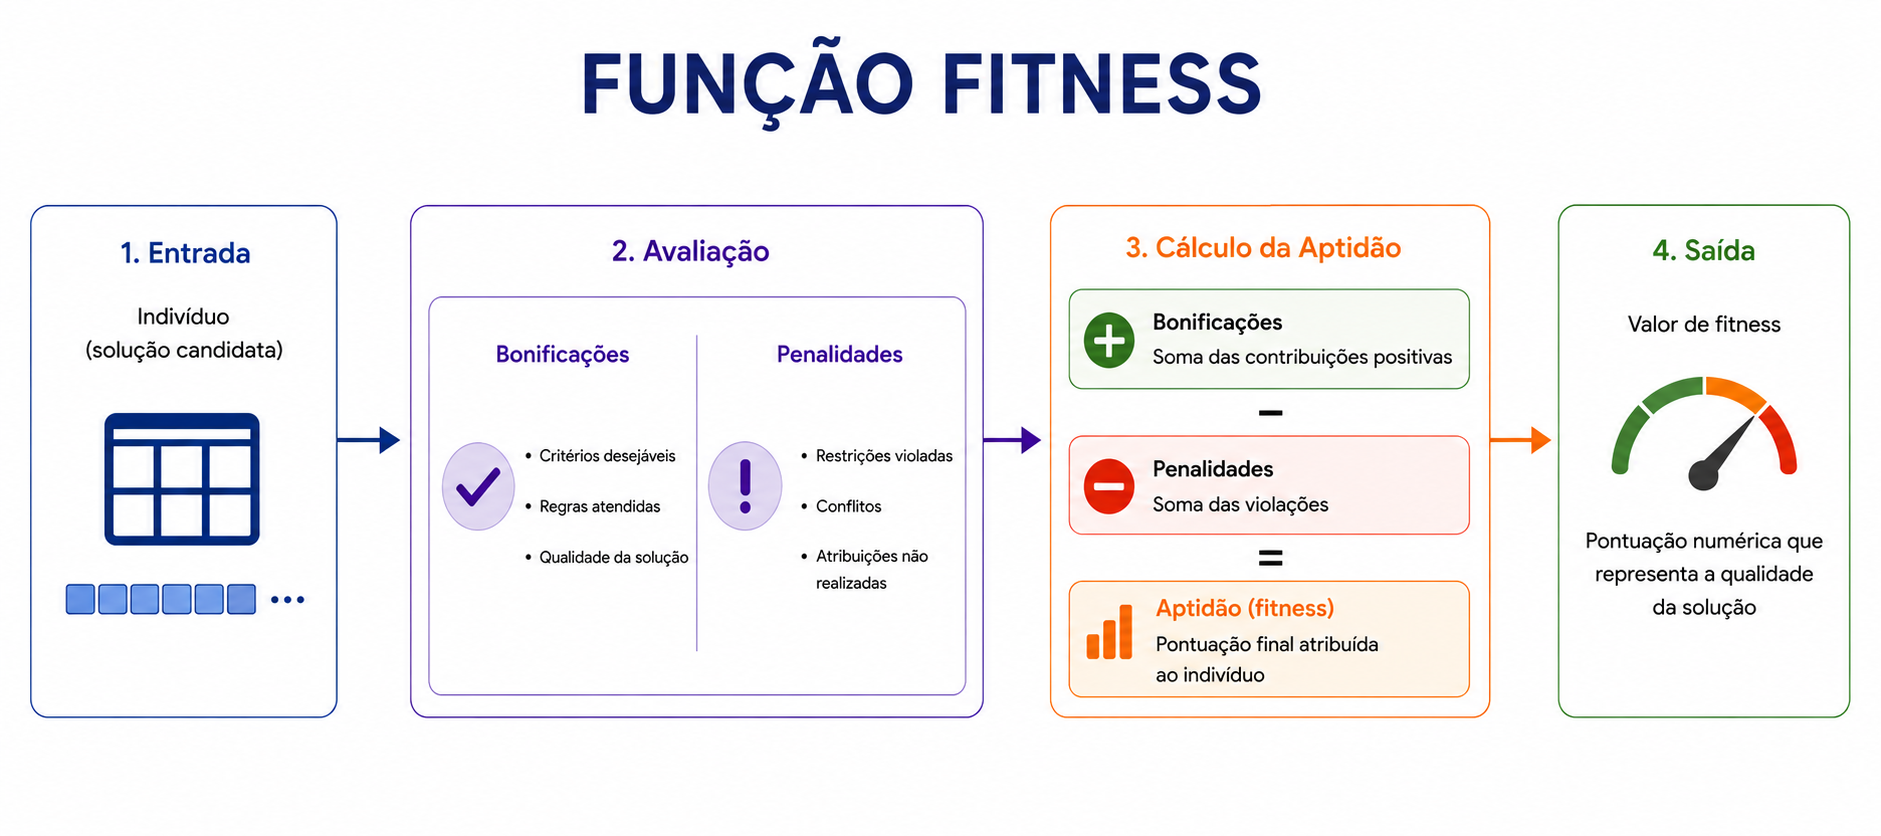
\includegraphics[width=0.85\textwidth]{figuras/Figura_1_ilustracaoFuncaoFitness.png}

\vspace{0.2cm}
\fonteautores
\end{figure}

\subsubsection{Seleção}
\label{subsubsec:selecao}

A seleção é o operador responsável por escolher quais indivíduos da população participarão do processo de reprodução e poderão contribuir para a formação da geração seguinte. Esse mecanismo representa, no contexto computacional, a pressão seletiva observada nos processos evolutivos naturais \cite{meniz2025}.

Em Algoritmos Genéticos, indivíduos com melhor valor de \textit{fitness} tendem a possuir maior probabilidade de serem selecionados. No entanto, a seleção não deve eliminar completamente indivíduos menos aptos, pois a manutenção de alguma diversidade populacional é importante para evitar a convergência prematura \cite{hussain2020}.

Entre os métodos de seleção mais utilizados estão a seleção por roleta, a seleção por torneio e a seleção por \textit{ranking}. A seleção por roleta atribui probabilidades proporcionais ao valor de \textit{fitness} de cada indivíduo. A seleção por torneio compara pequenos grupos de indivíduos e escolhe o mais apto entre eles. Já a seleção por \textit{ranking} considera a posição relativa dos indivíduos na população, reduzindo o impacto de diferenças absolutas muito grandes entre valores de aptidão \cite{meniz2025}.

\begin{figure}[H]
\centering
\caption{Seleção de indivíduos para reprodução em Algoritmos Genéticos}
\label{fig:selecao-individuos-ag}

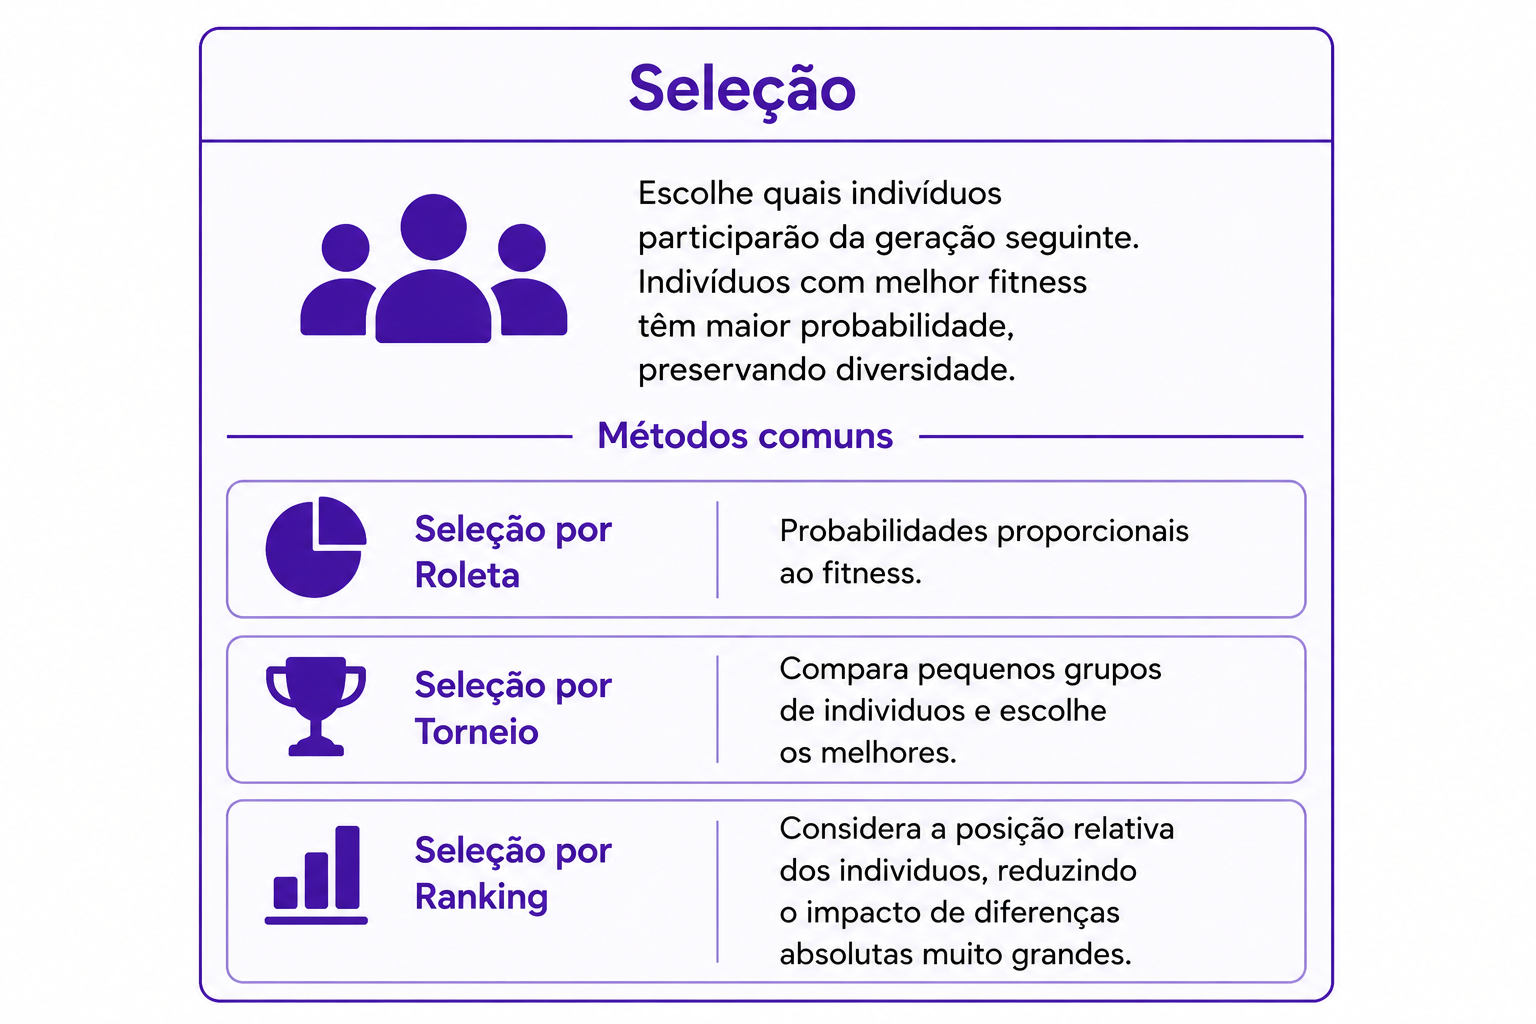
\includegraphics[width=0.85\textwidth]{figuras/Figura_2_ilustracaoAGSelecao.png}

\vspace{0.2cm}
\fonteautores
\end{figure}

\subsubsection{Crossover}
\label{subsubsec:crossover}

O \textit{crossover}, também chamado de cruzamento, corresponde ao operador de recombinação computacional. Sua função é combinar partes de dois ou mais indivíduos selecionados para gerar novos descendentes, preservando características de soluções consideradas promissoras \cite{umbarkar2015}.

Esse operador parte do princípio de que boas soluções podem conter componentes úteis que, quando recombinados com componentes de outras soluções, podem gerar indivíduos ainda mais adequados ao problema. Assim, o \textit{crossover} atua como mecanismo de exploração do espaço de busca, criando novas combinações a partir de informações já presentes na população \cite{fajrin2020}.

Existem diferentes estratégias de \textit{crossover}, como cruzamento de um ponto, cruzamento de múltiplos pontos e cruzamento uniforme. A escolha da estratégia depende da forma de codificação da solução e das restrições do problema. Em problemas de grades horárias, o operador deve ser projetado com cuidado, pois a troca inadequada de partes entre indivíduos pode gerar conflitos, como choques de professores, turmas ou horários \cite{umbarkar2015, fajrin2020}.

\begin{figure}[H]
\centering
\caption{Cruzamento de indivíduos em Algoritmos Genéticos}
\label{fig:crossover-ag}

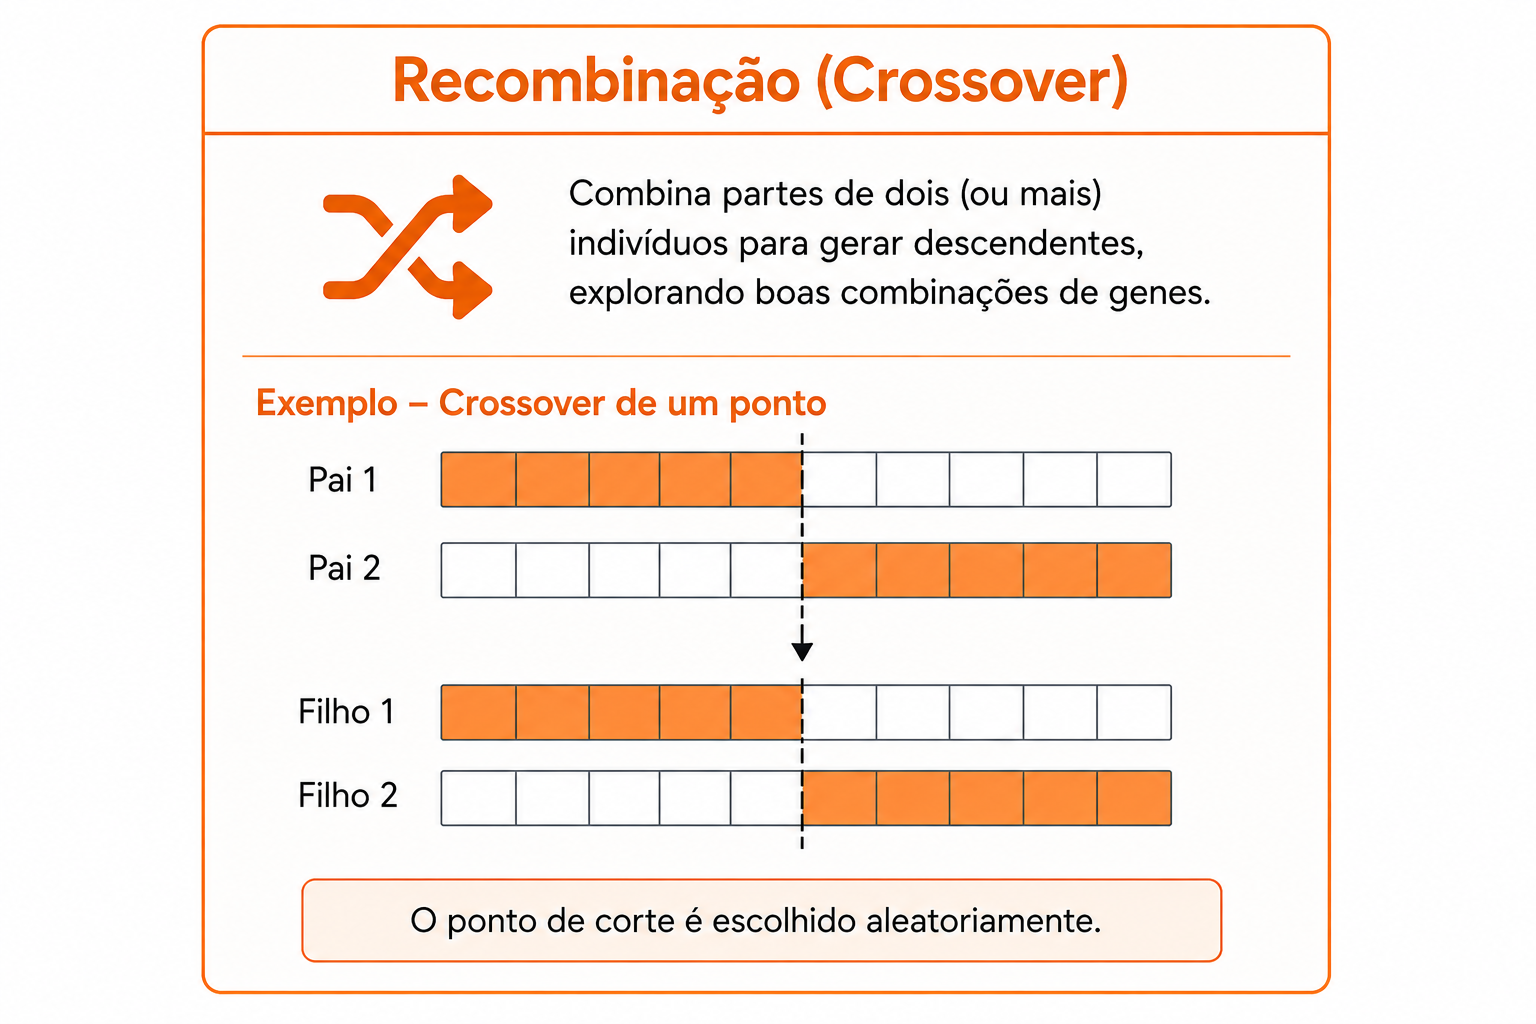
\includegraphics[width=0.85\textwidth]{figuras/Figura_3_ilustracaoAGCrossover.png}

\vspace{0.2cm}
\fonteautores
\end{figure}

\subsubsection{Mutação}
\label{subsubsec:mutacao}

A mutação é o operador responsável por introduzir alterações pontuais nos genes de um indivíduo. Seu papel é preservar a diversidade da população e permitir que o algoritmo explore regiões do espaço de busca que poderiam não ser alcançadas apenas por seleção e \textit{crossover} \cite{lengler2024}.

Em termos computacionais, a mutação pode modificar valores, trocar posições, substituir elementos ou alterar pequenas partes da solução, dependendo da representação adotada. Em um problema de timetabling universitário, por exemplo, uma mutação pode alterar o horário de uma aula, substituir uma alocação ou modificar a associação entre uma demanda acadêmica e determinado recurso disponível \cite{romaguera2024}.

Embora seja essencial para evitar a estagnação da busca, a mutação deve ser aplicada de forma controlada. Taxas muito baixas podem limitar a diversidade da população, enquanto taxas muito altas podem transformar o processo em uma busca excessivamente aleatória. Por isso, a taxa de mutação deve equilibrar exploração e estabilidade evolutiva \cite{cetin2020}.

Em problemas com muitas restrições, como o \textit{University Course Timetabling Problem} (UCTP), os operadores de seleção, \textit{crossover} e mutação exigem validação adicional, pois podem gerar soluções inválidas. Nesses casos, é comum empregar estratégias de penalização, reparo ou operadores especializados que preservem a viabilidade das soluções \cite{lagaros2023, romaguera2024}.

\begin{figure}[H]
\centering
\caption{Mutação em Algoritmos Genéticos}
\label{fig:mutacao-ag}

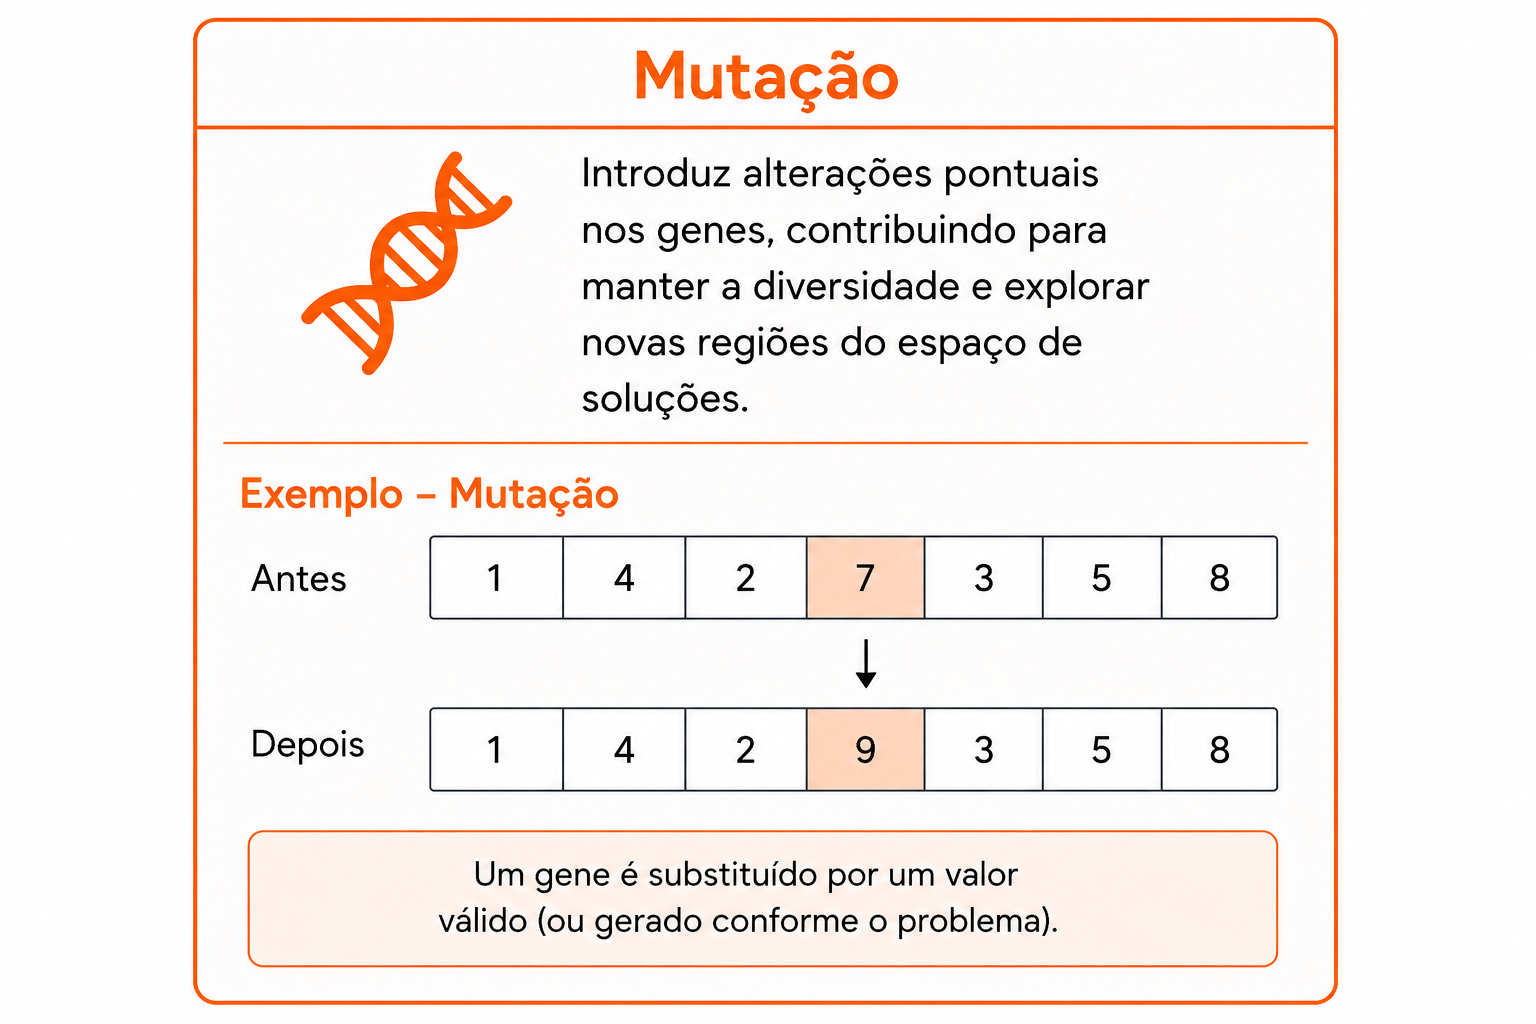
\includegraphics[width=0.85\textwidth]{figuras/Figura_4_ilustracaoAGMutacao.png}

\vspace{0.2cm}
\fonteautores
\end{figure}

\subsubsection{Tratamento de Restrições}
\label{subsubsec:tratamento-restricoes}

O tratamento de restrições é essencial em aplicações reais de Algoritmos Genéticos. Em problemas como o \textit{University Course Timetabling Problem} (UCTP), grande parte das combinações possíveis pode violar alguma regra, como conflito de professor, choque de turma ou incompatibilidade de horário \cite{abdipoor2023}.

As principais estratégias de tratamento incluem penalização, reparo, decodificação e operadores que preservam viabilidade. A penalização reduz o \textit{fitness} de soluções inválidas. O reparo tenta corrigir conflitos quando há alternativa possível. A decodificação transforma uma representação interna em uma solução válida. Já operadores restritivos buscam evitar a criação de indivíduos inviáveis desde o início \cite{rahimiConstraint2023, lagaros2023}.

A escolha da estratégia depende da natureza do problema e da forma como as restrições são modeladas. Em problemas altamente restritivos, a simples penalização pode não ser suficiente, pois a população pode permanecer concentrada em soluções inviáveis. Nesses casos, mecanismos de reparo ou operadores especializados tendem a contribuir para maior eficiência do processo evolutivo \cite{lagaros2023}.

\begin{figure}[H]
\centering
\caption{Tratamento de restrições em Algoritmos Genéticos}
\label{fig:tratamento-restricoes}

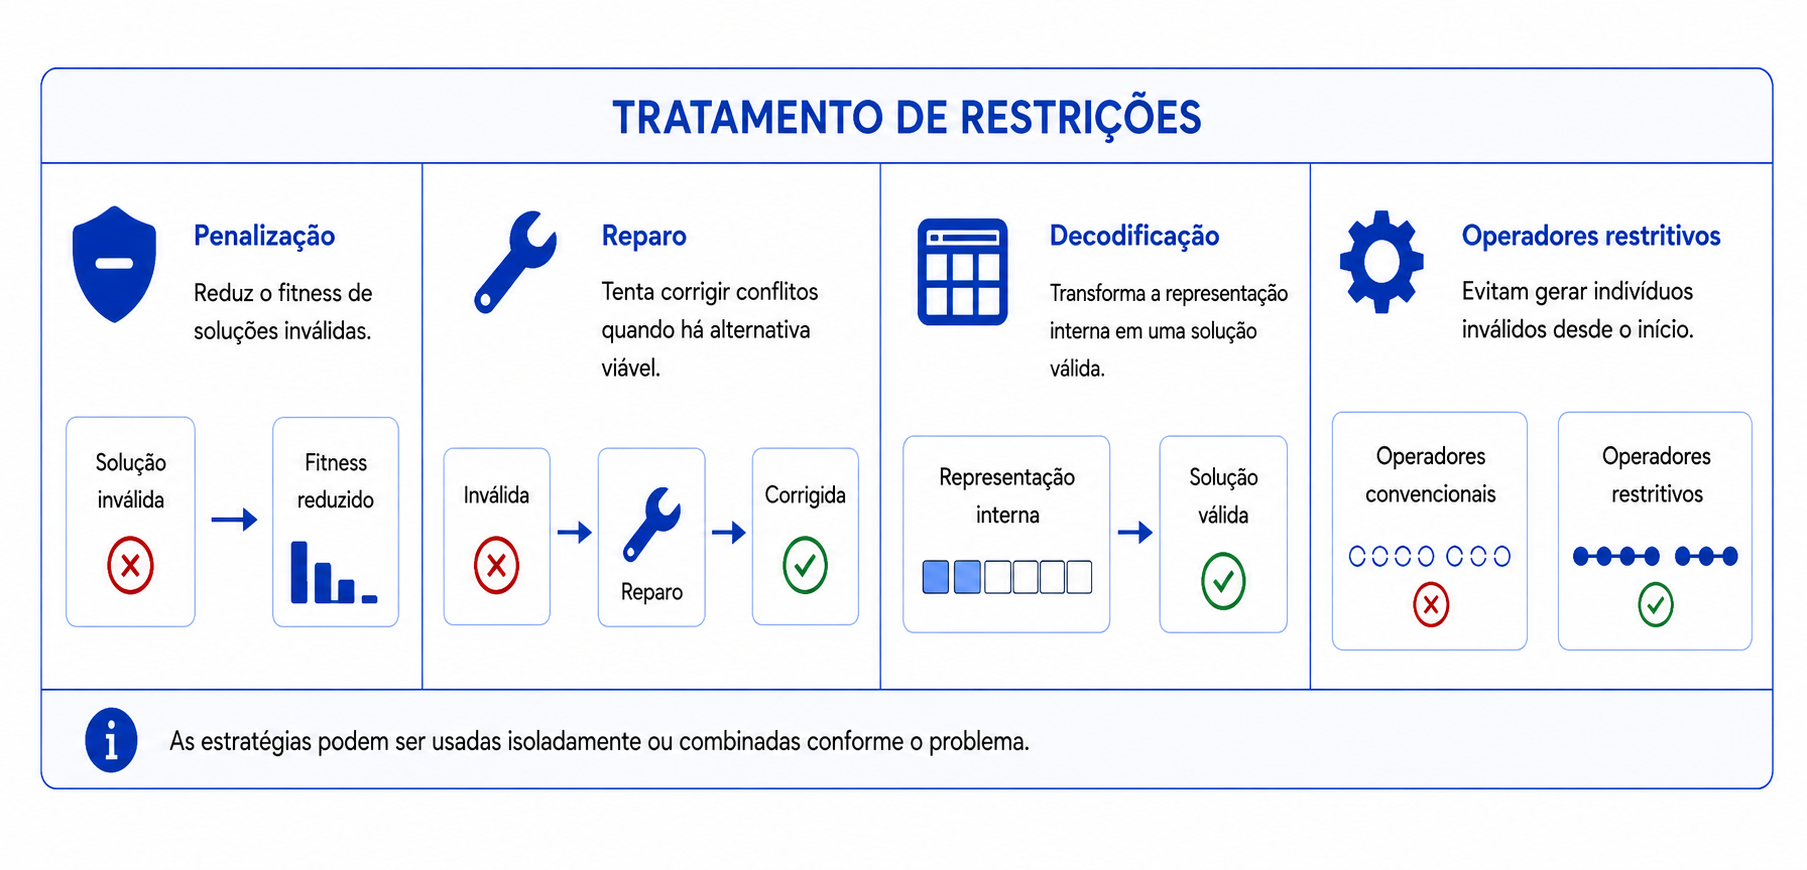
\includegraphics[width=0.85\textwidth]{figuras/Figura_5_ilustracaoAGTratamentoRestricoes.png}

\vspace{0.2cm}
\fonteautores
\end{figure}

\subsubsection{Convergência Prematura}
\label{subsubsec:convergencia-prematura}

Outro desafio importante em Algoritmos Genéticos é a convergência prematura. Esse fenômeno ocorre quando a população perde diversidade muito cedo e passa a se concentrar em uma região limitada do espaço de busca. Como consequência, o algoritmo pode estabilizar em uma solução localmente boa, mas distante de soluções potencialmente melhores \cite{cebeci2025}.

A convergência prematura está geralmente associada ao excesso de pressão seletiva, à baixa variabilidade introduzida pelos operadores genéticos ou ao uso inadequado de parâmetros. Fatores como tamanho da população, taxa de mutação, método de seleção e elitismo influenciam diretamente esse equilíbrio entre exploração e intensificação da busca \cite{cebeci2025, mustapha2026}.

Para reduzir esse problema, podem ser adotadas estratégias como aumento da diversidade populacional, ajuste da taxa de mutação, uso moderado de elitismo e escolha de métodos de seleção menos agressivos. Assim, busca-se preservar a capacidade de exploração do algoritmo ao longo das gerações, sem comprometer a evolução das soluções promissoras \cite{lengler2024, pytel2024}.

\begin{figure}[H]
\centering
\caption{Convergência Prematura em Algoritmos Genéticos}
\label{fig:convergencia-prematura}

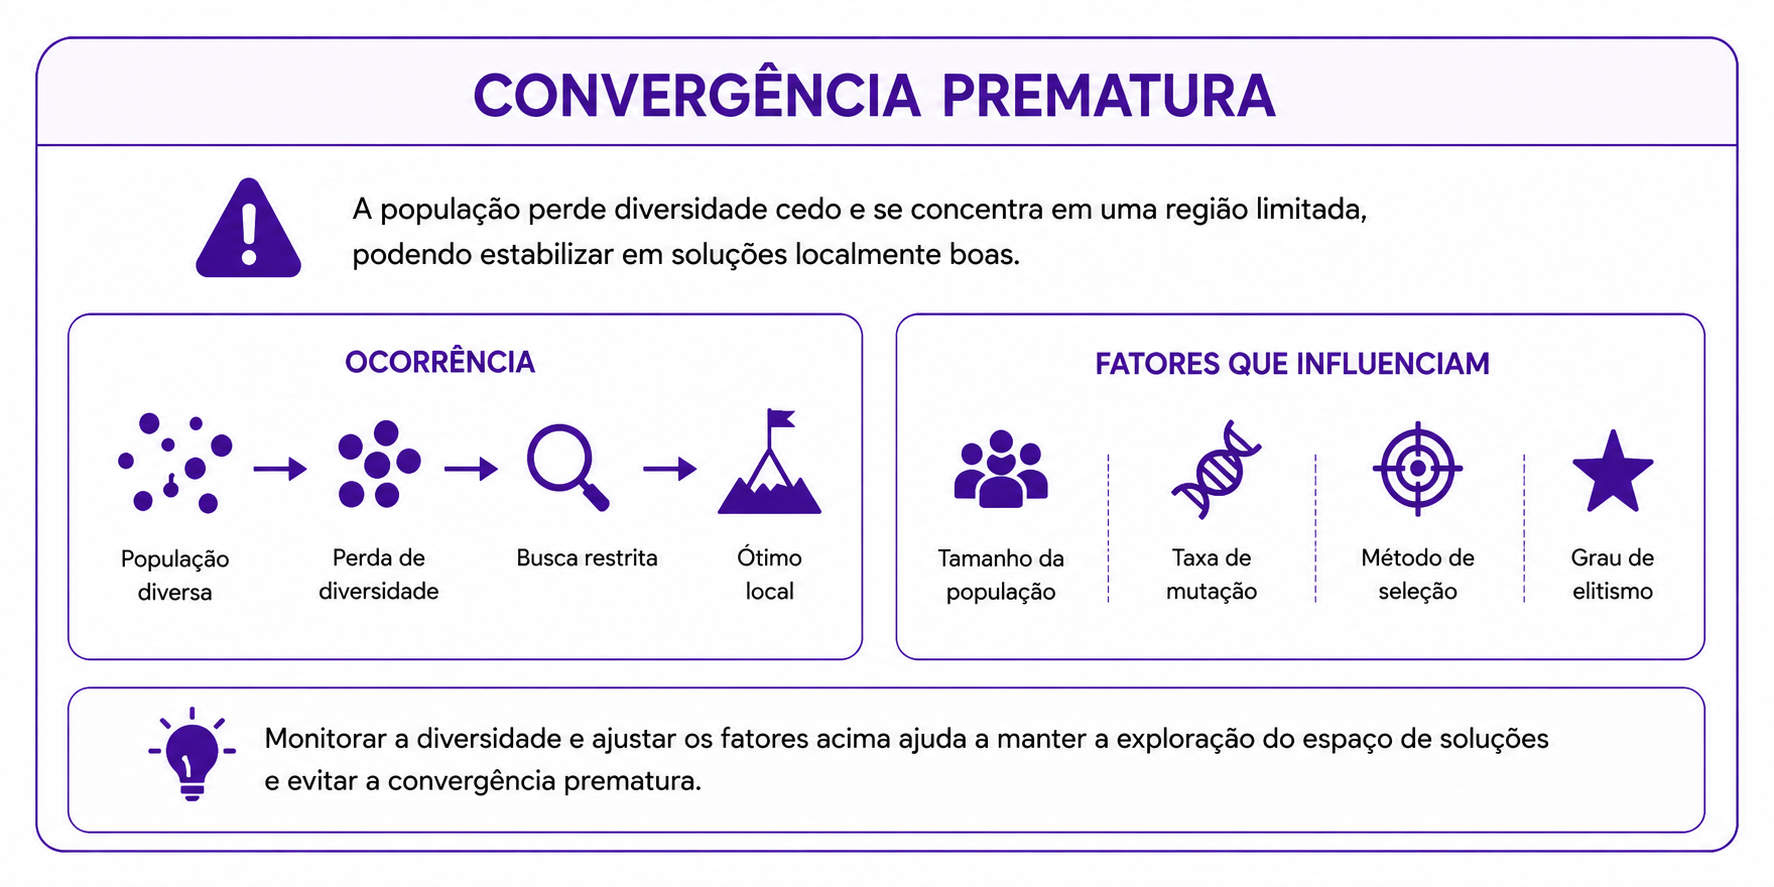
\includegraphics[width=0.85\textwidth]{figuras/Figura_6_ilustracaoAGConvergenciaPrematura.png}

\vspace{0.2cm}
\fonteautores
\end{figure}

\subsubsection{Ciclo de Execução e Pseudocódigo}
\label{subsubsec:ciclo-execucao-pseudocodigo}

O funcionamento geral de um Algoritmo Genético pode ser descrito como um ciclo evolutivo. Inicialmente, cria-se uma população de soluções candidatas. Em seguida, cada indivíduo é avaliado por uma função \textit{fitness}. Depois, o algoritmo seleciona indivíduos para reprodução, aplica \textit{crossover}, introduz mutações, avalia os novos indivíduos e forma uma nova população.

Esse processo é repetido até que o critério de parada seja satisfeito. Ao final, retorna-se a melhor solução encontrada segundo a função de avaliação adotada.

\begin{algorithm}[H]
\caption{Algoritmo Genético (BasicAG)}
\begin{enumerate}
\item População $\leftarrow$ InicializarPopulação()
\item AvaliarFitness(População)
\item repetir
\item Pais $\leftarrow$ SelecionarPais(População)
\item Filhos $\leftarrow$ Cruzamento(Pais)
\item Filhos $\leftarrow$ Mutação(Filhos)
\item AvaliarFitness(Filhos)
\item População $\leftarrow$ Substituir(População, Filhos)
\item até CritérioDeParadaSatisfeito()
\item retornar MelhorSolução(População)
\end{enumerate}
\end{algorithm}


\begin{figure}[H]
\centering
\caption{Representação gráfica do ciclo de execução de um Algoritmo Genético}
\label{fig:ilustracao-ag}

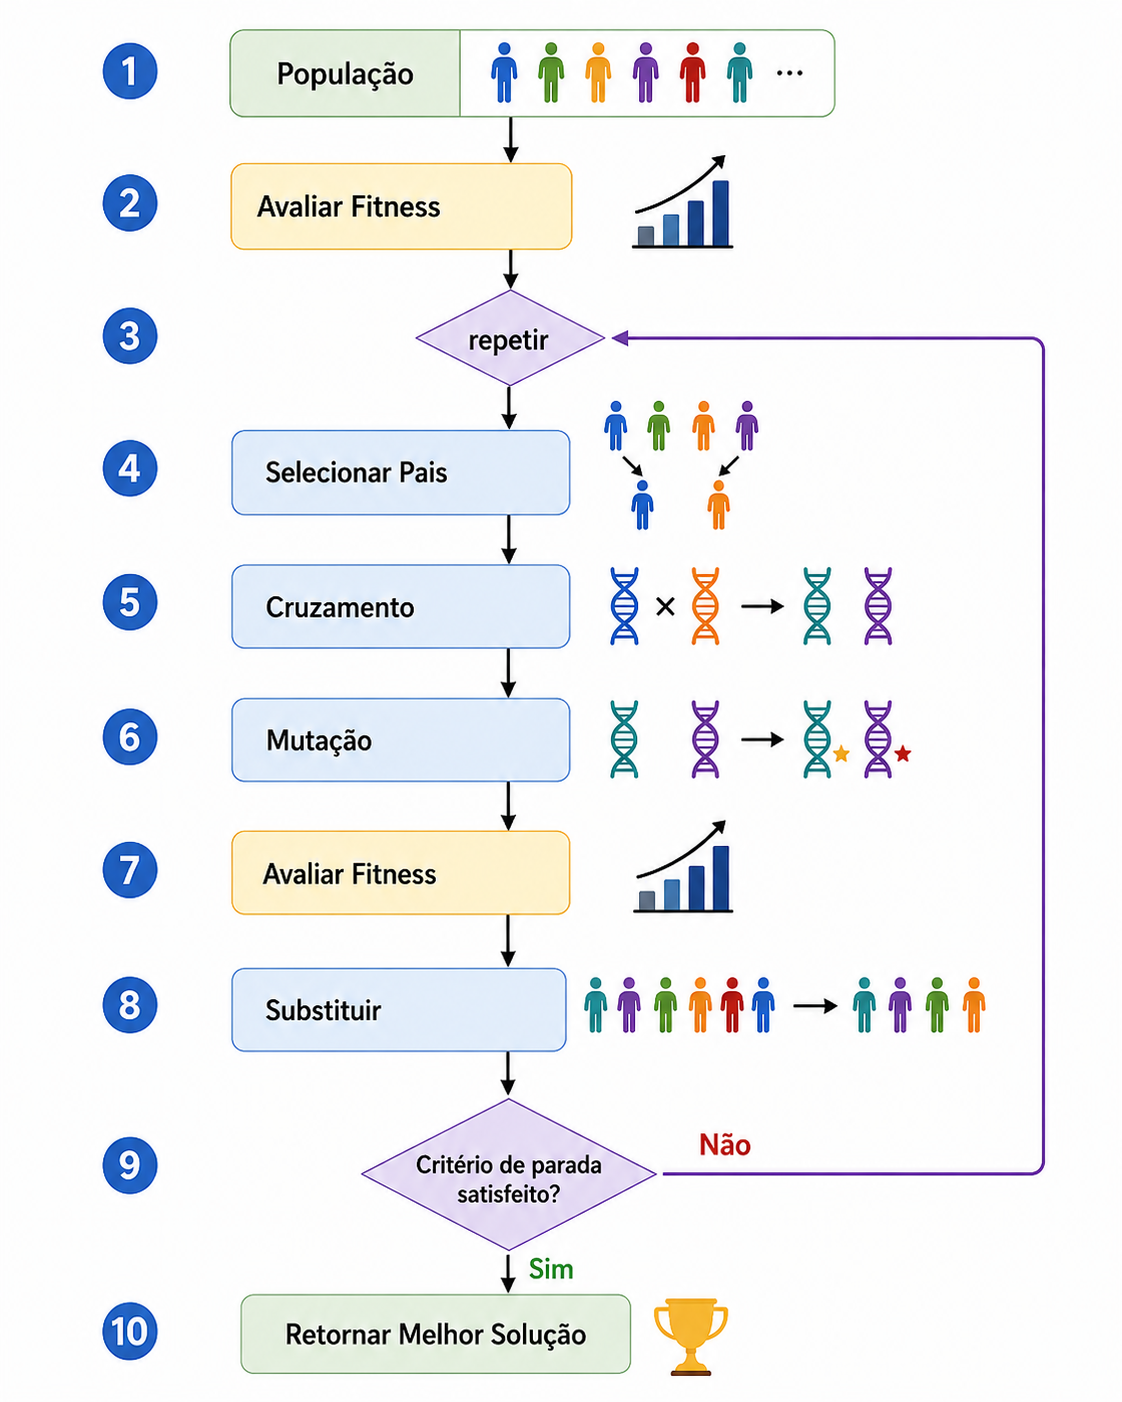
\includegraphics[width=0.85\textwidth]{figuras/Figura_7_ilustracaoAG.png}

\vspace{0.2cm}
\fonteautores
\end{figure}


Esse fluxo representa a estrutura geral dos Algoritmos Genéticos. Sua eficácia depende da adequação entre representação, função \textit{fitness}, operadores genéticos, tratamento de restrições e critérios de parada. No contexto do IGRIS, essa lógica fundamenta a geração automatizada de grades horárias acadêmicas, posteriormente detalhada nos capítulos de implementação.

\section{Arquitetura do Sistema e Integração entre Serviços}
\label{sec:2.4}

O desenvolvimento de sistemas de software complexos demanda escolhas arquiteturais capazes de equilibrar organização interna do código, desempenho operacional, manutenibilidade e capacidade de evolução. No caso do IGRIS, essa estrutura é formada pela combinação entre um monolito modular, responsável por concentrar os principais módulos da aplicação, e adaptadores de microsserviços, utilizados para integrar as diferentes implementações dos algoritmos genéticos.

O monolito modular é uma variação do monolito tradicional na qual a aplicação é executada como um único processo, mas organizada internamente em módulos separados e coesos. Cada módulo possui responsabilidades próprias e pode ser desenvolvido de forma relativamente independente, embora todos sejam combinados em um único artefato para implantação \cite[p.~15--16]{newman2021}. Diferentemente do monolito clássico, em que o crescimento do código tende a formar uma estrutura homogênea e fortemente acoplada, o monolito modular estabelece fronteiras explícitas entre responsabilidades de negócio dentro do mesmo processo. Essa organização preserva a clareza estrutural e reduz a complexidade operacional associada a arquiteturas distribuídas completas.

A arquitetura em camadas, conhecida como \textit{Layered Architecture}, organiza o fluxo de dados dentro dos módulos do sistema. Nessa abordagem, as responsabilidades são distribuídas entre camadas com papéis definidos: a camada de \textit{Controller} recebe e direciona as requisições HTTP; a camada de \textit{Service} concentra a lógica de negócio; a camada de \textit{Repository} abstrai o acesso ao banco de dados; e a camada de \textit{Model} representa as entidades do domínio \cite[Seção~6.3.1]{sommerville2016}. Essa separação reduz o acoplamento entre responsabilidades distintas, facilita a manutenção do código e favorece a realização de testes unitários.

\subsection{Adaptadores de Microsserviços e Comunicação REST}
\label{subsec:2.4.1}

Quando parte do processamento apresenta custo computacional elevado, como ocorre na geração de grades por Algoritmos Genéticos, sua execução pode comprometer a responsividade do sistema principal. Nesse cenário, o uso de serviços externos permite isolar esse processamento em componentes independentes, com ciclo de vida, linguagem e ambiente de execução próprios \cite[p.~3]{newman2021}. No IGRIS, essa integração ocorre por meio de adaptadores, componentes responsáveis por encapsular os detalhes de comunicação HTTP e traduzir as interfaces dos serviços externos para o vocabulário interno da aplicação.

A comunicação entre o sistema principal e os serviços externos ocorre via HTTP, seguindo princípios associados ao estilo REST, ou \textit{Representational State Transfer}. Nesse modelo, as requisições devem conter as informações necessárias para seu processamento, reduzindo a dependência de estado armazenado no servidor. Além disso, os recursos e operações são acessados por meio dos métodos semânticos do protocolo HTTP, como GET, POST, PUT e DELETE \cite[p.~3]{newman2021}. No contexto do IGRIS, o sistema principal envia aos serviços algorítmicos um \textit{payload} estruturado em JSON contendo os dados necessários para a geração da grade, e recebe como resposta os resultados processados em formato igualmente estruturado.

A containerização por meio do Docker permite que serviços implementados em linguagens distintas operem em ambientes isolados e reprodutíveis, comunicando-se pela rede interna da aplicação. Essa estratégia é especialmente relevante para o IGRIS, pois possibilita executar implementações desenvolvidas em Java, Python e Go sem exigir que todas compartilhem o mesmo ambiente de dependências. Além disso, a utilização de containers contribui para padronizar as condições de execução nos experimentos de benchmark, reduzindo interferências externas e tornando mais consistente a comparação entre as diferentes implementações do algoritmo genético \cite[p.~20]{newman2021}.

% Chapter 2
\section{Trabalhos Relacionados}
\label{sec:trabalhos_correlatos}

O desenvolvimento de soluções automatizadas para o agendamento de aulas e exames tem sido impulsionado pela aplicação de heurísticas e meta-heurísticas. Diversos estudos indicam que essas abordagens são adequadas para lidar com o amplo espaço de busca característico dos problemas de timetabling, especialmente em cenários nos quais a enumeração exaustiva se torna inviável.

Bashab et al. (2023) apresentam uma revisão abrangente sobre técnicas de otimização aplicadas à calendarização universitária, contemplando conceitos, metodologias, restrições, benchmarks e questões em aberto. O trabalho destaca que o university timetabling é tratado na literatura como um problema de otimização combinatória e de natureza não polinomial, no qual diferentes estratégias computacionais têm sido empregadas para buscar soluções de boa qualidade. Entre essas estratégias, os autores observam o uso recorrente de meta-heurísticas, métodos multiobjetivo e abordagens híbridas, especialmente pela capacidade dessas técnicas de tratar múltiplas restrições e critérios de avaliação em instâncias complexas.

\citeonline{awad2022} propuseram uma abordagem baseada em Busca Tabu Adaptativa para problemas de course timetabling em larga escala. A principal contribuição do estudo está no ajuste dinâmico da lista tabu, utilizado para melhorar o processo de busca e evitar estagnação em regiões pouco promissoras do espaço de soluções. A validação foi realizada com onze instâncias de benchmark originalmente apresentadas por Socha et al., compostas por problemas pequenos, médios e grandes. Os resultados indicaram que a abordagem foi capaz de produzir grades competitivas em comparação com métodos anteriores, reforçando a relevância da adaptação de parâmetros em meta-heurísticas aplicadas à calendarização acadêmica.

\citeonline{elen2022}, por sua vez, demonstrou a aplicação prática de Algoritmos Genéticos no problema de agendamento de exames. O estudo desenvolveu um método baseado em AG para o Vocational School of T.O.B.B. Technical Sciences, da Karabuk University, utilizando dados reais do período letivo de 2018-2019. A solução foi testada com 421 disciplinas, 54 docentes, 27 programas acadêmicos e 21 salas, obtendo horários de exame sem sobreposição em tempo médio de aproximadamente quatro minutos e em menos de 2000 iterações. Esse resultado evidencia a viabilidade do uso de Algoritmos Genéticos em sistemas de apoio à decisão voltados ao planejamento acadêmico.

Em conjunto, esses trabalhos demonstram que meta-heurísticas como Algoritmos Genéticos, Busca Tabu e abordagens híbridas constituem alternativas relevantes para problemas de calendarização acadêmica. Entretanto, observa-se que muitos estudos concentram-se na avaliação algorítmica isolada, sem necessariamente integrar a solução a um sistema operacional completo ou comparar diferentes paradigmas de implementação sob uma mesma arquitetura. Nesse ponto, o IGRIS se diferencia ao combinar a geração automatizada de grades com módulos de gestão acadêmica, interface de operação e benchmark controlado entre implementações desenvolvidas em Java, Python e Go.


\chapter{Metodologia}
\label{cap:metodologia}

\section{Metodologia da Pesquisa}
\label{sec:3.1}

Quanto à sua natureza, este trabalho classifica-se como pesquisa aplicada, pois tem como finalidade produzir conhecimento voltado à solução de um problema prático e delimitado: a automação da alocação de grades horárias em Instituições de Ensino Superior. Segundo \citeonline{gil2002}, a pesquisa aplicada caracteriza-se por estar orientada à aplicação prática dos conhecimentos produzidos, buscando responder a problemas concretos de determinado contexto. Nesse sentido, o presente estudo não se restringe à discussão teórica sobre o problema de timetabling universitário ou sobre Algoritmos Genéticos, mas propõe, implementa e avalia soluções computacionais integradas ao sistema IGRIS.

O problema investigado envolve a construção automatizada de grades horárias acadêmicas a partir de um conjunto de entidades e restrições, como turmas, disciplinas, professores, disponibilidades, turnos, matrizes curriculares e vínculos entre docentes e componentes curriculares. Trata-se de um problema de natureza combinatória, no qual o número de possibilidades cresce rapidamente conforme aumenta a quantidade de elementos envolvidos. Por esse motivo, a aplicação de técnicas heurísticas e meta-heurísticas torna-se relevante, uma vez que essas abordagens buscam encontrar soluções adequadas em tempo computacional viável, ainda que não garantam necessariamente a solução ótima global.

Do ponto de vista dos objetivos, a pesquisa classifica-se como exploratória e descritiva. A dimensão exploratória está associada à investigação da viabilidade técnica de diferentes implementações de Algoritmos Genéticos aplicadas ao mesmo problema. Conforme \citeonline{gil2002}, pesquisas exploratórias têm como finalidade proporcionar maior familiaridade com o problema, tornando-o mais explícito e permitindo o aprimoramento de ideias. Neste trabalho, essa característica manifesta-se na análise de três abordagens distintas, denominadas Sunny, Morpheus e Rocket, desenvolvidas com decisões próprias de implementação, integração e execução.

Complementarmente, a pesquisa possui caráter descritivo, pois registra, organiza e analisa sistematicamente o comportamento das implementações desenvolvidas. De acordo com \citeonline{prodanov2013}, a pesquisa descritiva busca observar, registrar e analisar fenômenos sem manipulá-los de forma arbitrária. No contexto deste trabalho, essa classificação se justifica pela coleta estruturada de métricas de benchmark, como tempo de execução, consumo de recursos computacionais e qualidade das soluções geradas. Assim, a pesquisa não apenas apresenta os algoritmos implementados, mas descreve seu comportamento em um cenário experimental controlado.

Quanto à abordagem do problema, o estudo possui natureza quantitativa e qualitativa, com predominância quantitativa na etapa de avaliação experimental. A dimensão quantitativa está presente na coleta e comparação de métricas numéricas obtidas durante os benchmarks. Esses dados permitem avaliar o desempenho das implementações sob critérios mensuráveis, reduzindo a subjetividade da análise comparativa. Conforme \citeonline{prodanov2013}, a pesquisa quantitativa considera que os fenômenos podem ser traduzidos em números, opiniões e informações classificáveis e analisáveis.

Entretanto, o trabalho também apresenta uma dimensão qualitativa, especialmente nas etapas de análise arquitetural, modelagem do domínio acadêmico e escolha dos dilemas de implementação. A comparação entre Sunny, Morpheus e Rocket não se limita aos valores numéricos obtidos nos testes, pois também envolve a interpretação das decisões de projeto, da estrutura de integração, da organização dos módulos e das características técnicas de cada solução. Dessa forma, embora a etapa de benchmark forneça a base quantitativa da avaliação, a análise qualitativa contribui para compreender as razões técnicas que podem influenciar os resultados observados.

Em relação aos procedimentos técnicos, esta pesquisa combina revisão bibliográfica estruturada e pesquisa experimental. A revisão bibliográfica foi utilizada para fundamentar os principais conceitos abordados no trabalho, incluindo o problema de timetabling universitário, Algoritmos Genéticos, heurísticas, meta-heurísticas, arquitetura de software, dilemas de programação e trabalhos relacionados. Segundo \citeonline{lakatos2003}, a pesquisa bibliográfica permite colocar o pesquisador em contato com o conhecimento já produzido sobre determinado tema, oferecendo base teórica para a construção da investigação.

A etapa bibliográfica foi conduzida a partir da análise de livros, artigos científicos, publicações técnicas e estudos correlatos. Essa fundamentação permitiu delimitar o problema, identificar abordagens já utilizadas na literatura e justificar a escolha dos Algoritmos Genéticos como estratégia de otimização. Também contribuiu para embasar as decisões relacionadas à arquitetura do sistema, à separação dos componentes e à comparação entre diferentes formas de implementação.

A pesquisa experimental, por sua vez, materializa-se na implementação e avaliação das três soluções propostas. Conforme \citeonline{gil2002}, a pesquisa experimental envolve a determinação de um objeto de estudo, a seleção das variáveis que podem influenciá-lo e a definição de formas de controle e observação dos efeitos produzidos. Neste trabalho, o objeto de estudo corresponde ao desempenho das implementações Sunny, Morpheus e Rocket na geração automatizada de grades horárias. As variáveis observadas incluem métricas de desempenho computacional e qualidade da solução, enquanto as condições de execução foram padronizadas para permitir comparação entre os algoritmos.

Para reduzir interferências externas, os benchmarks foram conduzidos sob condições equivalentes de hardware, base de entrada e parâmetros de execução. Essa padronização buscou garantir que as diferenças observadas entre Sunny, Morpheus e Rocket estivessem associadas principalmente às características das implementações, e não a variações acidentais do ambiente de teste. Foram executadas múltiplas requisições para cada algoritmo, totalizando 9.000 requisições por implementação, conforme o planejamento experimental apresentado no Capítulo 7.

O desenvolvimento do sistema seguiu uma estratégia iterativa e incremental, inspirada em práticas do Kanban. Essa abordagem foi adotada para organizar a construção gradual dos componentes do IGRIS e das implementações dos algoritmos. Conforme \citeonline{anderson2010}, o Kanban propõe tornar o fluxo de trabalho visível, limitar o trabalho em progresso e promover melhorias evolutivas no processo. No contexto deste trabalho, essas práticas foram operacionalizadas por meio da divisão das atividades em etapas de acompanhamento, como tarefas planejadas, tarefas em desenvolvimento, tarefas em validação e tarefas concluídas. Também foi considerada a limitação explícita de trabalho em progresso, conhecida como WIP Limit, a fim de evitar a execução paralela excessiva de tarefas e favorecer a finalização incremental dos módulos. Com base nessa organização, o desenvolvimento ocorreu em ciclos sucessivos de planejamento, implementação, validação e ajuste, permitindo que os componentes fossem construídos e avaliados progressivamente antes da integração final.

\section{Metodologia de Desenvolvimento}
\label{sec:3.2}

O desenvolvimento do IGRIS adotou o processo iterativo e incremental, no qual o produto é construído em ciclos sucessivos de planejamento, implementação e validação. Segundo \citeonline[p.~47]{sommerville2016}, essa abordagem é superior ao modelo cascata para projetos que envolvem requisitos em evolução ou componentes de alta complexidade técnica, como algoritmos de otimização, pois permite a validação contínua de cada incremento antes de avançar para o seguinte.

Cada ciclo de desenvolvimento foi organizado segundo o Official Kanban Guide \cite{kanbanuniversity2020}, que estrutura o fluxo de trabalho em colunas visuais representando estados de execução (a fazer, em progresso, concluído), com limitação explícita do trabalho em progresso (\textit{Work-in-Progress Limit}). Esse método reduz o acúmulo de tarefas simultâneas e aumenta a previsibilidade das entregas, favorecendo o controle do andamento em um projeto com múltiplos componentes interdependentes backend, microsserviços e frontend.

A integração entre os componentes foi validada de forma incremental: o Backend Core (Igris) foi desenvolvido e estabilizado primeiro, estabelecendo o contrato de API; em seguida, os microsserviços Sunny e Morpheus foram integrados sequencialmente ao ecossistema Docker; por fim, o Rocket foi incorporado como terceira implementação do algoritmo genético para fins de benchmark comparativo.

\section{Engenharia de Requisitos}
\label{sec:3.3}

A Engenharia de Requisitos é a disciplina que identifica, documenta e gerencia as necessidades dos stakeholders, estabelecendo o contrato funcional e de qualidade entre o sistema a ser desenvolvido e seus usuários \cite[p.~83]{sommerville2016}. No contexto do IGRIS, os requisitos foram levantados a partir das necessidades operacionais de coordenadores acadêmicos, professores e administradores de IES, e organizados em duas categorias: Requisitos Funcionais que descrevem os comportamentos que o sistema deve prover e Requisitos Não Funcionais que estabelecem os critérios de qualidade, desempenho e restrições arquiteturais.

\subsection{Requisitos Funcionais}
\label{subsec:3.3.1}

Os requisitos funcionais descrevem os comportamentos específicos que o software deve fornecer aos usuários para cumprir seu propósito. Segundo \citeonline{sommerville2016}, esses requisitos definem o que o sistema deve fazer e descrevem como o sistema responde a entradas, interações ou eventos específicos. O Quadro~\ref{tab:rf} apresenta os requisitos funcionais do IGRIS, organizados por domínio funcional.

\tituloquadro{tab:rf}{Requisitos Funcionais do IGRIS}

\begin{longtable}{|C{1.8cm}|L{4.5cm}|L{7.1cm}|}
\hline
\textbf{Código} & \textbf{Requisito} & \textbf{Descrição} \\
\hline
\endfirsthead
\hline
\textbf{Código} & \textbf{Requisito} & \textbf{Descrição} \\
\hline
\endhead
RF01 & Manter Disciplinas & O sistema deve ser capaz de manter disciplinas. \\
\hline
RF02 & Manter Turmas & O sistema deve ser capaz de manter turmas. \\
\hline
RF03 & Manter Cursos & O sistema deve ser capaz de manter cursos. \\
\hline
RF04 & Vincular Disciplinas a Cursos & O sistema deve ser capaz de vincular e manter a relação de quais disciplinas pertencem a quais cursos. \\
\hline
RF05 & Manter Matrizes Curriculares & O sistema deve ser capaz de manter matrizes curriculares (associação que define quais disciplinas compõem uma turma no semestre). \\
\hline
RF06 & Manter Turnos Letivos & O sistema deve ser capaz de manter turnos letivos (ex.: Matutino, Noturno). \\
\hline
RF07 & Manter Dias da Semana Letivos & O sistema deve ser capaz de manter dias da semana letivos. \\
\hline
RF08 & Manter Disponibilidade Docente & O professor deve ser capaz de informar e manter sua disponibilidade de dias e horários para lecionar. \\
\hline
RF09 & Gerar Grade Automatizada & O sistema deve ser capaz de gerar a grade de horários de forma automatizada (integração com microsserviços). \\
\hline
\end{longtable}

\newpage
\begin{longtable}{|C{1.8cm}|L{4.5cm}|L{7.1cm}|}
\hline
\textbf{Código} & \textbf{Requisito} & \textbf{Descrição} \\
\hline
\endhead
RF10 & Salvar Grade Gerada & O sistema deve ser capaz de salvar a grade gerada. \\
\hline
RF11 & Visualizar Grade e Histórico & O coordenador/administrador deve ser capaz de visualizar a grade gerada no semestre e acessar o histórico de grades. \\
\hline
RF12 & Manter Instituições & O sistema deve ser capaz de manter instituições (Faculdades/Universidades). \\
\hline
RF13 & Manter Coordenações & O sistema deve ser capaz de manter coordenações. \\
\hline
RF14 & Manter Coordenadores & O sistema deve ser capaz de manter coordenadores, vinculados a instituições e coordenações. \\
\hline
RF15 & Gerenciar Professores & O coordenador deve ser capaz de gerenciar os professores vinculados à sua instituição. \\
\hline
RF16 & Associar Professores a Disciplinas & O sistema deve ser capaz de associar professores às disciplinas que lecionam. \\
\hline
RF17 & Manter Configurações por Instituição & O administrador deve ser capaz de manter configurações e vínculos específicos por instituição. \\
\hline
RF18 & Gerar Link de Cadastro & O coordenador deve ser capaz de gerar um link exclusivo para o cadastro facilitado de novos professores. \\
\hline
\end{longtable}

\newpage
\begin{longtable}{|C{1.8cm}|L{4.5cm}|L{7.1cm}|}
\hline
\textbf{Código} & \textbf{Requisito} & \textbf{Descrição} \\
\hline
\endhead
RF19 & Validar Usuários via Link & O coordenador deve ser capaz de validar usuários cadastrados via link, ativando ou desativando seus acessos. \\
\hline
RF20 & Vincular Coordenador a Curso & O sistema deve ser capaz de vincular coordenadores a cursos específicos dentro de uma instituição. \\
\hline
RF21 & Manter Cadastro de Usuários & O sistema deve ser capaz de manter o cadastro global de usuários. \\
\hline
RF22 & Manter Perfis de Acesso & O sistema deve ser capaz de manter os perfis de acesso dos usuários. \\
\hline
RF23 & Múltiplos Perfis por Usuário & O usuário deve ser capaz de ter múltiplos perfis associados à sua conta. \\
\hline
RF24 & Alterar Perfil Ativo & O usuário deve ser capaz de alterar o seu perfil ativo de visualização enquanto logado. \\
\hline
RF25 & Login Autenticado & O usuário deve ser capaz de realizar login autenticado no sistema. \\
\hline
RF26 & Recuperação de Senha & O usuário deve ser capaz de solicitar a recuperação de senha via link de e-mail. \\
\hline
RF27 & Troca de Senha & O usuário deve ser capaz de trocar sua própria senha de forma segura. \\
\hline
\end{longtable}

\newpage
\begin{longtable}{|C{1.8cm}|L{4.5cm}|L{7.1cm}|}
\hline
\textbf{Código} & \textbf{Requisito} & \textbf{Descrição} \\
\hline
\endhead
RF28 & Configurar Parâmetros do AG & O administrador deve ser capaz de alterar os parâmetros matemáticos dos microsserviços (tamanho de população, gerações, \textit{crossover}, mutação etc.). \\
\hline
RF29 & Configurações Globais em Runtime & O administrador deve ser capaz de alterar parâmetros globais do sistema em tempo de execução, sem reinicialização. \\
\hline
RF30 & Enviar Feedback & O usuário deve ser capaz de enviar feedbacks descritivos sobre o sistema. \\
\hline
RF31 & Manter Categorias de Feedback & O administrador deve ser capaz de manter as categorias de classificação de feedbacks. \\
\hline
RF32 & Visualizar Própria Grade & O professor deve ser capaz de visualizar sua grade horária ativa. \\
\hline
RF33 & Ciclo de Vida das Grades & O sistema deve gerenciar automaticamente o ciclo de vida das grades: inativar a anterior ao gerar nova; inativar ao encerrar o semestre. \\
\hline
RF34 & Bloqueio de Disponibilidade & Enquanto houver grade ativa, o professor não deve ser capaz de alterar sua disponibilidade; apenas o coordenador pode. \\
\hline
RF35 & Notificação por E-mail & O sistema deve enviar automaticamente e-mail notificando os professores quando uma grade for ativada ou inativada. \\
\hline
\end{longtable}

\fonteautores

\subsection{Requisitos Não Funcionais}
\label{subsec:3.3.2}

Enquanto os requisitos funcionais definem o que o sistema deve fazer, os requisitos não funcionais estabelecem os critérios de qualidade, desempenho e restrições que a solução deve respeitar \cite[p.~86]{sommerville2016}. O Quadro~\ref{tab:rnf} consolida os requisitos não funcionais do IGRIS.

\tituloquadro{tab:rnf}{Requisitos Não Funcionais do IGRIS}

\begin{longtable}{|C{1.8cm}|L{4.5cm}|L{7.1cm}|}
\hline
\textbf{Código} & \textbf{Requisito} & \textbf{Descrição} \\
\hline
\endfirsthead
\hline
\textbf{Código} & \textbf{Requisito} & \textbf{Descrição} \\
\hline
\endhead
RNF01 & Arquitetura em Camadas & O sistema principal deve seguir o padrão de Arquitetura em Camadas (Layered Architecture). \\
\hline
RNF02 & Escalabilidade via Microsserviços & O cálculo pesado da geração de grades deve ser desacoplado da API principal, processado por microsserviços dedicados. \\
\hline
RNF03 & API RESTful & A aplicação de backend deve seguir inteiramente os princípios RESTful. \\
\hline
RNF04 & Autenticação Stateless (JWT) & A comunicação cliente-servidor deve ser stateless, utilizando tokens JWT injetados via cookies ou cabeçalhos. \\
\hline
RNF05 & Criptografia de Senhas & As senhas nunca devem ser armazenadas em texto plano, utilizando hash com salt (ex.: BCrypt). \\
\hline
RNF06 & Controle de Acesso (RBAC) & O sistema deve implementar controle de acesso baseado em papéis (RBAC), verificando permissões por rota. \\
\hline
RNF07 & Geração de Grade Assíncrona & A geração da grade deve rodar de forma assíncrona, com o frontend exibindo indicador de progresso. \\
\hline
RNF08 & Cache em Memória & O sistema deve utilizar cache em memória (ex.: Caffeine) para mitigar consultas frequentes ao banco de dados. \\
\hline
RNF09 & Integridade Referencial & A aplicação deve manter rigorosamente a integridade referencial dos dados com chaves estrangeiras. \\
\hline
\end{longtable}

\newpage
\begin{longtable}{|C{1.8cm}|L{4.5cm}|L{7.1cm}|}
\hline
\textbf{Código} & \textbf{Requisito} & \textbf{Descrição} \\
\hline
\endhead
RNF10 & Exclusão Lógica & Registros críticos devem priorizar exclusão lógica (Soft Delete) em vez de exclusão física permanente. \\
\hline
RNF11 & Auditoria e Logging & O sistema deve manter logs estruturados de acessos, erros e operações cruciais. \\
\hline
RNF12 & Padrão de Resposta JSON & A API deve envelopar todas as respostas em padrão JSON unificado, nunca expondo stack trace nativo ao cliente. \\
\hline
RNF13 & Comunicação Inter-serviços & Os microsserviços devem se comunicar via HTTP/REST pela rede interna Docker, sem exposição direta ao exterior. \\
\hline
RNF14 & Configuração Dinâmica & Os parâmetros do algoritmo genético devem ser ajustáveis em tempo de execução, sem reinicialização dos servidores. \\
\hline
RNF15 & Containerização & Todos os componentes devem ser containerizados via Docker para garantir reprodutibilidade dos ambientes. \\
\hline
RNF16 & Notificação por E-mail & O sistema deve ser capaz de enviar e-mails transacionais para notificação de professores. \\
\hline
RNF17 & Testes de Integração & O sistema deve possuir testes de integração automatizados cobrindo os fluxos críticos de negócio. \\
\hline
RNF18 & Suporte Multi-instituição & O sistema deve suportar múltiplas instituições de ensino de forma isolada na mesma instância. \\
\hline
\end{longtable}

\fonteautores
\setcounter{table}{0}



\chapter{Modelagem do Sistema}
\label{cap:modelagem}

Este capítulo apresenta a modelagem e a arquitetura do sistema IGRIS, descrevendo as decisões de projeto que conectam os requisitos identificados à implementação técnica. A modelagem é organizada em quatro perspectivas complementares: a arquitetura do sistema e seus componentes; a modelagem funcional e comportamental, representada pelos atores e casos de uso; a modelagem estrutural, expressa pelo diagrama de classes; e a modelagem de dados, formalizada pelo Modelo Entidade-Relacionamento e pelo dicionário de dados.

\section{Arquitetura do Sistema}
\label{sec:4.1}

O IGRIS adota um Monolito Modular com Adaptadores de Microsserviços, combinando a organização interna por módulos de domínio com o desacoplamento externo de componentes computacionalmente intensivos. O núcleo da aplicação é um único processo Spring Boot organizado em módulos coesos acadêmico, usuário, instituição, grade, segurança e comum, que se comunicam internamente sem latência de rede. Para a execução do Algoritmo Genético, o sistema delega o processamento a microsserviços independentes via adaptadores HTTP, isolando a lógica pesada de otimização sem comprometer a responsividade da API principal \cite[p.~15--16]{newman2021}.

A comunicação entre o Backend Core e os microsserviços ocorre de forma síncrona: o backend monta um \textit{payload} JSON com disponibilidades, matrizes, turmas e parâmetros do algoritmo, envia por HTTP POST ao microsserviço selecionado e recebe uma resposta estruturada contendo a grade otimizada, métricas de execução e lista de conflitos. Os parâmetros do algoritmo são armazenados na tabela \texttt{config\_sistema} e carregados em cache, permitindo ajuste em tempo de execução sem reinicialização \cite[p.~3]{newman2021}.

A arquitetura é composta por quatro serviços principais:

\begin{itemize}
  \item \textbf{Igris (Backend Core):} API principal em Java 17 com Spring Boot 3.5. Gerencia todas as operações CRUD do domínio acadêmico, autenticação JWT, controle de acesso RBAC e orquestra as chamadas aos microsserviços de otimização. É o único componente com acesso direto ao banco de dados PostgreSQL 15.
  \item \textbf{Sunny:} Microsserviço de geração de grade em Java com Spring Boot, implementando o Algoritmo Genético no paradigma orientado a objetos.
  \item \textbf{Morpheus:} Microsserviço equivalente em Python com Flask, implementando o mesmo algoritmo no paradigma funcional, com parada antecipada e melhoria local explícita.
  \item \textbf{Rocket:} Microsserviço em Go, implementando o AG com modelo de concorrência baseado em \textit{goroutines} e \textit{channels} (CSP). Representa o paradigma concorrente no benchmark comparativo \cite{coxbuday2017}.
\end{itemize}

Todos os componentes são containerizados via Docker e se comunicam pela rede interna \texttt{igris-network}, sem exposição direta ao exterior. O frontend React acessa exclusivamente o Backend Core na porta 8080 \cite[p.~20]{newman2021}.

\begin{figure}[H]
\centering
\caption{Arquitetura do sistema IGRIS}
\label{fig:arquitetura}

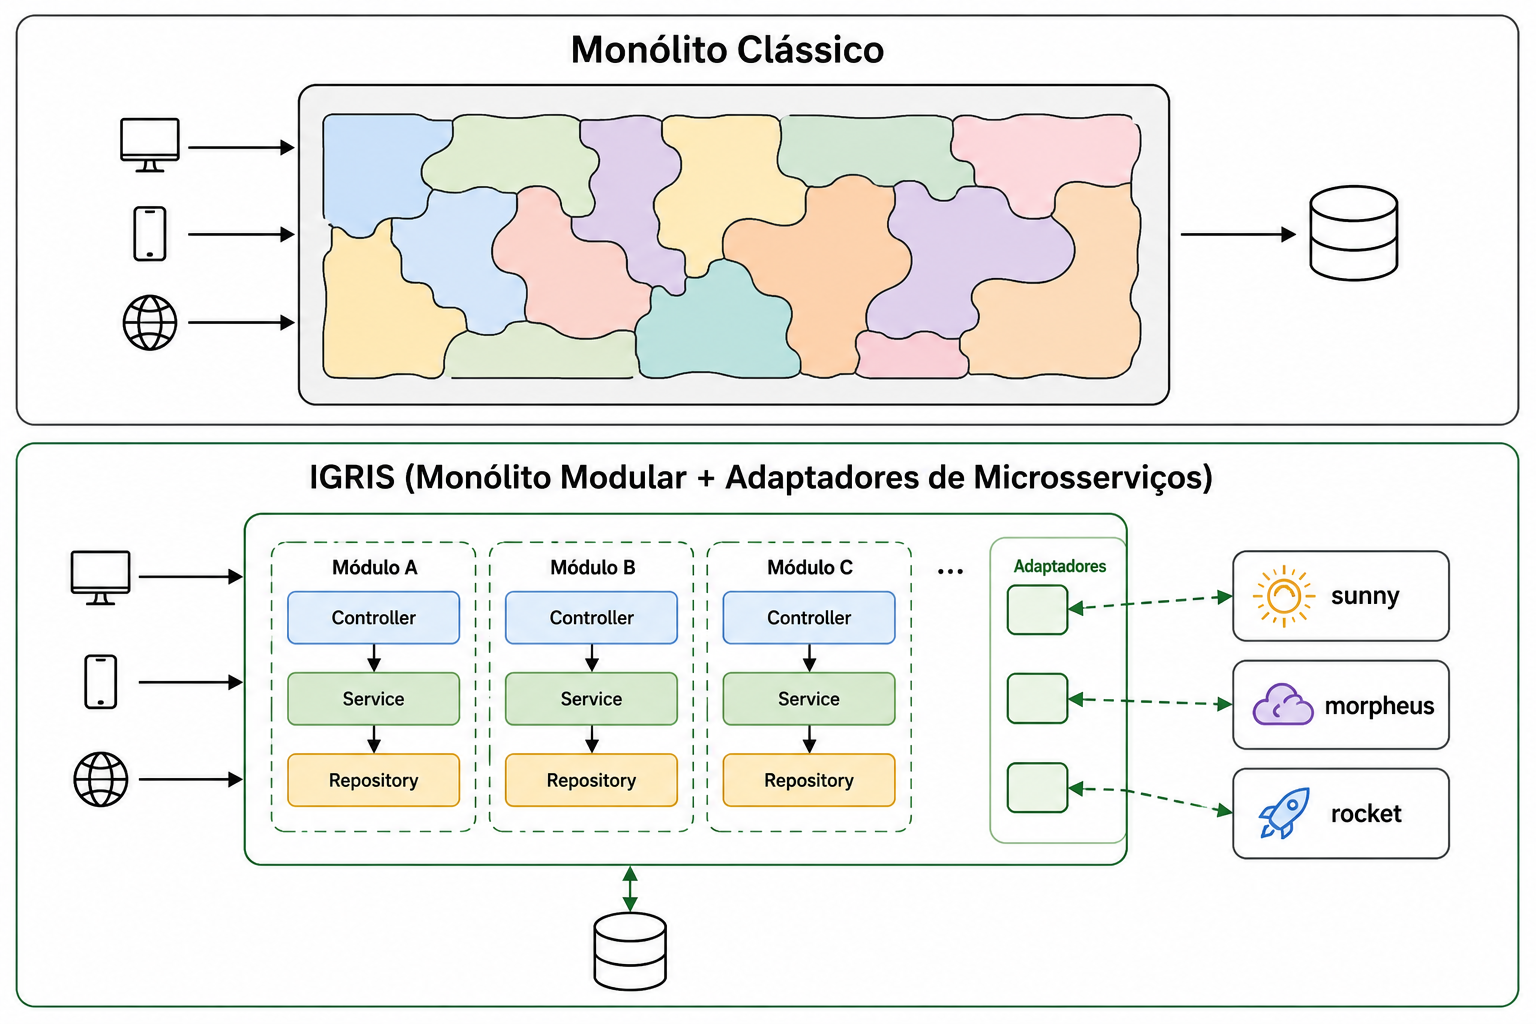
\includegraphics[width=0.85\textwidth]{figuras/Figura_8_ilustracaoArquitetura.png}

\vspace{0.2cm}
\fonteautores
\end{figure}
\section{Modelagem Funcional e Comportamental}
\label{sec:4.2}

A modelagem funcional tem como objetivo descrever as interações entre os usuários e o sistema, delimitando o escopo das funcionalidades e o comportamento esperado frente a diferentes cenários de uso. Segundo \citeonline{pressman2016}, essa etapa é fundamental para validar se os requisitos levantados correspondem às expectativas dos stakeholders, servindo como guia visual e textual para o desenvolvimento.

\subsection{Atores do Sistema}
\label{subsec:4.2.1}

O sistema IGRIS é composto por cinco atores, cada um com responsabilidades bem delimitadas conforme ilustrado no Diagrama de Casos de Uso.

O usuário representa o ator base do sistema. Todo acesso ao IGRIS é autenticado, cabendo ao usuário as operações comuns: autenticar-se, selecionar ou trocar de perfil, recuperar senha, realizar cadastro via link de convite e enviar feedback.

O coordenador é o ator gestor do fluxo acadêmico. Suas responsabilidades abrangem manter a disponibilidade dos professores, gerenciar disciplinas, turmas, cursos e matrizes, vincular disciplinas a cursos, manter turnos e dias letivos, gerar o link de cadastro de professores, além de gerar, salvar e visualizar a grade horária.

O professor alimenta o sistema com suas próprias informações: mantém sua disponibilidade de horários, registra as disciplinas que leciona e visualiza a própria grade gerada.

A instituição é responsável por operações de gestão de coordenadores: manter coordenadores e coordenações vinculadas à instituição.

O administrador do sistema possui acesso privilegiado: concede ou revoga perfis de acesso, mantém configurações globais do sistema, gerencia instituições e usuários, visualiza feedbacks e mantém as configurações de geração de grade, incluindo os parâmetros matemáticos dos microsserviços.

\subsection{Diagrama de Casos de Uso}
\label{subsec:4.2.2}

O Diagrama de Casos de Uso do IGRIS representa graficamente todas as interações possíveis entre os cinco atores do sistema e suas respectivas funcionalidades, organizadas por perfil de acesso e nível de responsabilidade. O diagrama consolida em uma única visão as operações de cada ator: desde as funcionalidades comuns ao Usuário (autenticação, seleção de perfil, feedback), passando pelas responsabilidades do Coordenador (gestão acadêmica completa e geração de grade), do Professor (disponibilidade e disciplinas lecionadas), da Instituição (gestão de coordenação) e do Administrador do Sistema (configuração e controle de acesso).

\begin{figure}[p]
\centering
\caption{Diagrama de Casos de Uso do IGRIS}
\label{fig:casos_de_uso}
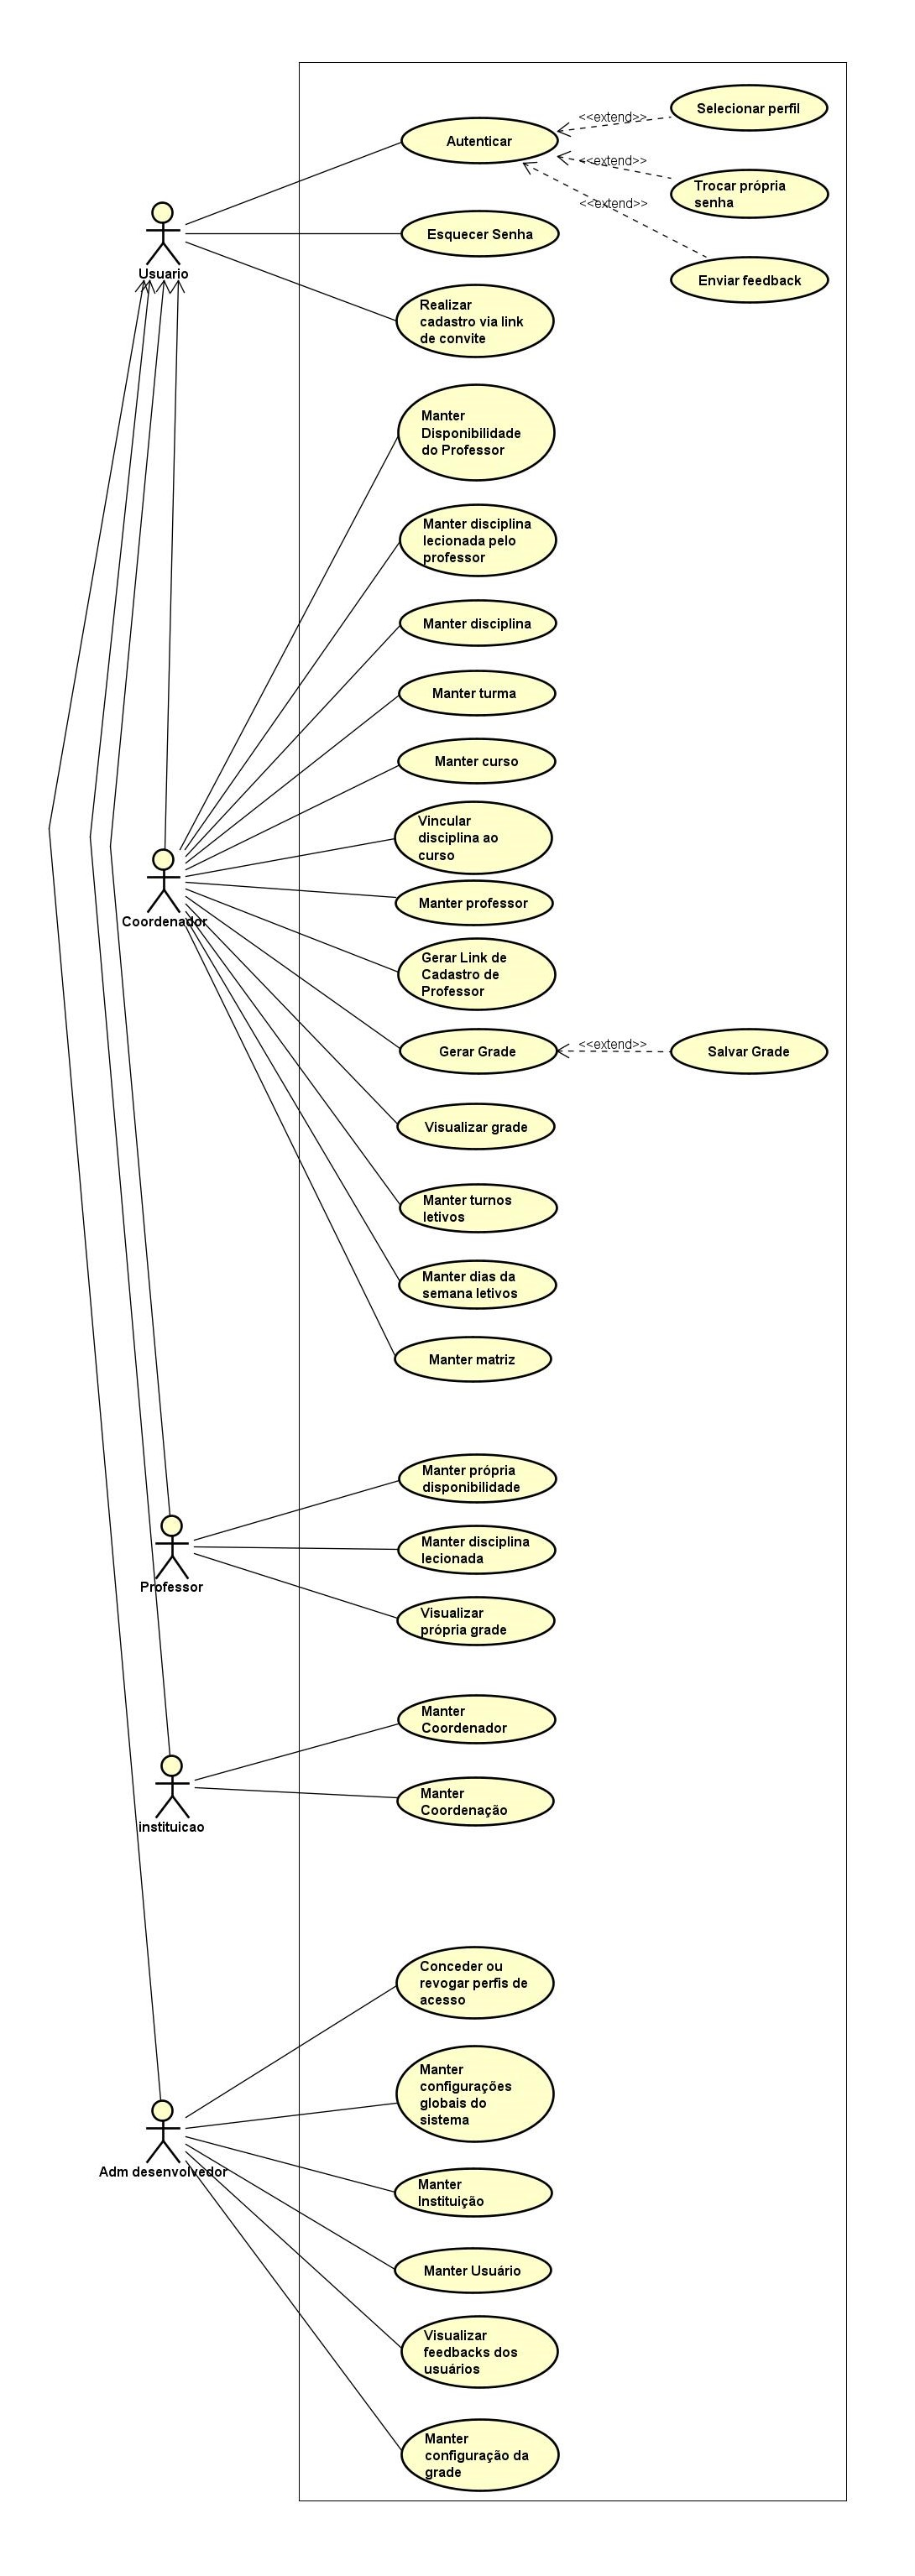
\includegraphics[width=\textwidth,height=0.86\textheight,keepaspectratio]{figuras/Figura_9_Diagrama de casos de uso.jpg}
\fonteautores
\end{figure}

\clearpage

\subsection{Descrição dos Casos de Uso}
\label{subsec:4.2.3}

Para eliminar ambiguidades inerentes à representação gráfica, os casos de uso foram detalhados textualmente seguindo o modelo de especificação padrão, com descrição, ator, pré-condição, pós-condição e fluxo principal de interação. Os Quadros de UC01 a UC33 apresentam a especificação completa de cada caso de uso do sistema.

% Tabela 3
\vspace{\baselineskip}

\Needspace{0.48\textheight}
\begin{longtable}{|L{4.5cm}|L{10.5cm}|}
\caption{Especificação do Caso de Uso: UC01 -- Autenticar} \\
\hline
\textbf{Nome do caso de uso} & \textbf{UC01 -- Autenticar} \\
\hline
\endfirsthead
\hline
\textbf{Nome do caso de uso} & \textbf{UC01 -- Autenticar} \\
\hline
\endhead
Descrição       & Permite que o usuário acesse o sistema de forma segura. \\
\hline
Ator            & Usuário \\
\hline
Pré-condição    & O usuário deve possuir um cadastro válido. \\
\hline
Pós-condição    & O usuário é logado no sistema e o token JWT é injetado. \\
\hline
Fluxo Principal & Ação do Ator: Informa login e senha e clica em entrar. Ação do Sistema: Valida credenciais no banco, gera o token de acesso e redireciona o usuário. \\
\hline
\end{longtable}

\fonteautores

% Tabela 4
\vspace{\baselineskip}

\Needspace{0.48\textheight}
\begin{longtable}{|L{4.5cm}|L{10.5cm}|}
\caption{Especificação do Caso de Uso: UC02 -- Selecionar/Trocar Perfil} \\
\hline
\textbf{Nome do caso de uso} & \textbf{UC02 -- Selecionar/Trocar Perfil} \\
\hline
\endfirsthead
\hline
\textbf{Nome do caso de uso} & \textbf{UC02 -- Selecionar/Trocar Perfil} \\
\hline
\endhead
Descrição       & Permite alterar o papel ativo na sessão (ex: trocar a visão de Professor para Coordenador). \\
\hline
Ator            & Usuário (Autenticado) \\
\hline
Pré-condição    & O usuário deve possuir múltiplos vínculos de perfis ativos. \\
\hline
Pós-condição    & O sistema reemite o token JWT com as permissões do novo perfil selecionado. \\
\hline
Fluxo Principal & Ação do Ator: Seleciona um novo perfil na interface e confirma. Ação do Sistema: Invalida o contexto anterior, emite novo token JWT e recarrega a página. \\
\hline
\end{longtable}

\fonteautores

% Tabela 5
\vspace{\baselineskip}

\Needspace{0.48\textheight}
\begin{longtable}{|L{4.5cm}|L{10.5cm}|}
\caption{Especificação do Caso de Uso: UC03 -- Trocar Própria Senha} \\
\hline
\textbf{Nome do caso de uso} & \textbf{UC03 -- Trocar Própria Senha} \\
\hline
\endfirsthead
\hline
\textbf{Nome do caso de uso} & \textbf{UC03 -- Trocar Própria Senha} \\
\hline
\endhead
Descrição       & Permite que o usuário altere sua senha por motivos de segurança. \\
\hline
Ator            & Usuário (Autenticado) \\
\hline
Pré-condição    & O usuário deve estar logado e saber sua senha atual. \\
\hline
Pós-condição    & A senha atual é substituída pela nova senha criptografada. \\
\hline
Fluxo Principal & Ação do Ator: Informa a senha atual e a nova senha desejada. Ação do Sistema: Valida a senha atual e criptografa e salva a nova. \\
\hline
\end{longtable}

\fonteautores

% Tabela 6
\vspace{\baselineskip}

\Needspace{0.48\textheight}
\begin{longtable}{|L{4.5cm}|L{10.5cm}|}
\caption{Especificação do Caso de Uso: UC04 -- Enviar Feedback} \\
\hline
\textbf{Nome do caso de uso} & \textbf{UC04 -- Enviar Feedback} \\
\hline
\endfirsthead
\hline
\textbf{Nome do caso de uso} & \textbf{UC04 -- Enviar Feedback} \\
\hline
\endhead
Descrição       & Enviar sugestões ou reportar bugs do sistema para os administradores. \\
\hline
Ator            & Usuário (Autenticado) \\
\hline
Pré-condição    & Estar logado no sistema. \\
\hline
Pós-condição    & O feedback é registrado na base atrelado ao usuário remetente. \\
\hline
Fluxo Principal & Ação do Ator: Seleciona a categoria, digita a mensagem e envia. Ação do Sistema: Salva o feedback no banco de dados. \\
\hline
\end{longtable}

\fonteautores

% Tabela 7
\vspace{\baselineskip}

\Needspace{0.48\textheight}
\begin{longtable}{|L{4.5cm}|L{10.5cm}|}
\caption{Especificação do Caso de Uso: UC05 -- Esquecer Senha} \\
\hline
\textbf{Nome do caso de uso} & \textbf{UC05 -- Esquecer Senha} \\
\hline
\endfirsthead
\hline
\textbf{Nome do caso de uso} & \textbf{UC05 -- Esquecer Senha} \\
\hline
\endhead
Descrição       & Permite ao usuário recuperar o acesso através de um link enviado por e-mail. \\
\hline
Ator            & Usuário \\
\hline
Pré-condição    & O usuário não consegue logar, mas possui acesso ao seu e-mail cadastrado. \\
\hline
Pós-condição    & Uma nova senha é cadastrada para o usuário. \\
\hline
Fluxo Principal & Ação do Ator: Solicita recuperação informando e-mail. Acessa o link e digita a nova senha. Ação do Sistema: Envia o e-mail com token. Valida o token e atualiza a senha no banco. \\
\hline
\end{longtable}

\fonteautores

% Tabela 8
\vspace{\baselineskip}

\Needspace{0.48\textheight}
\begin{longtable}{|L{4.5cm}|L{10.5cm}|}
\caption{Especificação do Caso de Uso: UC06 -- Realizar Cadastro via Link de Convite} \\
\hline
\textbf{Nome do caso de uso} & \textbf{UC06 -- Realizar Cadastro via Link de Convite} \\
\hline
\endfirsthead
\hline
\textbf{Nome do caso de uso} & \textbf{UC06 -- Realizar Cadastro via Link de Convite} \\
\hline
\endhead
Descrição       & Cadastro facilitado onde o professor já entra vinculado à faculdade. \\
\hline
Ator            & Usuário (Visitante/Professor) \\
\hline
Pré-condição    & Possuir um link/token de convite válido gerado por um coordenador. \\
\hline
Pós-condição    & Conta criada já com o perfil de Professor vinculado à instituição de origem do link. \\
\hline
Fluxo Principal & Ação do Ator: Acessa o link e preenche a senha e dados faltantes. Ação do Sistema: Valida o token do link, cria o usuário, atribui o perfil ACESSO\_PROFESSOR e expira o link. \\
\hline
\end{longtable}

\fonteautores

% Tabela 9
\vspace{\baselineskip}

\Needspace{0.48\textheight}
\begin{longtable}{|L{4.5cm}|L{10.5cm}|}
\caption{Especificação do Caso de Uso: UC07 -- Manter Disponibilidade do Professor} \\
\hline
\textbf{Nome do caso de uso} & \textbf{UC07 -- Manter Disponibilidade do Professor} \\
\hline
\endfirsthead
\hline
\textbf{Nome do caso de uso} & \textbf{UC07 -- Manter Disponibilidade do Professor} \\
\hline
\endhead
Descrição       & Permite ao coordenador visualizar e, se necessário, intervir na disponibilidade de tempo informada pelos professores. \\
\hline
Ator            & Coordenador \\
\hline
Pré-condição    & Professores devem possuir cadastro e vínculos na instituição. \\
\hline
Pós-condição    & A malha de disponibilidade dos professores fica pronta para o algoritmo. \\
\hline
Fluxo Principal & Ação do Ator: Consulta ou ajusta os dias/horários livres de um professor. Ação do Sistema: Salva a entidade Disponibilidade. \\
\hline
\end{longtable}

\fonteautores

% Tabela 10
\vspace{\baselineskip}

\Needspace{0.48\textheight}
\begin{longtable}{|L{4.5cm}|L{10.5cm}|}
\caption{Especificação do Caso de Uso: UC08 -- Manter Disciplina Lecionada pelo Professor} \\
\hline
\textbf{Nome do caso de uso} & \textbf{UC08 -- Manter Disciplina Lecionada pelo Professor} \\
\hline
\endfirsthead
\hline
\textbf{Nome do caso de uso} & \textbf{UC08 -- Manter Disciplina Lecionada pelo Professor} \\
\hline
\endhead
Descrição       & Permite ao coordenador gerenciar a equipe de professores e o que eles podem lecionar. \\
\hline
Ator            & Coordenador \\
\hline
Pré-condição    & Professores devem estar cadastrados na instituição. \\
\hline
Pós-condição    & Professor é mantido e vínculos com disciplinas são atualizados. \\
\hline
Fluxo Principal & Ação do Ator: Seleciona um professor e marca as disciplinas nas quais ele tem domínio. Ação do Sistema: Salva os registros na entidade UsuarioDisciplina. \\
\hline
\end{longtable}

\fonteautores

% Tabela 11
\vspace{\baselineskip}

\Needspace{0.48\textheight}
\begin{longtable}{|L{4.5cm}|L{10.5cm}|}
\caption{Especificação do Caso de Uso: UC09 -- Manter Disciplina} \\
\hline
\textbf{Nome do caso de uso} & \textbf{UC09 -- Manter Disciplina} \\
\hline
\endfirsthead
\hline
\textbf{Nome do caso de uso} & \textbf{UC09 -- Manter Disciplina} \\
\hline
\endhead
Descrição       & Permite gerenciar o catálogo global de disciplinas da coordenação. \\
\hline
Ator            & Coordenador \\
\hline
Pré-condição    & Estar logado como Coordenador. \\
\hline
Pós-condição    & A disciplina passa a existir no catálogo. \\
\hline
Fluxo Principal & Ação do Ator: Insere nome e carga horária da disciplina. Ação do Sistema: Persiste a disciplina no banco. \\
\hline
\end{longtable}

\fonteautores

% Tabela 12
\vspace{\baselineskip}

\Needspace{0.48\textheight}
\begin{longtable}{|L{4.5cm}|L{10.5cm}|}
\caption{Especificação do Caso de Uso: UC10 -- Manter Turma} \\
\hline
\textbf{Nome do caso de uso} & \textbf{UC10 -- Manter Turma} \\
\hline
\endfirsthead
\hline
\textbf{Nome do caso de uso} & \textbf{UC10 -- Manter Turma} \\
\hline
\endhead
Descrição       & Permite criar turmas de um curso para um determinado semestre/ano. \\
\hline
Ator            & Coordenador \\
\hline
Pré-condição    & Curso e Turno devem estar cadastrados. \\
\hline
Pós-condição    & Turma é instanciada e pronta para receber alunos/matrizes. \\
\hline
Fluxo Principal & Ação do Ator: Informa nome, curso, turno, semestre e ano. Ação do Sistema: Salva a entidade Turma vinculada à coordenação. \\
\hline
\end{longtable}

\fonteautores

% Tabela 13
\vspace{\baselineskip}

\Needspace{0.48\textheight}
\begin{longtable}{|L{4.5cm}|L{10.5cm}|}
\caption{Especificação do Caso de Uso: UC11 -- Manter Curso} \\
\hline
\textbf{Nome do caso de uso} & \textbf{UC11 -- Manter Curso} \\
\hline
\endfirsthead
\hline
\textbf{Nome do caso de uso} & \textbf{UC11 -- Manter Curso} \\
\hline
\endhead
Descrição       & Permite gerenciar os cursos oferecidos pela coordenação. \\
\hline
Ator            & Coordenador \\
\hline
Pré-condição    & Estar logado com o perfil de Coordenador. \\
\hline
Pós-condição    & Curso é criado, alterado ou removido logicamente. \\
\hline
Fluxo Principal & Ação do Ator: Preenche os dados do curso e solicita salvar. Ação do Sistema: Valida os dados e salva o curso atrelado à instituição/coordenação. \\
\hline
\end{longtable}

\fonteautores

% Tabela 14
\vspace{\baselineskip}

\Needspace{0.48\textheight}
\begin{longtable}{|L{4.5cm}|L{10.5cm}|}
\caption{Especificação do Caso de Uso: UC12 -- Vincular Disciplina ao Curso} \\
\hline
\textbf{Nome do caso de uso} & \textbf{UC12 -- Vincular Disciplina ao Curso} \\
\hline
\endfirsthead
\hline
\textbf{Nome do caso de uso} & \textbf{UC12 -- Vincular Disciplina ao Curso} \\
\hline
\endhead
Descrição       & Permite definir quais disciplinas fazem parte do catálogo de um curso. \\
\hline
Ator            & Coordenador \\
\hline
Pré-condição    & Curso e Disciplina devem existir. \\
\hline
Pós-condição    & Criado o relacionamento na tabela DisciplinaCurso. \\
\hline
Fluxo Principal & Ação do Ator: Seleciona o curso e marca as disciplinas pertencentes a ele. Ação do Sistema: Salva os vínculos na tabela de junção. \\
\hline
\end{longtable}

\fonteautores

% Tabela 15
\vspace{\baselineskip}

\Needspace{0.48\textheight}
\begin{longtable}{|L{4.5cm}|L{10.5cm}|}
\caption{Especificação do Caso de Uso: UC13 -- Manter Professor} \\
\hline
\textbf{Nome do caso de uso} & \textbf{UC13 -- Manter Professor} \\
\hline
\endfirsthead
\hline
\textbf{Nome do caso de uso} & \textbf{UC13 -- Manter Professor} \\
\hline
\endhead
Descrição       & Permite gerenciar os dados cadastrais básicos dos professores da instituição. \\
\hline
Ator            & Coordenador \\
\hline
Pré-condição    & Ter permissão de Coordenador. \\
\hline
Pós-condição    & Dados do professor são atualizados/cadastrados. \\
\hline
Fluxo Principal & Ação do Ator: Altera informações do professor. Ação do Sistema: Atualiza o cadastro no banco. \\
\hline
\end{longtable}

\fonteautores

% Tabela 16
\vspace{\baselineskip}

\Needspace{0.48\textheight}
\begin{longtable}{|L{4.5cm}|L{10.5cm}|}
\caption{Especificação do Caso de Uso: UC14 -- Gerar Link de Cadastro de Professor} \\
\hline
\textbf{Nome do caso de uso} & \textbf{UC14 -- Gerar Link de Cadastro de Professor} \\
\hline
\endfirsthead
\hline
\textbf{Nome do caso de uso} & \textbf{UC14 -- Gerar Link de Cadastro de Professor} \\
\hline
\endhead
Descrição       & Gera uma URL temporária criptografada para enviar a novos professores. \\
\hline
Ator            & Coordenador \\
\hline
Pré-condição    & Estar logado como coordenador da instituição. \\
\hline
Pós-condição    & Um link com token é gerado e retornado na tela. \\
\hline
Fluxo Principal & Ação do Ator: Clica no botão de gerar convite. Ação do Sistema: Cria um token seguro na entidade Link e exibe a URL. \\
\hline
\end{longtable}

\fonteautores

% Tabela 17
\vspace{\baselineskip}

\Needspace{0.48\textheight}
\begin{longtable}{|L{4.5cm}|L{10.5cm}|}
\caption{Especificação do Caso de Uso: UC15 -- Validar Usuários Cadastrados via Link} \\
\hline
\textbf{Nome do caso de uso} & \textbf{UC15 -- Validar Usuários Cadastrados via Link} \\
\hline
\endfirsthead
\hline
\textbf{Nome do caso de uso} & \textbf{UC15 -- Validar Usuários Cadastrados via Link} \\
\hline
\endhead
Descrição       & Permite ao coordenador aprovar ou rejeitar o acesso de professores que se cadastraram via link. \\
\hline
Ator            & Coordenador \\
\hline
Pré-condição    & Um professor deve ter concluído o cadastro através do link gerado. \\
\hline
Pós-condição    & O acesso do usuário é ativado ou desativado no sistema. \\
\hline
Fluxo Principal & Ação do Ator: Visualiza a lista de novos cadastros e altera o status para ativo ou inativo. Ação do Sistema: Atualiza a permissão de acesso do usuário no banco. \\
\hline
\end{longtable}

\fonteautores

% Tabela 18
\vspace{\baselineskip}

\Needspace{0.48\textheight}
\begin{longtable}{|L{4.5cm}|L{10.5cm}|}
\caption{Especificação do Caso de Uso: UC16 -- Gerar Grade} \\
\hline
\textbf{Nome do caso de uso} & \textbf{UC16 -- Gerar Grade} \\
\hline
\endfirsthead
\hline
\textbf{Nome do caso de uso} & \textbf{UC16 -- Gerar Grade} \\
\hline
\endhead
Descrição       & Aciona o algoritmo para montar o horário das turmas automaticamente. \\
\hline
Ator            & Coordenador \\
\hline
Pré-condição    & Turmas, professores, disciplinas (matrizes) e disponibilidades devem estar cadastradas. \\
\hline
Pós-condição    & Uma nova grade sugerida é retornada pelos microservices. \\
\hline
Fluxo Principal & Ação do Ator: Informa semestre/ano e clica em Gerar. Ação do Sistema: Envia os dados para os microservices (Sunny/Morpheus) e retorna a grade. \\
\hline
\end{longtable}

\fonteautores

% Tabela 19
\vspace{\baselineskip}

\Needspace{0.48\textheight}
\begin{longtable}{|L{4.5cm}|L{10.5cm}|}
\caption{Especificação do Caso de Uso: UC17 -- Salvar Grade} \\
\hline
\textbf{Nome do caso de uso} & \textbf{UC17 -- Salvar Grade} \\
\hline
\endfirsthead
\hline
\textbf{Nome do caso de uso} & \textbf{UC17 -- Salvar Grade} \\
\hline
\endhead
Descrição       & Efetiva a grade gerada ou manipulada manualmente no banco de dados. \\
\hline
Ator            & Coordenador \\
\hline
Pré-condição    & Uma grade válida deve estar em tela (Gerar Grade). \\
\hline
Pós-condição    & As alocações são persistidas e grades anteriores são arquivadas. \\
\hline
Fluxo Principal & Ação do Ator: Confirma as alocações e clica em Salvar. Ação do Sistema: Salva a nova entidade Grade e suas Alocacoes. \\
\hline
\end{longtable}

\fonteautores

% Tabela 20
\vspace{\baselineskip}

\Needspace{0.48\textheight}
\begin{longtable}{|L{4.5cm}|L{10.5cm}|}
\caption{Especificação do Caso de Uso: UC18 -- Visualizar Grade} \\
\hline
\textbf{Nome do caso de uso} & \textbf{UC18 -- Visualizar Grade} \\
\hline
\endfirsthead
\hline
\textbf{Nome do caso de uso} & \textbf{UC18 -- Visualizar Grade} \\
\hline
\endhead
Descrição       & Consultar a grade atualizada do semestre em vigor ou o histórico. \\
\hline
Ator            & Coordenador \\
\hline
Pré-condição    & A grade deve ter sido gerada e salva previamente. \\
\hline
Pós-condição    & O cronograma é exibido em formato de calendário/tabela. \\
\hline
Fluxo Principal & Ação do Ator: Seleciona o semestre/ano desejado. Ação do Sistema: Busca a Grade ativa e a exibe renderizada por turmas. \\
\hline
\end{longtable}

\fonteautores

% Tabela 21
\vspace{\baselineskip}

\Needspace{0.48\textheight}
\begin{longtable}{|L{4.5cm}|L{10.5cm}|}
\caption{Especificação do Caso de Uso: UC19 -- Manter Turnos Letivos} \\
\hline
\textbf{Nome do caso de uso} & \textbf{UC19 -- Manter Turnos Letivos} \\
\hline
\endfirsthead
\hline
\textbf{Nome do caso de uso} & \textbf{UC19 -- Manter Turnos Letivos} \\
\hline
\endhead
Descrição       & Gerenciar os turnos disponíveis (Matutino, Vespertino, Noturno). \\
\hline
Ator            & Coordenador \\
\hline
Pré-condição    & Estar logado como Coordenador. \\
\hline
Pós-condição    & Turnos são atualizados para uso. \\
\hline
Fluxo Principal & Ação do Ator: Adiciona ou altera nomes/horários de turnos. Ação do Sistema: Atualiza a entidade Turno. \\
\hline
\end{longtable}

\fonteautores

% Tabela 22
\vspace{\baselineskip}

\Needspace{0.48\textheight}
\begin{longtable}{|L{4.5cm}|L{10.5cm}|}
\caption{Especificação do Caso de Uso: UC20 -- Manter Dias da Semana Letivos} \\
\hline
\textbf{Nome do caso de uso} & \textbf{UC20 -- Manter Dias da Semana Letivos} \\
\hline
\endfirsthead
\hline
\textbf{Nome do caso de uso} & \textbf{UC20 -- Manter Dias da Semana Letivos} \\
\hline
\endhead
Descrição       & Gerenciar quais dias da semana ocorrem aulas na coordenação. \\
\hline
Ator            & Coordenador \\
\hline
Pré-condição    & Estar logado como Coordenador. \\
\hline
Pós-condição    & Dias úteis são atualizados para uso. \\
\hline
Fluxo Principal & Ação do Ator: Adiciona ou altera dias da semana. Ação do Sistema: Atualiza a entidade DiaSemana. \\
\hline
\end{longtable}

\fonteautores

% Tabela 23
\vspace{\baselineskip}

\Needspace{0.48\textheight}
\begin{longtable}{|L{4.5cm}|L{10.5cm}|}
\caption{Especificação do Caso de Uso: UC21 -- Manter Matriz} \\
\hline
\textbf{Nome do caso de uso} & \textbf{UC21 -- Manter Matriz} \\
\hline
\endfirsthead
\hline
\textbf{Nome do caso de uso} & \textbf{UC21 -- Manter Matriz} \\
\hline
\endhead
Descrição       & Permite vincular as disciplinas que uma turma específica terá em um determinado semestre. \\
\hline
Ator            & Coordenador \\
\hline
Pré-condição    & A Turma e as Disciplinas devem estar cadastradas. \\
\hline
Pós-condição    & O vínculo (Matriz) é salvo, servindo de base para o algoritmo gerar a grade. \\
\hline
Fluxo Principal & Ação do Ator: Seleciona uma turma e escolhe as disciplinas que comporão o semestre dela. Ação do Sistema: Salva os registros na entidade Matriz. \\
\hline
\end{longtable}

\fonteautores

% Tabela 24
\vspace{\baselineskip}

\Needspace{0.48\textheight}
\begin{longtable}{|L{4.5cm}|L{10.5cm}|}
\caption{Especificação do Caso de Uso: UC22 -- Manter Própria Disponibilidade} \\
\hline
\textbf{Nome do caso de uso} & \textbf{UC22 -- Manter Própria Disponibilidade} \\
\hline
\endfirsthead
\hline
\textbf{Nome do caso de uso} & \textbf{UC22 -- Manter Própria Disponibilidade} \\
\hline
\endhead
Descrição       & Informar à coordenação quais dias e turnos o professor tem horário livre para dar aula. \\
\hline
Ator            & Professor \\
\hline
Pré-condição    & Estar logado com o perfil de Professor. \\
\hline
Pós-condição    & A disponibilidade do semestre é salva no banco. \\
\hline
Fluxo Principal & Ação do Ator: Seleciona ano/semestre e marca em uma grade os horários livres. Ação do Sistema: Verifica duplicidades e salva as opções em Disponibilidade. \\
\hline
\end{longtable}

\fonteautores

% Tabela 25
\vspace{\baselineskip}

\Needspace{0.48\textheight}
\begin{longtable}{|L{4.5cm}|L{10.5cm}|}
\caption{Especificação do Caso de Uso: UC23 -- Manter Disciplina Lecionada} \\
\hline
\textbf{Nome do caso de uso} & \textbf{UC23 -- Manter Disciplina Lecionada} \\
\hline
\endfirsthead
\hline
\textbf{Nome do caso de uso} & \textbf{UC23 -- Manter Disciplina Lecionada} \\
\hline
\endhead
Descrição       & Visualizar quais disciplinas o coordenador vinculou ao seu perfil, ou solicitar alterações. \\
\hline
Ator            & Professor \\
\hline
Pré-condição    & Ter perfil de professor. \\
\hline
Pós-condição    & Exibe a lista de disciplinas atribuídas a ele. \\
\hline
Fluxo Principal & Ação do Ator: Acessa a tela de currículo/disciplinas. Ação do Sistema: Busca e lista as disciplinas da entidade UsuarioDisciplina. \\
\hline
\end{longtable}

\fonteautores

% Tabela 26
\vspace{\baselineskip}

\Needspace{0.48\textheight}
\begin{longtable}{|L{4.5cm}|L{10.5cm}|}
\caption{Especificação do Caso de Uso: UC24 -- Visualizar Própria Grade} \\
\hline
\textbf{Nome do caso de uso} & \textbf{UC24 -- Visualizar Própria Grade} \\
\hline
\endfirsthead
\hline
\textbf{Nome do caso de uso} & \textbf{UC24 -- Visualizar Própria Grade} \\
\hline
\endhead
Descrição       & Consultar seu próprio cronograma de aulas na semana. \\
\hline
Ator            & Professor \\
\hline
Pré-condição    & A grade do semestre deve estar finalizada e salva pelo coordenador. \\
\hline
Pós-condição    & Exibe apenas as alocações que o envolvem. \\
\hline
Fluxo Principal & Ação do Ator: Acessa a visualização de horários. Ação do Sistema: Filtra a Grade ativa buscando apenas alocações vinculadas ao seu ID e exibe. \\
\hline
\end{longtable}

\fonteautores

% Tabela 27
\vspace{\baselineskip}

\Needspace{0.48\textheight}
\begin{longtable}{|L{4.5cm}|L{10.5cm}|}
\caption{Especificação do Caso de Uso: UC25 -- Manter Coordenador} \\
\hline
\textbf{Nome do caso de uso} & \textbf{UC25 -- Manter Coordenador} \\
\hline
\endfirsthead
\hline
\textbf{Nome do caso de uso} & \textbf{UC25 -- Manter Coordenador} \\
\hline
\endhead
Descrição       & Atribuir ou remover o cargo de coordenação a usuários. \\
\hline
Ator            & Adm Instituição \\
\hline
Pré-condição    & O usuário a ser promovido já deve estar cadastrado. \\
\hline
Pós-condição    & O usuário ganha o perfil ACESSO\_COORDENADOR. \\
\hline
Fluxo Principal & Ação do Ator: Seleciona um usuário e o vincula a uma Coordenação específica. Ação do Sistema: Cria o vínculo UsuarioPerfil e CoordenacaoVinculo. \\
\hline
\end{longtable}

\fonteautores

% Tabela 28
\vspace{\baselineskip}

\Needspace{0.48\textheight}
\begin{longtable}{|L{4.5cm}|L{10.5cm}|}
\caption{Especificação do Caso de Uso: UC26 -- Manter Coordenação} \\
\hline
\textbf{Nome do caso de uso} & \textbf{UC26 -- Manter Coordenação} \\
\hline
\endfirsthead
\hline
\textbf{Nome do caso de uso} & \textbf{UC26 -- Manter Coordenação} \\
\hline
\endhead
Descrição       & Gerenciar quais polos ou departamentos de coordenação existem na faculdade. \\
\hline
Ator            & Adm Instituição \\
\hline
Pré-condição    & Ter permissão ACESSO\_ADMIN\_INSTITUICAO. \\
\hline
Pós-condição    & Coordenações são adicionadas ou editadas na Instituição. \\
\hline
Fluxo Principal & Ação do Ator: Informa o nome do departamento e salva. Ação do Sistema: Salva a entidade Coordenacao vinculada à Instituicao. \\
\hline
\end{longtable}

\fonteautores

% Tabela 29
\vspace{\baselineskip}

\Needspace{0.48\textheight}
\begin{longtable}{|L{4.5cm}|L{10.5cm}|}
\caption{Especificação do Caso de Uso: UC27 -- Conceder ou Revogar Perfis de Acesso} \\
\hline
\textbf{Nome do caso de uso} & \textbf{UC27 -- Conceder ou Revogar Perfis de Acesso} \\
\hline
\endfirsthead
\hline
\textbf{Nome do caso de uso} & \textbf{UC27 -- Conceder ou Revogar Perfis de Acesso} \\
\hline
\endhead
Descrição       & Gerenciar dinamicamente quais perfis (Professor, etc.) os usuários da instituição possuem. \\
\hline
Ator            & Adm Instituição \\
\hline
Pré-condição    & Ter permissão ACESSO\_ADMIN\_INSTITUICAO. \\
\hline
Pós-condição    & Perfis são atualizados no banco para o usuário selecionado. \\
\hline
Fluxo Principal & Ação do Ator: Seleciona o usuário e adiciona ou retira permissões. Ação do Sistema: Atualiza a tabela de junção UsuarioPerfil. \\
\hline
\end{longtable}

\fonteautores

% Tabela 30
\vspace{\baselineskip}

\Needspace{0.48\textheight}
\begin{longtable}{|L{4.5cm}|L{10.5cm}|}
\caption{Especificação do Caso de Uso: UC28 -- Manter Configurações da Faculdade} \\
\hline
\textbf{Nome do caso de uso} & \textbf{UC28 -- Manter Configurações da Faculdade} \\
\hline
\endfirsthead
\hline
\textbf{Nome do caso de uso} & \textbf{UC28 -- Manter Configurações da Faculdade} \\
\hline
\endhead
Descrição       & Alterar parâmetros locais da faculdade, como restrições de horários institucionais. \\
\hline
Ator            & Adm Instituição \\
\hline
Pré-condição    & Ter permissão ACESSO\_ADMIN\_INSTITUICAO. \\
\hline
Pós-condição    & A entidade ConfigFaculdade é atualizada. \\
\hline
Fluxo Principal & Ação do Ator: Altera parâmetros no painel de configurações. Ação do Sistema: Persiste as opções no banco. \\
\hline
\end{longtable}

\fonteautores

% Tabela 31
\vspace{\baselineskip}

\Needspace{0.48\textheight}
\begin{longtable}{|L{4.5cm}|L{10.5cm}|}
\caption{Especificação do Caso de Uso: UC29 -- Manter Configurações Globais do Sistema} \\
\hline
\textbf{Nome do caso de uso} & \textbf{UC29 -- Manter Configurações Globais do Sistema} \\
\hline
\endfirsthead
\hline
\textbf{Nome do caso de uso} & \textbf{UC29 -- Manter Configurações Globais do Sistema} \\
\hline
\endhead
Descrição       & Alterar hiperparâmetros matemáticos dos microservices e variáveis do sistema (Modo Manutenção). \\
\hline
Ator            & Adm Desenvolvedor \\
\hline
Pré-condição    & Estar autenticado como ACESSO\_ADMIN. \\
\hline
Pós-condição    & Variáveis em banco e em memória de Cache são atualizadas em tempo real. \\
\hline
Fluxo Principal & Ação do Ator: Acessa o painel Dinâmico e altera parâmetros (tamanho da população, número de gerações, taxa de \textit{crossover}, taxa de mutação, taxa de elitismo, tamanho do torneio, penalidade de conflito, pontuação base, bônus de diversidade). Ação do Sistema: Salva na entidade ConfigSistema e limpa o cache. \\
\hline
\end{longtable}

\fonteautores

% Tabela 32
\vspace{\baselineskip}

\Needspace{0.48\textheight}
\begin{longtable}{|L{4.5cm}|L{10.5cm}|}
\caption{Especificação do Caso de Uso: UC30 -- Manter Instituição} \\
\hline
\textbf{Nome do caso de uso} & \textbf{UC30 -- Manter Instituição} \\
\hline
\endfirsthead
\hline
\textbf{Nome do caso de uso} & \textbf{UC30 -- Manter Instituição} \\
\hline
\endhead
Descrição       & Cadastrar e gerenciar novas Universidades ou Faculdades (clientes) no sistema. \\
\hline
Ator            & Adm Desenvolvedor \\
\hline
Pré-condição    & Estar autenticado como ACESSO\_ADMIN. \\
\hline
Pós-condição    & Uma nova Instituição passa a existir e poder comportar usuários. \\
\hline
Fluxo Principal & Ação do Ator: Insere nome, dados da Instituição. Ação do Sistema: Salva a entidade Instituicao. \\
\hline
\end{longtable}

\fonteautores

% Tabela 33
\vspace{\baselineskip}

\Needspace{0.48\textheight}
\begin{longtable}{|L{4.5cm}|L{10.5cm}|}
\caption{Especificação do Caso de Uso: UC31 -- Manter Usuário} \\
\hline
\textbf{Nome do caso de uso} & \textbf{UC31 -- Manter Usuário} \\
\hline
\endfirsthead
\hline
\textbf{Nome do caso de uso} & \textbf{UC31 -- Manter Usuário} \\
\hline
\endhead
Descrição       & Gerenciamento global e absoluto de todos os usuários cadastrados. \\
\hline
Ator            & Adm Desenvolvedor \\
\hline
Pré-condição    & Estar autenticado como ACESSO\_ADMIN. \\
\hline
Pós-condição    & Contas podem ser suspensas, editadas ou removidas. \\
\hline
Fluxo Principal & Ação do Ator: Consulta a base completa de usuários e aplica edições. Ação do Sistema: Atualiza o registro do usuário na base. \\
\hline
\end{longtable}

\fonteautores

% Tabela 34
\vspace{\baselineskip}

\Needspace{0.48\textheight}
\begin{longtable}{|L{4.5cm}|L{10.5cm}|}
\caption{Especificação do Caso de Uso: UC32 -- Manter Perfis de Acesso do Sistema} \\
\hline
\textbf{Nome do caso de uso} & \textbf{UC32 -- Manter Perfis de Acesso do Sistema} \\
\hline
\endfirsthead
\hline
\textbf{Nome do caso de uso} & \textbf{UC32 -- Manter Perfis de Acesso do Sistema} \\
\hline
\endhead
Descrição       & Gerenciar os papéis fundamentais (Roles) e privilégios disponíveis no sistema. \\
\hline
Ator            & Adm Desenvolvedor \\
\hline
Pré-condição    & Estar autenticado como ACESSO\_ADMIN. \\
\hline
Pós-condição    & Permissões globais são alteradas. \\
\hline
Fluxo Principal & Ação do Ator: Edita perfis de acesso nativos. Ação do Sistema: Atualiza a entidade Perfil na base. \\
\hline
\end{longtable}

\fonteautores

% Tabela 35
\vspace{\baselineskip}

\Needspace{0.48\textheight}
\begin{longtable}{|L{4.5cm}|L{10.5cm}|}
\caption{Especificação do Caso de Uso: UC33 -- Visualizar Feedbacks dos Usuários} \\
\hline
\textbf{Nome do caso de uso} & \textbf{UC33 -- Visualizar Feedbacks dos Usuários} \\
\hline
\endfirsthead
\hline
\textbf{Nome do caso de uso} & \textbf{UC33 -- Visualizar Feedbacks dos Usuários} \\
\hline
\endhead
Descrição       & Ler relatórios de erros/sugestões enviados por usuários e gerenciar o fluxo de chamados. \\
\hline
Ator            & Adm Desenvolvedor \\
\hline
Pré-condição    & Estar autenticado como ACESSO\_ADMIN. \\
\hline
Pós-condição    & Feedback é lido/arquivado e ações tomadas. \\
\hline
Fluxo Principal & Ação do Ator: Acessa a caixa de feedback recebida. Ação do Sistema: Consulta e exibe as listagens de Feedback da base. \\
\hline
\end{longtable}

\fonteautores

% Chapter 5

\section{Modelagem Estrutural}
\label{sec:4.3}

A modelagem estrutural descreve a organização estática do sistema por meio das classes, seus atributos, métodos e relacionamentos. \citeonline{fowler2004} destaca que o diagrama de classes não se limita à listagem de atributos, mas expressa a estrutura estática do sistema e as relações entre suas entidades, funcionando como base para a organização do modelo.

\subsection{Diagrama de Classes}
\label{subsec:4.3.1}

O Diagrama de Classes do IGRIS apresenta a estrutura completa das entidades de domínio e seus relacionamentos. A organização reflete diretamente os módulos do backend: controle de acesso, domínio acadêmico e núcleo de otimização.

O controle de acesso é sustentado pela entidade \texttt{UsuarioPerfil}, que implementa o padrão de múltiplos perfis por usuário; um mesmo colaborador pode exercer simultaneamente as funções de professor e coordenador sem duplicação de cadastro. As entidades \texttt{Perfil}, \texttt{Link} e \texttt{TipoLink} complementam esse módulo, gerenciando permissões e o mecanismo de convite por link.

No domínio acadêmico, a classe \texttt{Curso} atua como agregadora principal, relacionando-se com \texttt{Disciplina} por meio de \texttt{DisciplinaCurso} para compor a matriz curricular, e com \texttt{Turma} para definir as ofertas semestrais. A entidade \texttt{Matriz} vincula turmas e disciplinas em um semestre específico, representando a grade curricular que alimenta o algoritmo genético. A tabela \texttt{UsuarioDisciplina} mapeia quais professores estão aptos a ministrar cada disciplina.

O núcleo do sistema é a entidade \texttt{AlocacaoGrade}, que materializa a solução do problema de timetabling ao vincular uma matriz, uma disponibilidade, uma grade e um usuário docente. Cada instância dessa entidade representa o resultado do algoritmo genético ao reunir simultaneamente a disponibilidade do professor, a necessidade da turma e a restrição de horário.

\begin{landscape}
\begin{figure}[p]
\centering
\caption{Diagrama de Classes do IGRIS}
\label{fig:diagrama_classes}
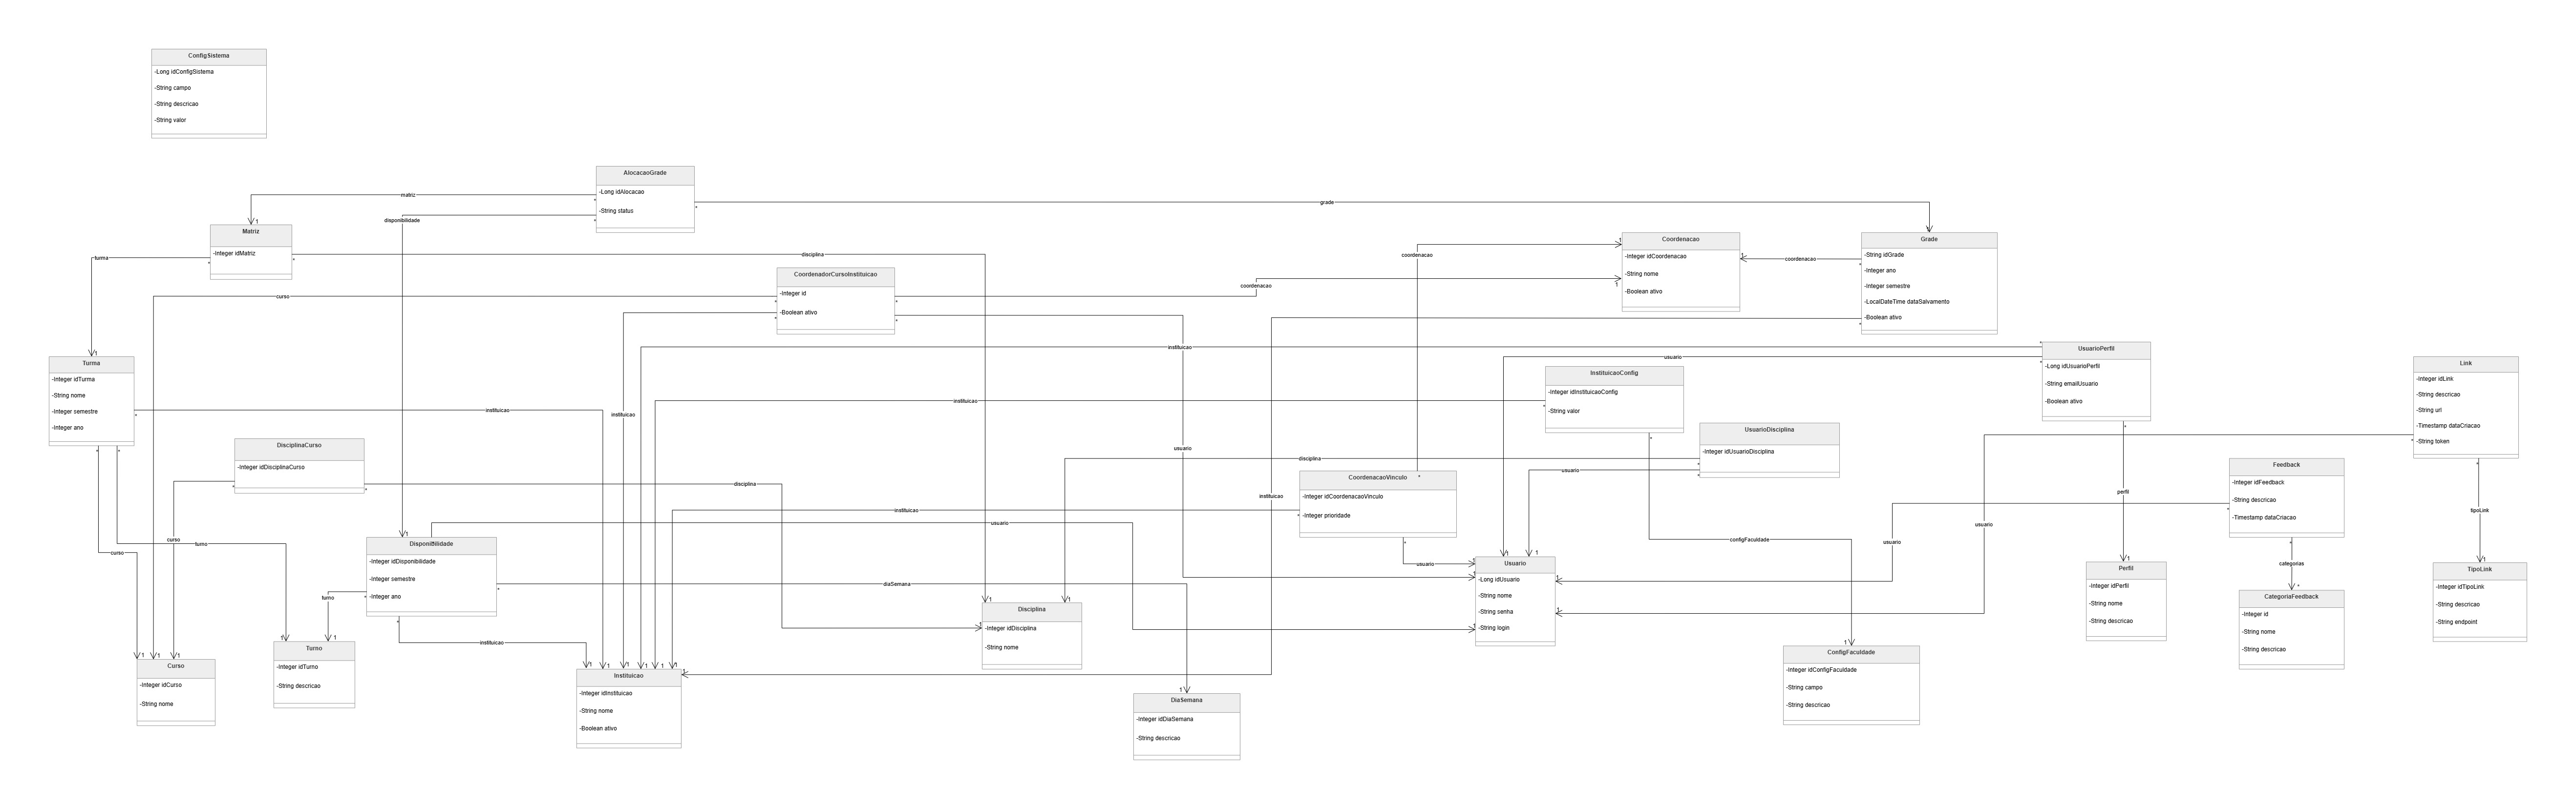
\includegraphics[width=\linewidth,height=0.9\textheight,keepaspectratio]{figuras/Figura_10_diagrama de classe.jpg}
\fonteautores
\end{figure}
\end{landscape}

\subsection{Especificação das Classes}
\label{subsec:4.3.2}

As tabelas a seguir descrevem os atributos, tipos de dados, visibilidade e semântica de cada classe identificada no modelo orientado a objetos do IGRIS, servindo como referência para a implementação das entidades de domínio.

% Tabela 64
\vspace{\baselineskip}

\Needspace{0.32\textheight}
\begin{longtable}{|L{3.5cm}|L{3.5cm}|L{3.5cm}|L{3.5cm}|}
\caption{Especificação da Classe: Instituicao} \\
\hline
\textbf{Elemento} & \textbf{Tipo/Assinatura} & \textbf{Visibilidade} & \textbf{Descrição} \\
\hline
\endfirsthead
\hline
\textbf{Elemento} & \textbf{Tipo/Assinatura} & \textbf{Visibilidade} & \textbf{Descrição} \\
\hline
\endhead
idInstituicao & int & private & Identificador único da instituição. \\
\hline
nome & String & private & Nome oficial da instituição. \\
\hline
ativo & boolean & private & Indicador se a instituição está ativa no sistema. \\
\hline
\end{longtable}

\fonteautores

% Tabela 65
\vspace{\baselineskip}

\Needspace{0.32\textheight}
\begin{longtable}{|L{3.5cm}|L{3.5cm}|L{3.5cm}|L{3.5cm}|}
\caption{Especificação da Classe: Coordenacao} \\
\hline
\textbf{Elemento} & \textbf{Tipo/Assinatura} & \textbf{Visibilidade} & \textbf{Descrição} \\
\hline
\endfirsthead
\hline
\textbf{Elemento} & \textbf{Tipo/Assinatura} & \textbf{Visibilidade} & \textbf{Descrição} \\
\hline
\endhead
idCoordenacao & int & private & Identificador da coordenação. \\
\hline
nome & String & private & Nome da coordenação (ex.: Engenharia de Software). \\
\hline
ativo & boolean & private & Indica se a coordenação está ativa. \\
\hline
instituicao & Instituicao & private & Instituição a que a coordenação pertence. \\
\hline
\end{longtable}

\fonteautores

% Tabela 66
\vspace{\baselineskip}

\Needspace{0.32\textheight}
\begin{longtable}{|L{3.5cm}|L{3.5cm}|L{3.5cm}|L{3.5cm}|}
\caption{Especificação da Classe: CoordenadorCursoInstituicao} \\
\hline
\textbf{Elemento} & \textbf{Tipo/Assinatura} & \textbf{Visibilidade} & \textbf{Descrição} \\
\hline
\endfirsthead
\hline
\textbf{Elemento} & \textbf{Tipo/Assinatura} & \textbf{Visibilidade} & \textbf{Descrição} \\
\hline
\endhead
idCoordenadorCurso & int & private & Identificador do vínculo do coordenador ao curso/instituição. \\
\hline
coordenacao & Coordenacao & private & Coordenação associada. \\
\hline
usuario & Usuario & private & Usuário que atua como coordenador. \\
\hline
instituicao & Instituicao & private & Instituição do vínculo. \\
\hline
curso & Curso & private & Curso coordenado. \\
\hline
\end{longtable}

\fonteautores

% Tabela 67
\vspace{\baselineskip}

\Needspace{0.32\textheight}
\begin{longtable}{|L{3.5cm}|L{3.5cm}|L{3.5cm}|L{3.5cm}|}
\caption{Especificação da Classe: CoordenacaoVinculo} \\
\hline
\textbf{Elemento} & \textbf{Tipo/Assinatura} & \textbf{Visibilidade} & \textbf{Descrição} \\
\hline
\endfirsthead
\hline
\textbf{Elemento} & \textbf{Tipo/Assinatura} & \textbf{Visibilidade} & \textbf{Descrição} \\
\hline
\endhead
usuario & Usuario & private & Usuário vinculado à coordenação. \\
\hline
coordenacao & Coordenacao & private & Coordenação vinculada. \\
\hline
instituicao & Instituicao & private & Instituição do vínculo. \\
\hline
prioridade & int & private & Prioridade do vínculo, usada para resolução de conflitos. \\
\hline
\end{longtable}

\fonteautores

% Tabela 68
\vspace{\baselineskip}

\Needspace{0.32\textheight}
\begin{longtable}{|L{3.5cm}|L{3.5cm}|L{3.5cm}|L{3.5cm}|}
\caption{Especificação da Classe: Curso} \\
\hline
\textbf{Elemento} & \textbf{Tipo/Assinatura} & \textbf{Visibilidade} & \textbf{Descrição} \\
\hline
\endfirsthead
\hline
\textbf{Elemento} & \textbf{Tipo/Assinatura} & \textbf{Visibilidade} & \textbf{Descrição} \\
\hline
\endhead
idCurso & int & private & Identificador do curso. \\
\hline
nome & String & private & Nome do curso (ex.: Ciência da Computação). \\
\hline
\end{longtable}

\fonteautores

% Tabela 69
\vspace{\baselineskip}

\Needspace{0.32\textheight}
\begin{longtable}{|L{3.5cm}|L{3.5cm}|L{3.5cm}|L{3.5cm}|}
\caption{Especificação da Classe: Disciplina} \\
\hline
\textbf{Elemento} & \textbf{Tipo/Assinatura} & \textbf{Visibilidade} & \textbf{Descrição} \\
\hline
\endfirsthead
\hline
\textbf{Elemento} & \textbf{Tipo/Assinatura} & \textbf{Visibilidade} & \textbf{Descrição} \\
\hline
\endhead
idDisciplina & int & private & Identificador da disciplina. \\
\hline
nome & String & private & Nome da disciplina. \\
\hline
\end{longtable}

\fonteautores

% Tabela 70
\vspace{\baselineskip}

\Needspace{0.32\textheight}
\begin{longtable}{|L{3.5cm}|L{3.5cm}|L{3.5cm}|L{3.5cm}|}
\caption{Especificação da Classe: DisciplinaCurso} \\
\hline
\textbf{Elemento} & \textbf{Tipo/Assinatura} & \textbf{Visibilidade} & \textbf{Descrição} \\
\hline
\endfirsthead
\hline
\textbf{Elemento} & \textbf{Tipo/Assinatura} & \textbf{Visibilidade} & \textbf{Descrição} \\
\hline
\endhead
idDisciplinaCurso & int & private & Identificador da associação disciplina-curso. \\
\hline
curso & Curso & private & Curso ao qual a disciplina pertence. \\
\hline
disciplina & Disciplina & private & Disciplina associada. \\
\hline
semestre & int & private & Semestre previsto na matriz curricular (quando aplicável). \\
\hline
\end{longtable}

\fonteautores

% Tabela 71
\vspace{\baselineskip}

\Needspace{0.32\textheight}
\begin{longtable}{|L{3.5cm}|L{3.5cm}|L{3.5cm}|L{3.5cm}|}
\caption{Especificação da Classe: Turma} \\
\hline
\textbf{Elemento} & \textbf{Tipo/Assinatura} & \textbf{Visibilidade} & \textbf{Descrição} \\
\hline
\endfirsthead
\hline
\textbf{Elemento} & \textbf{Tipo/Assinatura} & \textbf{Visibilidade} & \textbf{Descrição} \\
\hline
\endhead
idTurma & int & private & Identificador da turma. \\
\hline
nome & String & private & Nome/código da turma. \\
\hline
semestre & int & private & Semestre da oferta. \\
\hline
ano & int & private & Ano letivo. \\
\hline
id\_curso & int & private & Curso ao qual a turma pertence. \\
\hline
id\_turno & int & private & Turno (manhã/tarde/noite) da turma. \\
\hline
id\_instituicao & int & private & Instituição responsável. \\
\hline
\end{longtable}

\fonteautores

% Tabela 72
\vspace{\baselineskip}

\Needspace{0.32\textheight}
\begin{longtable}{|L{3.5cm}|L{3.5cm}|L{3.5cm}|L{3.5cm}|}
\caption{Especificação da Classe: Matriz} \\
\hline
\textbf{Elemento} & \textbf{Tipo/Assinatura} & \textbf{Visibilidade} & \textbf{Descrição} \\
\hline
\endfirsthead
\hline
\textbf{Elemento} & \textbf{Tipo/Assinatura} & \textbf{Visibilidade} & \textbf{Descrição} \\
\hline
\endhead
idMatriz & int & private & Identificador da matriz (grade curricular associada a uma turma/curso). \\
\hline
id\_turma & int & private & Turma relacionada à matriz. \\
\hline
id\_disciplina & int & private & Disciplina pertencente à matriz curricular. \\
\hline
semestre & int & private & Semestre em que a disciplina é prevista. \\
\hline
\end{longtable}

\fonteautores

% Tabela 73
\vspace{\baselineskip}

\Needspace{0.32\textheight}
\begin{longtable}{|L{3.5cm}|L{3.5cm}|L{3.5cm}|L{3.5cm}|}
\caption{Especificação da Classe: Usuario} \\
\hline
\textbf{Elemento} & \textbf{Tipo/Assinatura} & \textbf{Visibilidade} & \textbf{Descrição} \\
\hline
\endfirsthead
\hline
\textbf{Elemento} & \textbf{Tipo/Assinatura} & \textbf{Visibilidade} & \textbf{Descrição} \\
\hline
\endhead
idUsuario & int & private & Identificador único do usuário. \\
\hline
login & String & private & Login do usuário (único). \\
\hline
nome & String & private & Nome completo do usuário. \\
\hline
senha & String & private & Senha para autenticação (armazenada de forma segura). \\
\hline
email & String & private & E-mail de contato do usuário. \\
\hline
\end{longtable}

\fonteautores

% Tabela 74
\vspace{\baselineskip}

\Needspace{0.32\textheight}
\begin{longtable}{|L{3.5cm}|L{3.5cm}|L{3.5cm}|L{3.5cm}|}
\caption{Especificação da Classe: Perfil} \\
\hline
\textbf{Elemento} & \textbf{Tipo/Assinatura} & \textbf{Visibilidade} & \textbf{Descrição} \\
\hline
\endfirsthead
\hline
\textbf{Elemento} & \textbf{Tipo/Assinatura} & \textbf{Visibilidade} & \textbf{Descrição} \\
\hline
\endhead
idPerfil & int & private & Identificador do perfil (papel). \\
\hline
nome & String & private & Nome do perfil (ex.: Coordenador, Professor, Administrador). \\
\hline
\end{longtable}

\fonteautores

% Tabela 75
\vspace{\baselineskip}

\Needspace{0.32\textheight}
\begin{longtable}{|L{3.5cm}|L{3.5cm}|L{3.5cm}|L{3.5cm}|}
\caption{Especificação da Classe: UsuarioPerfil} \\
\hline
\textbf{Elemento} & \textbf{Tipo/Assinatura} & \textbf{Visibilidade} & \textbf{Descrição} \\
\hline
\endfirsthead
\hline
\textbf{Elemento} & \textbf{Tipo/Assinatura} & \textbf{Visibilidade} & \textbf{Descrição} \\
\hline
\endhead
idUsuarioPerfil & int & private & Identificador do vínculo entre usuário e perfil. \\
\hline
id\_usuario & int & private & Usuário associado. \\
\hline
id\_perfil & int & private & Perfil do usuário. \\
\hline
id\_instituicao & int & private & Instituição onde o perfil vale. \\
\hline
email & String & private & E-mail institucional ou contato do vínculo. \\
\hline
ativo & boolean & private & Indica se o vínculo/perfil está ativo. \\
\hline
\end{longtable}

\fonteautores

% Tabela 76
\vspace{\baselineskip}

\Needspace{0.32\textheight}
\begin{longtable}{|L{3.5cm}|L{3.5cm}|L{3.5cm}|L{3.5cm}|}
\caption{Especificação da Classe: UsuarioDisciplina} \\
\hline
\textbf{Elemento} & \textbf{Tipo/Assinatura} & \textbf{Visibilidade} & \textbf{Descrição} \\
\hline
\endfirsthead
\hline
\textbf{Elemento} & \textbf{Tipo/Assinatura} & \textbf{Visibilidade} & \textbf{Descrição} \\
\hline
\endhead
idUsuarioDisciplina & int & private & Identificador da associação usuário-disciplina. \\
\hline
id\_usuario & int & private & Professor/usuário apto a lecionar a disciplina. \\
\hline
id\_disciplina & int & private & Disciplina associada. \\
\hline
ano & int & private & Ano de referência da aptidão. \\
\hline
semestre & int & private & Semestre de referência da aptidão. \\
\hline
\end{longtable}

\fonteautores

% Tabela 77
\vspace{\baselineskip}

\Needspace{0.32\textheight}
\begin{longtable}{|L{3.5cm}|L{3.5cm}|L{3.5cm}|L{3.5cm}|}
\caption{Especificação da Classe: Disponibilidade} \\
\hline
\textbf{Elemento} & \textbf{Tipo/Assinatura} & \textbf{Visibilidade} & \textbf{Descrição} \\
\hline
\endfirsthead
\hline
\textbf{Elemento} & \textbf{Tipo/Assinatura} & \textbf{Visibilidade} & \textbf{Descrição} \\
\hline
\endhead
idDisponibilidade & int & private & Identificador da disponibilidade cadastrada. \\
\hline
semestre & int & private & Semestre a que a disponibilidade se aplica. \\
\hline
ano & int & private & Ano letivo da disponibilidade. \\
\hline
diaSemana & DiaSemana & private & Dia da semana referente. \\
\hline
usuario & Usuario & private & Usuário que registra a disponibilidade (professor). \\
\hline
turno & Turno & private & Turno disponível. \\
\hline
turma & Turma & private & Turma relacionada, quando aplicável. \\
\hline
instituicao & Instituicao & private & Instituição do registro. \\
\hline
\end{longtable}

\fonteautores

% Tabela 78
\vspace{\baselineskip}

\Needspace{0.32\textheight}
\begin{longtable}{|L{3.5cm}|L{3.5cm}|L{3.5cm}|L{3.5cm}|}
\caption{Especificação da Classe: Turno} \\
\hline
\textbf{Elemento} & \textbf{Tipo/Assinatura} & \textbf{Visibilidade} & \textbf{Descrição} \\
\hline
\endfirsthead
\hline
\textbf{Elemento} & \textbf{Tipo/Assinatura} & \textbf{Visibilidade} & \textbf{Descrição} \\
\hline
\endhead
idTurno & int & private & Identificador do turno. \\
\hline
descricao & String & private & Descrição do turno (Manhã/Tarde/Noite). \\
\hline
ativo & boolean & private & Indica se o turno está ativo no catálogo. \\
\hline
\end{longtable}

\fonteautores

% Tabela 79
\vspace{\baselineskip}

\Needspace{0.32\textheight}
\begin{longtable}{|L{3.5cm}|L{3.5cm}|L{3.5cm}|L{3.5cm}|}
\caption{Especificação da Classe: DiaSemana} \\
\hline
\textbf{Elemento} & \textbf{Tipo/Assinatura} & \textbf{Visibilidade} & \textbf{Descrição} \\
\hline
\endfirsthead
\hline
\textbf{Elemento} & \textbf{Tipo/Assinatura} & \textbf{Visibilidade} & \textbf{Descrição} \\
\hline
\endhead
idDiaSemana & int & private & Identificador do dia da semana. \\
\hline
descricao & String & private & Nome do dia (Segunda, Terça, ...). \\
\hline
ativo & boolean & private & Indica se o dia está habilitado no calendário. \\
\hline
\end{longtable}

\fonteautores

% Tabela 80
\vspace{\baselineskip}

\Needspace{0.32\textheight}
\begin{longtable}{|L{3.5cm}|L{3.5cm}|L{3.5cm}|L{3.5cm}|}
\caption{Especificação da Classe: AlocacaoGrade} \\
\hline
\textbf{Elemento} & \textbf{Tipo/Assinatura} & \textbf{Visibilidade} & \textbf{Descrição} \\
\hline
\endfirsthead
\hline
\textbf{Elemento} & \textbf{Tipo/Assinatura} & \textbf{Visibilidade} & \textbf{Descrição} \\
\hline
\endhead
idLinha & int & private & Identificador da linha de alocação na grade. \\
\hline
usuario & Usuario & private & Professor alocado. \\
\hline
disciplina & Disciplina & private & Disciplina alocada. \\
\hline
diaSemana & DiaSemana & private & Dia da semana da aula. \\
\hline
turno & Turno & private & Turno/hora da alocação. \\
\hline
turma & Turma & private & Turma alocada. \\
\hline
grade & Grade & private & Referência à grade onde a alocação pertence. \\
\hline
\end{longtable}

\fonteautores

% Tabela 81
\vspace{\baselineskip}

\Needspace{0.32\textheight}
\begin{longtable}{|L{3.5cm}|L{3.5cm}|L{3.5cm}|L{3.5cm}|}
\caption{Especificação da Classe: Grade} \\
\hline
\textbf{Elemento} & \textbf{Tipo/Assinatura} & \textbf{Visibilidade} & \textbf{Descrição} \\
\hline
\endfirsthead
\hline
\textbf{Elemento} & \textbf{Tipo/Assinatura} & \textbf{Visibilidade} & \textbf{Descrição} \\
\hline
\endhead
idGrade & String & private & Identificador da grade (pode ser GUID). \\
\hline
id\_usuario & Usuario & private & Usuário que gerou a grade (coordenador/sistema). \\
\hline
ano & int & private & Ano letivo da grade. \\
\hline
semestre & int & private & Semestre da grade. \\
\hline
dataGeracao & date & private & Timestamp da geração da grade. \\
\hline
\end{longtable}

\fonteautores

% Tabela 82
\vspace{\baselineskip}

\Needspace{0.32\textheight}
\begin{longtable}{|L{3.5cm}|L{3.5cm}|L{3.5cm}|L{3.5cm}|}
\caption{Especificação da Classe: Links} \\
\hline
\textbf{Elemento} & \textbf{Tipo/Assinatura} & \textbf{Visibilidade} & \textbf{Descrição} \\
\hline
\endfirsthead
\hline
\textbf{Elemento} & \textbf{Tipo/Assinatura} & \textbf{Visibilidade} & \textbf{Descrição} \\
\hline
\endhead
idLink & int & private & Identificador do link/recurso. \\
\hline
url & String & private & Endereço do recurso/link. \\
\hline
dtGerada & date & private & Data de geração do link/recurso. \\
\hline
horas & int & private & Tempo associado (quando aplicável). \\
\hline
tipoLink & TipoLink & private & Tipo do link (categoria). \\
\hline
usuario & Usuario & private & Usuário que criou/usa o link. \\
\hline
\end{longtable}

\fonteautores

% Tabela 83
\vspace{\baselineskip}

\Needspace{0.32\textheight}
\begin{longtable}{|L{3.5cm}|L{3.5cm}|L{3.5cm}|L{3.5cm}|}
\caption{Especificação da Classe: TipoLink} \\
\hline
\textbf{Elemento} & \textbf{Tipo/Assinatura} & \textbf{Visibilidade} & \textbf{Descrição} \\
\hline
\endfirsthead
\hline
\textbf{Elemento} & \textbf{Tipo/Assinatura} & \textbf{Visibilidade} & \textbf{Descrição} \\
\hline
\endhead
idTipoLink & int & private & Identificador do tipo de link. \\
\hline
nome & String & private & Nome do tipo de link. \\
\hline
descricao & String & private & Descrição do propósito do link. \\
\hline
\end{longtable}

\fonteautores

\section{Modelagem de Dados}
\label{sec:4.4}

A modelagem de dados do IGRIS foi projetada com foco na integridade referencial e na otimização de consultas, utilizando o Sistema Gerenciador de Banco de Dados relacional PostgreSQL 15. Conforme \citeonline{silberschatz2001}, o modelo relacional oferece mecanismos robustos para garantir a integridade e a consistência dos dados, fundamentais para aplicações críticas que envolvem múltiplos módulos interdependentes.

\subsection{Diagrama Entidade-Relacionamento}
\label{subsec:4.4.1}

Devido à complexidade do domínio e ao número de tabelas envolvidas, o modelo de dados é apresentado em quatro perspectivas complementares: uma visão geral consolidada e três recortes temáticos.

A Figura do DER Completo apresenta uma visão panorâmica de todas as tabelas e seus relacionamentos, permitindo compreender a estrutura global do banco de dados.

O módulo acadêmico abrange as entidades centrais do negócio: curso, turma, disciplina, disciplina\_curso, matriz, usuario\_disciplina, coordenador\_curso\_instituicao, dia\_semana, turno, disponibilidade, alocacao\_grade e grade. A entidade alocacao\_grade é o coração do sistema, registrando cada alocação gerada pelo algoritmo genético ao vincular uma matriz, uma disponibilidade e uma grade.

O módulo de controle de acesso consolida as entidades responsáveis pela segurança e autenticação: usuario, perfil, usuario\_perfil, link, tipo\_link, coordenacao, coordenacao\_vinculo, feedback e categorias\_feedback. A tabela usuario\_perfil implementa o controle multi-perfil, permitindo que um mesmo usuário assuma diferentes papéis institucionais.

O módulo institucional representa a configuração das instituições: instituicao, config\_faculdade, instituicao\_config, config\_sistema e erros. Essas entidades permitem que cada instituição personalize seus parâmetros operacionais de forma independente, incluindo os hiperparâmetros do algoritmo genético armazenados em config\_sistema.

\begin{landscape}

\begin{figure}[H]
\centering
\caption{Diagrama de Entidade-Relacionamento: Módulo de Controle de Acesso}
\label{fig:der_acesso}
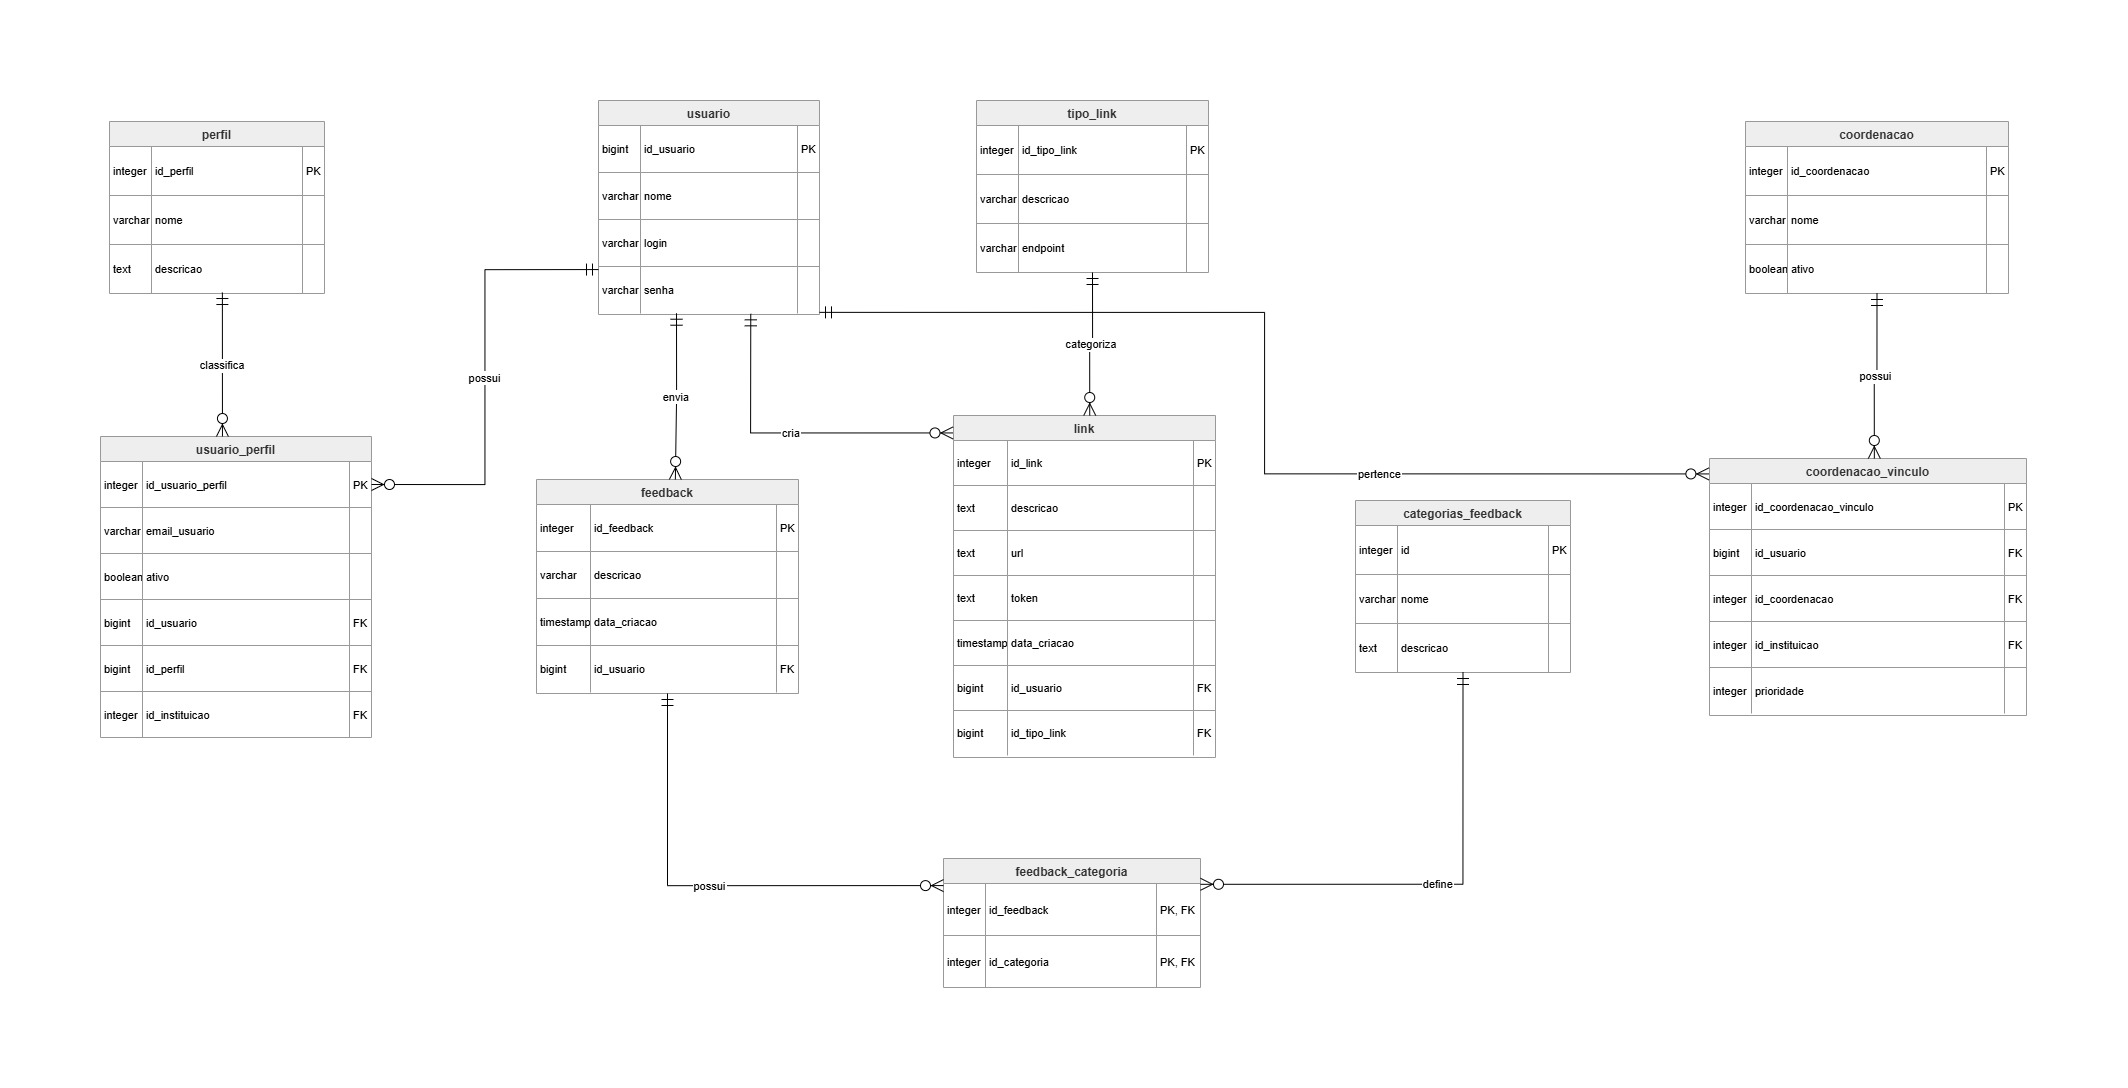
\includegraphics[width=\linewidth,height=0.9\textheight,keepaspectratio]{figuras/Figura_11_Diagrama ER_controle de acesso.jpg}
\fonteautores
\end{figure}

\newpage

\begin{figure}[H]
\centering
\caption{Diagrama de Entidade-Relacionamento: Módulo Acadêmico}
\label{fig:der_academico}
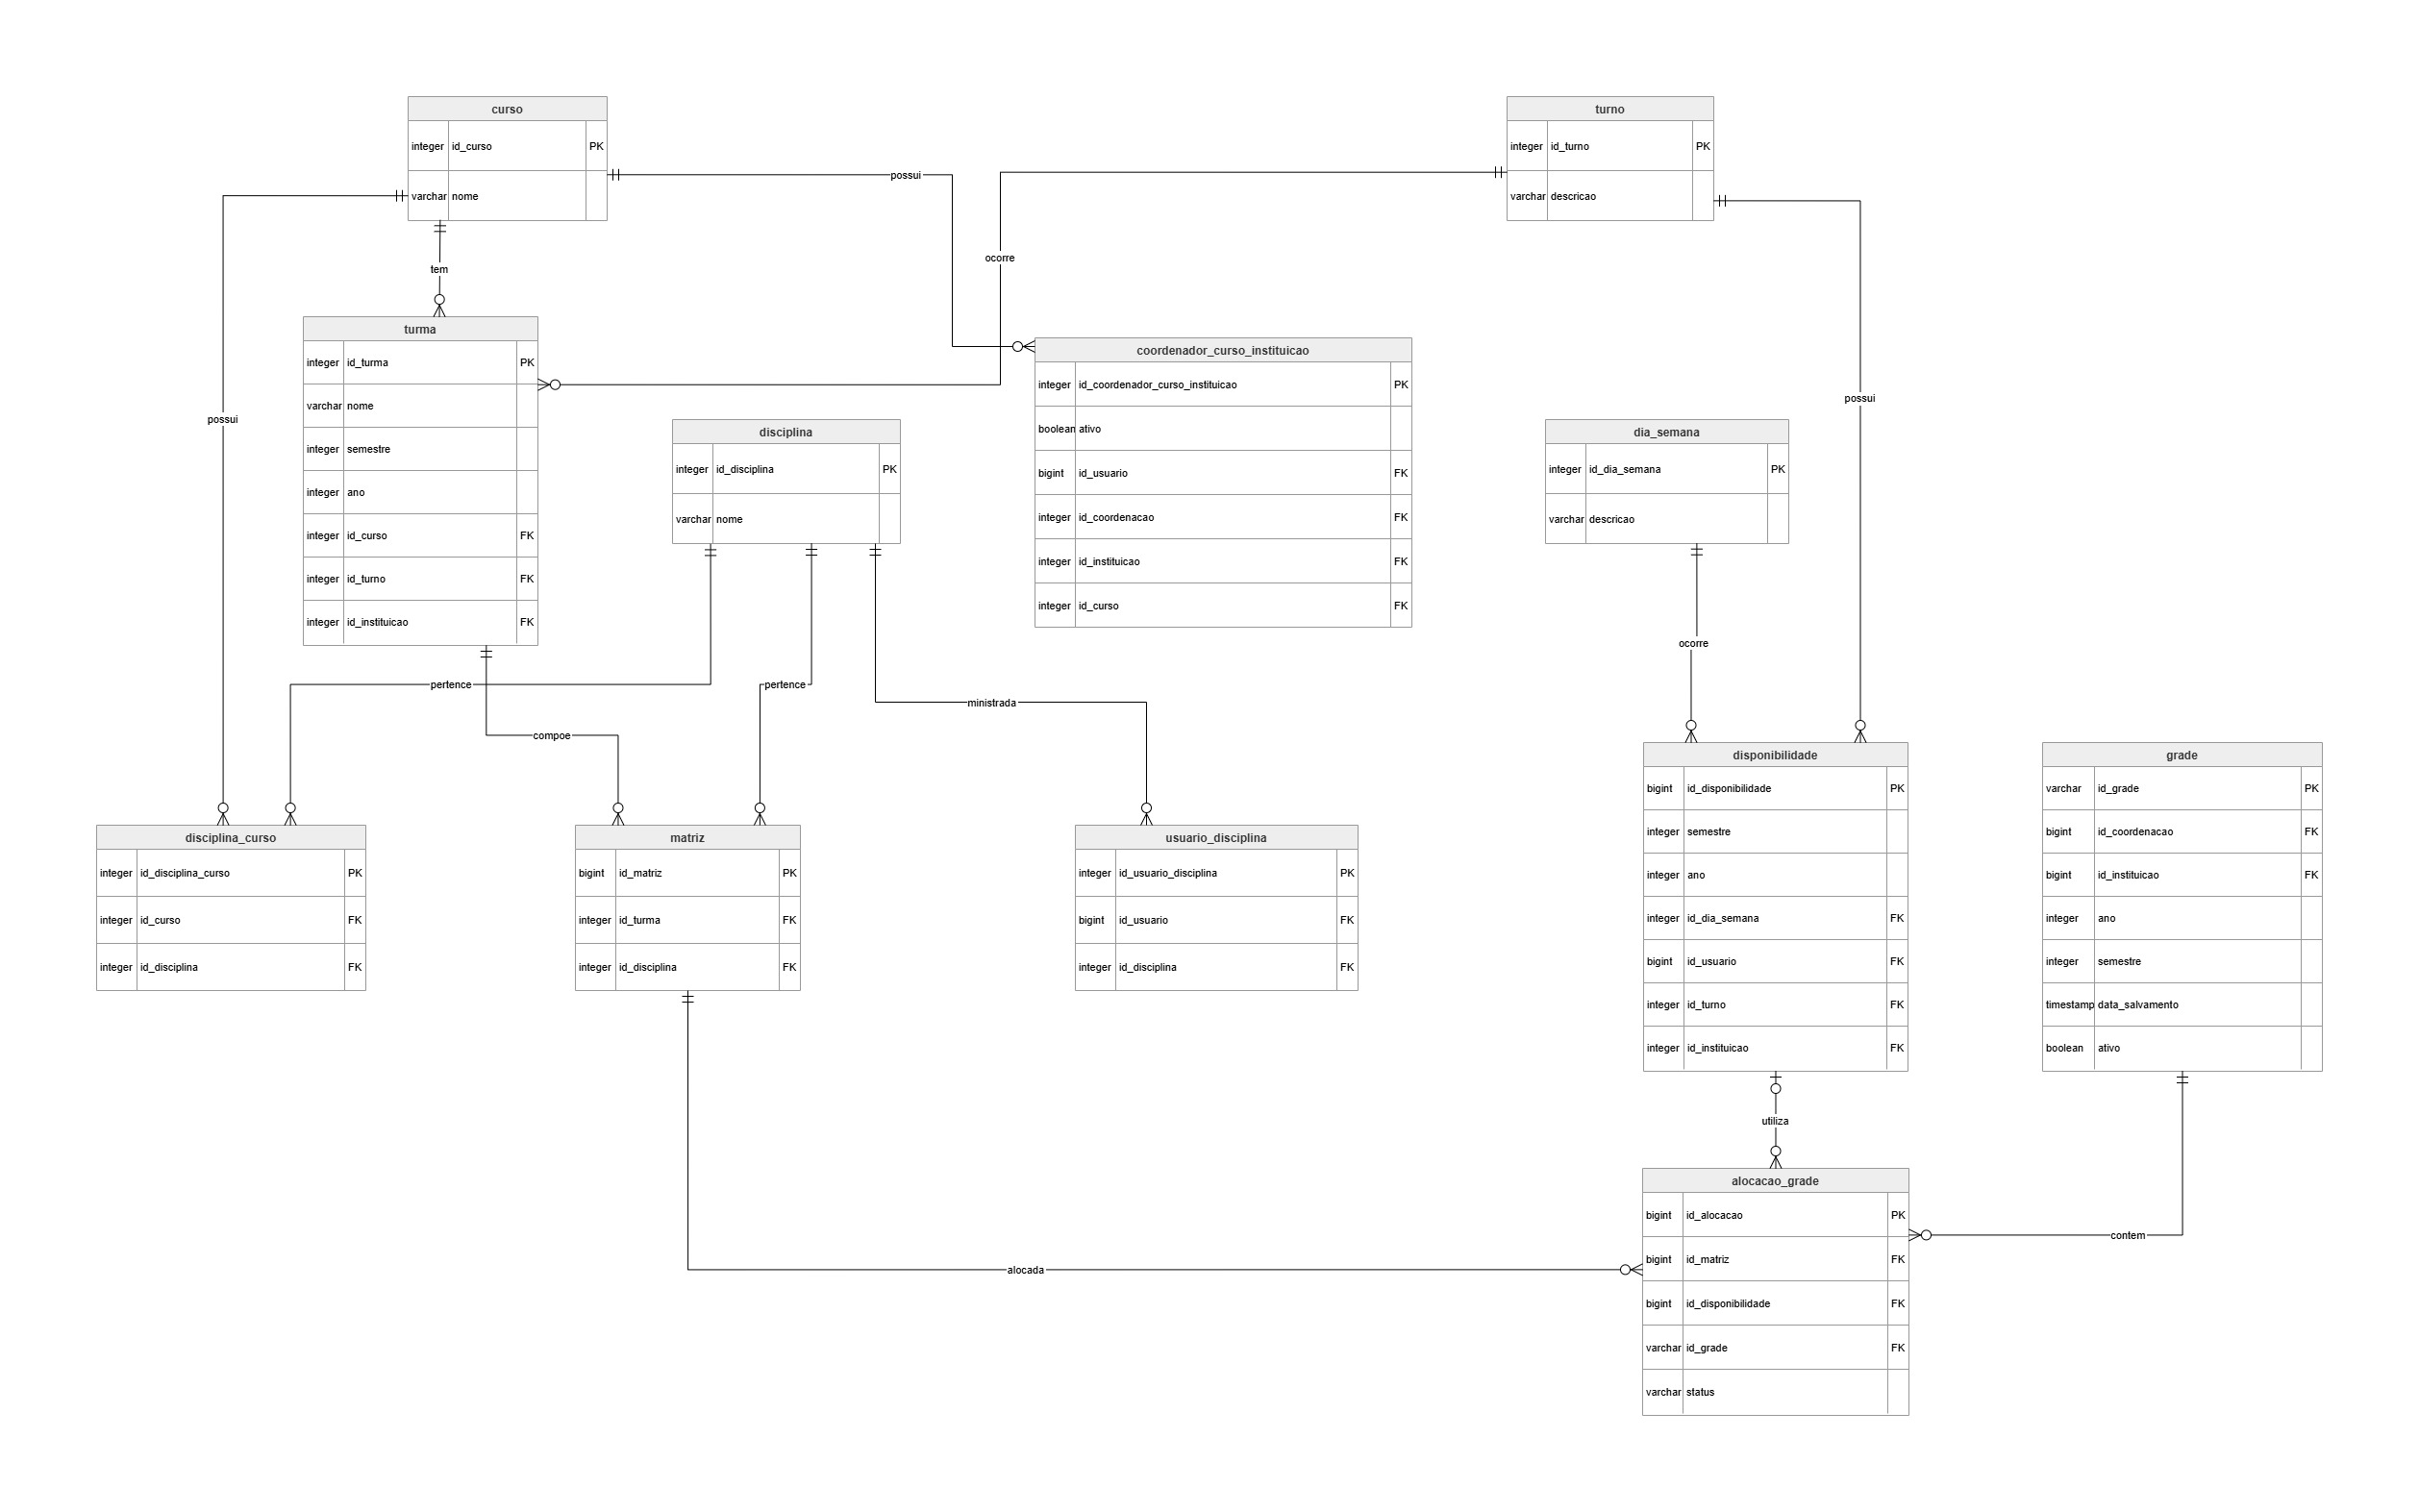
\includegraphics[width=\linewidth,height=0.9\textheight,keepaspectratio]{figuras/Figura_12_diagrama ER_academico.jpg}
\fonteautores
\end{figure}

\newpage

\begin{figure}[H]
\centering
\caption{Diagrama de Entidade-Relacionamento: Módulo Institucional}
\label{fig:der_institucional}
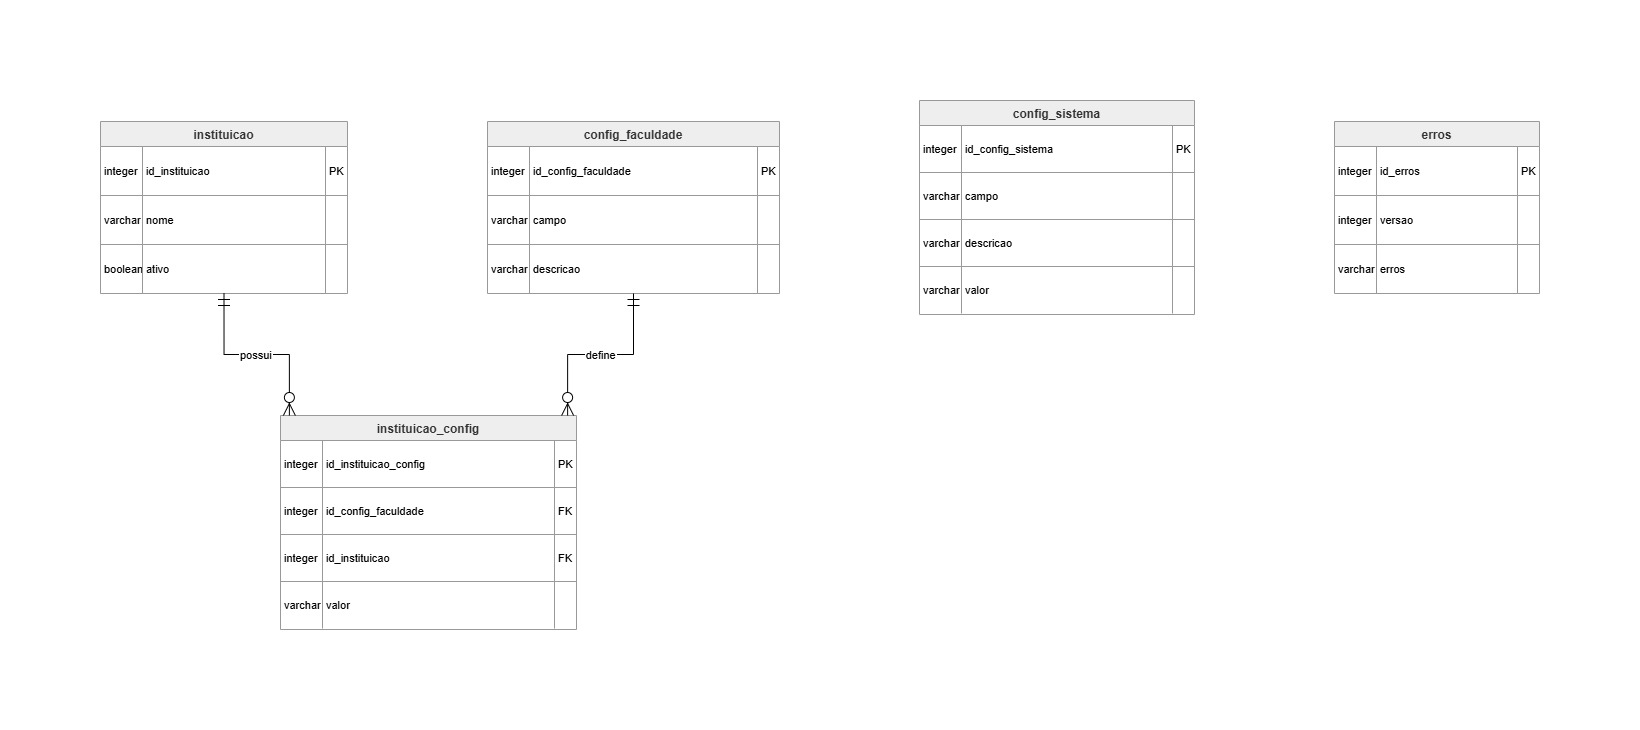
\includegraphics[width=\linewidth,height=0.9\textheight,keepaspectratio]{figuras/Figura_13_diagrama ER instituicao.jpg}
\fonteautores
\end{figure}

\end{landscape}

\begin{landscape}

\begin{figure}[H]
\centering
\caption{Diagrama de Entidade-Relacionamento Completo}
\label{fig:der_completo}
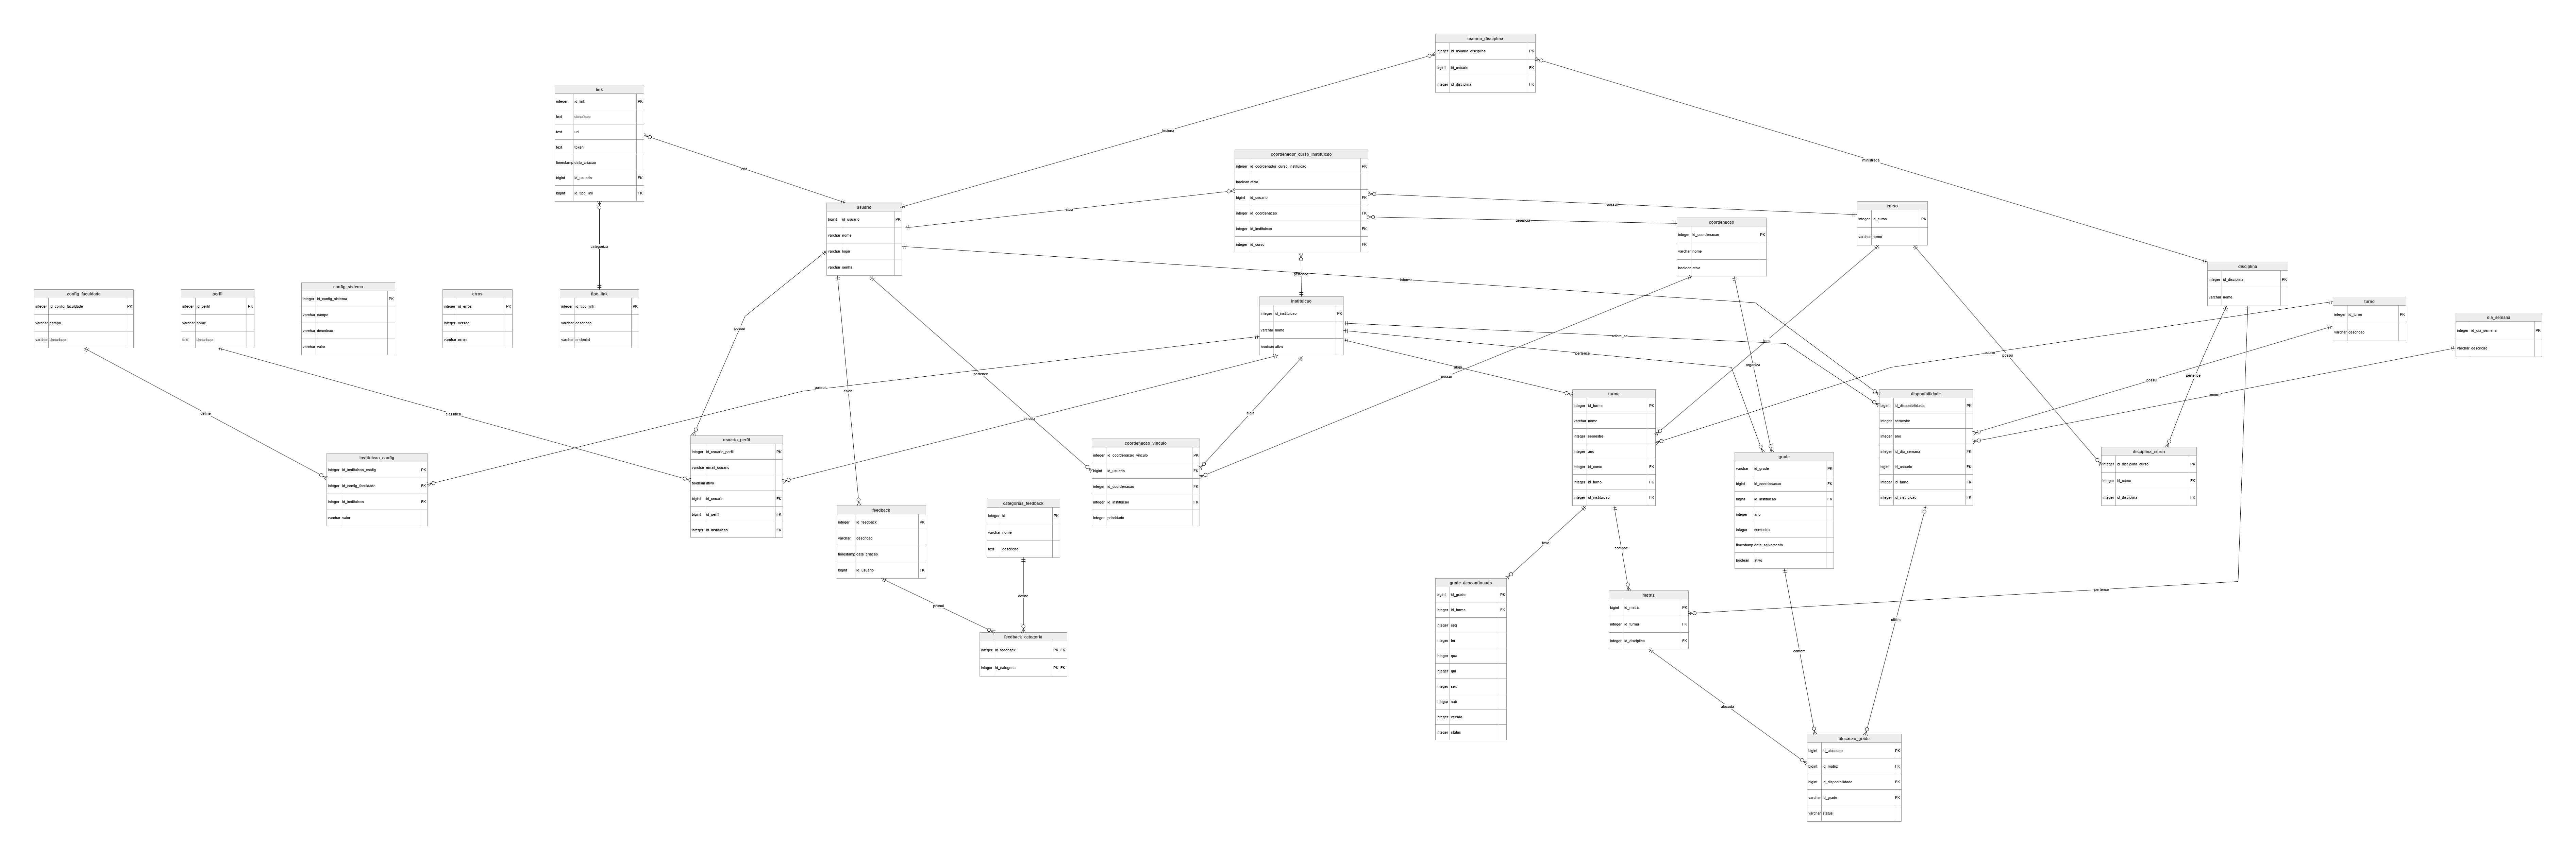
\includegraphics[width=\linewidth,height=\textheight,keepaspectratio]{figuras/Figura_14_diagrama ER completo.jpg}
\fonteautores
\end{figure}

\end{landscape}

\subsection{Dicionário de Dados}
\label{subsec:4.4.2}

\begingroup
\small
\sloppy
\setlength{\tabcolsep}{3pt}

O dicionário de dados complementa a representação gráfica do Modelo Entidade-Relacionamento, descrevendo a estrutura física das tabelas com tipos de dados, restrições de integridade e a semântica de cada atributo. Os Quadros de Tabela 37 a Tabela 63 apresentam a especificação completa das 27 tabelas do banco de dados do IGRIS.

% Tabela 37
\vspace{\baselineskip}

\Needspace{0.32\textheight}
\begin{longtable}{|L{5.2cm}|L{3.2cm}|L{2.4cm}|L{3.4cm}|}
\caption{instituicao} \\
\hline
\textbf{Variável} & \textbf{Tipo} & \textbf{Propriedades} & \textbf{Descrição} \\
\hline
\endfirsthead
\hline
\textbf{Variável} & \textbf{Tipo} & \textbf{Propriedades} & \textbf{Descrição} \\
\hline
\endhead
id\_instituicao & Integer (4 bytes) & PK & Código de identificação da tabela \\
\hline
nome & character varying (255) & NOT NULL & Nome da instituição de ensino \\
\hline
ativo & boolean (1 byte) & NOT NULL & Indica se a instituição está ativa no sistema \\
\hline
\end{longtable}

\fonteautores

% Tabela 38
\vspace{\baselineskip}

\Needspace{0.32\textheight}
\begin{longtable}{|L{5.2cm}|L{3.2cm}|L{2.4cm}|L{3.4cm}|}
\caption{config\_faculdade} \\
\hline
\textbf{Variável} & \textbf{Tipo} & \textbf{Propriedades} & \textbf{Descrição} \\
\hline
\endfirsthead
\hline
\textbf{Variável} & \textbf{Tipo} & \textbf{Propriedades} & \textbf{Descrição} \\
\hline
\endhead
id\_config\_faculdade & Integer (4 bytes) & PK & Código de identificação da tabela \\
\hline
campo & character varying (255) & NOT NULL & Nome identificador da configuração \\
\hline
descricao & character varying (255) & NULL & Descrição textual explicando a finalidade da configuração \\
\hline
\end{longtable}

\fonteautores

% Tabela 39
\vspace{\baselineskip}

\Needspace{0.32\textheight}
\begin{longtable}{|L{5.2cm}|L{3.2cm}|L{2.4cm}|L{3.4cm}|}
\caption{instituicao\_config} \\
\hline
\textbf{Variável} & \textbf{Tipo} & \textbf{Propriedades} & \textbf{Descrição} \\
\hline
\endfirsthead
\hline
\textbf{Variável} & \textbf{Tipo} & \textbf{Propriedades} & \textbf{Descrição} \\
\hline
\endhead
id\_instituicao\_config & Integer (4 bytes) & PK & Código de identificação da tabela \\
\hline
id\_config\_faculdade & Integer (4 bytes) & FK – config\_faculdade & Referência à configuração do catálogo \\
\hline
id\_instituicao & Integer (4 bytes) & FK – instituicao & Referência à instituição dona da configuração \\
\hline
valor & character varying (255) & NULL & Valor atribuído à configuração para esta instituição \\
\hline
\end{longtable}

\fonteautores

% Tabela 40
\vspace{\baselineskip}

\Needspace{0.32\textheight}
\begin{longtable}{|L{5.2cm}|L{3.2cm}|L{2.4cm}|L{3.4cm}|}
\caption{config\_sistema} \\
\hline
\textbf{Variável} & \textbf{Tipo} & \textbf{Propriedades} & \textbf{Descrição} \\
\hline
\endfirsthead
\hline
\textbf{Variável} & \textbf{Tipo} & \textbf{Propriedades} & \textbf{Descrição} \\
\hline
\endhead
id\_config\_sistema & Integer (4 bytes) & PK & Código de identificação da tabela \\
\hline
campo & character varying (255) & NOT NULL & Nome identificador do parâmetro (ex: TAMANHO\_POPULACAO) \\
\hline
descricao & character varying (255) & NULL & Descrição textual explicando o parâmetro \\
\hline
valor & character varying (255) & NULL & Valor atual do parâmetro \\
\hline
\end{longtable}

\fonteautores

% Tabela 41
\vspace{\baselineskip}

\Needspace{0.32\textheight}
\begin{longtable}{|L{5.2cm}|L{3.2cm}|L{2.4cm}|L{3.4cm}|}
\caption{erros} \\
\hline
\textbf{Variável} & \textbf{Tipo} & \textbf{Propriedades} & \textbf{Descrição} \\
\hline
\endfirsthead
\hline
\textbf{Variável} & \textbf{Tipo} & \textbf{Propriedades} & \textbf{Descrição} \\
\hline
\endhead
id\_erros & Integer (4 bytes) & PK & Código de identificação da tabela \\
\hline
versao & Integer (4 bytes) & NULL & Número da versão do sistema no momento do erro \\
\hline
erros & character varying (255) & NULL & Descrição textual do erro registrado \\
\hline
\end{longtable}

\fonteautores

% Tabela 42
\vspace{\baselineskip}

\Needspace{0.32\textheight}
\begin{longtable}{|L{5.2cm}|L{3.2cm}|L{2.4cm}|L{3.4cm}|}
\caption{usuario} \\
\hline
\textbf{Variável} & \textbf{Tipo} & \textbf{Propriedades} & \textbf{Descrição} \\
\hline
\endfirsthead
\hline
\textbf{Variável} & \textbf{Tipo} & \textbf{Propriedades} & \textbf{Descrição} \\
\hline
\endhead
id\_usuario & bigint (8 bytes) & PK & Código de identificação da tabela \\
\hline
nome & character varying (255) & NOT NULL & Nome completo do usuário \\
\hline
login & character varying (255) & NOT NULL, UNIQUE & Login único de acesso ao sistema \\
\hline
senha & character varying (255) & NOT NULL & Senha criptografada (BCrypt) do usuário \\
\hline
\end{longtable}

\fonteautores

% Tabela 43
\vspace{\baselineskip}

\Needspace{0.32\textheight}
\begin{longtable}{|L{5.2cm}|L{3.2cm}|L{2.4cm}|L{3.4cm}|}
\caption{perfil} \\
\hline
\textbf{Variável} & \textbf{Tipo} & \textbf{Propriedades} & \textbf{Descrição} \\
\hline
\endfirsthead
\hline
\textbf{Variável} & \textbf{Tipo} & \textbf{Propriedades} & \textbf{Descrição} \\
\hline
\endhead
id\_perfil & Integer (4 bytes) & PK & Código de identificação da tabela \\
\hline
nome & character varying (255) & NOT NULL & Nome do perfil de acesso \\
\hline
descricao & text (variável) & NULL & Descrição das permissões do perfil \\
\hline
\end{longtable}

\fonteautores

% Tabela 44
\vspace{\baselineskip}

\Needspace{0.32\textheight}
\begin{longtable}{|L{5.2cm}|L{3.2cm}|L{2.4cm}|L{3.4cm}|}
\caption{usuario\_perfil} \\
\hline
\textbf{Variável} & \textbf{Tipo} & \textbf{Propriedades} & \textbf{Descrição} \\
\hline
\endfirsthead
\hline
\textbf{Variável} & \textbf{Tipo} & \textbf{Propriedades} & \textbf{Descrição} \\
\hline
\endhead
id\_usuario\_perfil & Integer (4 bytes) & PK & Código de identificação da tabela \\
\hline
email\_usuario & character varying (255) & NULL & E-mail do usuário neste vínculo específico \\
\hline
ativo & boolean (1 byte) & NOT NULL & Indica se este vínculo de perfil está ativo \\
\hline
id\_usuario & bigint (8 bytes) & FK – usuario & Referência ao usuário \\
\hline
id\_perfil & bigint (8 bytes) & FK – perfil & Referência ao perfil de acesso \\
\hline
id\_instituicao & Integer (4 bytes) & FK – instituicao & Referência à instituição do vínculo \\
\hline
\end{longtable}

\fonteautores

% Tabela 45
\vspace{\baselineskip}

\Needspace{0.32\textheight}
\begin{longtable}{|L{5.2cm}|L{3.2cm}|L{2.4cm}|L{3.4cm}|}
\caption{tipo\_link} \\
\hline
\textbf{Variável} & \textbf{Tipo} & \textbf{Propriedades} & \textbf{Descrição} \\
\hline
\endfirsthead
\hline
\textbf{Variável} & \textbf{Tipo} & \textbf{Propriedades} & \textbf{Descrição} \\
\hline
\endhead
id\_tipo\_link & Integer (4 bytes) & PK & Código de identificação da tabela \\
\hline
descricao & character varying (255) & NOT NULL & Descrição do tipo de link \\
\hline
endpoint & character varying (255) & NULL & Rota/endpoint associado ao tipo de link \\
\hline
\end{longtable}

\fonteautores

% Tabela 46
\vspace{\baselineskip}

\Needspace{0.32\textheight}
\begin{longtable}{|L{5.2cm}|L{3.2cm}|L{2.4cm}|L{3.4cm}|}
\caption{link} \\
\hline
\textbf{Variável} & \textbf{Tipo} & \textbf{Propriedades} & \textbf{Descrição} \\
\hline
\endfirsthead
\hline
\textbf{Variável} & \textbf{Tipo} & \textbf{Propriedades} & \textbf{Descrição} \\
\hline
\endhead
id\_link & Integer (4 bytes) & PK & Código de identificação da tabela \\
\hline
descricao & text (variável) & NULL & Descrição ou finalidade do link gerado \\
\hline
url & text (variável) & NULL & URL completa do link gerado \\
\hline
token & text (variável) & NOT NULL & Token criptografado para validação do link \\
\hline
data\_criacao & timestamp (8 bytes) & NOT NULL & Data e hora da criação do link \\
\hline
id\_usuario & bigint (8 bytes) & FK – usuario & Referência ao usuário que criou o link \\
\hline
id\_tipo\_link & bigint (8 bytes) & FK – tipo\_link & Referência ao tipo de link \\
\hline
\end{longtable}

\fonteautores

% Tabela 47
\vspace{\baselineskip}

\Needspace{0.32\textheight}
\begin{longtable}{|L{5.2cm}|L{3.2cm}|L{2.4cm}|L{3.4cm}|}
\caption{feedback} \\
\hline
\textbf{Variável} & \textbf{Tipo} & \textbf{Propriedades} & \textbf{Descrição} \\
\hline
\endfirsthead
\hline
\textbf{Variável} & \textbf{Tipo} & \textbf{Propriedades} & \textbf{Descrição} \\
\hline
\endhead
id\_feedback & Integer (4 bytes) & PK & Código de identificação da tabela \\
\hline
descricao & character varying (255) & NOT NULL & Texto descritivo do feedback enviado \\
\hline
data\_criacao & timestamp (8 bytes) & NOT NULL & Data e hora do envio do feedback \\
\hline
id\_usuario & bigint (8 bytes) & FK – usuario & Referência ao usuário remetente \\
\hline
\end{longtable}

\fonteautores

% Tabela 48
\vspace{\baselineskip}

\Needspace{0.32\textheight}
\begin{longtable}{|L{5.2cm}|L{3.2cm}|L{2.4cm}|L{3.4cm}|}
\caption{categorias\_feedback} \\
\hline
\textbf{Variável} & \textbf{Tipo} & \textbf{Propriedades} & \textbf{Descrição} \\
\hline
\endfirsthead
\hline
\textbf{Variável} & \textbf{Tipo} & \textbf{Propriedades} & \textbf{Descrição} \\
\hline
\endhead
id & Integer (4 bytes) & PK & Código de identificação da tabela \\
\hline
nome & character varying (255) & NOT NULL & Nome da categoria \\
\hline
descricao & text (variável) & NULL & Descrição detalhada da categoria \\
\hline
\end{longtable}

\fonteautores

% Tabela 49
\vspace{\baselineskip}

\Needspace{0.32\textheight}
\begin{longtable}{|L{5.2cm}|L{3.2cm}|L{2.4cm}|L{3.4cm}|}
\caption{feedback\_categoria} \\
\hline
\textbf{Variável} & \textbf{Tipo} & \textbf{Propriedades} & \textbf{Descrição} \\
\hline
\endfirsthead
\hline
\textbf{Variável} & \textbf{Tipo} & \textbf{Propriedades} & \textbf{Descrição} \\
\hline
\endhead
id\_feedback & Integer (4 bytes) & PK, FK – feedback & Referência ao feedback \\
\hline
id\_categoria & Integer (4 bytes) & PK, FK – categorias\_feedback & Referência à categoria do feedback \\
\hline
\end{longtable}

\fonteautores

% Tabela 50
\vspace{\baselineskip}

\Needspace{0.32\textheight}
\begin{longtable}{|L{5.2cm}|L{3.2cm}|L{2.4cm}|L{3.4cm}|}
\caption{coordenacao} \\
\hline
\textbf{Variável} & \textbf{Tipo} & \textbf{Propriedades} & \textbf{Descrição} \\
\hline
\endfirsthead
\hline
\textbf{Variável} & \textbf{Tipo} & \textbf{Propriedades} & \textbf{Descrição} \\
\hline
\endhead
id\_coordenacao & Integer (4 bytes) & PK & Código de identificação da tabela \\
\hline
nome & character varying (255) & NOT NULL & Nome da coordenação/departamento \\
\hline
ativo & boolean (1 byte) & NOT NULL & Indica se a coordenação está ativa \\
\hline
\end{longtable}

\fonteautores

% Tabela 51
\vspace{\baselineskip}

\Needspace{0.32\textheight}
\begin{longtable}{|L{5.2cm}|L{3.2cm}|L{2.4cm}|L{3.4cm}|}
\caption{coordenacao\_vinculo} \\
\hline
\textbf{Variável} & \textbf{Tipo} & \textbf{Propriedades} & \textbf{Descrição} \\
\hline
\endfirsthead
\hline
\textbf{Variável} & \textbf{Tipo} & \textbf{Propriedades} & \textbf{Descrição} \\
\hline
\endhead
id\_coordenacao\_vinculo & Integer (4 bytes) & PK & Código de identificação da tabela \\
\hline
id\_usuario & bigint (8 bytes) & FK – usuario & Referência ao usuário (coordenador) \\
\hline
id\_coordenacao & Integer (4 bytes) & FK – coordenacao & Referência à coordenação \\
\hline
id\_instituicao & Integer (4 bytes) & FK – instituicao & Referência à instituição \\
\hline
prioridade & Integer (4 bytes) & NULL & Nível de prioridade do vínculo \\
\hline
\end{longtable}

\fonteautores

% Tabela 52
\vspace{\baselineskip}

\Needspace{0.32\textheight}
\begin{longtable}{|L{5.2cm}|L{3.2cm}|L{2.4cm}|L{3.4cm}|}
\caption{curso} \\
\hline
\textbf{Variável} & \textbf{Tipo} & \textbf{Propriedades} & \textbf{Descrição} \\
\hline
\endfirsthead
\hline
\textbf{Variável} & \textbf{Tipo} & \textbf{Propriedades} & \textbf{Descrição} \\
\hline
\endhead
id\_curso & Integer (4 bytes) & PK & Código de identificação da tabela \\
\hline
nome & character varying (255) & NOT NULL & Nome do curso \\
\hline
\end{longtable}

\fonteautores

% Tabela 53
\vspace{\baselineskip}

\Needspace{0.32\textheight}
\begin{longtable}{|L{5.2cm}|L{3.2cm}|L{2.4cm}|L{3.4cm}|}
\caption{turno} \\
\hline
\textbf{Variável} & \textbf{Tipo} & \textbf{Propriedades} & \textbf{Descrição} \\
\hline
\endfirsthead
\hline
\textbf{Variável} & \textbf{Tipo} & \textbf{Propriedades} & \textbf{Descrição} \\
\hline
\endhead
id\_turno & Integer (4 bytes) & PK & Código de identificação da tabela \\
\hline
descricao & character varying (50) & NOT NULL & Nome/descrição do turno \\
\hline
\end{longtable}

\fonteautores

% Tabela 54
\vspace{\baselineskip}

\Needspace{0.32\textheight}
\begin{longtable}{|L{5.2cm}|L{3.2cm}|L{2.4cm}|L{3.4cm}|}
\caption{dia\_semana} \\
\hline
\textbf{Variável} & \textbf{Tipo} & \textbf{Propriedades} & \textbf{Descrição} \\
\hline
\endfirsthead
\hline
\textbf{Variável} & \textbf{Tipo} & \textbf{Propriedades} & \textbf{Descrição} \\
\hline
\endhead
id\_dia\_semana & Integer (4 bytes) & PK & Código de identificação da tabela \\
\hline
descricao & character varying (50) & NOT NULL & Nome do dia da semana \\
\hline
\end{longtable}

\fonteautores

% Tabela 55
\vspace{\baselineskip}

\Needspace{0.32\textheight}
\begin{longtable}{|L{5.2cm}|L{3.2cm}|L{2.4cm}|L{3.4cm}|}
\caption{disciplina} \\
\hline
\textbf{Variável} & \textbf{Tipo} & \textbf{Propriedades} & \textbf{Descrição} \\
\hline
\endfirsthead
\hline
\textbf{Variável} & \textbf{Tipo} & \textbf{Propriedades} & \textbf{Descrição} \\
\hline
\endhead
id\_disciplina & Integer (4 bytes) & PK & Código de identificação da tabela \\
\hline
nome & character varying (255) & NOT NULL & Nome da disciplina \\
\hline
\end{longtable}

\fonteautores

% Tabela 56
\vspace{\baselineskip}

\Needspace{0.32\textheight}
\begin{longtable}{|L{5.2cm}|L{3.2cm}|L{2.4cm}|L{3.4cm}|}
\caption{turma} \\
\hline
\textbf{Variável} & \textbf{Tipo} & \textbf{Propriedades} & \textbf{Descrição} \\
\hline
\endfirsthead
\hline
\textbf{Variável} & \textbf{Tipo} & \textbf{Propriedades} & \textbf{Descrição} \\
\hline
\endhead
id\_turma & Integer (4 bytes) & PK & Código de identificação da tabela \\
\hline
nome & character varying (255) & NOT NULL & Nome ou identificador da turma \\
\hline
semestre & Integer (4 bytes) & NOT NULL & Semestre letivo da turma (1 ou 2) \\
\hline
ano & Integer (4 bytes) & NOT NULL & Ano letivo da turma \\
\hline
id\_curso & Integer (4 bytes) & FK – curso & Referência ao curso da turma \\
\hline
id\_turno & Integer (4 bytes) & FK – turno & Referência ao turno da turma \\
\hline
id\_instituicao & Integer (4 bytes) & FK – instituicao & Referência à instituição da turma \\
\hline
\end{longtable}

\fonteautores

% Tabela 57
\vspace{\baselineskip}

\Needspace{0.32\textheight}
\begin{longtable}{|L{5.2cm}|L{3.2cm}|L{2.4cm}|L{3.4cm}|}
\caption{disciplina\_curso} \\
\hline
\textbf{Variável} & \textbf{Tipo} & \textbf{Propriedades} & \textbf{Descrição} \\
\hline
\endfirsthead
\hline
\textbf{Variável} & \textbf{Tipo} & \textbf{Propriedades} & \textbf{Descrição} \\
\hline
\endhead
id\_disciplina\_curso & Integer (4 bytes) & PK & Código de identificação da tabela \\
\hline
id\_curso & Integer (4 bytes) & FK – curso & Referência ao curso \\
\hline
id\_disciplina & Integer (4 bytes) & FK – disciplina & Referência à disciplina \\
\hline
\end{longtable}

\fonteautores

% Tabela 58
\vspace{\baselineskip}

\Needspace{0.32\textheight}
\begin{longtable}{|L{5.2cm}|L{3.2cm}|L{2.4cm}|L{3.4cm}|}
\caption{matriz} \\
\hline
\textbf{Variável} & \textbf{Tipo} & \textbf{Propriedades} & \textbf{Descrição} \\
\hline
\endfirsthead
\hline
\textbf{Variável} & \textbf{Tipo} & \textbf{Propriedades} & \textbf{Descrição} \\
\hline
\endhead
id\_matriz & bigint (8 bytes) & PK & Código de identificação da tabela \\
\hline
id\_turma & Integer (4 bytes) & FK – turma & Referência à turma \\
\hline
id\_disciplina & Integer (4 bytes) & FK – disciplina & Referência à disciplina \\
\hline
\end{longtable}

\fonteautores

% Tabela 59
\vspace{\baselineskip}

\Needspace{0.32\textheight}
\begin{longtable}{|L{5.2cm}|L{3.2cm}|L{2.4cm}|L{3.4cm}|}
\caption{coordenador\_curso\_instituicao} \\
\hline
\textbf{Variável} & \textbf{Tipo} & \textbf{Propriedades} & \textbf{Descrição} \\
\hline
\endfirsthead
\hline
\textbf{Variável} & \textbf{Tipo} & \textbf{Propriedades} & \textbf{Descrição} \\
\hline
\endhead
id\_coordenador\_curso\_instituicao & Integer (4 bytes) & PK & Código de identificação da tabela \\
\hline
ativo & boolean (1 byte) & NOT NULL & Indica se o vínculo está ativo \\
\hline
id\_usuario & bigint (8 bytes) & FK – usuario & Referência ao usuário (coordenador) \\
\hline
id\_coordenacao & Integer (4 bytes) & FK – coordenacao & Referência à coordenação \\
\hline
id\_instituicao & Integer (4 bytes) & FK – instituicao & Referência à instituição \\
\hline
id\_curso & Integer (4 bytes) & FK – curso & Referência ao curso gerenciado \\
\hline
\end{longtable}

\fonteautores

% Tabela 60
\vspace{\baselineskip}

\Needspace{0.32\textheight}
\begin{longtable}{|L{5.2cm}|L{3.2cm}|L{2.4cm}|L{3.4cm}|}
\caption{usuario\_disciplina} \\
\hline
\textbf{Variável} & \textbf{Tipo} & \textbf{Propriedades} & \textbf{Descrição} \\
\hline
\endfirsthead
\hline
\textbf{Variável} & \textbf{Tipo} & \textbf{Propriedades} & \textbf{Descrição} \\
\hline
\endhead
id\_usuario\_disciplina & Integer (4 bytes) & PK & Código de identificação da tabela \\
\hline
id\_usuario & bigint (8 bytes) & FK – usuario & Referência ao usuário (professor) \\
\hline
id\_disciplina & Integer (4 bytes) & FK – disciplina & Referência à disciplina \\
\hline
\end{longtable}

\fonteautores

% Tabela 61
\vspace{\baselineskip}

\Needspace{0.32\textheight}
\begin{longtable}{|L{5.2cm}|L{3.2cm}|L{2.4cm}|L{3.4cm}|}
\caption{disponibilidade} \\
\hline
\textbf{Variável} & \textbf{Tipo} & \textbf{Propriedades} & \textbf{Descrição} \\
\hline
\endfirsthead
\hline
\textbf{Variável} & \textbf{Tipo} & \textbf{Propriedades} & \textbf{Descrição} \\
\hline
\endhead
id\_disponibilidade & bigint (8 bytes) & PK & Código de identificação da tabela \\
\hline
semestre & Integer (4 bytes) & NOT NULL & Semestre de referência da disponibilidade \\
\hline
ano & Integer (4 bytes) & NOT NULL & Ano de referência da disponibilidade \\
\hline
id\_dia\_semana & Integer (4 bytes) & FK – dia\_semana & Referência ao dia da semana disponível \\
\hline
id\_usuario & bigint (8 bytes) & FK – usuario & Referência ao usuário (professor) \\
\hline
id\_turno & Integer (4 bytes) & FK – turno & Referência ao turno disponível \\
\hline
id\_instituicao & Integer (4 bytes) & FK – instituicao & Referência à instituição do vínculo \\
\hline
\end{longtable}

\fonteautores

% Tabela 62
\vspace{\baselineskip}

\Needspace{0.32\textheight}
\begin{longtable}{|L{5.2cm}|L{3.2cm}|L{2.4cm}|L{3.4cm}|}
\caption{grade} \\
\hline
\textbf{Variável} & \textbf{Tipo} & \textbf{Propriedades} & \textbf{Descrição} \\
\hline
\endfirsthead
\hline
\textbf{Variável} & \textbf{Tipo} & \textbf{Propriedades} & \textbf{Descrição} \\
\hline
\endhead
id\_grade & character varying (36) & PK (UUID) & Código de identificação da tabela \\
\hline
id\_coordenacao & bigint (8 bytes) & FK – coordenacao & Referência à coordenação dona da grade \\
\hline
id\_instituicao & bigint (8 bytes) & FK – instituicao & Referência à instituição \\
\hline
ano & Integer (4 bytes) & NOT NULL & Ano letivo da grade \\
\hline
semestre & Integer (4 bytes) & NOT NULL & Semestre letivo da grade \\
\hline
data\_salvamento & timestamp (8 bytes) & NULL & Data e hora em que a grade foi salva \\
\hline
ativo & boolean (1 byte) & NOT NULL & Indica se a grade está ativa (em vigor) \\
\hline
\end{longtable}

\fonteautores

% Tabela 63
\vspace{\baselineskip}

\Needspace{0.32\textheight}
\begin{longtable}{|L{5.2cm}|L{3.2cm}|L{2.4cm}|L{3.4cm}|}
\caption{alocacao\_grade} \\
\hline
\textbf{Variável} & \textbf{Tipo} & \textbf{Propriedades} & \textbf{Descrição} \\
\hline
\endfirsthead
\hline
\textbf{Variável} & \textbf{Tipo} & \textbf{Propriedades} & \textbf{Descrição} \\
\hline
\endhead
id\_alocacao & bigint (8 bytes) & PK & Código de identificação da tabela \\
\hline
id\_matriz & bigint (8 bytes) & FK – matriz & Referência à matriz (turma + disciplina) \\
\hline
id\_disponibilidade & bigint (8 bytes) & FK – disponibilidade & Referência à disponibilidade (professor + dia + turno) \\
\hline
id\_grade & character varying (36) & FK – grade & Referência à grade à qual esta alocação pertence \\
\hline
status & character varying (50) & NULL & Status da alocação (ex: confirmada, pendente) \\
\hline
\end{longtable}

\fonteautores

\endgroup

% Chapter 6



\chapter{Implementação do Algoritmo Genético}
\label{cap:implementacao}

A implementação dos algoritmos genéticos no sistema IGRIS representa a aplicação prática dos conceitos apresentados nos capítulos anteriores. Enquanto a fundamentação teórica discutiu os princípios dos Algoritmos Genéticos e sua utilização em problemas de busca e otimização, este capítulo apresenta como esses conceitos foram empregados, de maneira concreta, na geração automatizada de grades horárias acadêmicas.

O problema tratado pelo sistema está inserido no contexto do \textit{University Course Timetabling Problem} (UCTP), que envolve a distribuição de demandas acadêmicas em horários disponíveis, considerando restrições como turma, turno, professor habilitado, disponibilidade docente e conflitos de alocação \cite{premananda2024}. Trata-se de um problema combinatório, pois o número de combinações possíveis cresce significativamente conforme aumentam a quantidade de turmas, disciplinas, professores e horários, característica recorrente em problemas de timetabling educacional \cite{ceschia2023}. Diante desse cenário, uma busca exaustiva torna-se pouco viável, o que justifica o uso de métodos aproximativos e meta-heurísticos, como os Algoritmos Genéticos \cite{eiben2015}.

No IGRIS, essa abordagem foi implementada por meio de diferentes serviços de otimização, denominados Sunny, Morpheus e Rocket, responsáveis pela geração automatizada de grades horárias a partir dos dados acadêmicos enviados pelo núcleo do sistema. Embora todos compartilhem o mesmo objetivo de construir, avaliar e retornar a melhor grade encontrada com base em uma função \textit{fitness} e em operadores evolutivos, cada serviço organiza internamente esse processo de maneira distinta, com diferenças na representação dos dados, na formação da população inicial, na avaliação das soluções e no tratamento de conflitos.

Como discutido anteriormente, Algoritmos Genéticos não têm como finalidade garantir, necessariamente, a obtenção da solução ótima global. Seu objetivo é encontrar soluções satisfatórias dentro de um tempo computacional aceitável, especialmente em espaços de busca extensos e complexos \cite{goldberg1989}. Essa característica está presente nos algoritmos do IGRIS, que trabalham com sucessivas gerações de grades candidatas, avaliando sua qualidade, preservando boas soluções e explorando novas combinações por meio de seleção, recombinação e mutação. Assim, a resposta final corresponde à melhor grade identificada durante a execução, considerando as restrições acadêmicas e os parâmetros configurados no sistema.
\section{Implementação do Algoritmo Sunny}
\label{sec:7.1}

No Sunny, a execução do algoritmo genético ocorre no serviço responsável pela geração da grade horária. Esse serviço recebe uma requisição contendo os dados acadêmicos necessários ao processo de alocação, como turmas, matrizes curriculares, disponibilidades docentes e vínculos entre usuários e disciplinas. A partir dessas informações, o algoritmo constrói uma estrutura de contexto denominada EvolutionContext, utilizada para organizar os parâmetros, os mapas auxiliares e os caches necessários durante uma execução específica.

Essa organização é importante porque o algoritmo genético realiza avaliações repetidas. A cada geração, vários indivíduos são avaliados, selecionados, recombinados e modificados. Caso todas essas verificações fossem feitas diretamente sobre as listas originais da requisição, o custo computacional tenderia a ser maior e a implementação ficaria menos eficiente. Por esse motivo, o Sunny cria estruturas de acesso rápido, como mapas de disponibilidades, matrizes, turmas, professores habilitados por disciplina, disponibilidades por turno, turno obrigatório de cada matriz, usuário associado a cada disponibilidade e dia da semana correspondente a cada horário.

Essa etapa pode ser compreendida como uma adaptação prática do conceito de ambiente apresentado no Capítulo 3. Na biologia, o ambiente é o espaço em que os organismos competem, sobrevivem e são selecionados. No algoritmo genético, esse ambiente é representado pelo próprio problema e por suas restrições. No caso do Sunny, ele é formado pelas regras de alocação acadêmica: uma matriz curricular precisa ser associada a uma disponibilidade compatível, o professor precisa estar habilitado para a disciplina, o turno da disponibilidade deve corresponder ao turno da turma e conflitos de horário precisam ser evitados.

A implementação estabelece que os valores utilizados pelo microsserviço sejam definidos por meio de parâmetros armazenados na tabela de configuração do sistema principal, permitindo ao administrador personalizar o comportamento do algoritmo conforme as necessidades institucionais. Atualmente, o banco de dados possui valores padrão definidos a partir de um extenso processo de testes de desempenho, os quais serão detalhados em seção específica, em que diferentes configurações foram avaliadas com o objetivo de identificar aquelas que apresentavam melhor performance, menor incidência de erros, menor tempo de execução e menor consumo de recursos durante a geração das grades.

A forma como uma solução é representada é uma das decisões mais relevantes em um algoritmo genético. No Sunny, cada gene é composto por dois elementos principais: matrizId e disponibilidadeId. O campo matrizId identifica a demanda acadêmica que precisa ser alocada, enquanto o campo disponibilidadeId indica a disponibilidade escolhida para essa demanda. O cromossomo, por sua vez, é formado por uma lista desses genes e representa uma grade horária candidata completa. Essa codificação traduz o problema real para uma estrutura que pode ser manipulada computacionalmente. No domínio acadêmico, o sistema precisa montar uma grade de aulas. No domínio genético, o algoritmo trabalha com listas de pares entre matrizes e disponibilidades. Quando uma demanda não pode ser alocada de maneira compatível, o Sunny utiliza o valor ID\_NAO\_ALOCADO = 0.

A população inicial do Sunny é formada por cromossomos gerados a partir dos dados recebidos na requisição. Essa geração não ocorre de forma totalmente aleatória. Para cada matriz curricular, o Sunny verifica inicialmente o turno obrigatório associado à turma, busca as disponibilidades compatíveis com esse turno, identifica os professores habilitados para a disciplina correspondente e filtra as disponibilidades pertencentes a esses professores. Somente após essa etapa de filtragem o algoritmo escolhe aleatoriamente uma disponibilidade entre as alternativas consideradas válidas. Essa abordagem pode ser classificada como uma inicialização aleatória guiada por restrições, aproximando-se da ideia de codificação restritiva discutida por \citeonline{michalewicz1996}.

A função \textit{fitness} é o mecanismo utilizado pelo Sunny para medir a qualidade de cada cromossomo. No Sunny, a avaliação começa com uma pontuação base proporcional ao número de genes do cromossomo, com valor padrão de 10 pontos por gene. Em seguida, a função percorre os genes e aplica penalidades ou bônus conforme as condições encontradas. Quando um gene está marcado como não alocado, o indivíduo recebe uma penalidade padrão de 10.000 pontos. A mesma penalidade de 10.000 pontos é aplicada quando os dados necessários à avaliação estão incompletos ou inválidos, como ausência de professor, dia ou turno associado à alocação. O Sunny também verifica conflitos de professor por meio de uma chave composta por usuário, dia e turno. Se mais de uma matriz for associada ao mesmo professor no mesmo período, o algoritmo identifica uma colisão e aplica 10.000 pontos de penalidade para cada conflito excedente. A função \textit{fitness} também aplica um bônus de diversidade associado à quantidade de matrizes atribuídas a um professor, com valor padrão de 5 pontos para cada matriz adicional, de modo que ele atua como critério secundário sem se sobrepor à prioridade de reduzir alocações inválidas.

Após a avaliação, o Sunny ordena os indivíduos e aplica duas estratégias: elitismo e seleção por torneio. O elitismo preserva diretamente uma parcela dos melhores indivíduos para a geração seguinte, evitando que boas soluções sejam perdidas por alterações dos operadores evolutivos. A seleção dos pais é realizada por torneio, no qual o algoritmo escolhe aleatoriamente um grupo de indivíduos e seleciona o melhor entre eles, criando pressão seletiva com grau de aleatoriedade que preserva a diversidade populacional.

O \textit{crossover} do Sunny utiliza uma estratégia próxima do \textit{crossover} uniforme, em que o método percorre cada posição do cromossomo e decide aleatoriamente se o gene daquela posição será herdado do primeiro ou do segundo pai. A mutação é aplicada gene a gene: para cada gene, o algoritmo sorteia uma probabilidade e, caso seja inferior à taxa configurada, substitui a disponibilidade associada àquela matriz. Quando a mutação ocorre, o Sunny não escolhe uma nova disponibilidade de forma irrestrita; o algoritmo consulta novamente o turno obrigatório e filtra os professores habilitados antes de escolher aleatoriamente uma alternativa válida.

Após a recombinação e a mutação, o Sunny executa um mecanismo de reparo parcial que identifica situações em que uma mesma turma possui mais de uma alocação no mesmo dia e turno. Quando isso ocorre, o algoritmo preserva a primeira ocorrência e marca as demais como não alocadas. O Sunny não realiza reparo por realocação; o que existe é um reparo parcial por invalidação de alocações conflitantes. Essa abordagem combina duas estratégias de tratamento de restrições: reparo e penalização.

Ao final da execução, o melhor cromossomo encontrado é decodificado em uma lista de alocações de grade. Na decodificação, cada gene é transformado em uma estrutura de alocação contendo turma, matriz, disciplina, disponibilidade, professor e status. O Sunny calcula então as métricas finais, que contabilizam disciplinas não alocadas, inconsistências de turno e conflitos de horário de professor. O ciclo evolutivo é executado até atingir o número máximo de gerações definido nos parâmetros, registrando ao longo da execução a geração em que uma solução sem erros é encontrada, sem que isso interrompa o laço evolutivo.


\begin{figure}[H]
\centering
\caption{Fluxo de execução do algoritmo genético Sunny}
\label{fig:fluxo-sunny}

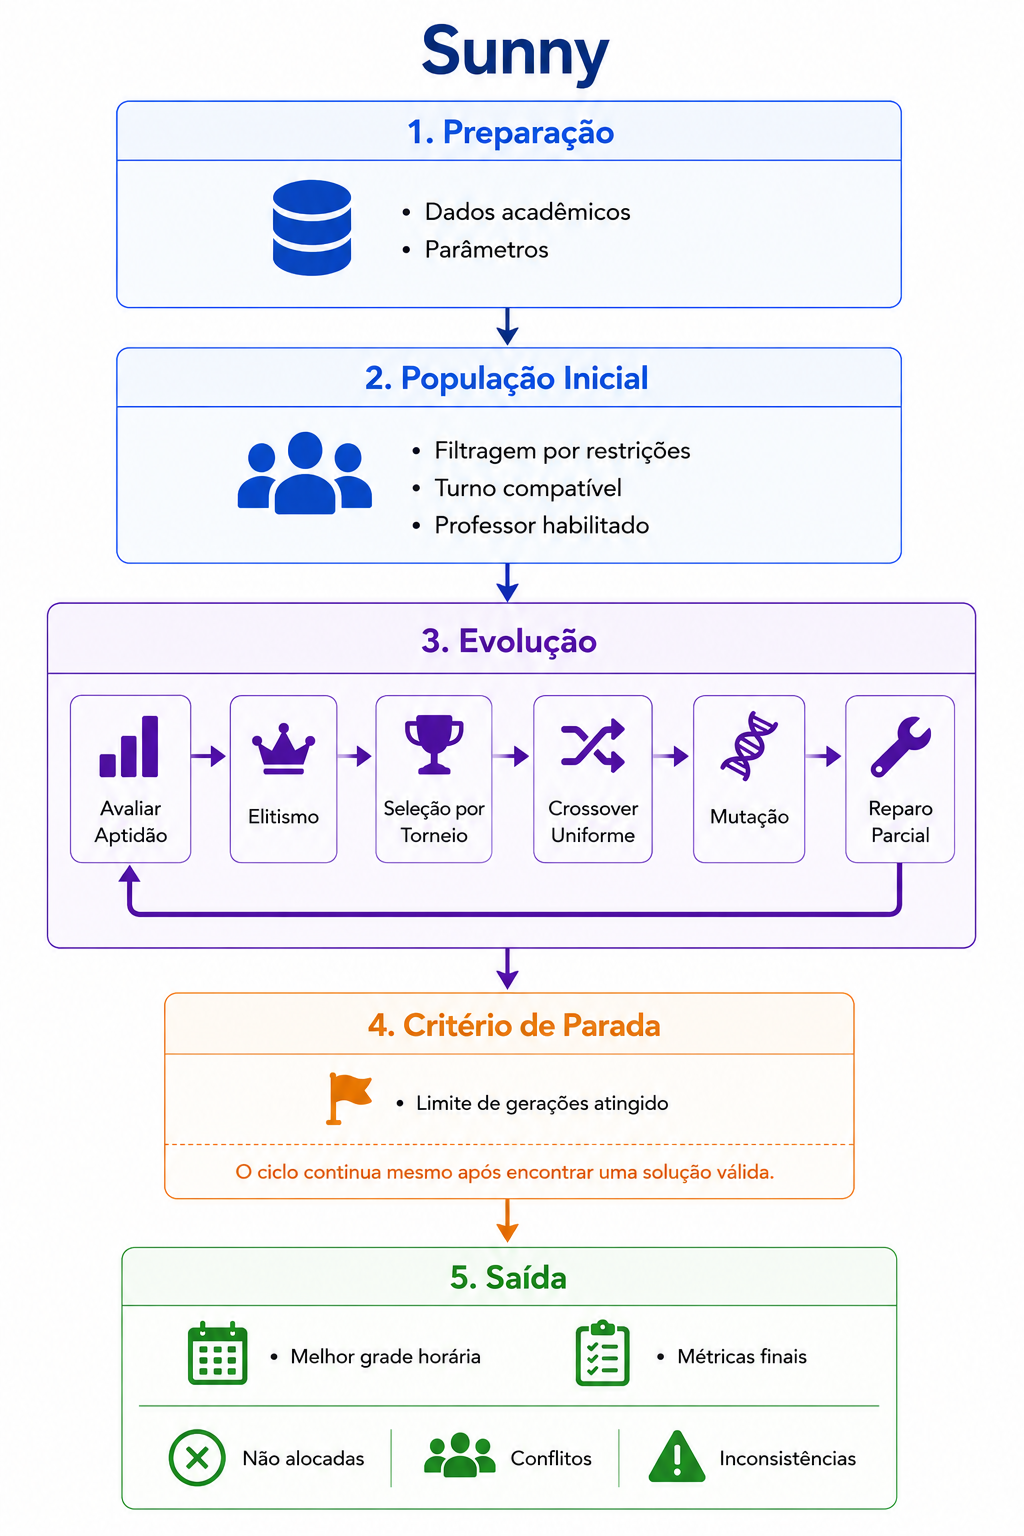
\includegraphics[width=0.85\textwidth]{figuras/Figura_15_ilustracaoFluxoSunny.png}

\vspace{0.2cm}
\fonteautores
\end{figure}

\section{Implementação do Algoritmo Morpheus}
\label{sec:7.2}

No Morpheus, a execução do algoritmo genético ocorre principalmente na classe GradeService, responsável por receber os dados acadêmicos, organizar as estruturas internas de processamento, gerar a população inicial, aplicar os operadores evolutivos e retornar a melhor grade horária encontrada. A entrada principal do algoritmo é uma requisição do tipo GradeRequest, composta por disponibilidades docentes, matrizes curriculares, turmas, vínculos entre professores e disciplinas, parâmetros do algoritmo genético e parâmetros da função \textit{fitness}.

A obtenção dos dados pode ocorrer por meio de uma camada externa ao algoritmo, responsável por consultar o banco de dados e montar a estrutura de entrada. No arquivo data\_service.py, são buscadas disponibilidades, matrizes, turmas e vínculos entre usuários e disciplinas. Entretanto, a execução do algoritmo genético em si não realiza consultas diretas ao banco: o GradeService recebe uma requisição já estruturada, constrói seus índices e caches em memória e, a partir dessas informações, executa o processo evolutivo.

Antes de iniciar a evolução, o Morpheus constrói índices em memória por meio do método \_construir\_indices. Essa etapa transforma as listas recebidas na requisição em estruturas de acesso rápido, criando mapas para recuperar disponibilidades, matrizes e turmas por seus identificadores, além de caches que relacionam disciplinas aos professores habilitados, turnos às disponibilidades e associações entre matrizes, turmas e turnos. Entre essas estruturas, destaca-se o cache de candidatos por matriz: para cada matriz curricular, o algoritmo identifica quais disponibilidades podem ser utilizadas, considerando o turno da turma e o vínculo entre professor e disciplina.

A representação genética do Morpheus utiliza explicitamente uma dataclass chamada Gene, com dois campos: matriz\_id e disponibilidade\_id. O cromossomo, formado por uma lista de genes, corresponde a uma grade horária candidata completa. Além da classe Gene, o Morpheus define a dataclass Individuo, que armazena o cromossomo e sua respectiva \textit{fitness}, e a dataclass Metricas, que concentra informações como quantidade de erros, conflitos, disciplinas não alocadas e dados inválidos. Quando uma matriz não possui candidatos válidos, o Morpheus utiliza o valor ID\_NAO\_ALOCADO = 0.

A população inicial é gerada pelo método \_inicializar\_populacao, que cria cromossomos por meio do método \_gerar\_cromossomo. Para cada matriz, o algoritmo verifica se existem turno, disciplina e turma associados e consulta a lista de candidatos válidos previamente construída. Caso existam candidatos, o algoritmo escolhe aleatoriamente uma disponibilidade, tentando priorizar aquelas que ainda não geram colisão para a mesma turma no mesmo dia e turno. Essa estratégia pode ser classificada como uma inicialização aleatória guiada por restrições.

A função \textit{fitness} é implementada no método \_calcular\_fitness. A avaliação começa com uma pontuação base proporcional ao tamanho do cromossomo, acrescida de bônus por alocações válidas e bônus de diversidade. As penalidades são os elementos mais decisivos: genes não alocados recebem penalidade padrão de 10.000 pontos; conflitos de professor recebem 12.000 pontos, por serem considerados os mais críticos; conflitos de turma recebem 8.000 pontos; dados inválidos recebem 10.000 pontos. Essa hierarquia de pesos demonstra uma priorização interna da implementação.

A evolução da população ocorre por meio do método \_evoluir\_populacao, que combina elitismo, seleção por torneio com \textit{crossover} de um ponto, mutação gene a gene, melhoria local e reparo inteligente. O \textit{crossover} de um ponto sorteia uma posição de corte no cromossomo, de modo que o primeiro filho recebe os genes iniciais do primeiro pai e os genes finais do segundo. A mutação é guiada por restrições do domínio, selecionando a nova disponibilidade dentro do conjunto de candidatos válidos da matriz correspondente.

Uma característica própria do Morpheus é a existência de uma etapa explícita de melhoria local antes do reparo inteligente. Após a mutação, o método \_melhorar\_alocacoes\_locais percorre o cromossomo buscando genes não alocados e tenta encontrar um candidato capaz de preencher a lacuna com pontuação interna de conflito igual a zero. Em seguida, o método \_reparar\_inteligente percorre o cromossomo em até duas passagens, identificando genes problemáticos e buscando o melhor candidato dentro das disponibilidades válidas por meio de uma pontuação interna de conflito. Quando encontra uma opção sem conflito, realiza a substituição; quando não há solução perfeita, pode aceitar uma melhoria parcial.

O critério de parada do Morpheus combina um limite fixo de gerações com mecanismos de parada antecipada. A execução pode ser interrompida quando uma solução sem erros é encontrada, isto é, quando a melhor grade da geração possui quantidade total de erros igual a zero. Na implementação, esse total corresponde à soma entre disciplinas não alocadas, conflitos de professor, conflitos de turma e dados inválidos ou incompletos. Quando essa condição ocorre, a geração da solução sem erros é registrada e o processo evolutivo é encerrado imediatamente.

Além disso, o Morpheus interrompe a evolução quando passa muitas gerações sem melhorar a melhor \textit{fitness} global. O limite de gerações sem melhoria é calculado como 20\% do total de gerações configurado, respeitando um mínimo de 25 e um máximo de 200 gerações, conforme a expressão \texttt{max(25, min(200, numeroGeracoes * 0.20))}. Assim, para 100 gerações configuradas, o limite sem melhoria é 25; para 1.000 gerações, é 200; e para 2.000 gerações, permanece em 200. A melhora considerada nesse critério é uma melhora de \textit{fitness}, não apenas uma redução direta da quantidade de erros. Caso a diferença entre a geração atual e a última geração com melhora alcance esse limite, a execução é interrompida e a resposta indica parada antecipada.

Por fim, se nenhuma das condições anteriores for satisfeita, o algoritmo continua até atingir o número máximo de gerações configurado. O valor padrão utilizado pelo Morpheus é de 1.000 gerações, podendo ser sobrescrito na requisição por meio do parâmetro \texttt{numeroGeracoes}. Ao final, o melhor cromossomo é decodificado pelo método \_decodificar\_cromossomo e as métricas finais são calculadas pelo método \_calcular\_metricas\_detalhadas.


\begin{figure}[H]
\centering
\caption{Fluxo de execução do algoritmo genético Morpheus}
\label{fig:fluxo-morpheus}

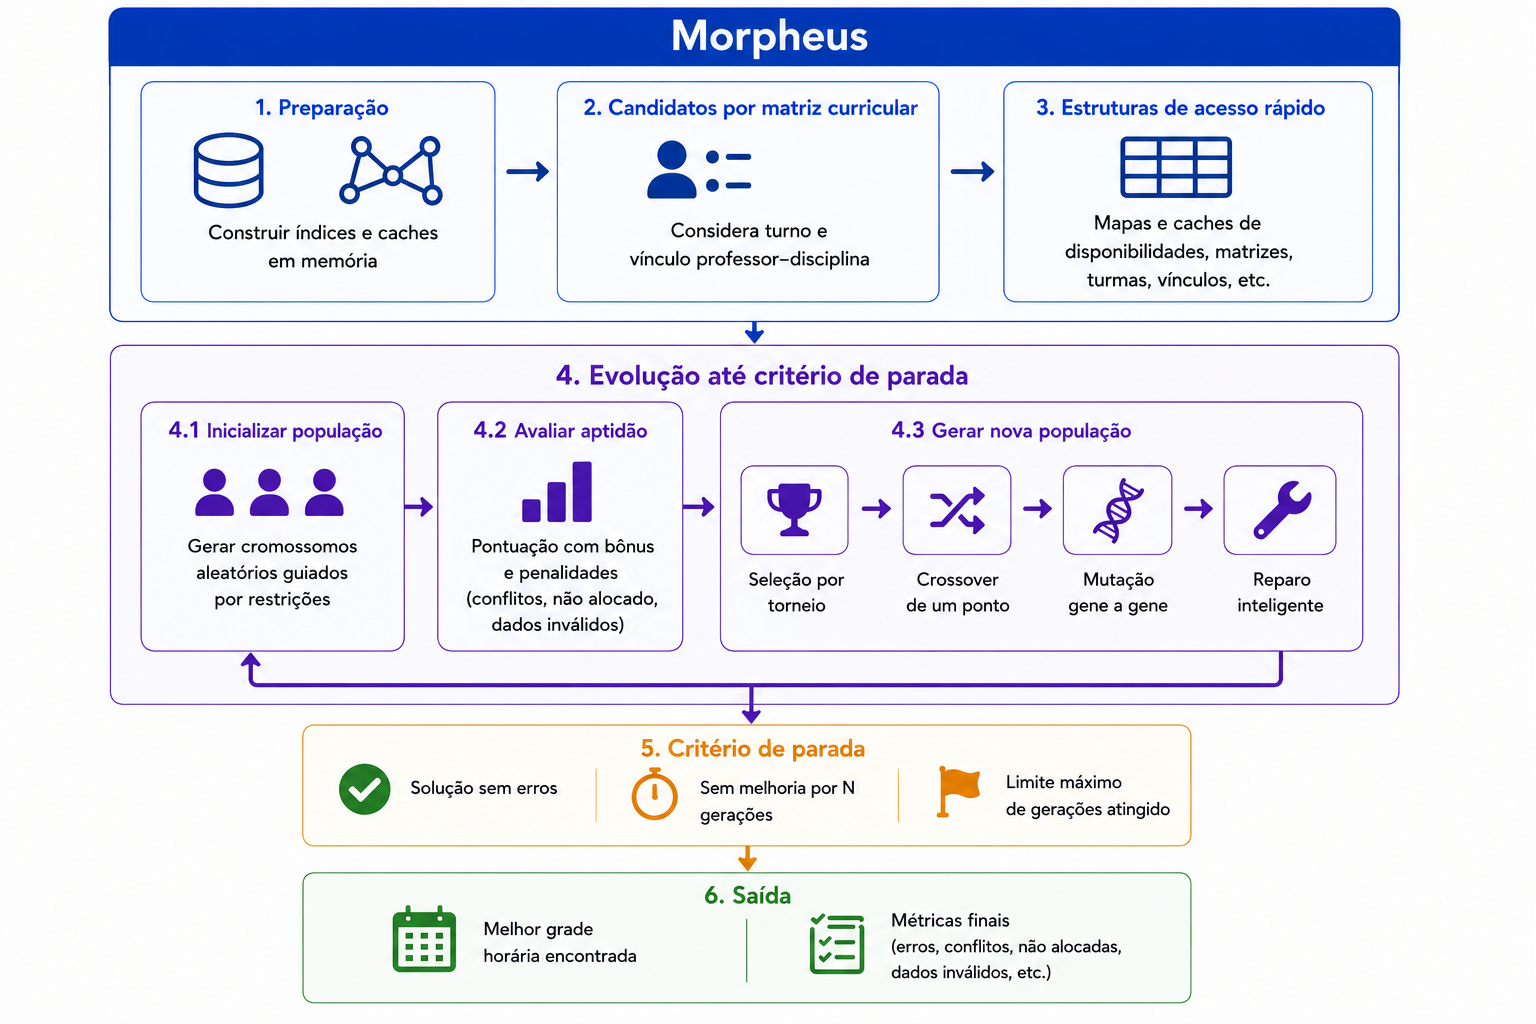
\includegraphics[width=0.85\textwidth]{figuras/Figura_16_ilustracaoFluxoMorpheus.png}

\vspace{0.2cm}
\fonteautores
\end{figure}

\section{Implementação do Algoritmo Rocket}
\label{sec:7.3}

No Rocket, a execução do algoritmo genético ocorre a partir de uma requisição que concentra os dados acadêmicos necessários à geração da grade horária, contendo informações sobre disponibilidades docentes, matrizes curriculares, turmas, vínculos entre professores e disciplinas, parâmetros do algoritmo genético, parâmetros da função \textit{fitness} e, quando necessário, uma URL de callback para envio do resultado.

Antes de iniciar a evolução, o Rocket organiza os dados recebidos por meio da construção de índices auxiliares, criando mapas de acesso rápido para disponibilidades, matrizes, turmas, professores, dias da semana, turnos e vínculos. Entre essas estruturas, destaca-se a lista de candidatos, que armazena para cada matriz curricular quais disponibilidades podem ser utilizadas, considerando o turno da turma e o vínculo entre professor e disciplina.

A representação genética do Rocket difere da utilizada no Sunny e no Morpheus. Enquanto nesses o gene é representado por um par explícito entre matriz e disponibilidade, no Rocket o gene é armazenado como um único valor inteiro correspondente ao identificador de uma disponibilidade. A posição desse gene dentro do cromossomo possui significado próprio: a implementação mantém uma lista ordenada de matrizes, e cada posição do vetor de genes corresponde a uma matriz específica. O valor presente naquela posição indica qual disponibilidade foi atribuída à matriz correspondente. Genes sem alocação recebem o valor unallocatedID = 0.

A população inicial é gerada a partir dos candidatos previamente definidos para cada matriz. Essa geração pode ser classificada como uma inicialização híbrida: a escolha final é aleatória, mas ocorre preferencialmente dentro de um subconjunto menos propenso a conflitos. Quando há alternativas livres para a turma, o sorteio ocorre entre essas opções; quando não há, entre todos os candidatos disponíveis. Um aspecto técnico importante é que a geração da população inicial pode ser paralelizada por meio de \textit{goroutines}, melhorando o desempenho operacional em execuções com populações maiores.

A função \textit{fitness} do Rocket calcula uma pontuação inicial a partir do número total de genes multiplicado pela pontuação base, cujo valor padrão é 10. Além disso, cada alocação válida recebe um bônus adicional de 2 pontos (validBonus) e é aplicado um bônus de diversidade de 5 pontos (diversityBonus) para cada matriz adicional atribuída ao mesmo professor. As penalidades são os elementos mais decisivos: conflito de professor possui o maior peso, com penalidade padrão de 12.000 pontos, refletindo que um docente não pode ministrar duas aulas simultaneamente; conflito de turma recebe penalidade de 8.000 pontos; genes não alocados recebem 10.000 pontos; e dados inválidos ou incompletos também recebem 10.000 pontos. Os pesos são configuráveis por meio dos parâmetros da requisição.

A seleção por torneio cria pressão seletiva moderada. O \textit{crossover} utilizado é de um ponto, implementado de modo que dois pais gerem um novo filho: o algoritmo sorteia um ponto de corte e os genes anteriores a esse ponto são herdados do primeiro pai, enquanto os posteriores são herdados do segundo. A mutação é aplicada gene a gene, selecionando a nova disponibilidade dentro da lista de candidatos válidos para a matriz correspondente.

O reparo do Rocket é implementado como uma tentativa ativa de realocação. O algoritmo calcula ocupações de professor e turma, identifica genes associados a conflitos ou ausência de alocação, e busca a melhor alternativa possível dentro do conjunto de candidatos. A escolha da nova disponibilidade é orientada por uma pontuação interna de conflito: candidatos que colidem com a agenda do professor recebem acréscimo maior, enquanto candidatos que colidem com a agenda da turma recebem acréscimo menor. O algoritmo escolhe o candidato com menor pontuação.

O critério de parada do Rocket combina um limite fixo de gerações com mecanismos de parada antecipada. A execução pode ser interrompida quando uma solução sem erros é encontrada, isto é, quando a melhor grade da geração possui quantidade total de erros igual a zero. Na implementação, esse total corresponde à soma entre disciplinas não alocadas, conflitos de professor, conflitos de turma e dados inválidos ou incompletos. Quando essa condição ocorre, a geração da solução sem erros é registrada e o processo evolutivo é encerrado imediatamente.

Além disso, o Rocket interrompe a evolução quando passa muitas gerações sem melhorar a melhor \textit{fitness} global. O limite de gerações sem melhoria é calculado como 20\% do total de gerações configurado, respeitando um mínimo de 25 e um máximo de 200 gerações, conforme a expressão \texttt{max(25, min(200, numeroGeracoes * 0.20))}. Assim, para 100 gerações configuradas, o limite sem melhoria é 25; para 1.000 gerações, é 200; e para 2.000 gerações, permanece em 200. A melhora considerada nesse critério é uma melhora de \textit{fitness}, não apenas uma redução direta da quantidade de erros. Caso a diferença entre a geração atual e a última geração com melhora alcance esse limite, a execução é interrompida e a resposta indica parada antecipada.

Por fim, se nenhuma das condições anteriores for satisfeita, o algoritmo continua até atingir o número máximo de gerações configurado. O valor padrão utilizado pelo Rocket é de 1.000 gerações, podendo ser sobrescrito na requisição por meio do parâmetro \texttt{numeroGeracoes}. Ao final, o melhor cromossomo é decodificado em uma grade horária e as métricas finais são calculadas, contabilizando disciplinas não alocadas, conflitos de professor, conflitos de turma e dados incompletos, gerando também mensagens textuais de conflito para integração com outros sistemas.

\begin{figure}[H]
\centering
\caption{Fluxo de execução do algoritmo genético Rocket}
\label{fig:fluxo-rocket}

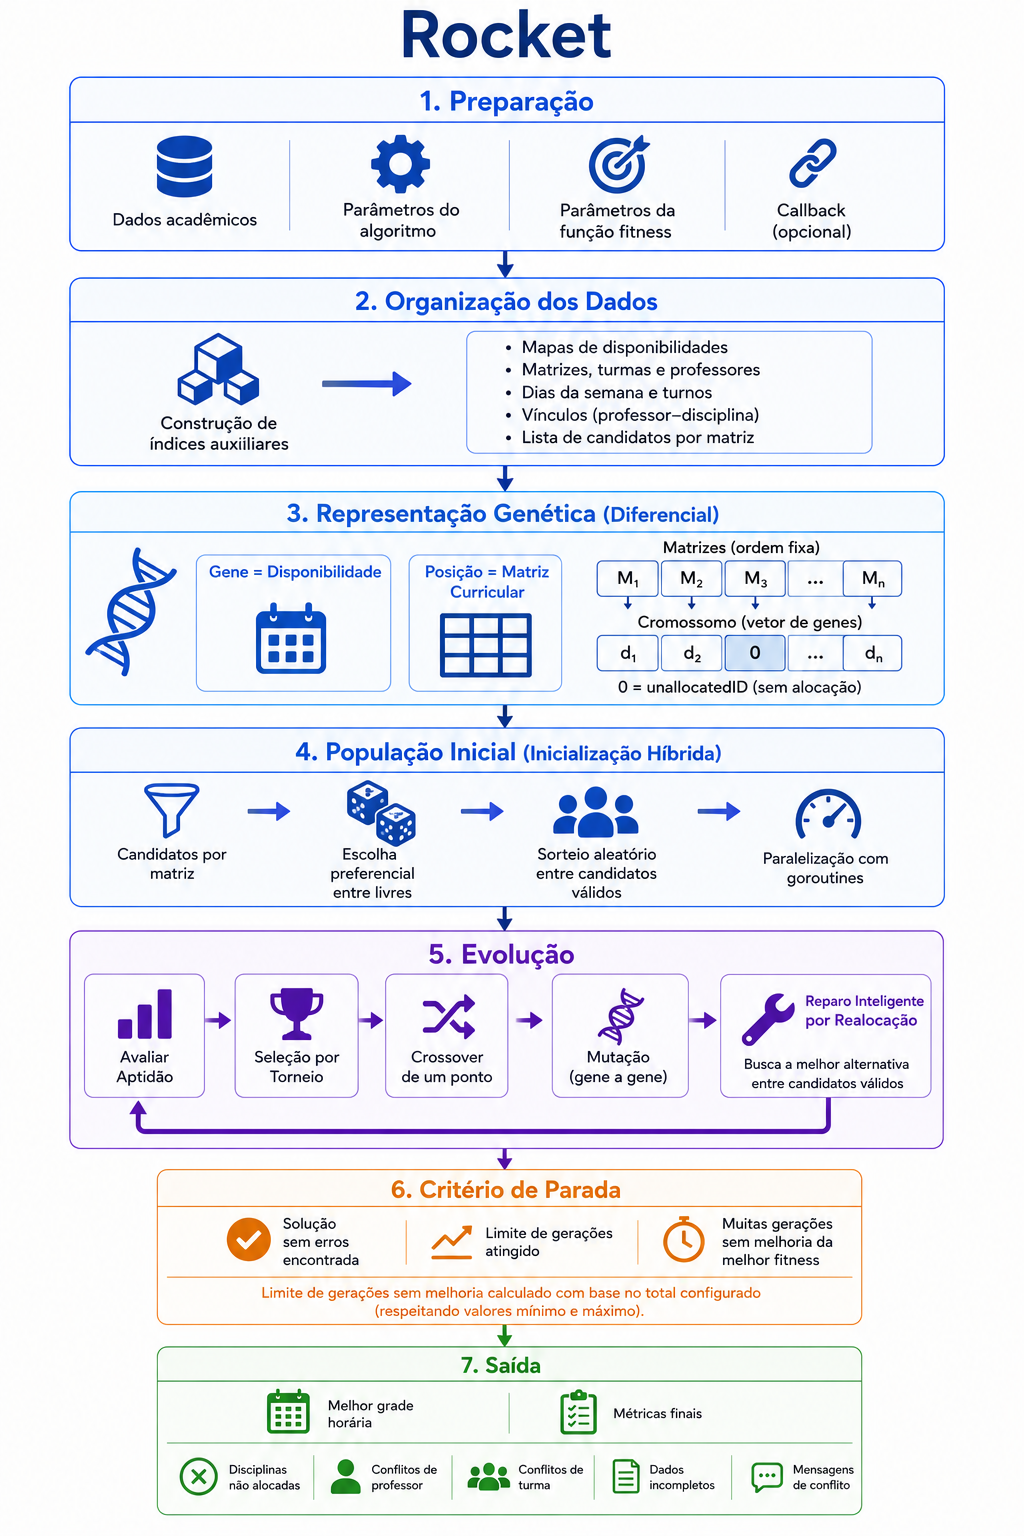
\includegraphics[width=0.85\textwidth]{figuras/Figura_17_ilustracaoFluxoRocket.png}

\vspace{0.2cm}
\fonteautores
\end{figure}


\chapter{Integração e Protótipo Funcional}
\label{cap:integracao}

Este capítulo apresenta os protótipos de interface do sistema IGRIS, desenvolvidos para ilustrar as principais interações dos diferentes perfis de usuário com o sistema. As telas foram projetadas seguindo princípios de usabilidade e experiência do usuário (UI/UX), com foco na clareza das informações e na eficiência operacional dos coordenadores e professores.



\section{Visão Geral das Telas}
\label{sec:9.1}

\newenvironment{tabelainteracoes}[2]{%
\begin{longtable}{|L{4.1cm}|L{5.2cm}|L{5.2cm}|}
\caption{#1}
\label{#2} \\
\hline
\textbf{Comando} & \textbf{Ação} & \textbf{Observações} \\
\hline
\endfirsthead
\hline
\textbf{Comando} & \textbf{Ação} & \textbf{Observações} \\
\hline
\endhead
}{%
\end{longtable}
\fonteautores
}

As telas a seguir demonstram o fluxo completo de uso do sistema IGRIS, desde a autenticação até a visualização da grade gerada pelo algoritmo genético, abrangendo os módulos de gestão acadêmica e o painel docente.

% PG1.jpg
\begin{figure}[H]
\centering
\caption{Tela de Login}
\label{fig:PG1}
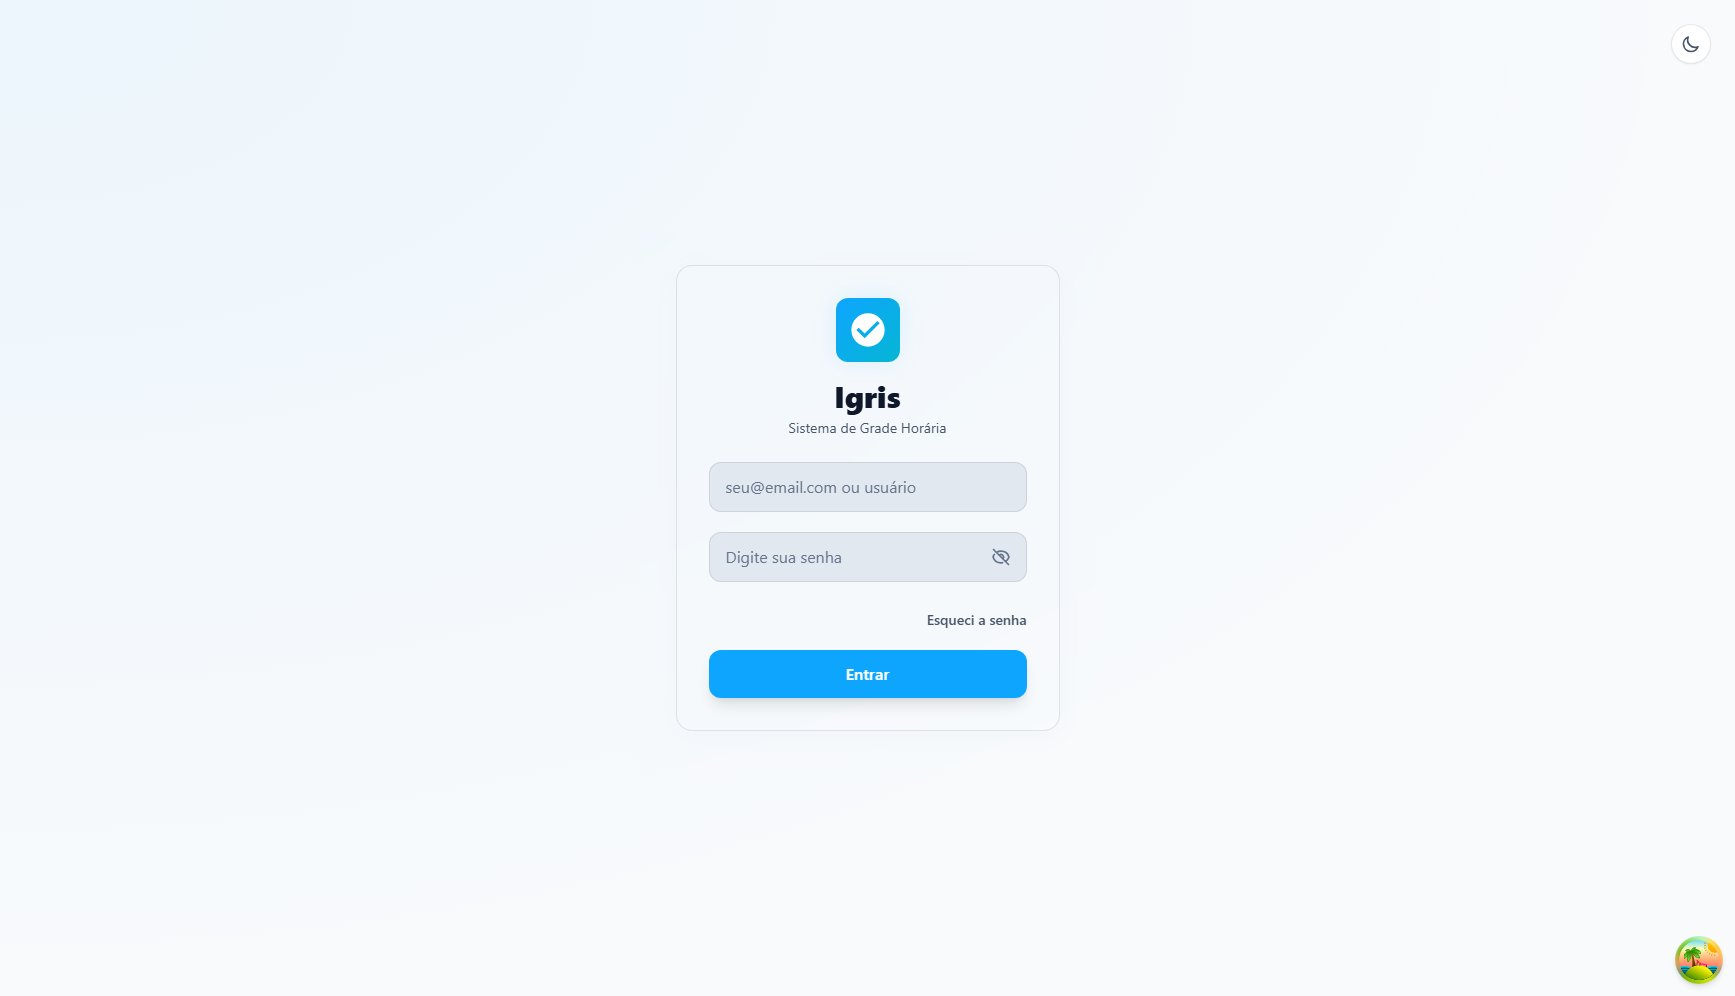
\includegraphics[width=\textwidth]{figuras/paginas/Figura_18_PG1.jpg}
\fonteautores
\end{figure}

A tela de login é o ponto inicial de interação do usuário com o sistema IGRIS. O usuário encontra um formulário composto pelos campos para inserção de e-mail (ou nome de usuário) e senha. A tela também oferece um botão para exibir ou ocultar a senha, a função "Esqueci a senha" e o botão "Entrar" para acessar o sistema. O design em tema escuro com detalhes em azul destaca a modernidade da aplicação.

\begin{longtable}{|L{4.1cm}|L{5.2cm}|L{5.2cm}|}
\caption{Interações da Tela de Login}
\label{tab:interacoes-login} \\
\hline
\textbf{Comando} & \textbf{Ação} & \textbf{Observações} \\
\hline
\endfirsthead
\hline
\textbf{Comando} & \textbf{Ação} & \textbf{Observações} \\
\hline
\endhead
Informar e-mail ou nome de usuário & O sistema registra o identificador digitado para utilizá-lo na autenticação. & O campo é obrigatório e deve corresponder a um usuário previamente cadastrado. \\
\hline
Informar a senha & O sistema mantém o valor digitado oculto e o associa à tentativa de autenticação. & O preenchimento é obrigatório; por segurança, os caracteres são inicialmente representados por pontos. \\
\hline
Clicar no ícone de exibir ou ocultar senha & O sistema alterna a visualização dos caracteres da senha, sem modificar o valor informado. & A função permite conferir a digitação e não interfere nas credenciais enviadas. \\
\hline
Clicar em ``Entrar'' com os campos vazios & O sistema impede o envio do formulário e indica os campos que precisam ser preenchidos. & Deve ser apresentada uma mensagem de obrigatoriedade próxima aos respectivos campos. \\
\hline
Clicar em ``Entrar'' com credenciais inválidas & O sistema rejeita a autenticação e mantém o usuário na tela de login. & A mensagem de erro não deve revelar se o identificador ou a senha está incorreto, preservando a segurança da conta. \\
\hline
Clicar em ``Entrar'' com credenciais válidas & O sistema valida os dados, gera o token de acesso e redireciona o usuário ao ambiente correspondente. & Caso existam múltiplos perfis associados à conta, o usuário deve ser direcionado à tela de seleção de perfil. \\
\hline
Clicar em ``Esqueci a senha'' & O sistema abre a tela de recuperação de senha. & O fluxo seguinte solicita o e-mail associado à conta para o envio do link de recuperação. \\
\hline
Clicar no ícone de alteração de tema & O sistema alterna a aparência da interface entre os temas claro e escuro. & A mudança é apenas visual e não altera os dados preenchidos nem o processo de autenticação. \\
\hline
\end{longtable}

\fonteautores

% PG2.jpg
\begin{figure}[H]
\centering
\caption{Tela de Recuperação de Senha}
\label{fig:PG2}
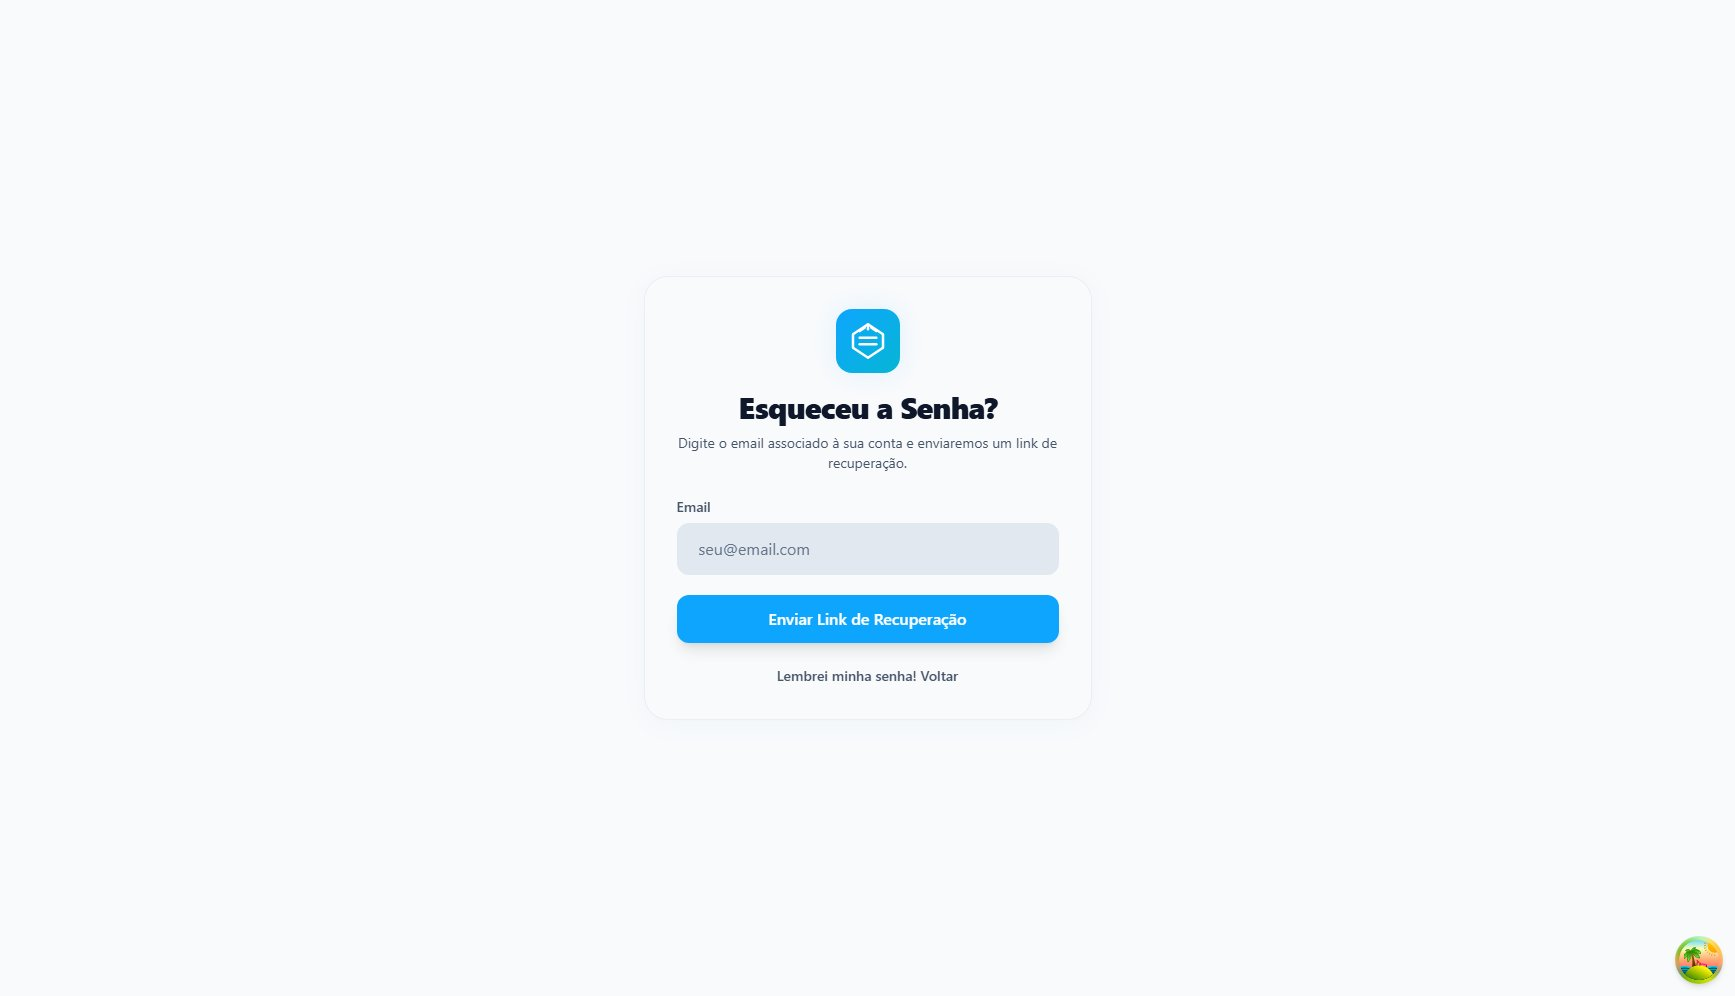
\includegraphics[width=\textwidth]{figuras/paginas/Figura_19_PG2.jpg}
\fonteautores
\end{figure}

A tela de recuperação de senha é acessada pelo link "Esqueci a senha". Nela, o usuário é instruído a digitar o e-mail associado à sua conta para que o sistema envie um link de recuperação. A interface simples e focada fornece os botões "Enviar Link de Recuperação" e um atalho para voltar à tela de login.

\begin{tabelainteracoes}{Interações da Tela de Recuperação de Senha}{tab:interacoes-recuperacao-senha}
Informar o e-mail da conta & O sistema registra o endereço para localizar o cadastro e preparar a solicitação de recuperação. & O campo é obrigatório e deve possuir formato de e-mail válido. \\
\hline
Clicar em ``Enviar Link de Recuperação'' com o campo vazio ou inválido & O sistema não envia a solicitação e informa que o e-mail precisa ser corrigido. & A validação deve ocorrer antes da comunicação com o serviço de recuperação. \\
\hline
Clicar em ``Enviar Link de Recuperação'' com um e-mail válido & O sistema gera um token temporário e envia ao endereço informado as instruções para definição de uma nova senha. & Por segurança, a confirmação não deve revelar se o e-mail está ou não cadastrado. O link deve possuir prazo de validade e uso único. \\
\hline
Clicar em ``Lembrei minha senha! Voltar'' & O sistema encerra o fluxo de recuperação e retorna à tela de login. & Nenhuma solicitação é criada e o e-mail digitado pode ser descartado. \\
\hline
Utilizar um link expirado ou já usado & O sistema recusa a redefinição e orienta o usuário a solicitar um novo link. & O token de recuperação deve ser validado antes de permitir a alteração da senha. \\
\hline
\end{tabelainteracoes}

% PG3.jpg
\begin{figure}[H]
\centering
\caption{Tela de Seleção de Perfil}
\label{fig:PG3}
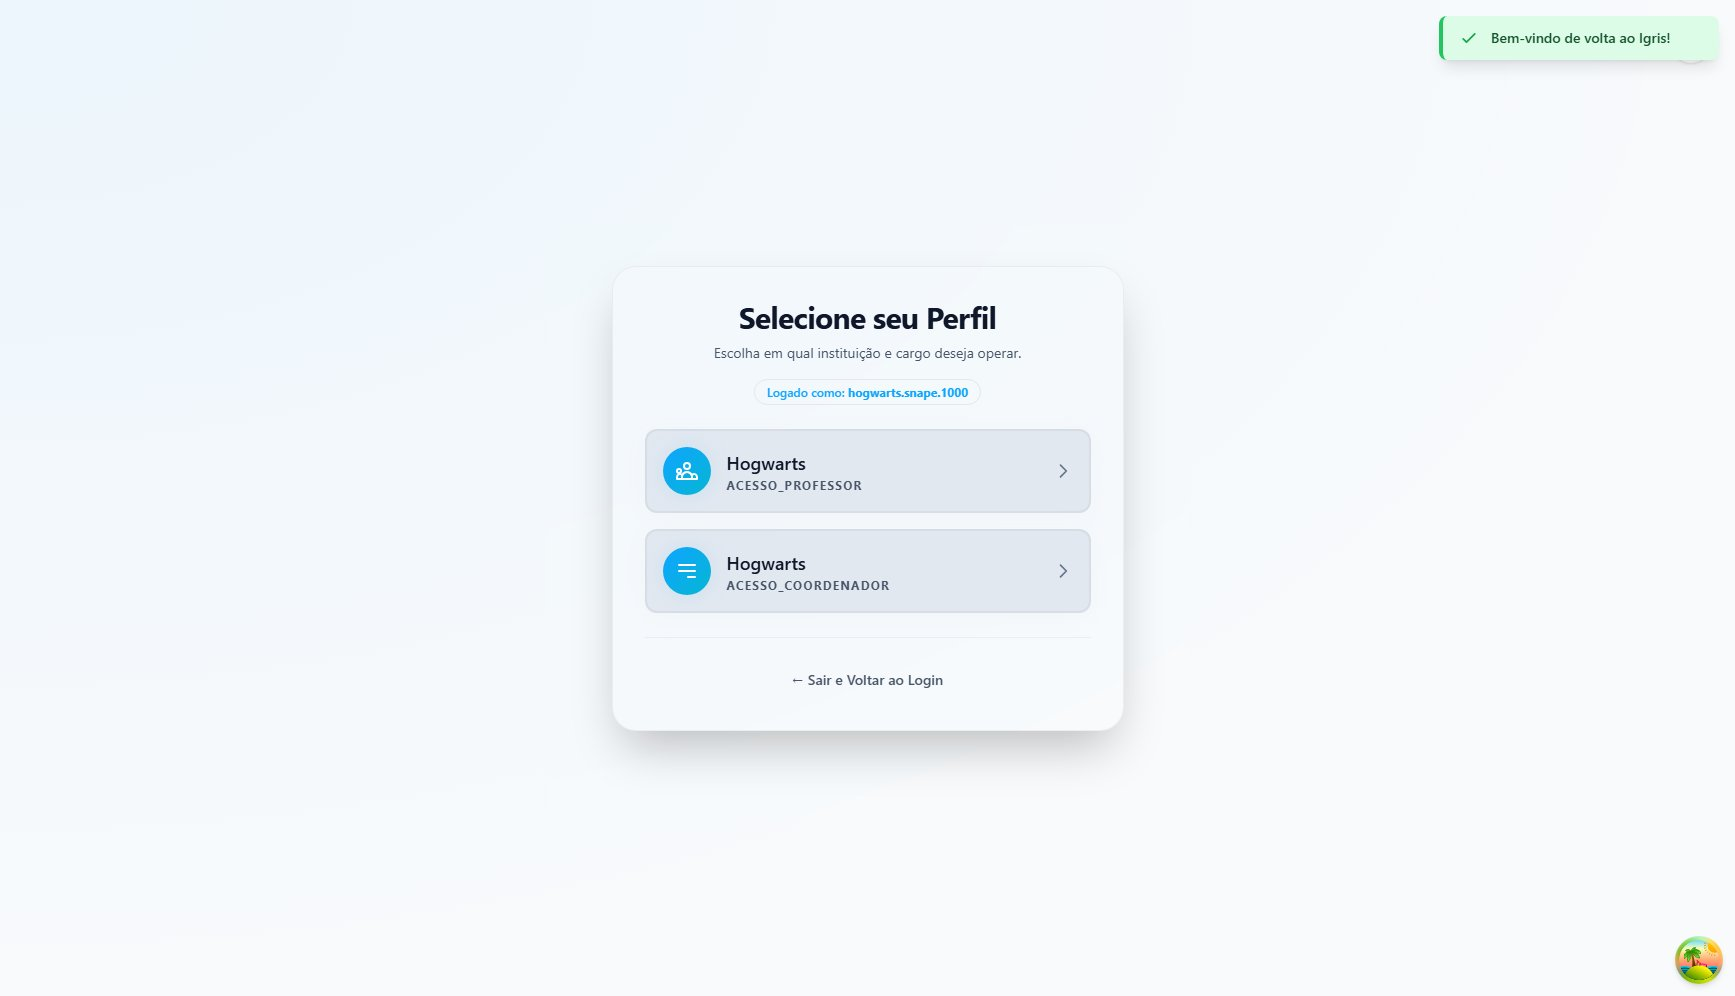
\includegraphics[width=\textwidth]{figuras/paginas/Figura_20_PG3.jpg}
\fonteautores
\end{figure}

Após a autenticação, se o usuário possuir mais de um papel, é apresentada a tela de seleção de perfil. Essa interface exibe as instituições e cargos disponíveis, como \texttt{ACESSO\_\allowbreak COORDENADOR} e \texttt{ACESSO\_\allowbreak PROFESSOR}, permitindo que o usuário direcione sua navegação ao ambiente adequado. Também há uma opção para sair e voltar ao login.

\begin{tabelainteracoes}{Interações da Tela de Seleção de Perfil}{tab:interacoes-selecao-perfil}
Visualizar os perfis disponíveis & O sistema lista somente os perfis e instituições vinculados à conta autenticada. & Cada opção deve identificar o contexto institucional e o nível de acesso correspondente. \\
\hline
Clicar em um perfil & O sistema ativa o contexto selecionado, emite um novo token de acesso e direciona o usuário ao painel adequado. & As permissões e funcionalidades exibidas passam a respeitar o perfil escolhido. \\
\hline
Selecionar um perfil sem vínculo válido ou inativo & O sistema impede o acesso e informa que o perfil não está disponível. & O vínculo deve ser validado novamente no servidor, mesmo que apareça previamente na interface. \\
\hline
Clicar em ``Sair e Voltar ao Login'' & O sistema encerra a sessão atual e apresenta novamente a tela de autenticação. & Tokens e dados temporários da sessão devem ser invalidados. \\
\hline
\end{tabelainteracoes}

% PG4.jpg
\begin{figure}[H]
\centering
\caption{Painel do Coordenador - Visão Geral}
\label{fig:PG4}
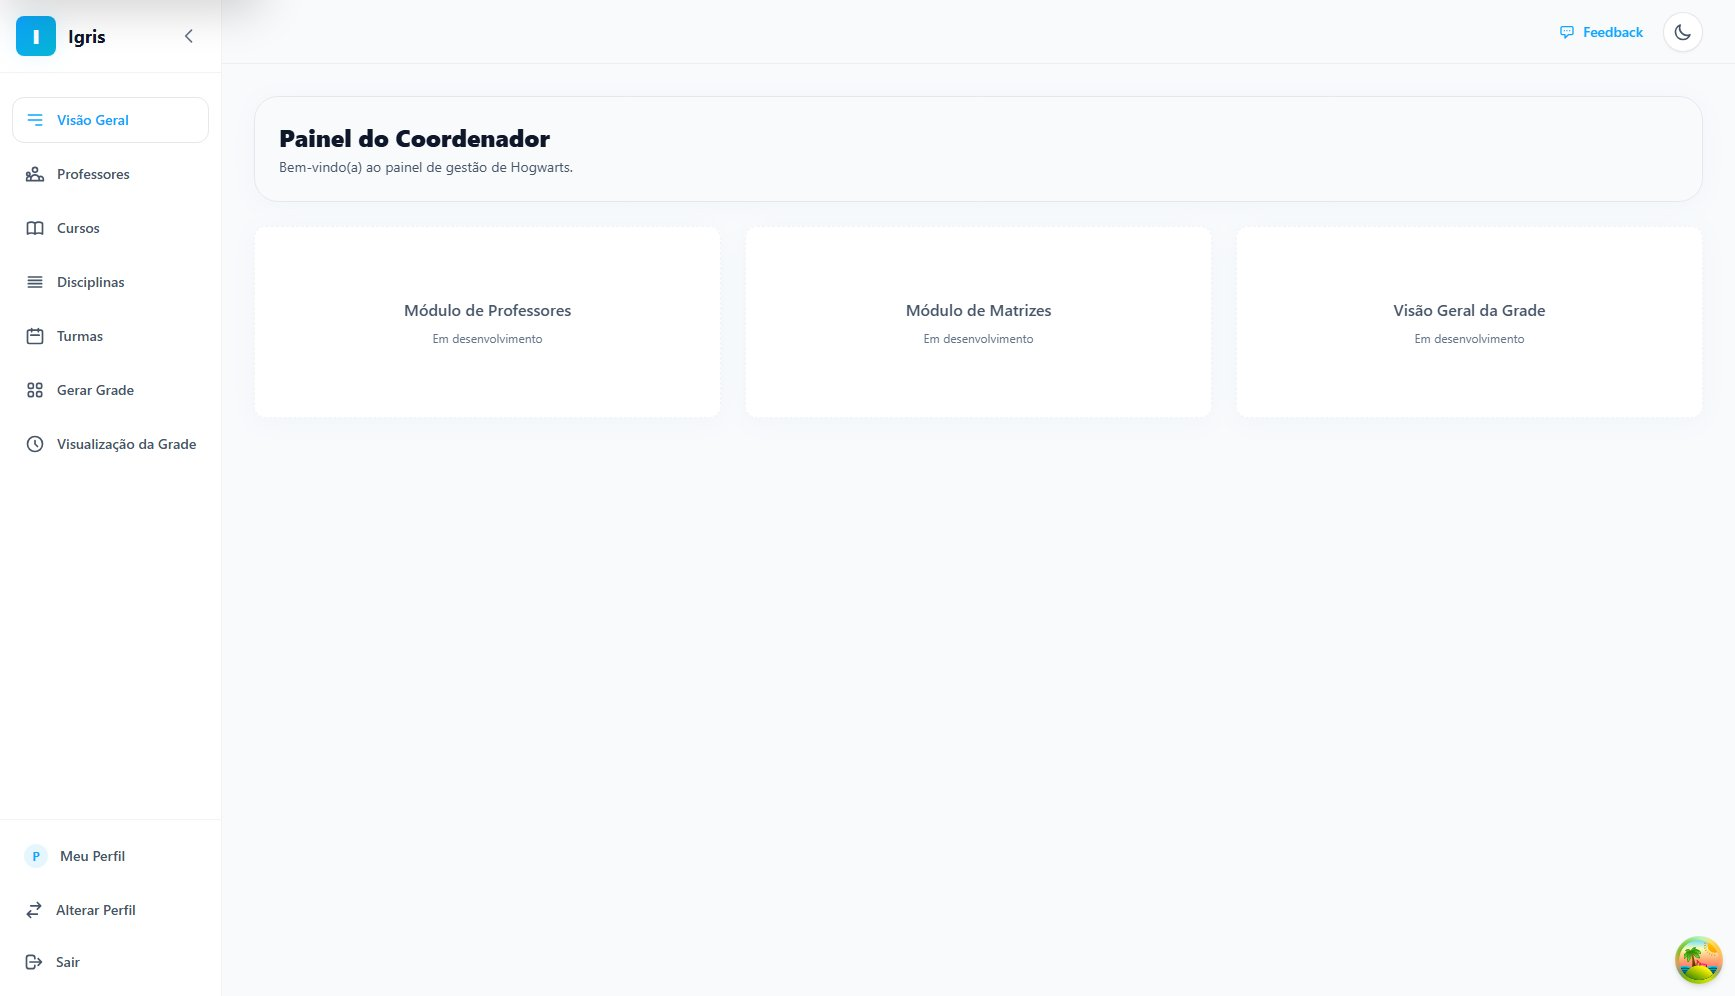
\includegraphics[width=\textwidth]{figuras/paginas/Figura_21_PG4.jpg}
\fonteautores
\end{figure}

O Painel do Coordenador apresenta a interface principal do gestor acadêmico. Um menu lateral à esquerda fornece acesso rápido às seções essenciais do sistema: Professores, Cursos, Disciplinas, Turmas, Gerar Grade e Visualização da Grade, centralizando o controle da grade horária da instituição.

\begin{tabelainteracoes}{Interações do Painel do Coordenador}{tab:interacoes-painel-coordenador}
Clicar em uma opção do menu lateral & O sistema abre o módulo correspondente e destaca a seção ativa. & Apenas módulos autorizados para o perfil de coordenador devem permanecer disponíveis. \\
\hline
Clicar em um cartão de acesso rápido & O sistema direciona o usuário ao módulo indicado, como Professores, Matrizes ou Visualização da Grade. & O cartão funciona como atalho e deve produzir o mesmo resultado da opção equivalente no menu. \\
\hline
Clicar em ``Meu Perfil'' & O sistema abre as informações e configurações da conta do usuário. & Alterações pessoais não devem modificar automaticamente o perfil institucional ativo. \\
\hline
Clicar em ``Alterar Perfil'' & O sistema retorna à seleção de perfil para que outro vínculo seja ativado. & Ao confirmar a troca, as permissões e o contexto institucional devem ser recarregados. \\
\hline
Clicar em ``Sair'' & O sistema encerra a sessão e retorna à tela de login. & O token de acesso deve ser invalidado ou removido do cliente. \\
\hline
\end{tabelainteracoes}

% PG5.jpg
\begin{figure}[H]
\centering
\caption{Tela de Gerenciamento de Corpo Docente}
\label{fig:PG5}
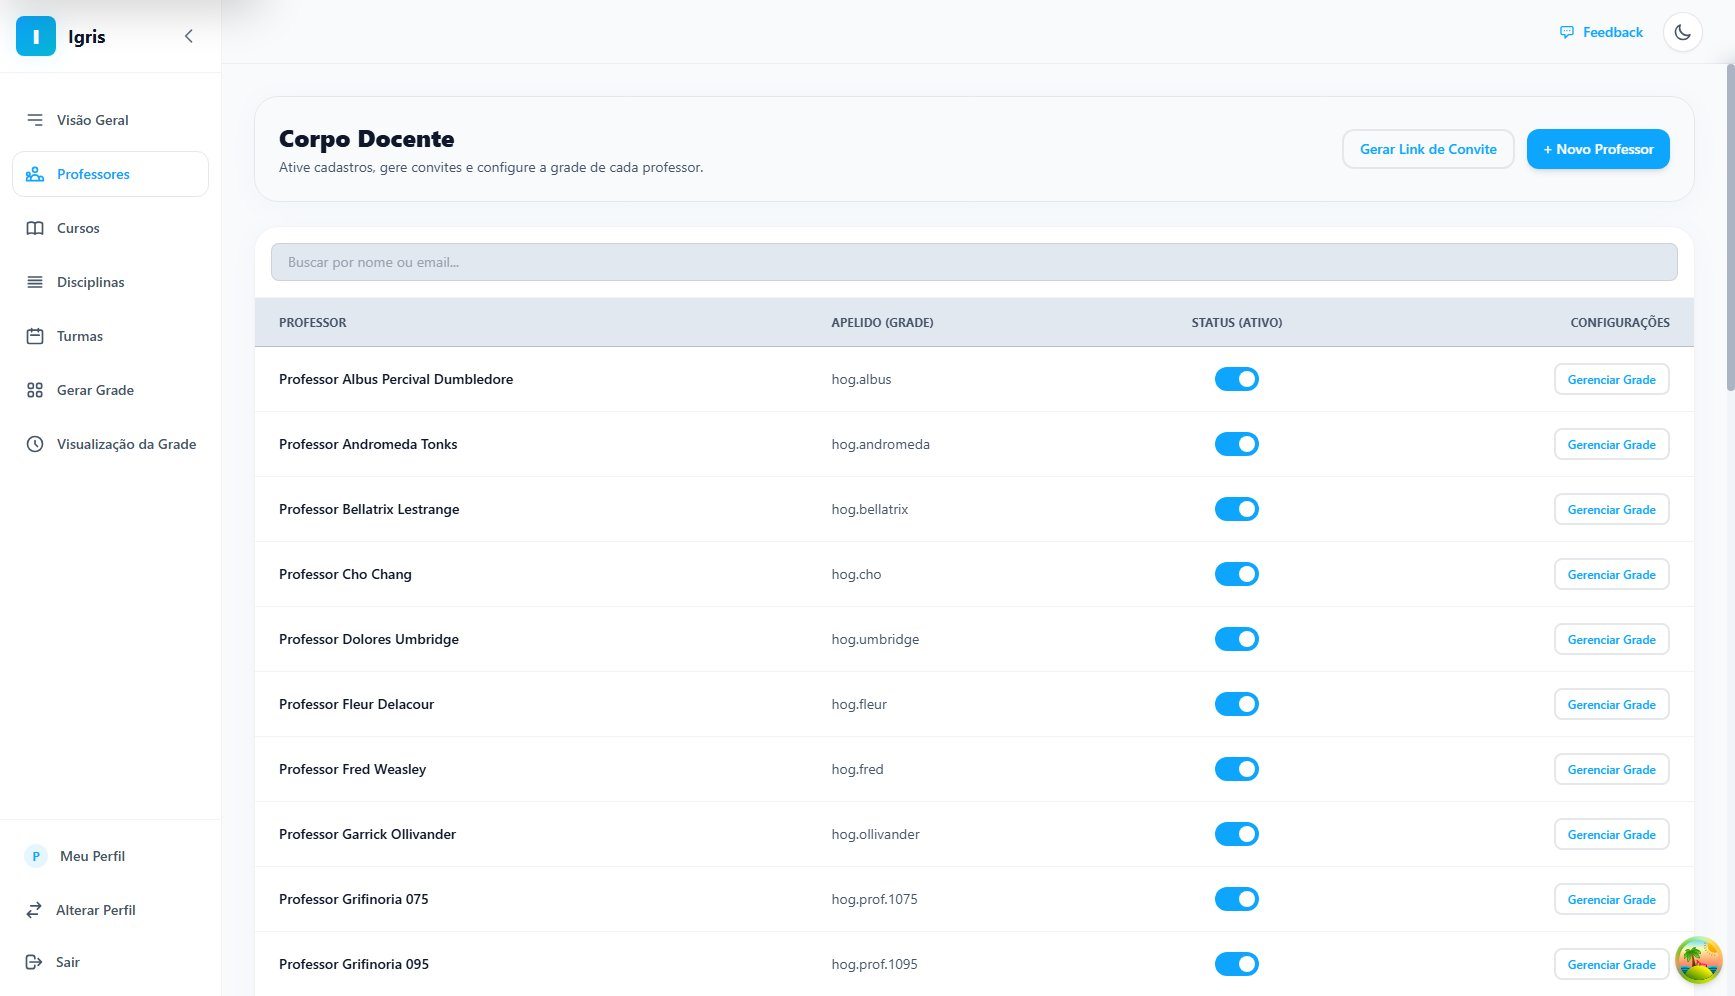
\includegraphics[width=\textwidth]{figuras/paginas/Figura_22_PG5.jpg}
\fonteautores
\end{figure}

Na tela de professores, o coordenador pode visualizar e gerenciar o corpo docente. O sistema apresenta uma lista com o nome, e-mail/login e status de cada professor. Interruptores de ativação (toggles) permitem habilitar ou desabilitar o acesso dos docentes ao sistema rapidamente, além de oferecer botões para gerenciar a grade individual de cada um.

\begin{tabelainteracoes}{Interações da Tela de Gerenciamento de Corpo Docente}{tab:interacoes-corpo-docente}
Pesquisar pelo nome ou e-mail do professor & O sistema filtra a listagem conforme o texto informado. & Quando não houver correspondências, deve ser exibida uma indicação de lista vazia. \\
\hline
Alterar o interruptor de status & O sistema ativa ou desativa o acesso do professor e atualiza o estado apresentado na lista. & A desativação impede novos acessos, mas não deve excluir o cadastro nem os vínculos acadêmicos existentes. \\
\hline
Clicar em ``Gerenciar Grade'' & O sistema abre as configurações de áreas de atuação e disponibilidade do professor selecionado. & As alterações devem afetar somente o docente correspondente à linha acionada. \\
\hline
Clicar em ``Gerar Link de Convite'' & O sistema cria um convite seguro para o autocadastro de um novo professor. & O link deve possuir token único, prazo de validade e associação com a instituição. \\
\hline
Clicar em ``Novo Professor'' & O sistema abre o formulário de cadastro manual de docente. & Somente usuários autorizados podem criar ou ativar professores. \\
\hline
\end{tabelainteracoes}

% PG6.jpg
\begin{figure}[H]
\centering
\caption{Geração de Link de Convite para Docentes}
\label{fig:PG6}
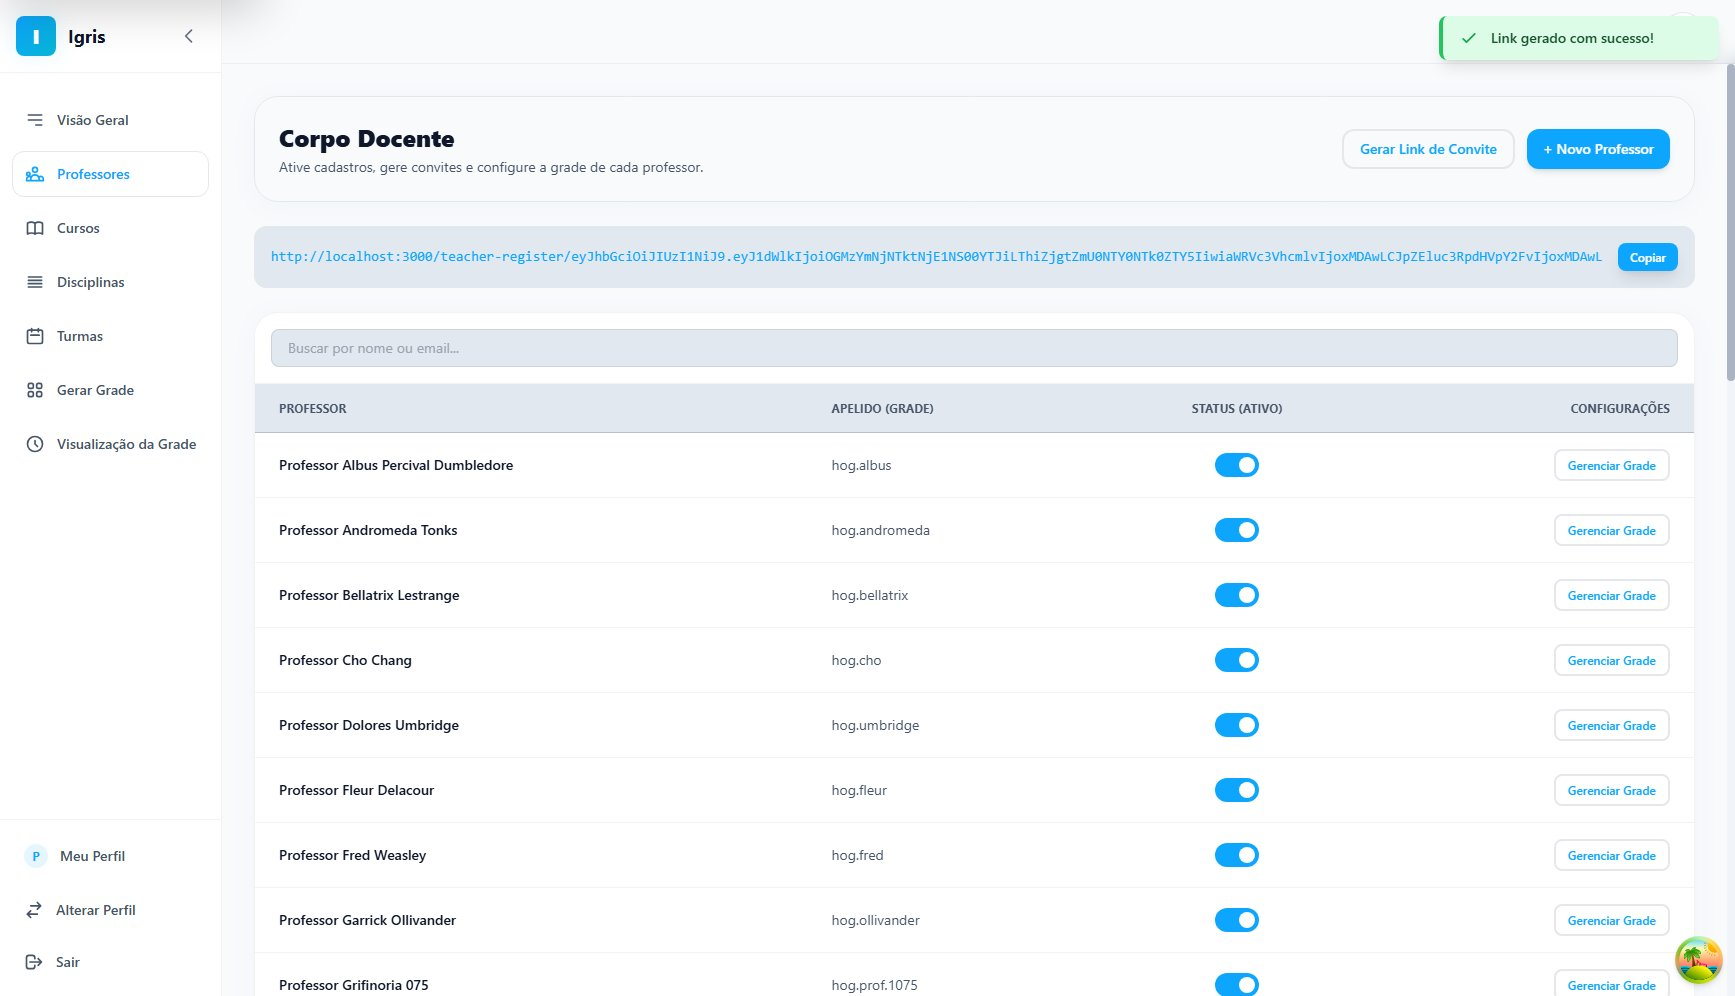
\includegraphics[width=\textwidth]{figuras/paginas/Figura_23_PG6.jpg}
\fonteautores
\end{figure}

A tela do corpo docente também permite a geração de um link de convite. Ao clicar no botão correspondente, o sistema cria e exibe uma URL específica que pode ser copiada e compartilhada com os professores, facilitando o auto-cadastramento deles na plataforma institucional.

\begin{tabelainteracoes}{Interações da Geração de Link de Convite}{tab:interacoes-link-convite-docente}
Clicar em ``Gerar Link de Convite'' & O sistema cria um token seguro e apresenta a URL de cadastro na própria tela. & O convite deve estar vinculado à instituição e ao perfil de professor. \\
\hline
Clicar em ``Copiar'' & O sistema envia a URL exibida para a área de transferência e confirma a operação. & A cópia não altera a validade nem permite a reutilização de um convite já consumido. \\
\hline
Compartilhar e acessar o link válido & O sistema abre o formulário de autocadastro e associa o novo usuário ao contexto do convite. & Após a conclusão do cadastro, o token deve expirar para impedir novos usos. \\
\hline
Acessar um convite inválido ou expirado & O sistema bloqueia o cadastro e informa que um novo convite deve ser solicitado. & Nenhum perfil ou vínculo institucional deve ser criado nessa situação. \\
\hline
Solicitar a geração de outro link & O sistema cria uma nova URL, independente da anterior. & Conforme a regra adotada, o convite anterior pode ser invalidado para reduzir o risco de uso indevido. \\
\hline
\end{tabelainteracoes}

% PG7.jpg
\begin{figure}[H]
\centering
\caption{Tela de Cadastro de Novo Professor}
\label{fig:PG7}
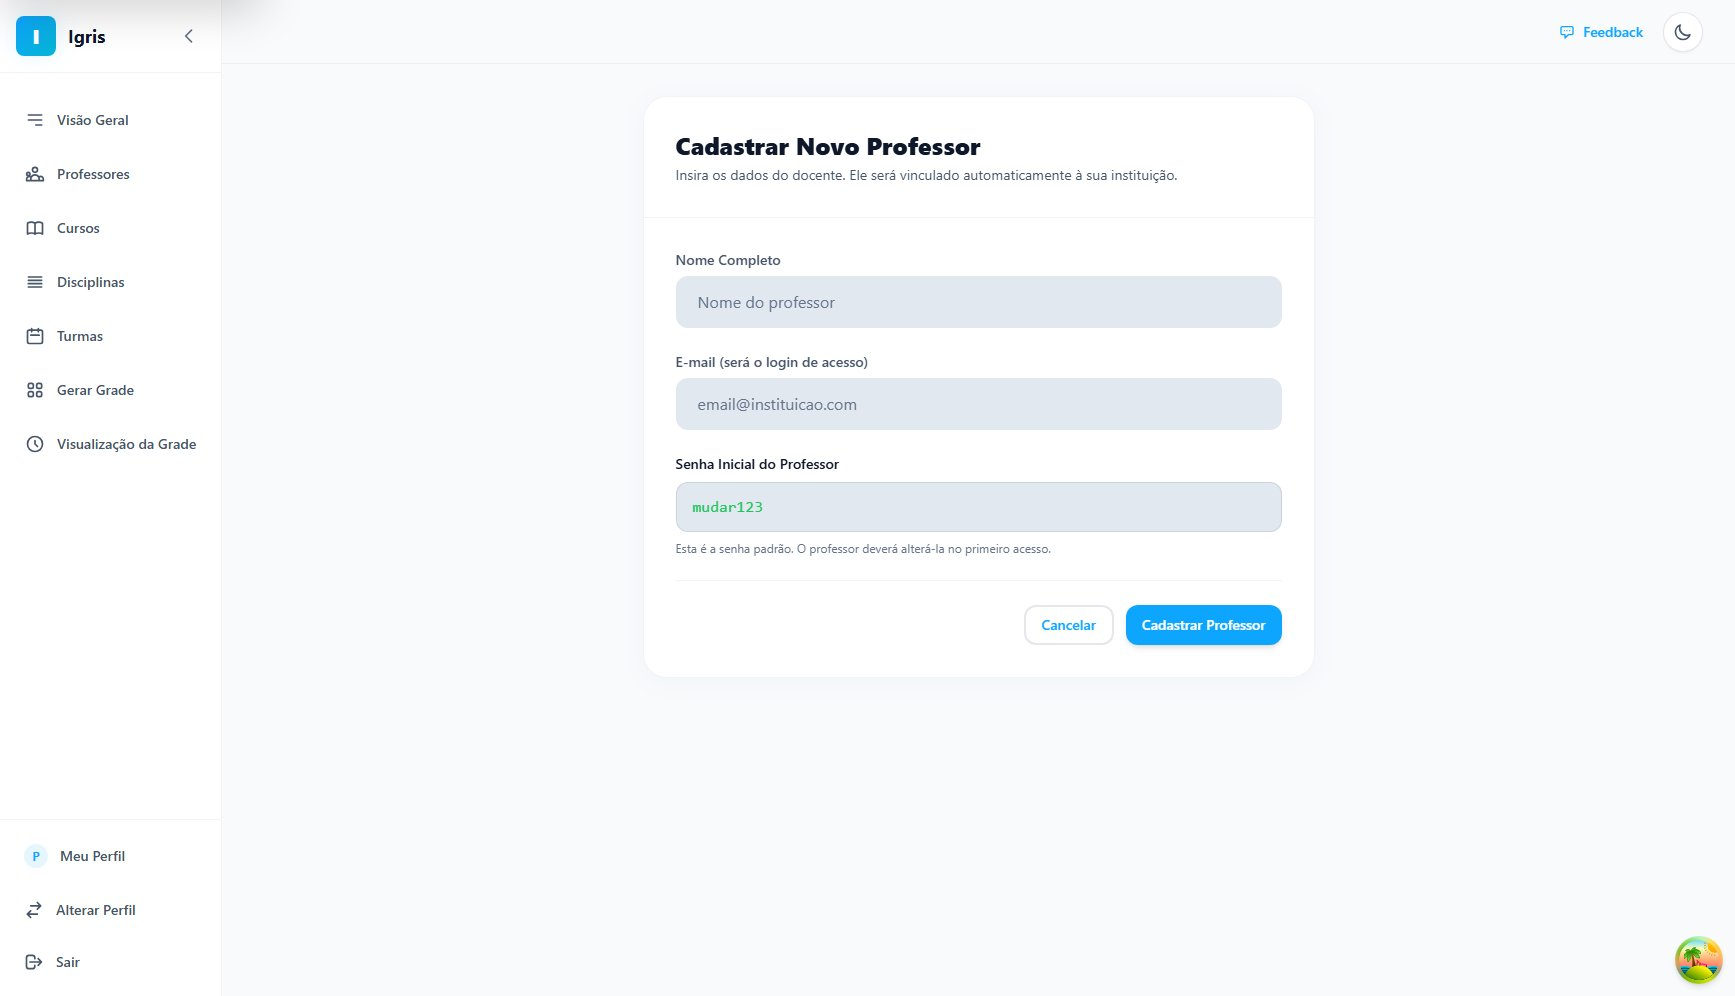
\includegraphics[width=\textwidth]{figuras/paginas/Figura_24_PG7.jpg}
\fonteautores
\end{figure}

Acessada pelo botão "Novo Professor", esta janela em formato de sobreposição (modal) permite o cadastro manual de um docente. O coordenador insere o nome, e-mail e uma senha inicial padrão que o professor deverá alterar posteriormente em seu primeiro acesso.

\begin{tabelainteracoes}{Interações da Tela de Cadastro de Novo Professor}{tab:interacoes-cadastro-professor}
Informar o nome completo & O sistema registra o nome que identificará o docente nas listagens e grades. & O campo é obrigatório e não deve aceitar apenas espaços em branco. \\
\hline
Informar o e-mail ou login & O sistema utiliza o valor como identificador de acesso do professor. & O endereço deve possuir formato válido e não pode estar associado a outro usuário. \\
\hline
Informar a senha inicial & O sistema oculta os caracteres e prepara a senha para armazenamento seguro. & Devem ser aplicadas as regras mínimas de segurança; a senha precisa ser criptografada e alterada no primeiro acesso. \\
\hline
Clicar em ``Cadastrar Professor'' com dados válidos & O sistema cria o usuário, vincula o perfil de professor e fecha o formulário. & A listagem deve ser atualizada e uma mensagem de sucesso apresentada. \\
\hline
Clicar em ``Cadastrar Professor'' com dados inválidos & O sistema mantém o formulário aberto e destaca os campos que precisam de correção. & O cadastro não pode ser criado parcialmente. \\
\hline
Clicar em ``Cancelar'' ou no ícone de fechar & O sistema fecha a janela sem salvar o novo professor. & Se houver dados preenchidos, eles são descartados. \\
\hline
\end{tabelainteracoes}

% PG8.jpg
\begin{figure}[H]
\centering
\caption{Tela de Gerenciamento de Turmas}
\label{fig:PG8}
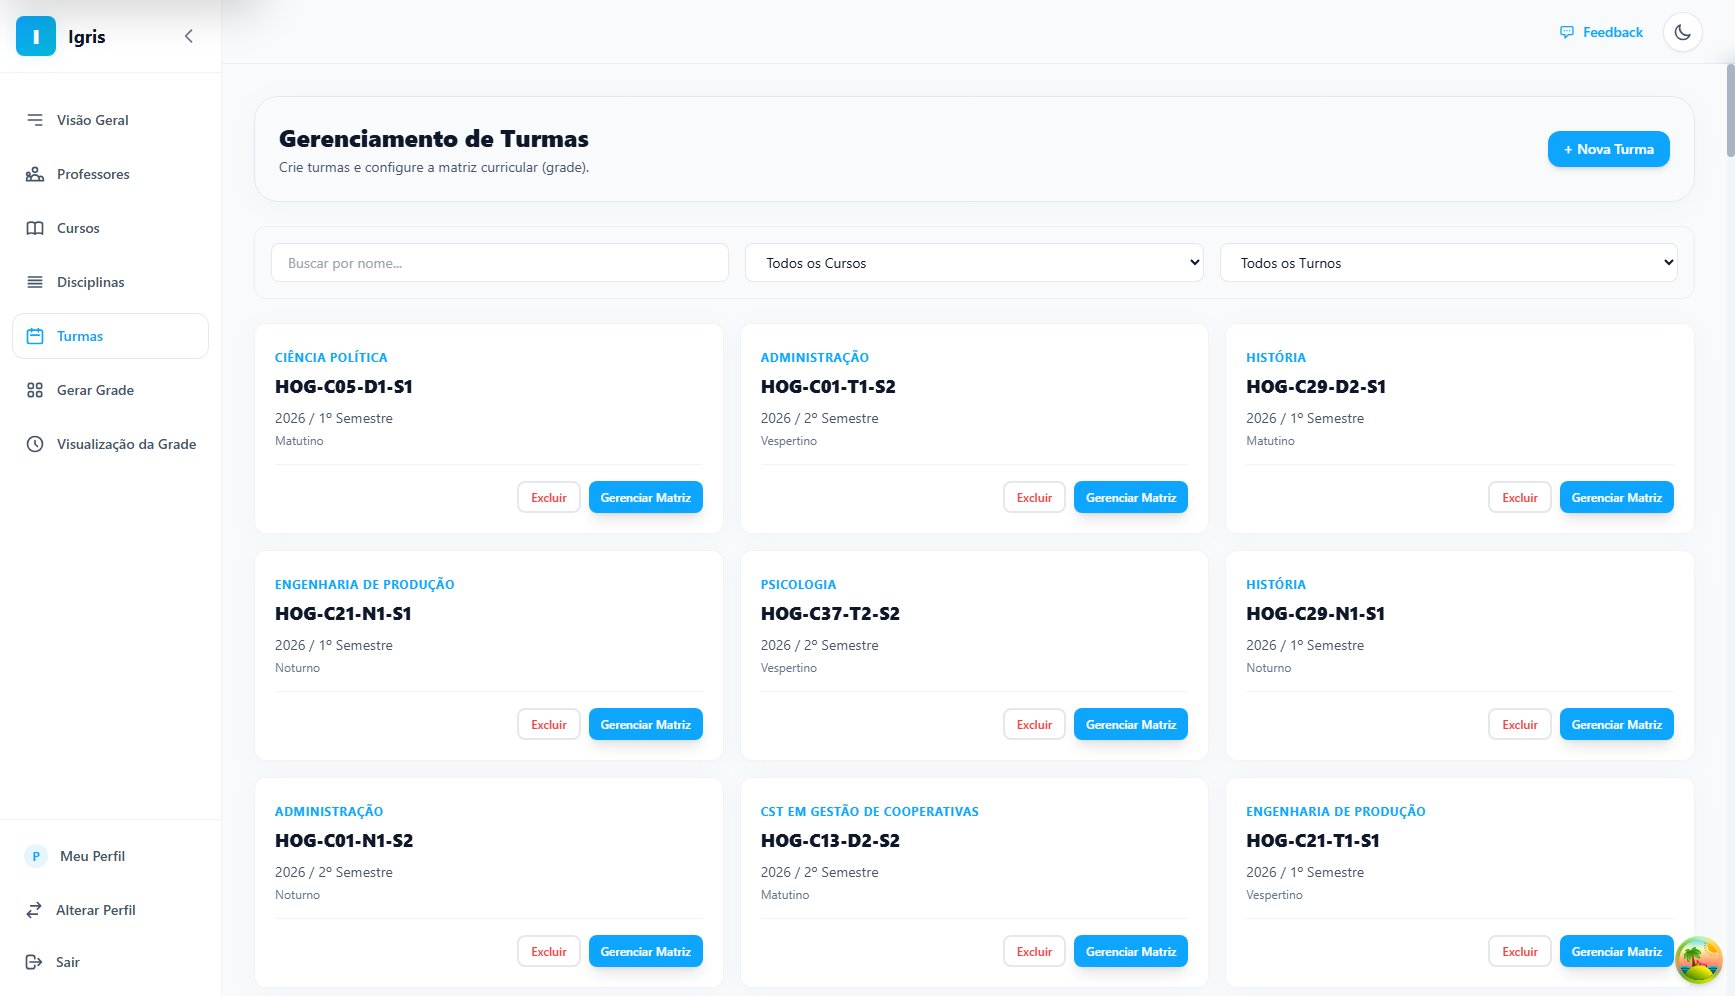
\includegraphics[width=\textwidth]{figuras/paginas/Figura_25_PG8.jpg}
\fonteautores
\end{figure}

A tela de Gerenciamento de Turmas apresenta todas as turmas cadastradas organizadas em cartões. O coordenador pode visualizar dados como curso associado, turno (matutino, vespertino, noturno) e período letivo. Estão disponíveis ferramentas de busca, filtros e botões para gerenciar a matriz de cada turma, além de uma opção para criar novas turmas.

\begin{tabelainteracoes}{Interações da Tela de Gerenciamento de Turmas}{tab:interacoes-gerenciamento-turmas}
Pesquisar uma turma pelo nome & O sistema filtra os cartões enquanto o usuário informa o termo de busca. & A busca deve considerar o identificador ou nome apresentado no cartão. \\
\hline
Selecionar os filtros de curso ou turno & O sistema restringe a listagem às turmas compatíveis com os critérios escolhidos. & Os filtros podem ser combinados e devem permitir o retorno à opção de exibir todos os registros. \\
\hline
Clicar em ``Gerenciar Matriz'' & O sistema abre a janela com os dados e as disciplinas vinculadas à turma selecionada. & A operação deve manter o contexto da turma acionada. \\
\hline
Clicar em ``Excluir'' & O sistema solicita confirmação e, se autorizado, remove a turma. & A exclusão deve ser bloqueada ou tratada quando existirem matrizes, grades ou alocações dependentes. \\
\hline
Clicar em ``Nova Turma'' & O sistema abre o formulário para criação de uma turma e de sua matriz inicial. & O novo registro deve ficar vinculado à coordenação ativa. \\
\hline
\end{tabelainteracoes}

% PG9.jpg
\begin{figure}[H]
\centering
\caption{Catálogo de Cursos}
\label{fig:PG9}
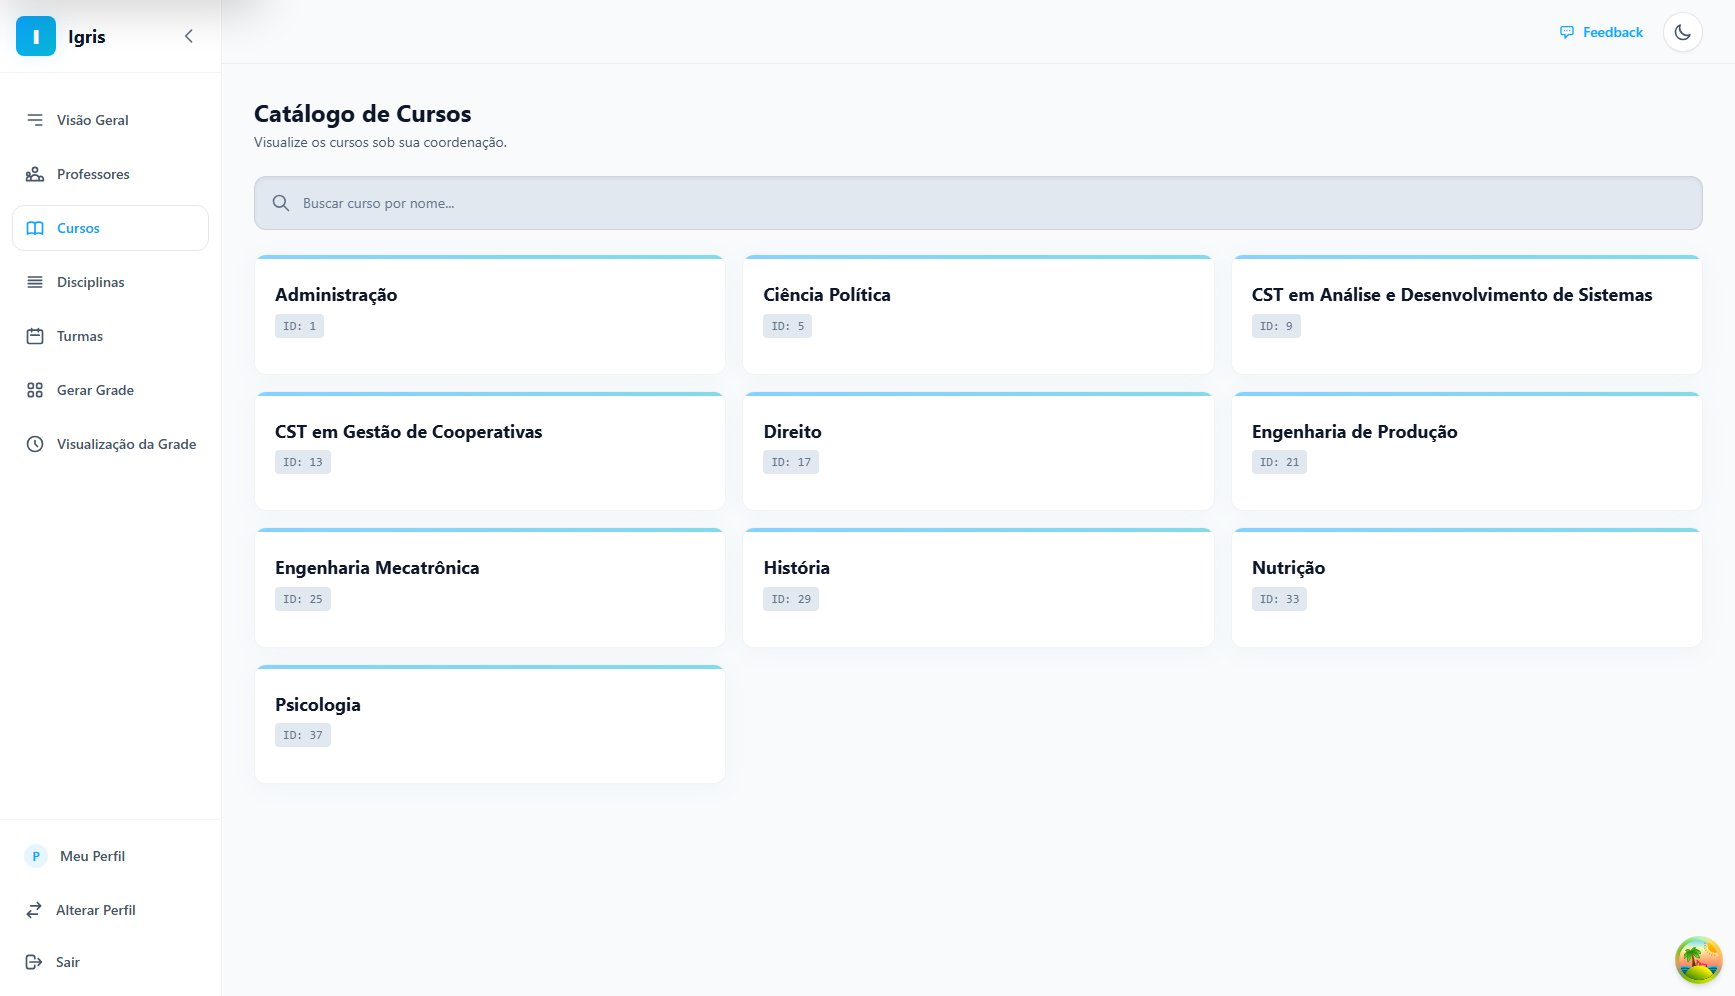
\includegraphics[width=\textwidth]{figuras/paginas/Figura_26_PG9.jpg}
\fonteautores
\end{figure}

A tela de cursos exibe as formações acadêmicas disponíveis sob a coordenação do usuário. Cada curso é representado por um cartão interativo contendo seu nome e identificador interno, fornecendo uma base estrutural para a criação de turmas e atribuição de disciplinas.

\begin{tabelainteracoes}{Interações do Catálogo de Cursos}{tab:interacoes-catalogo-cursos}
Pesquisar pelo nome do curso & O sistema filtra os cartões e exibe somente os cursos correspondentes. & A pesquisa deve aceitar correspondências parciais e informar quando nenhum resultado for encontrado. \\
\hline
Visualizar um cartão de curso & O sistema apresenta o nome e o identificador interno do registro. & Devem ser listados apenas os cursos pertencentes ao contexto institucional do coordenador. \\
\hline
Clicar em um cartão de curso & O sistema seleciona ou abre os detalhes do curso, conforme a operação disponível no módulo. & O curso serve de referência para turmas, matrizes e vínculos de disciplinas. \\
\hline
Tentar acessar um curso sem permissão & O sistema recusa a operação e mantém o usuário no catálogo autorizado. & A autorização deve ser verificada no servidor, e não apenas pela interface. \\
\hline
\end{tabelainteracoes}

% PG10.jpg
\begin{figure}[H]
\centering
\caption{Catálogo de Disciplinas}
\label{fig:PG10}
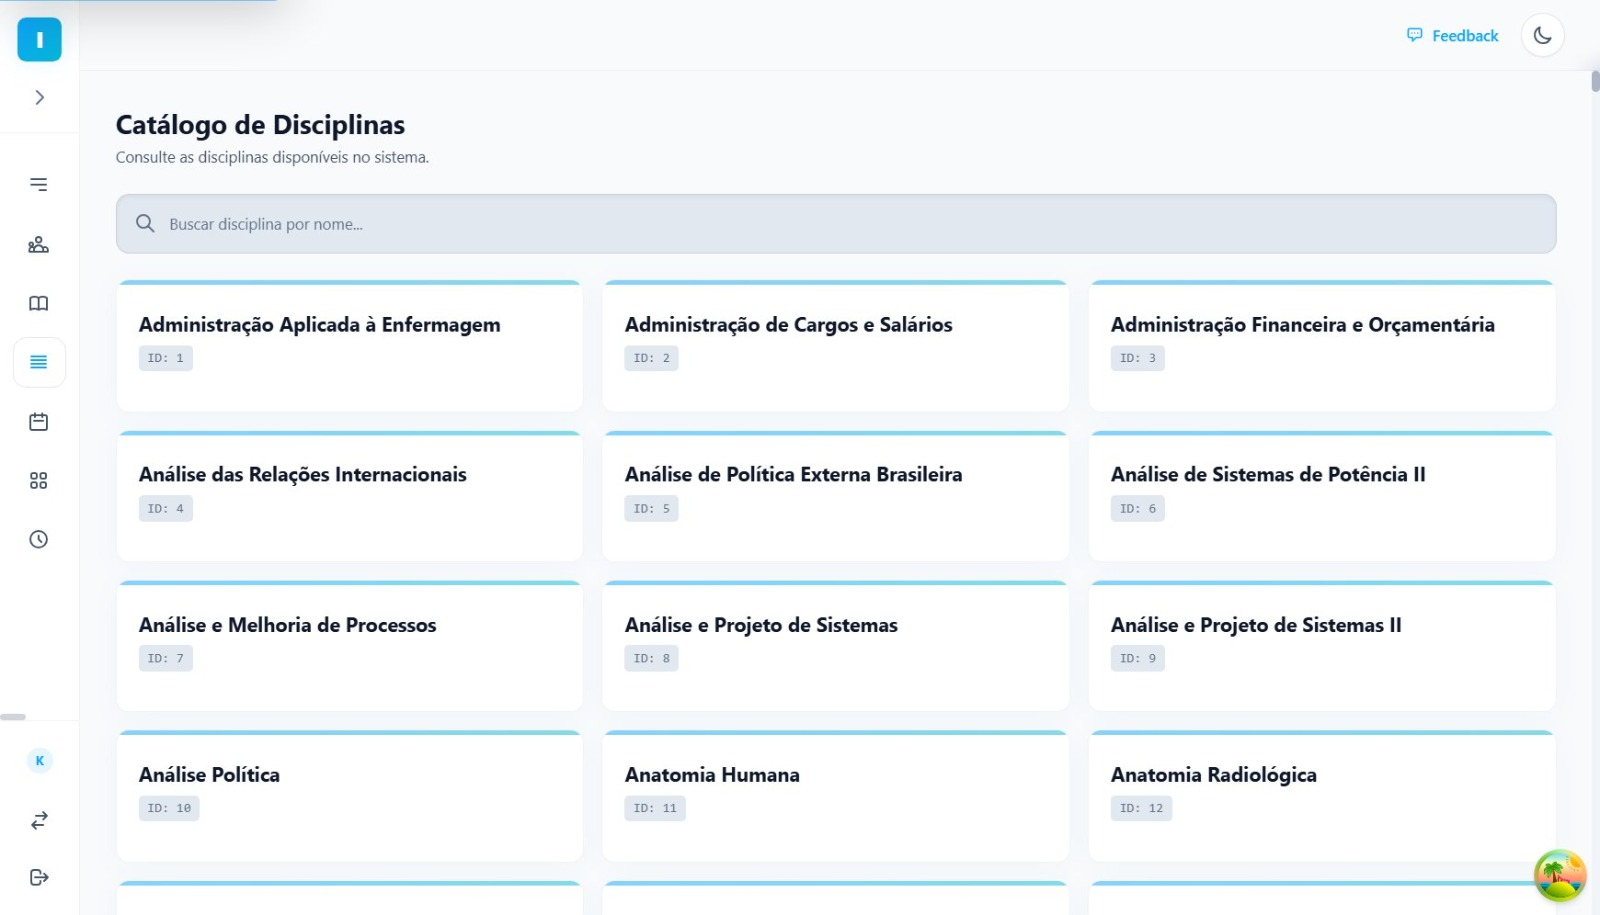
\includegraphics[width=\textwidth]{figuras/paginas/Figura_27_PG10.jpg}
\fonteautores
\end{figure}

No Catálogo de Disciplinas, o coordenador pode consultar todas as matérias que compõem o sistema. Uma barra de busca agiliza a localização de disciplinas específicas em meio aos diversos cartões que exibem o nome e ID de cada registro.

\begin{tabelainteracoes}{Interações do Catálogo de Disciplinas}{tab:interacoes-catalogo-disciplinas}
Pesquisar pelo nome da disciplina & O sistema filtra os cartões conforme o termo informado. & A pesquisa deve aceitar parte do nome e ignorar diferenças entre letras maiúsculas e minúsculas. \\
\hline
Limpar o campo de pesquisa & O sistema volta a apresentar todas as disciplinas disponíveis. & A listagem deve respeitar o contexto institucional e os filtros ativos. \\
\hline
Visualizar um cartão de disciplina & O sistema apresenta o nome e o identificador da matéria. & As informações são utilizadas posteriormente na composição de matrizes e áreas de atuação docente. \\
\hline
Clicar em uma disciplina & O sistema seleciona ou abre os detalhes do registro, quando essa ação estiver habilitada. & Alterações devem respeitar as permissões do perfil e preservar vínculos já utilizados em grades. \\
\hline
\end{tabelainteracoes}

% PG11.jpg
\begin{figure}[H]
\centering
\caption{Gerenciamento de Matriz da Turma}
\label{fig:PG11}
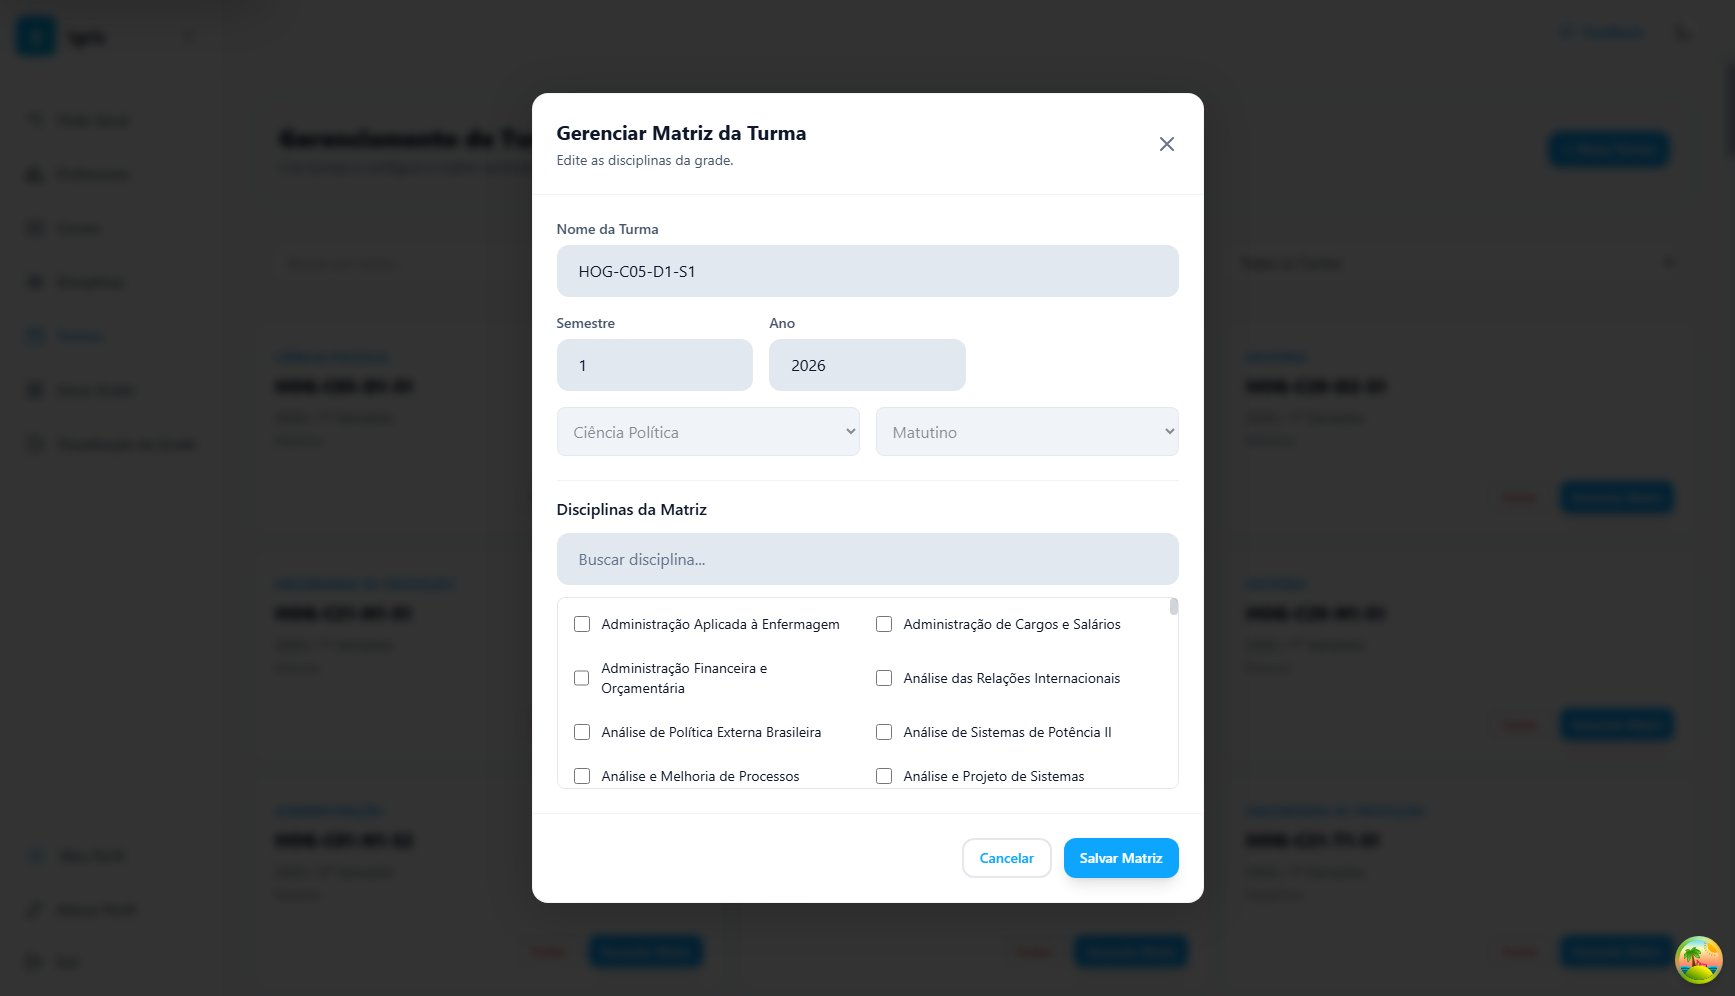
\includegraphics[width=\textwidth]{figuras/paginas/Figura_28_PG11.jpg}
\fonteautores
\end{figure}

Ao escolher gerenciar a matriz de uma turma, o sistema abre uma janela de edição. Nela, o coordenador visualiza os dados essenciais da turma em campos não editáveis e pode selecionar as disciplinas que farão parte da grade horária usando caixas de seleção, simplificando a montagem da matriz curricular.

\begin{tabelainteracoes}{Interações do Gerenciamento de Matriz da Turma}{tab:interacoes-matriz-turma}
Visualizar os dados da turma & O sistema apresenta nome, semestre, ano, curso e turno do registro selecionado. & Os campos contextuais permanecem bloqueados para evitar alterações acidentais durante a edição da matriz. \\
\hline
Pesquisar uma disciplina & O sistema filtra as opções disponíveis na lista da matriz. & A busca não modifica as seleções já realizadas. \\
\hline
Marcar ou desmarcar uma disciplina & O sistema inclui ou remove temporariamente a matéria da matriz da turma. & A mudança somente se torna definitiva após o salvamento. Disciplinas já alocadas podem exigir tratamento específico antes da remoção. \\
\hline
Clicar em ``Salvar Matriz'' & O sistema valida as seleções, atualiza os vínculos da matriz e fecha a janela. & Deve ser apresentada uma confirmação; falhas de persistência não podem descartar silenciosamente as escolhas. \\
\hline
Clicar em ``Cancelar'' ou fechar a janela & O sistema abandona as alterações não salvas e retorna à listagem de turmas. & A matriz anteriormente armazenada permanece inalterada. \\
\hline
\end{tabelainteracoes}

% PG13.jpg
\begin{figure}[H]
\centering
\caption{Criação de Nova Turma}
\label{fig:PG13}
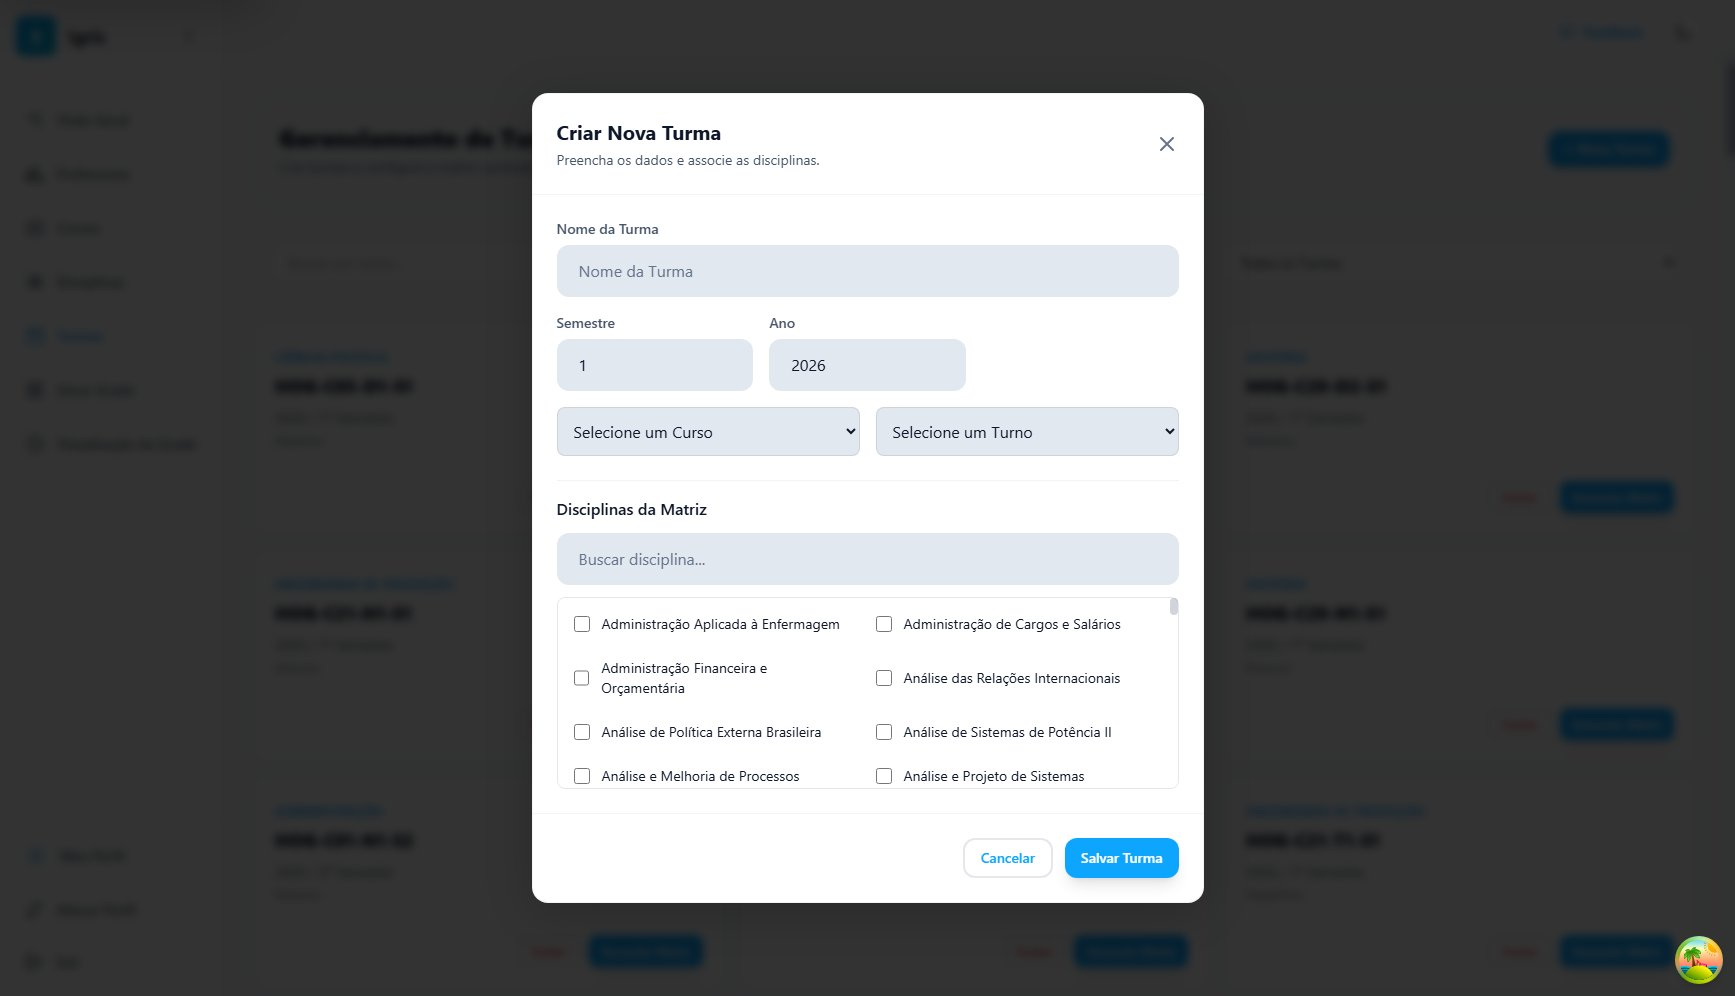
\includegraphics[width=\textwidth]{figuras/paginas/Figura_29_PG13.jpg}
\fonteautores
\end{figure}

A tela "Criar Nova Turma" funciona como um formulário em formato modal onde o usuário insere o nome, período, curso e turno da turma a ser criada. Simultaneamente, o usuário pode associar as disciplinas da matriz utilizando uma lista com caixas de seleção.

\begin{tabelainteracoes}{Interações da Criação de Nova Turma}{tab:interacoes-criacao-turma}
Informar o nome da turma & O sistema registra o nome ou código que identificará o novo grupo acadêmico. & O campo é obrigatório e deve evitar duplicidade dentro do mesmo período e contexto institucional. \\
\hline
Informar semestre e ano & O sistema define o período letivo ao qual a turma pertencerá. & Os valores devem representar um período válido; o ano deve ser numérico e o semestre deve estar entre as opções permitidas. \\
\hline
Selecionar curso e turno & O sistema vincula a turma ao curso e ao turno escolhidos. & Ambos os campos são obrigatórios e devem conter somente opções autorizadas para a coordenação ativa. \\
\hline
Pesquisar, marcar ou desmarcar disciplinas & O sistema monta temporariamente a matriz inicial da nova turma. & As seleções devem pertencer ao curso escolhido e somente serão persistidas com a criação da turma. \\
\hline
Clicar em ``Salvar Turma'' & O sistema valida os dados, cria a turma e salva os vínculos da matriz. & Em caso de sucesso, a janela é fechada e a listagem atualizada; dados inválidos devem ser destacados sem criar registros parciais. \\
\hline
Clicar em ``Cancelar'' ou fechar a janela & O sistema abandona o preenchimento e retorna ao gerenciamento de turmas. & Nenhuma turma ou matriz deve ser criada. \\
\hline
\end{tabelainteracoes}

% PG14.jpg
\begin{figure}[H]
\centering
\caption{Motor de Alocação - Configuração Inicial}
\label{fig:PG14}
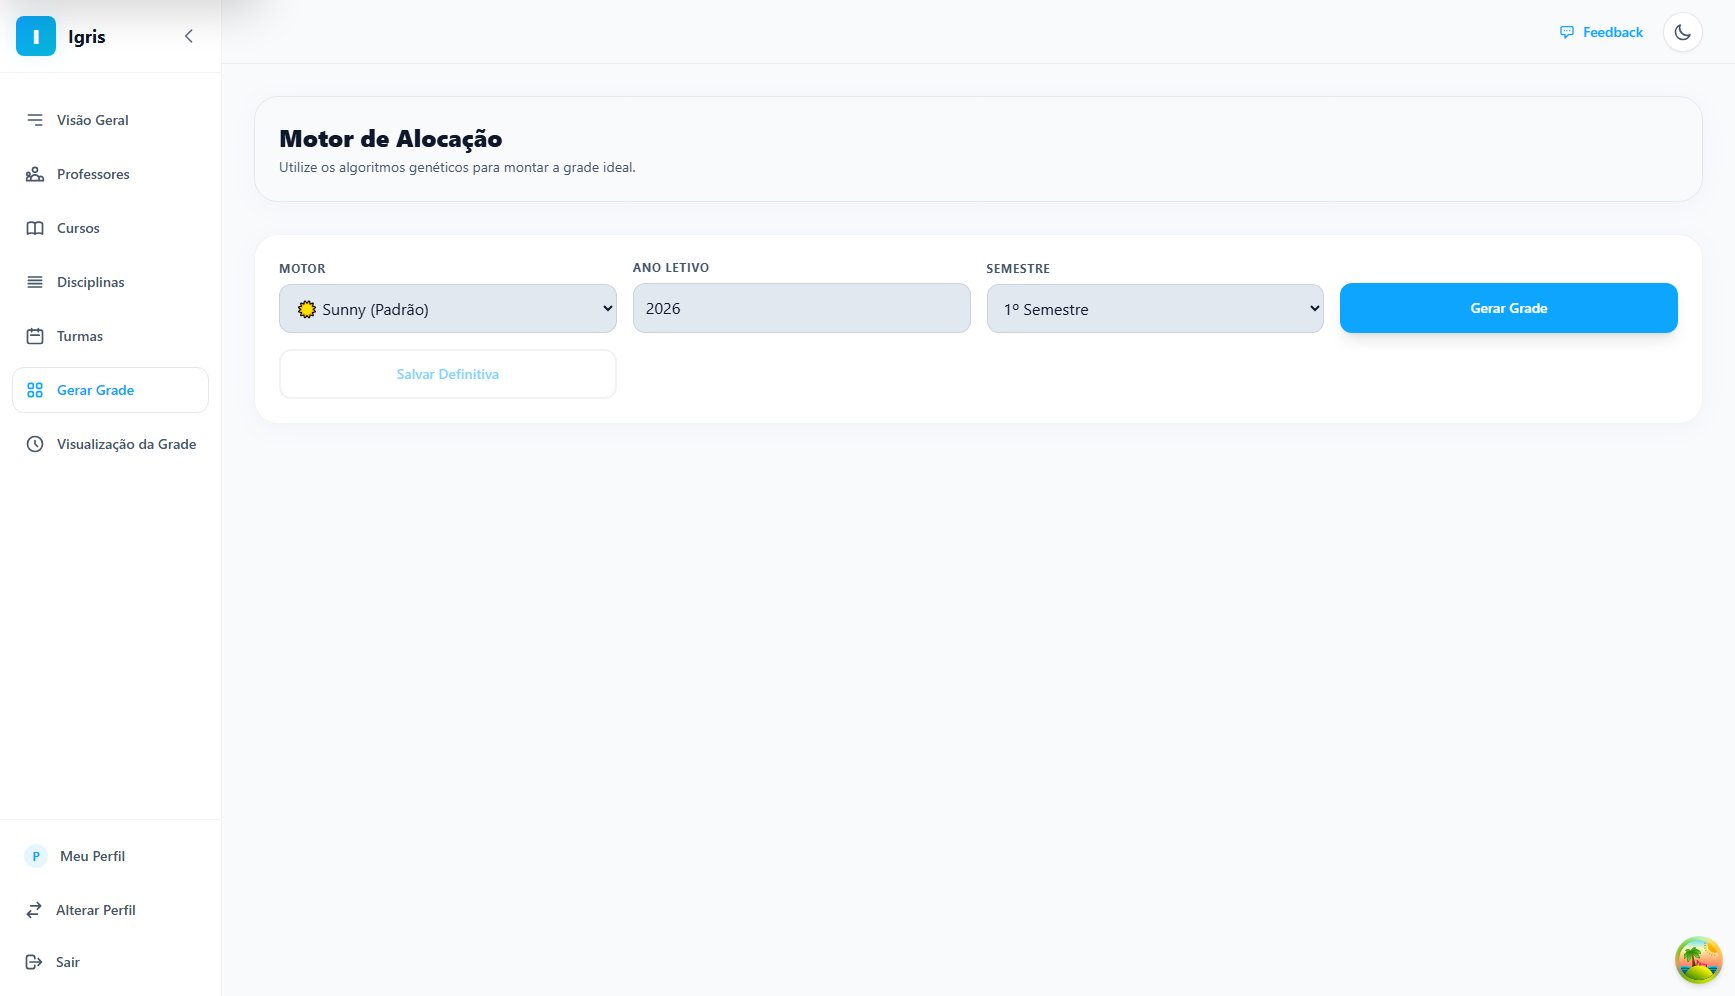
\includegraphics[width=\textwidth]{figuras/paginas/Figura_30_PG14.jpg}
\fonteautores
\end{figure}

A tela do Motor de Alocação é onde a geração da grade horária ocorre. O usuário seleciona o modelo de algoritmo desejado, como o Sunny (Padrão), além de especificar o ano letivo e o semestre, iniciando então o processamento com o botão "Gerar Grade".

\begin{tabelainteracoes}{Interações do Motor de Alocação -- Configuração Inicial}{tab:interacoes-motor-configuracao}
Selecionar o modelo de algoritmo & O sistema define o motor que processará a geração da grade. & Somente modelos disponíveis e configurados, como Sunny ou Morpheus, devem ser apresentados. \\
\hline
Informar o ano letivo & O sistema utiliza o ano para identificar turmas, matrizes e disponibilidades aplicáveis. & O campo é obrigatório e deve aceitar apenas um ano válido. \\
\hline
Selecionar o semestre & O sistema restringe a geração ao período letivo escolhido. & Deve ser selecionada uma das opções de semestre cadastradas. \\
\hline
Clicar em ``Gerar Grade'' & O sistema valida os dados, envia o problema ao motor selecionado e apresenta o estado de processamento. & O botão deve evitar solicitações duplicadas enquanto a execução estiver em andamento. \\
\hline
Tentar gerar sem dados acadêmicos suficientes & O sistema interrompe a operação e informa quais cadastros ou disponibilidades precisam ser completados. & Turmas sem matriz, disciplinas sem professor apto ou ausência de disponibilidade podem impedir ou comprometer a geração. \\
\hline
\end{tabelainteracoes}

% PG15.jpg
\begin{figure}[H]
\centering
\caption{Resultados do Motor de Alocação}
\label{fig:PG15}
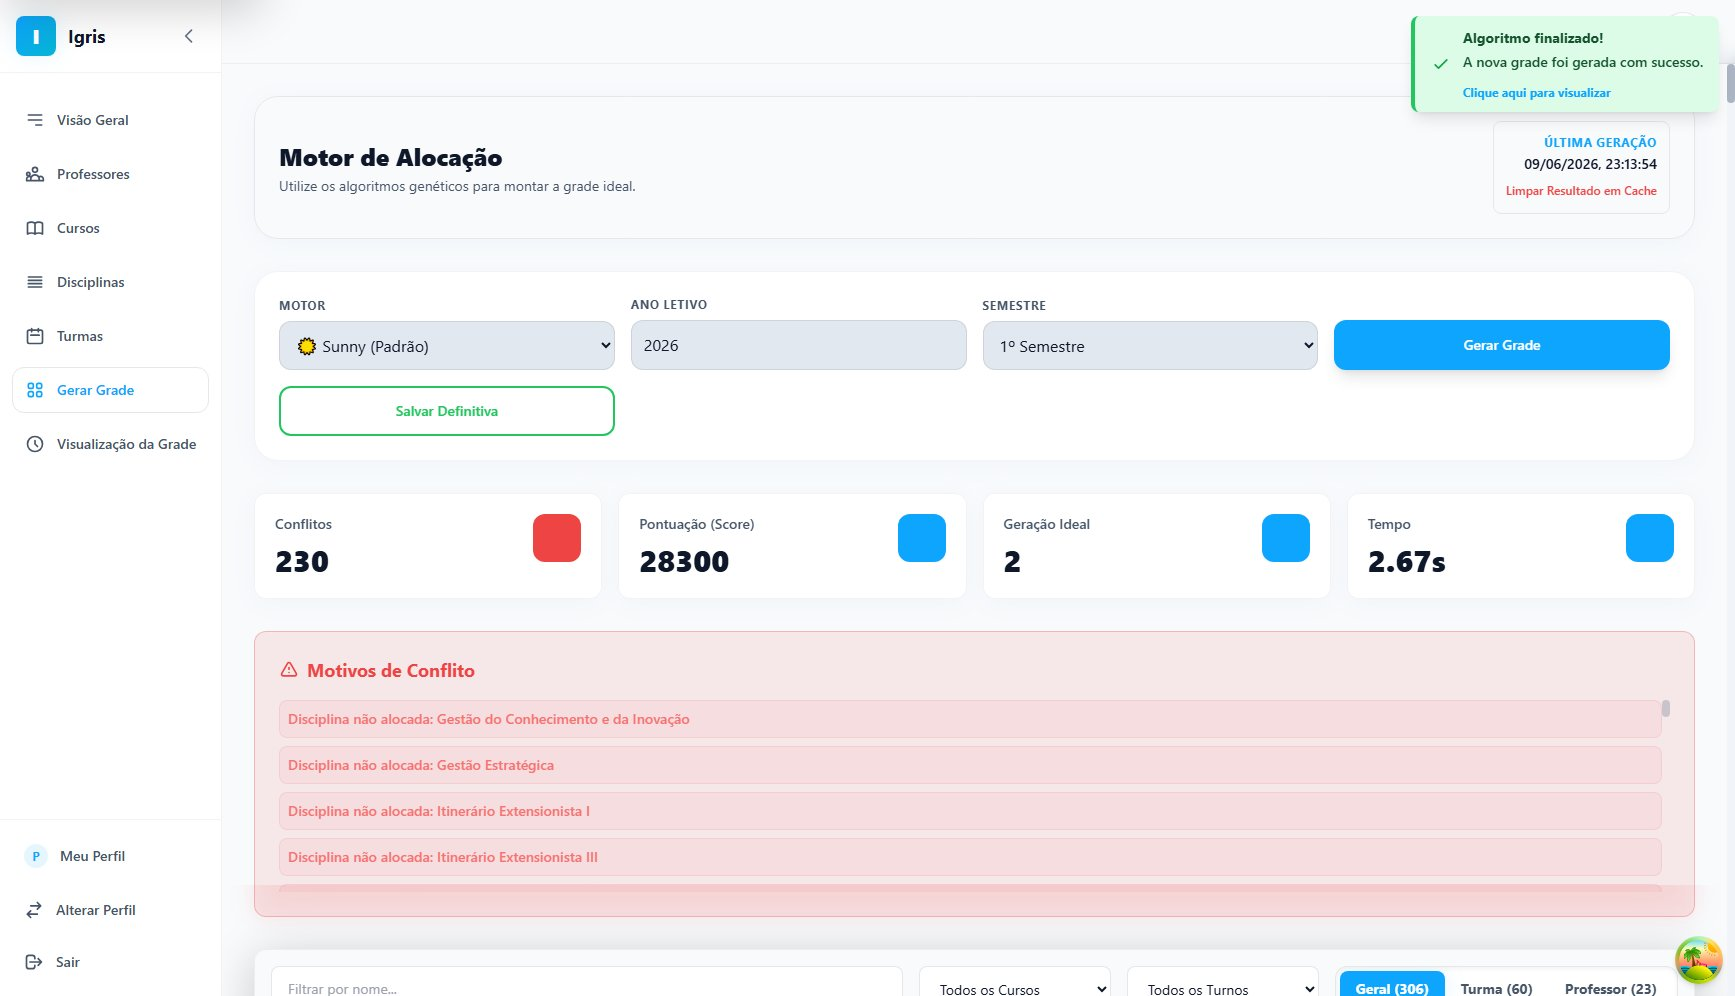
\includegraphics[width=\textwidth]{figuras/paginas/Figura_31_PG15.jpg}
\fonteautores
\end{figure}

Após o término da execução, o Motor de Alocação apresenta métricas valiosas como o número de conflitos restantes, a pontuação (score) obtida, a geração ideal e o tempo de execução do algoritmo. Uma área de alerta destaca as disciplinas que não puderam ser alocadas, indicando os gargalos.

\begin{tabelainteracoes}{Interações dos Resultados do Motor de Alocação}{tab:interacoes-resultados-motor}
Aguardar a conclusão do algoritmo & O sistema atualiza a tela com o resultado, as métricas de execução e uma notificação de término. & A interface deve distinguir claramente processamento, sucesso e falha. \\
\hline
Consultar conflitos, pontuação, geração e tempo & O sistema apresenta os indicadores produzidos pelo motor de alocação. & Os valores permitem avaliar a qualidade da solução e comparar diferentes configurações. \\
\hline
Consultar ``Motivos de Conflito'' & O sistema lista disciplinas e restrições que impediram determinadas alocações. & Os itens devem fornecer informação suficiente para que o gestor corrija cadastros, matrizes ou disponibilidades. \\
\hline
Clicar em ``Salvar Definitivo'' & O sistema solicita confirmação e persiste a grade e suas alocações. & Uma solução com conflitos deve exigir ciência do usuário ou ser bloqueada conforme a regra institucional. \\
\hline
Clicar em ``Gerar Novamente'' & O sistema inicia uma nova execução utilizando os parâmetros selecionados. & O resultado anterior não deve substituir uma grade já salva sem confirmação. \\
\hline
Ocorrer falha durante o processamento & O sistema informa que a geração não foi concluída e mantém os parâmetros para uma nova tentativa. & Nenhuma grade incompleta deve ser registrada como definitiva. \\
\hline
\end{tabelainteracoes}

% PG16.jpg
\begin{figure}[H]
\centering
\caption{Visualização Geral da Grade com Alertas}
\label{fig:PG16}
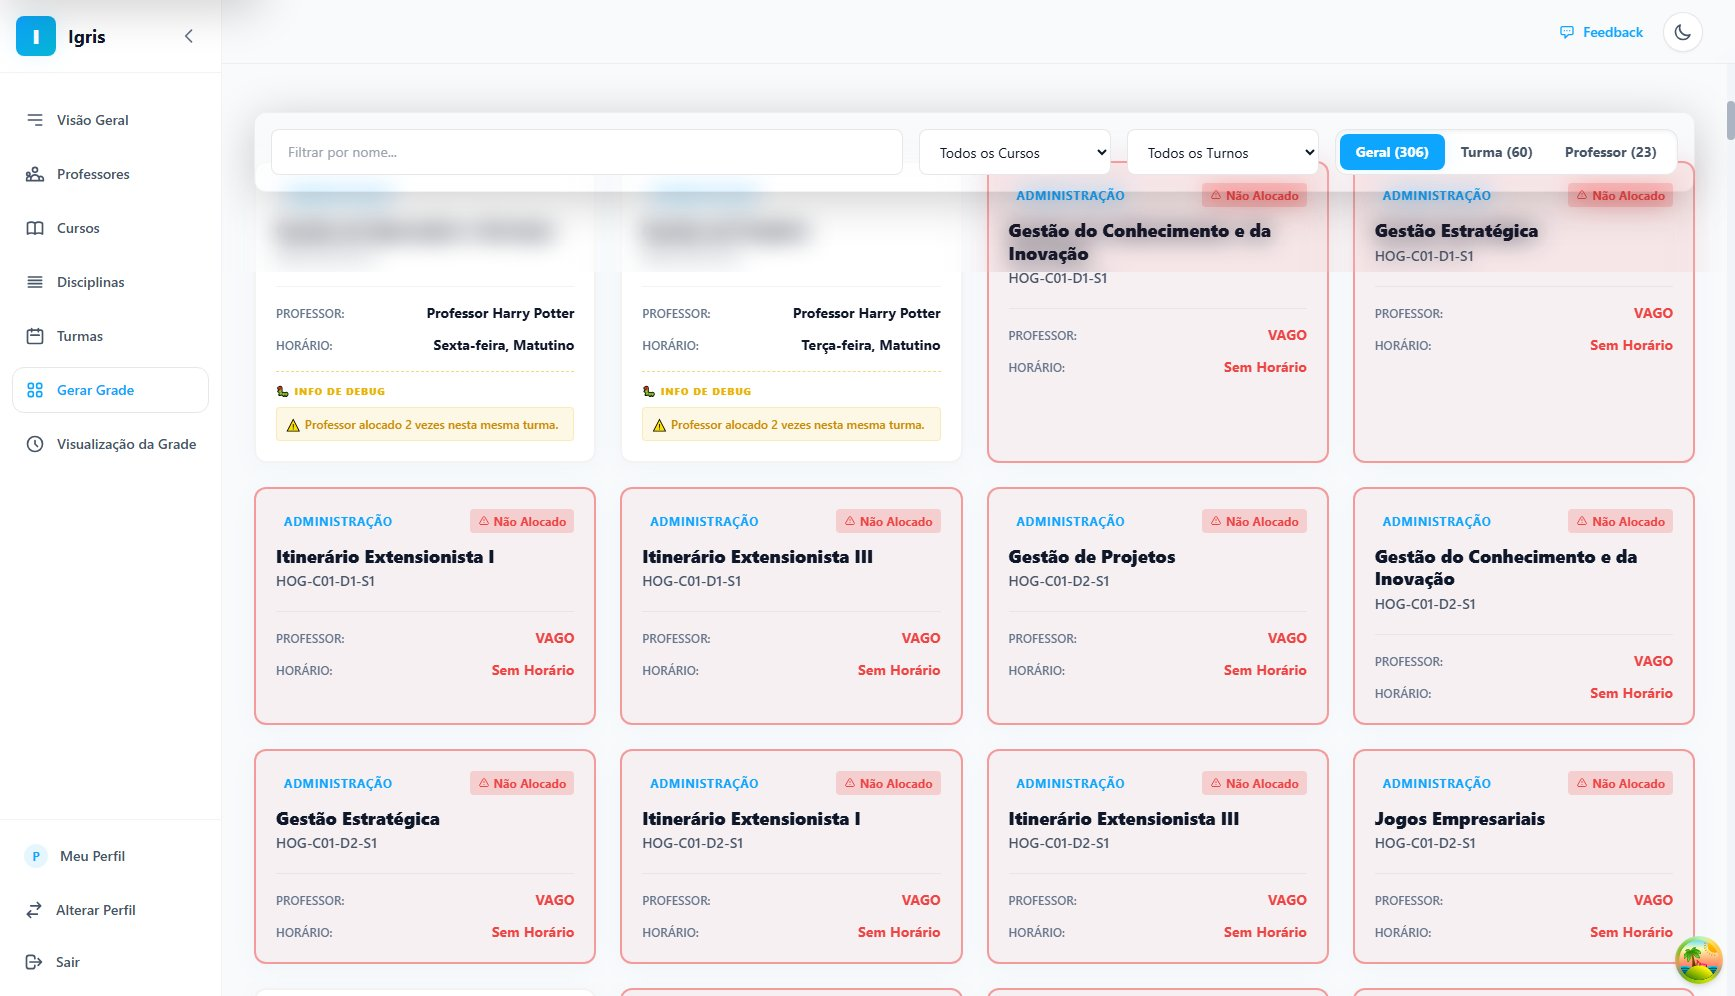
\includegraphics[width=\textwidth]{figuras/paginas/Figura_32_PG16.jpg}
\fonteautores
\end{figure}

A interface de Visualização da Grade possibilita a inspeção das aulas alocadas de forma generalizada. Ela apresenta as interações entre disciplinas, turmas e professores, destacando claramente em vermelho situações onde uma disciplina permanece "Não Alocada" ou quando faltam horários.

\begin{tabelainteracoes}{Interações da Visualização Geral da Grade com Alertas}{tab:interacoes-grade-alertas}
Pesquisar uma turma, disciplina ou professor & O sistema filtra os cartões da grade conforme o termo informado. & A busca deve abranger os dados relevantes exibidos em cada alocação. \\
\hline
Selecionar curso ou turno & O sistema exibe somente as alocações compatíveis com os filtros escolhidos. & Os filtros podem ser combinados e não alteram a grade armazenada. \\
\hline
Alternar entre as visões Geral, Turmas e Professores & O sistema reorganiza os mesmos dados conforme a perspectiva escolhida. & A quantidade indicada em cada aba deve refletir os registros disponíveis. \\
\hline
Visualizar um cartão destacado em vermelho & O sistema apresenta a disciplina como não alocada ou sem horário definido. & O alerta indica pendência que deve ser tratada antes da validação definitiva da grade. \\
\hline
Consultar o motivo de uma pendência & O sistema apresenta as informações disponíveis sobre professor, turma, horário ou restrição conflitante. & A ausência de professor apto ou de disponibilidade deve ser explicitada quando identificável. \\
\hline
\end{tabelainteracoes}

% PG17.jpg
\begin{figure}[H]
\centering
\caption{Grade Horária - Visão por Turma (Cartões)}
\label{fig:PG17}
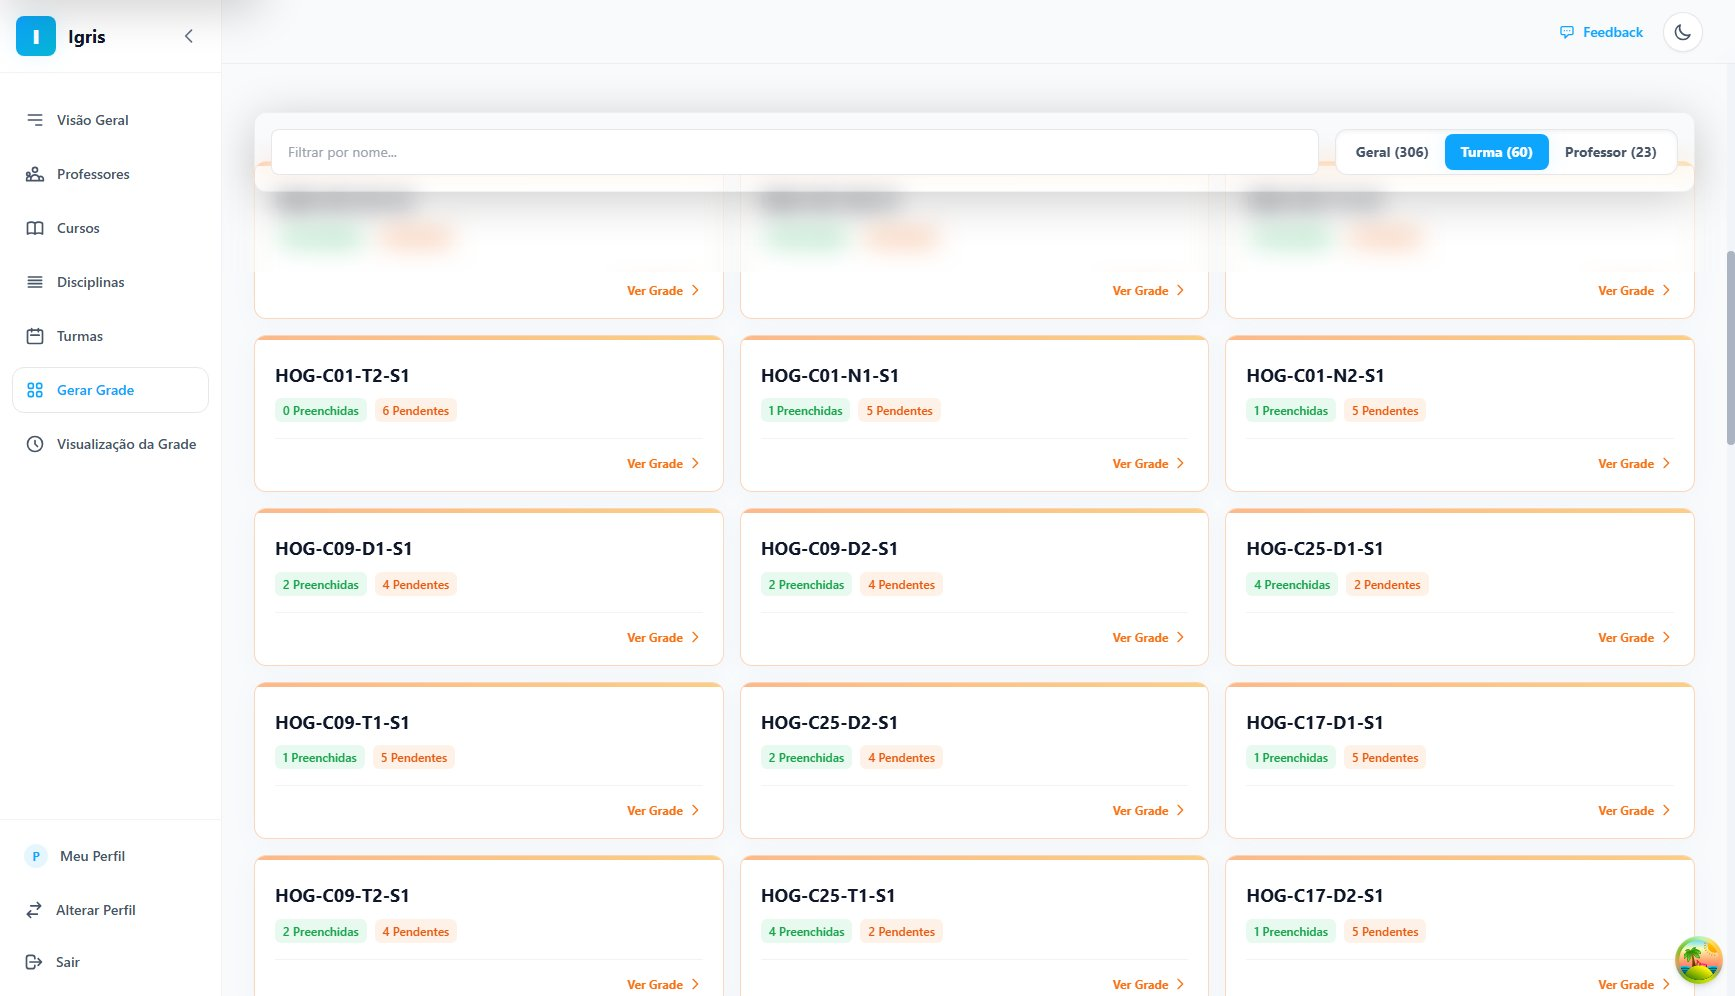
\includegraphics[width=\textwidth]{figuras/paginas/Figura_33_PG17.jpg}
\fonteautores
\end{figure}

A Grade Horária pode ser vista sob a perspectiva das turmas. Em formato de cartões, o coordenador pode avaliar o status de cada turma (ex: 3 Preenchidas, 1 Pendentes), facilitando a identificação das classes que precisam de intervenções.

\begin{tabelainteracoes}{Interações da Grade Horária -- Visão por Turma}{tab:interacoes-grade-por-turma}
Selecionar a aba ``Turmas'' & O sistema agrupa as alocações em cartões correspondentes a cada turma. & Cada cartão deve resumir a quantidade de horários preenchidos e pendentes. \\
\hline
Pesquisar uma turma & O sistema filtra os cartões pelo nome ou identificador informado. & A pesquisa não modifica as alocações existentes. \\
\hline
Clicar em ``Ver Grade'' & O sistema abre a matriz semanal detalhada da turma selecionada. & O detalhamento deve apresentar somente aulas e pendências relacionadas à turma acionada. \\
\hline
Visualizar o indicador de pendências & O sistema destaca a quantidade de componentes ainda não alocados. & A cor e o texto do indicador devem permitir diferenciar uma grade completa de uma incompleta. \\
\hline
Não existir grade para o período & O sistema informa que não há dados disponíveis para exibição. & O usuário pode ser orientado a gerar ou selecionar outra grade. \\
\hline
\end{tabelainteracoes}

% PG18.jpg
\begin{figure}[H]
\centering
\caption{Detalhamento da Matriz Semanal de uma Turma}
\label{fig:PG18}
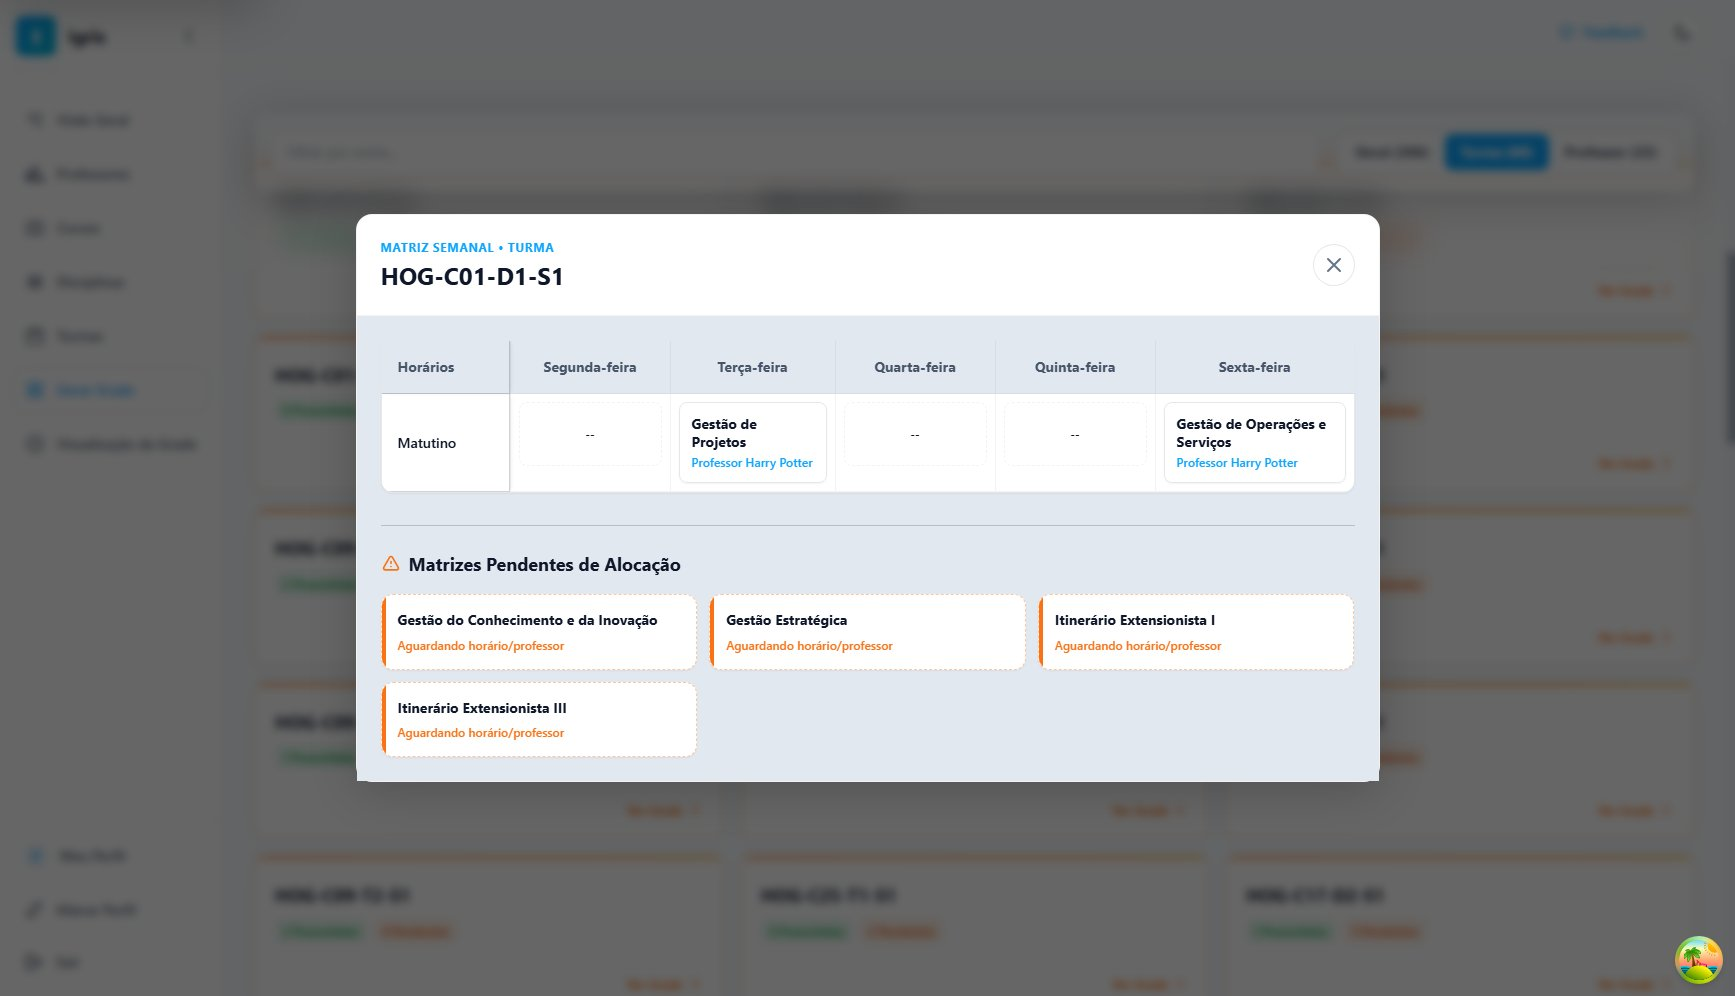
\includegraphics[width=\textwidth]{figuras/paginas/Figura_34_PG18.jpg}
\fonteautores
\end{figure}

Ao clicar em uma turma, um detalhamento semanal é exibido. A janela cruza os dias da semana e turnos mostrando as disciplinas e seus respectivos professores alocados para aquela turma, facilitando a visualização.

\begin{tabelainteracoes}{Interações do Detalhamento Semanal de uma Turma}{tab:interacoes-detalhamento-turma}
Abrir o detalhamento de uma turma & O sistema apresenta uma matriz com dias da semana, turnos, disciplinas e professores alocados. & O cabeçalho deve identificar claramente a turma consultada. \\
\hline
Consultar uma célula preenchida & O sistema exibe a disciplina e o professor designados para aquele dia e turno. & Uma mesma turma não pode possuir duas aulas simultâneas no mesmo intervalo. \\
\hline
Consultar uma célula vazia & O sistema indica que não há aula alocada naquele período. & A célula vazia pode representar horário livre, conforme a matriz e a carga horária previstas. \\
\hline
Consultar ``Matrizes Pendentes de Alocação'' & O sistema lista as disciplinas da turma que ainda não receberam horário ou professor. & As pendências devem permanecer visíveis até que uma nova geração ou correção seja realizada. \\
\hline
Clicar no ícone de fechar & O sistema encerra o detalhamento e retorna à visão por turmas. & Os dados são apenas consultados; fechar a janela não altera a grade. \\
\hline
\end{tabelainteracoes}

% PG19.jpg
\begin{figure}[H]
\centering
\caption{Grade Horária - Visão por Professor}
\label{fig:PG19}
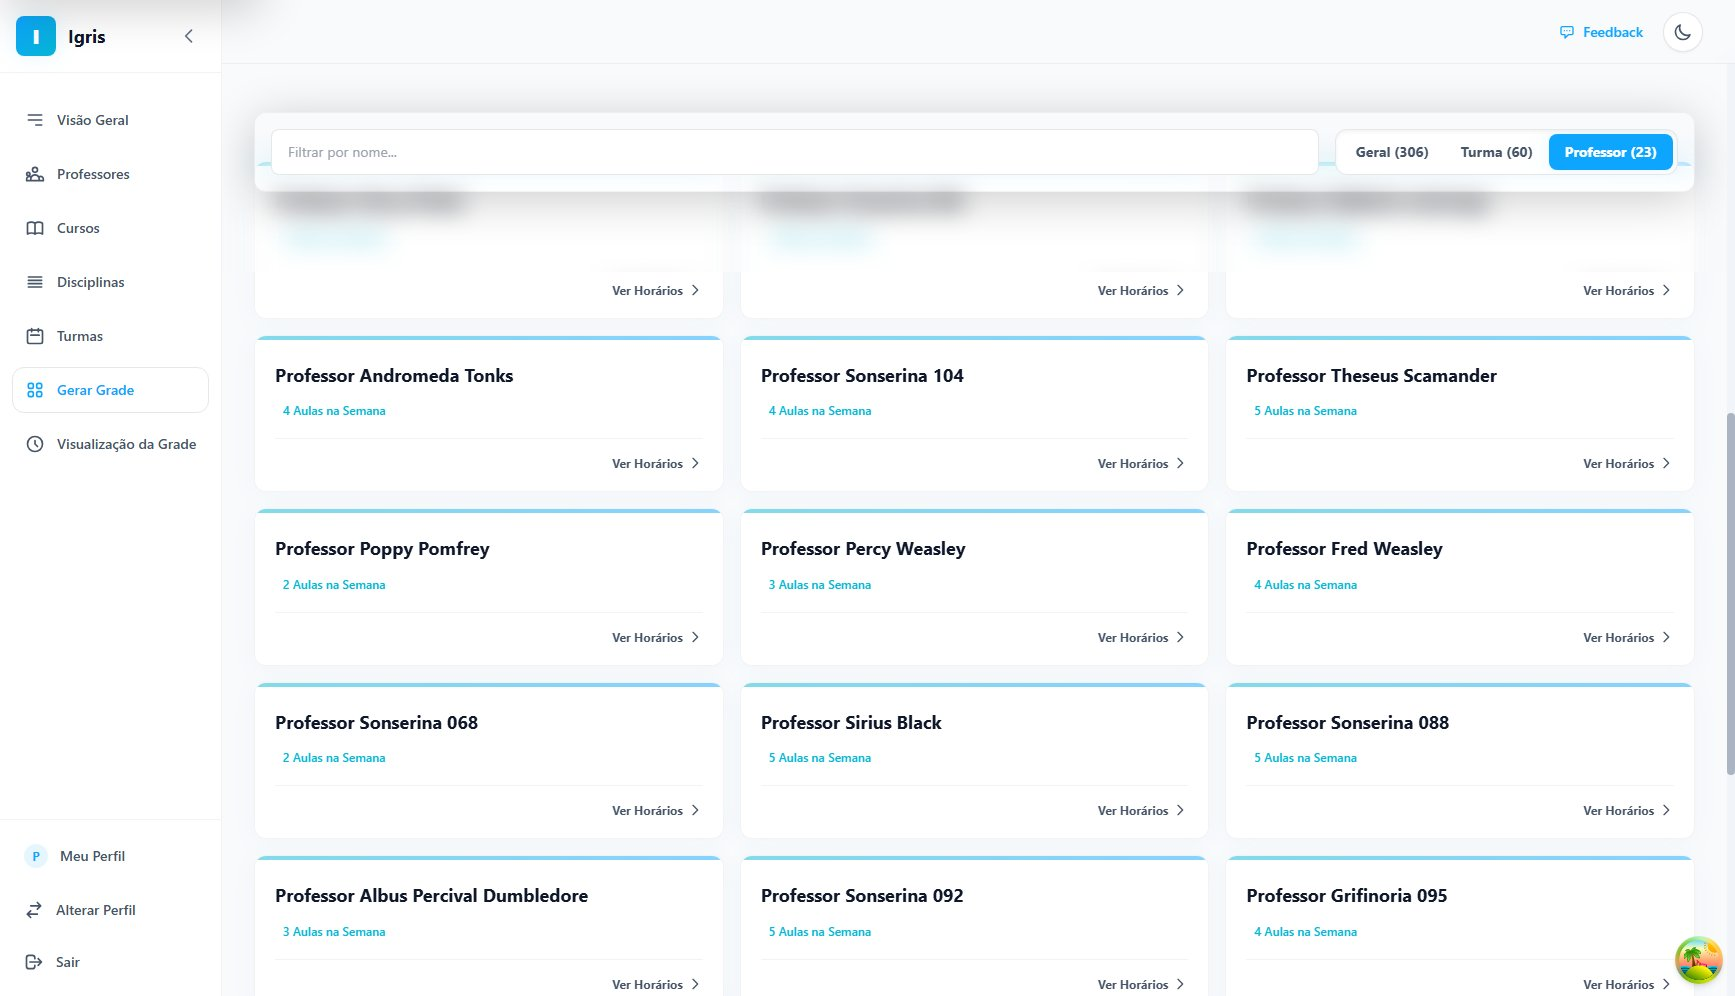
\includegraphics[width=\textwidth]{figuras/paginas/Figura_35_PG19.jpg}
\fonteautores
\end{figure}

A visão por professor exibe o total de aulas designadas na semana para cada docente. Os cartões fornecem um panorama rápido da carga horária que foi alocada a eles, essencial para a validação da adequação aos contratos de trabalho.

\begin{tabelainteracoes}{Interações da Grade Horária -- Visão por Professor}{tab:interacoes-grade-por-professor}
Selecionar a aba ``Professores'' & O sistema agrupa as aulas por docente e apresenta um cartão para cada professor. & A contagem exibida deve considerar somente a grade e o período selecionados. \\
\hline
Pesquisar um professor & O sistema filtra os cartões conforme o nome informado. & Quando não houver resultado, deve ser exibido um estado de lista vazia. \\
\hline
Consultar a quantidade de aulas da semana & O sistema mostra a carga semanal atribuída ao professor. & O indicador auxilia a identificar subalocação ou excesso de carga, mas deve ser comparado às regras contratuais cadastradas. \\
\hline
Clicar em ``Ver Horários'' & O sistema abre a matriz semanal individual do professor selecionado. & A janela deve apresentar apenas as alocações vinculadas ao docente acionado. \\
\hline
Identificar sobreposição de aulas & O sistema destaca ou informa o conflito de horários do professor. & Um docente não pode ser alocado simultaneamente em turmas diferentes. \\
\hline
\end{tabelainteracoes}

% PG20.jpg
\begin{figure}[H]
\centering
\caption{Detalhamento da Matriz Semanal de um Professor}
\label{fig:PG20}
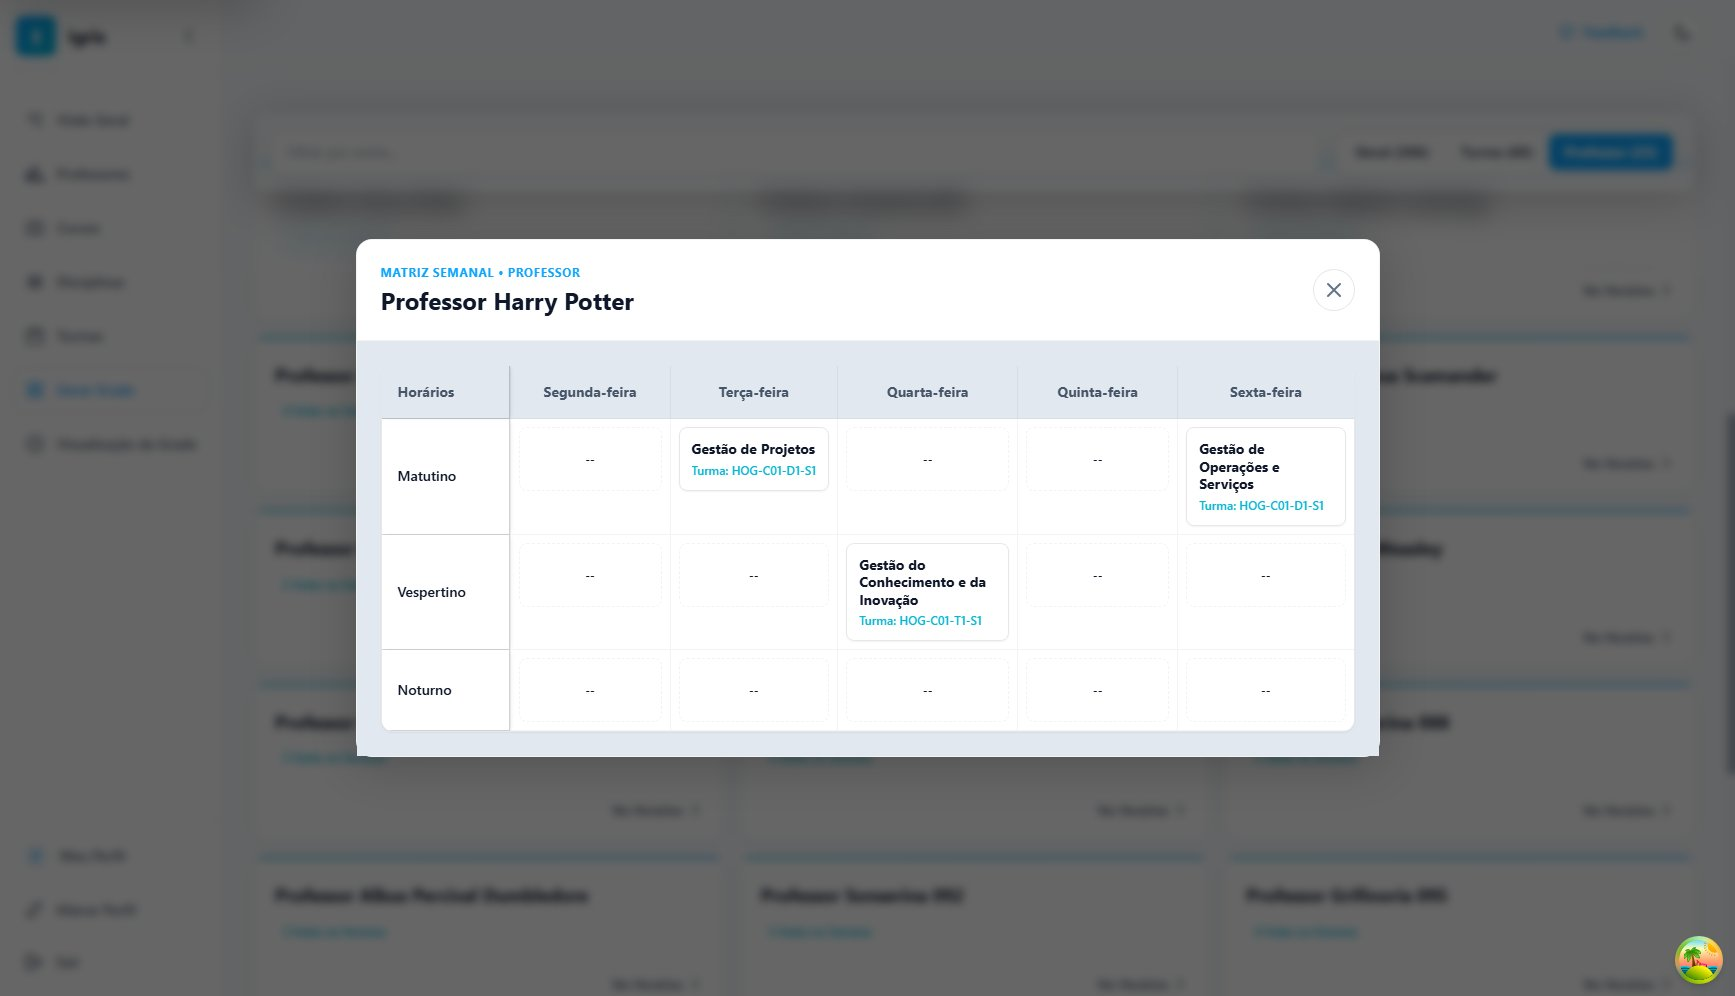
\includegraphics[width=\textwidth]{figuras/paginas/Figura_36_PG20.jpg}
\fonteautores
\end{figure}

Clicar sobre o cartão de um professor exibe a sua matriz semanal. O sistema apresenta em quais dias e horários o professor estará lecionando, junto com as disciplinas e turmas para as quais ele foi designado.

\begin{tabelainteracoes}{Interações do Detalhamento Semanal de um Professor}{tab:interacoes-detalhamento-professor}
Abrir os horários de um professor & O sistema apresenta a matriz semanal individual, organizada por dias e turnos. & O cabeçalho deve indicar o nome do docente consultado. \\
\hline
Consultar uma aula alocada & O sistema exibe a disciplina e a turma correspondentes ao horário. & A alocação deve respeitar a disponibilidade e as áreas de atuação cadastradas para o professor. \\
\hline
Consultar um período sem aula & O sistema mantém a célula vazia ou a identifica como livre. & A ausência de aula não significa necessariamente disponibilidade, pois pode existir uma restrição cadastrada. \\
\hline
Detectar duas aulas no mesmo horário & O sistema deve sinalizar a inconsistência para correção. & Sobreposições representam conflito impeditivo na grade do docente. \\
\hline
Clicar no ícone de fechar & O sistema fecha a matriz individual e retorna à visão por professores. & A consulta não modifica as alocações. \\
\hline
\end{tabelainteracoes}

% PG21.jpg
\begin{figure}[H]
\centering
\caption{Acompanhamento Geral das Pendências}
\label{fig:PG21}
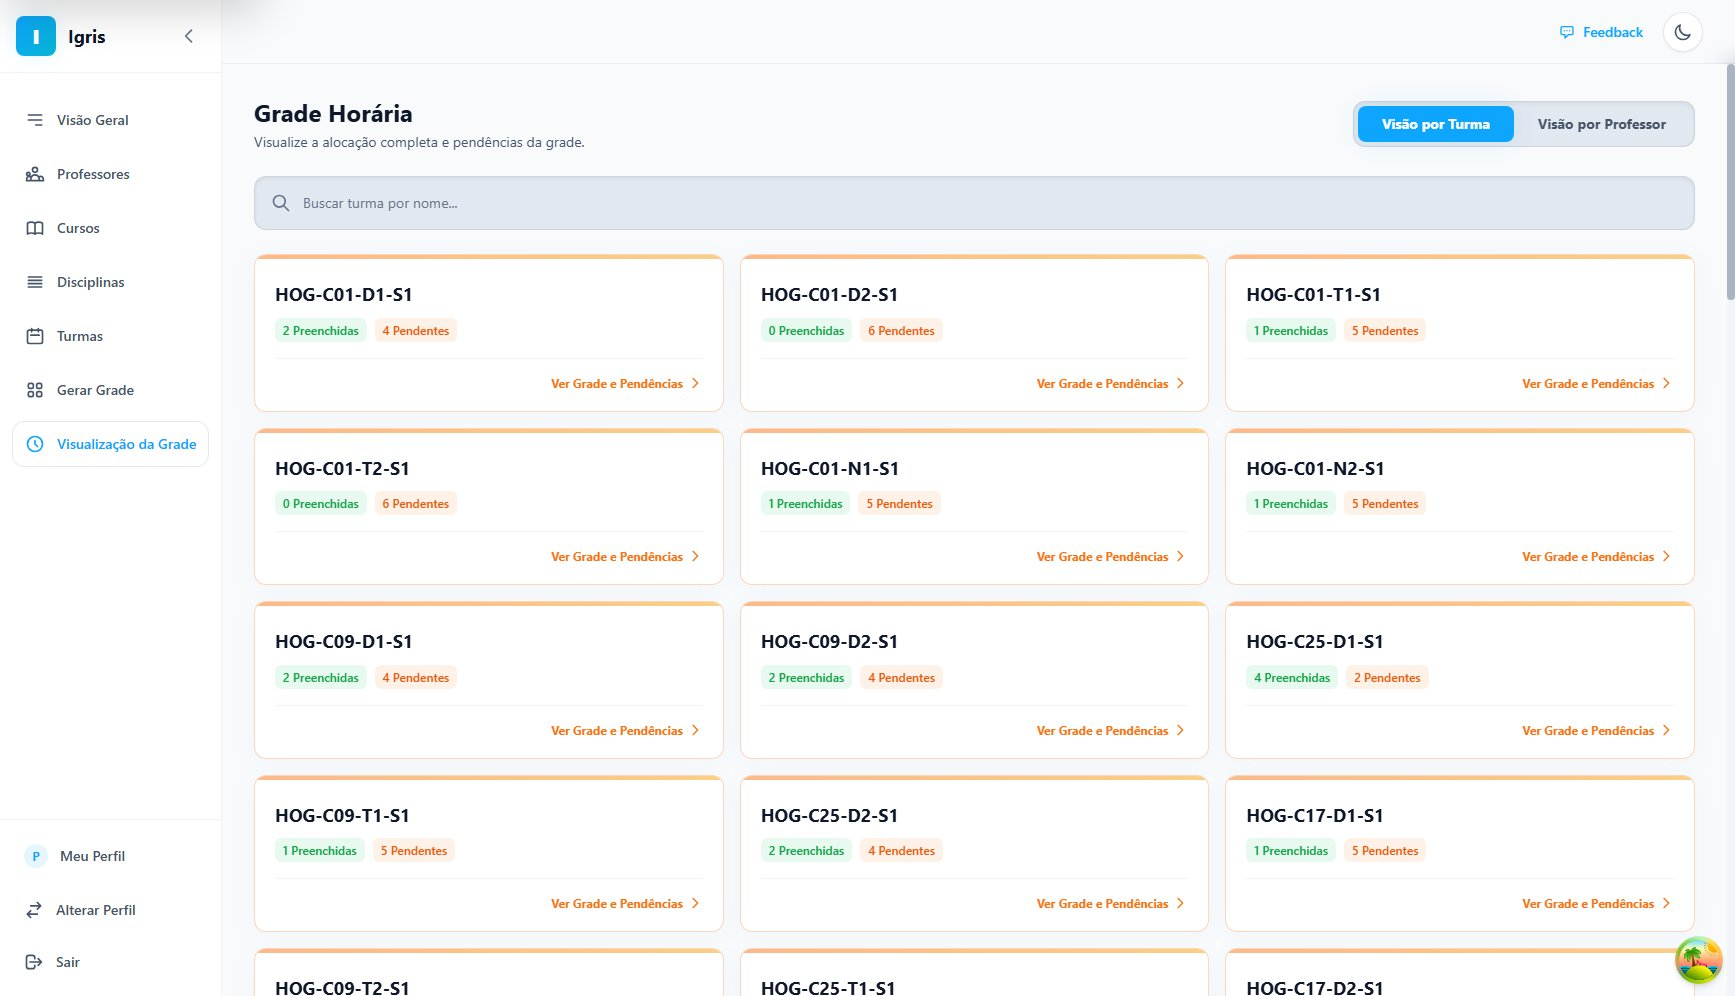
\includegraphics[width=\textwidth]{figuras/paginas/Figura_37_PG21.jpg}
\fonteautores
\end{figure}

A visão por turma na Grade Horária reforça a visualização em cartões, permitindo uma alternância ágil entre a visão de turmas e de professores, sempre indicando em destaque onde existem pendências e horários preenchidos.

\begin{tabelainteracoes}{Interações do Acompanhamento Geral das Pendências}{tab:interacoes-acompanhamento-pendencias}
Alternar entre ``Visão por Turma'' e ``Visão por Professor'' & O sistema reorganiza a grade pela perspectiva escolhida. & A alternância não executa nova geração nem modifica os dados salvos. \\
\hline
Pesquisar pelo nome & O sistema filtra a relação de turmas ou professores da visão ativa. & O campo deve ser limpo ou reaplicado corretamente ao trocar de visão. \\
\hline
Consultar indicadores de preenchimento e pendência & O sistema apresenta um resumo quantitativo em cada cartão. & Os valores devem ser atualizados sempre que uma nova grade for salva. \\
\hline
Clicar no detalhamento de um cartão & O sistema abre a matriz semanal e, quando aplicável, a lista de pendências. & O usuário deve conseguir identificar o item que exige intervenção. \\
\hline
Não haver pendências & O sistema apresenta os cartões como completos, sem alertas de alocação. & A ausência de pendências não dispensa a validação de carga e conflitos pelo gestor. \\
\hline
\end{tabelainteracoes}

% PG23.jpg
\begin{figure}[H]
\centering
\caption{Grade Horária - Detalhamento de Turma e Pendências}
\label{fig:PG23}
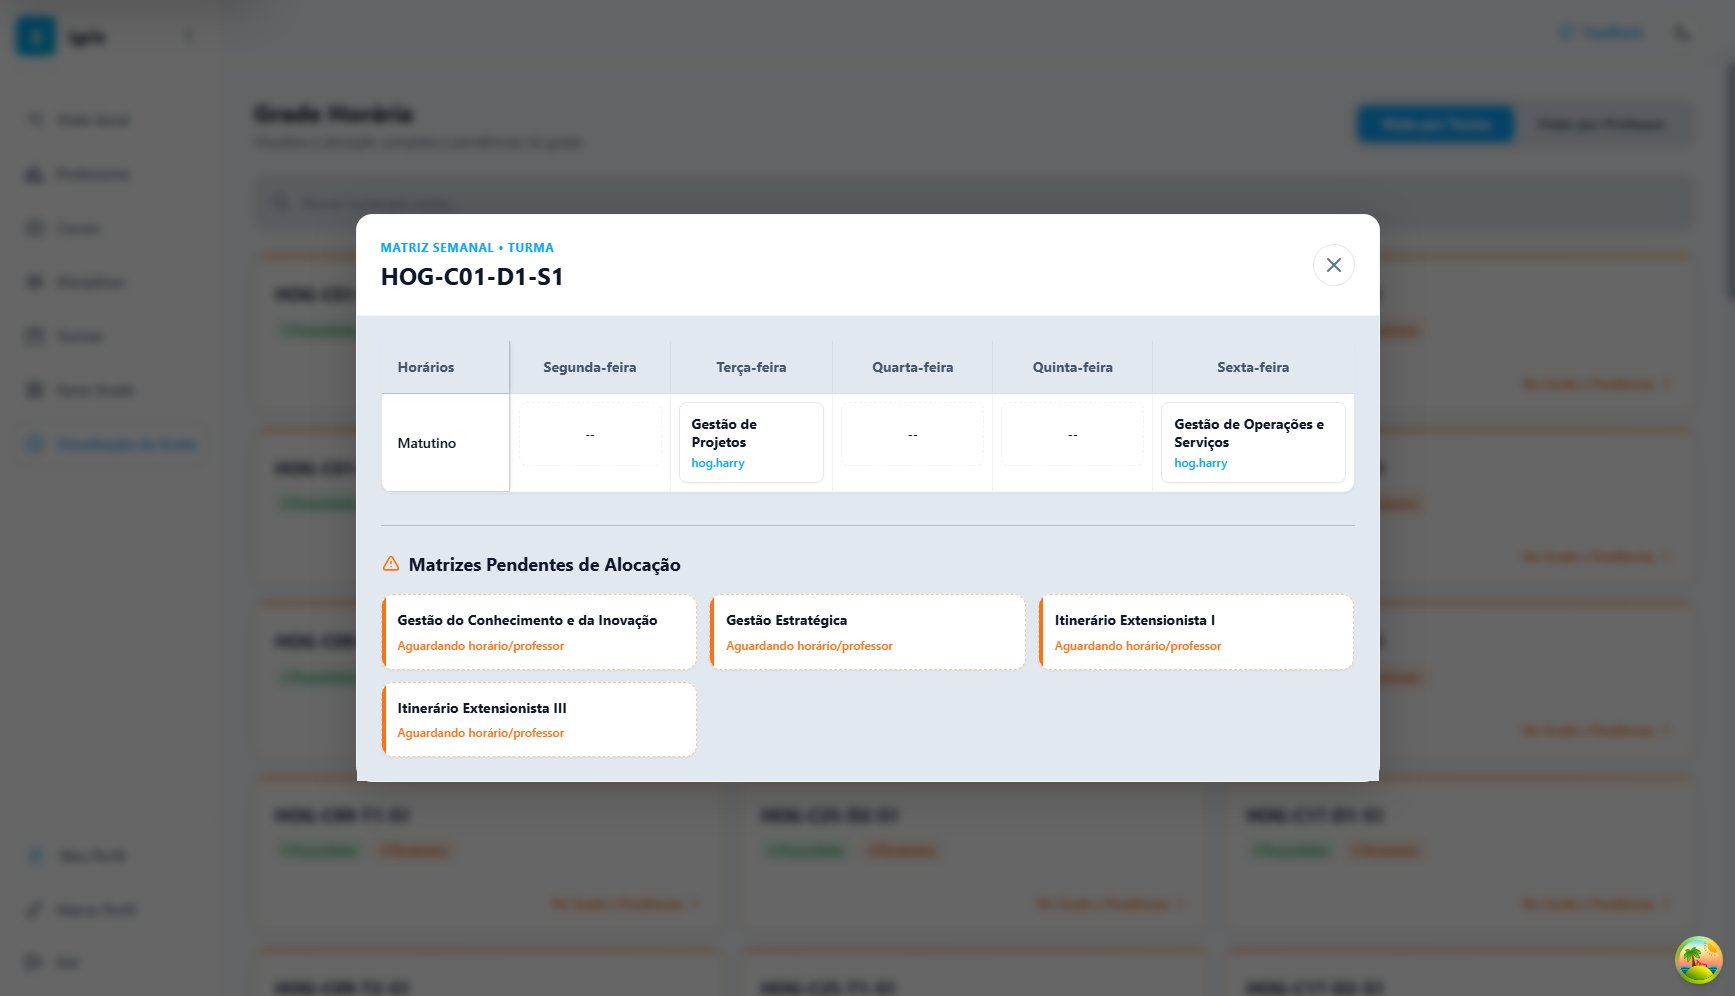
\includegraphics[width=\textwidth]{figuras/paginas/Figura_38_PG23.jpg}
\fonteautores
\end{figure}

A tela apresenta o detalhamento da grade semanal de uma turma selecionada. A matriz relaciona os dias da semana aos turnos e identifica as disciplinas, os professores e as turmas presentes em cada horário. Na parte inferior, a interface também reúne as disciplinas da matriz que ainda permanecem pendentes de alocação.

\begin{tabelainteracoes}{Interações do Detalhamento de Turma e Pendências}{tab:interacoes-detalhamento-turma-pendencias}
Abrir o detalhamento de uma turma & O sistema exibe a matriz semanal e identifica a turma selecionada no cabeçalho. & A consulta deve considerar a grade ativa e o período letivo correspondente. \\
\hline
Consultar uma célula preenchida & O sistema apresenta a disciplina e o professor alocados no respectivo dia e turno. & Uma turma não pode possuir duas disciplinas no mesmo intervalo de horário. \\
\hline
Consultar uma célula vazia & O sistema indica que não existe aula alocada naquele período. & O espaço vazio pode representar um horário livre ou uma carga horária ainda não distribuída. \\
\hline
Consultar ``Matrizes Pendentes de Alocação'' & O sistema lista as disciplinas da turma que ainda não receberam um horário válido. & As pendências auxiliam o coordenador a identificar restrições que exigem correção ou uma nova geração da grade. \\
\hline
Clicar no ícone de fechar & O sistema encerra a janela e retorna à visão geral das turmas. & A operação é apenas de consulta e não altera a grade. \\
\hline
\end{tabelainteracoes}

% PG24.jpg
\begin{figure}[H]
\centering
\caption{Grade Horária - Visão por Professor}
\label{fig:PG24}
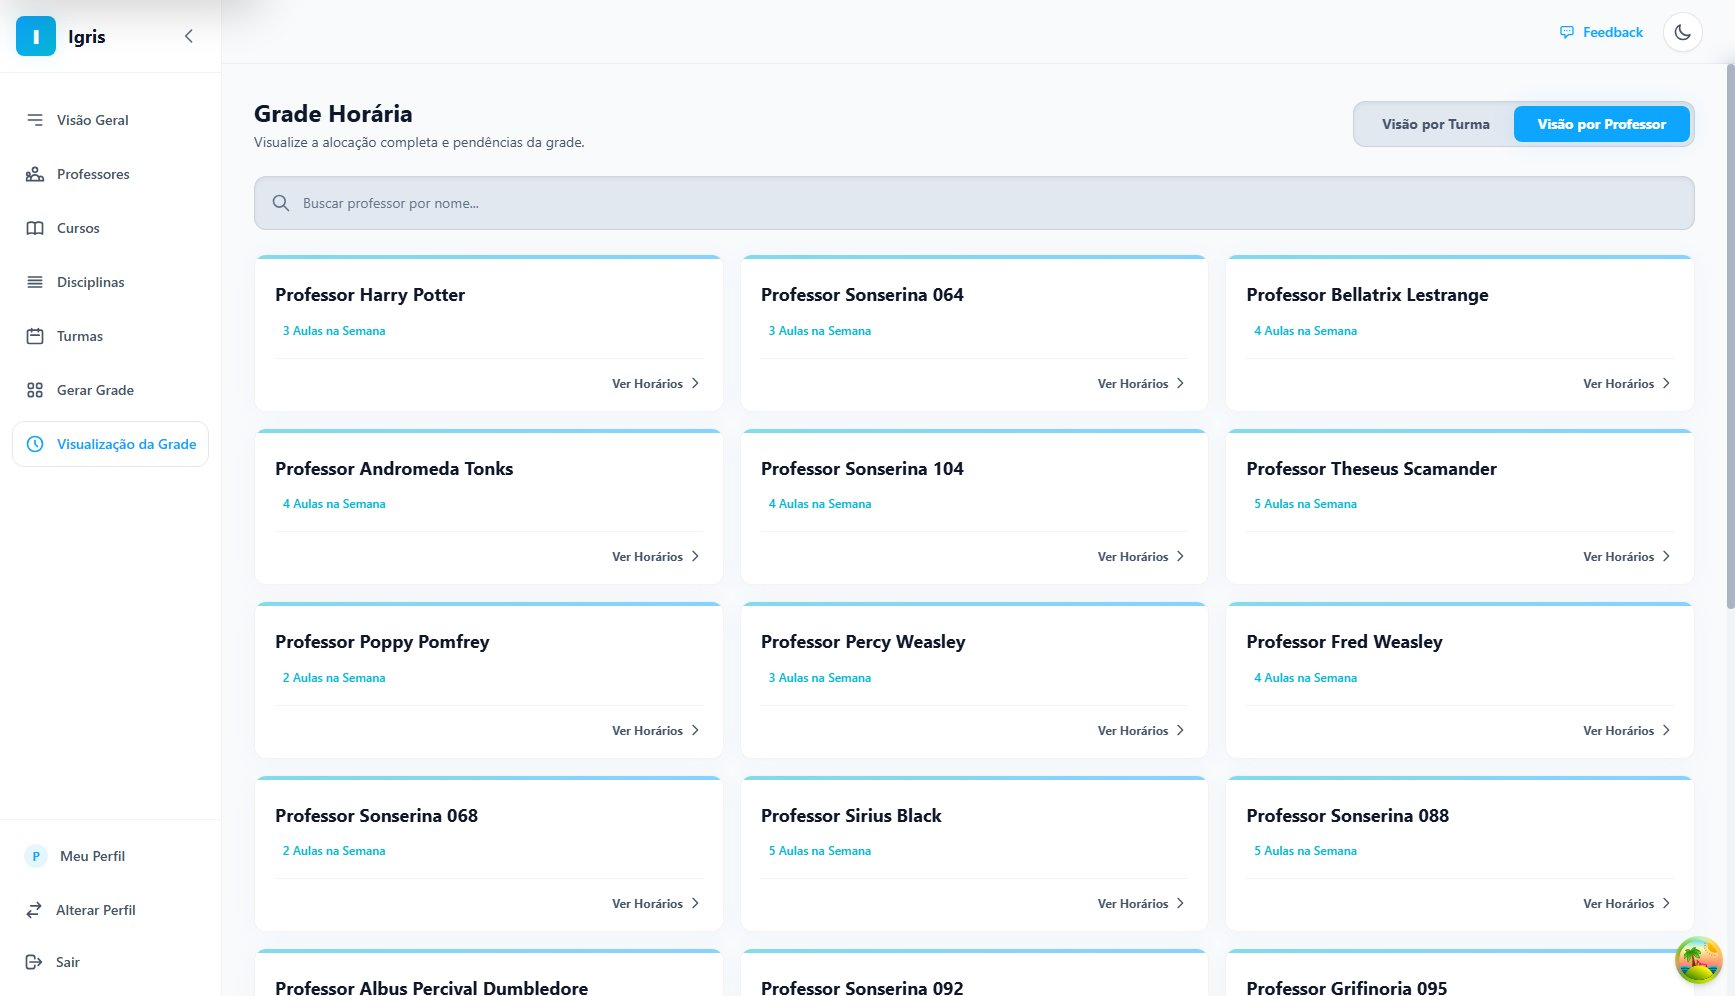
\includegraphics[width=\textwidth]{figuras/paginas/Figura_39_PG24.jpg}
\fonteautores
\end{figure}

A visão por professor organiza a grade horária em cartões individuais para cada docente. Cada cartão apresenta a quantidade de aulas atribuídas na semana e fornece acesso ao detalhamento dos horários, permitindo ao coordenador acompanhar a distribuição da carga docente.

\begin{tabelainteracoes}{Interações da Grade Horária -- Visão por Professor}{tab:interacoes-grade-professor-consulta}
Selecionar ``Visão por Professor'' & O sistema agrupa as aulas da grade ativa por docente. & A quantidade exibida deve considerar somente o período letivo selecionado. \\
\hline
Pesquisar pelo nome do professor & O sistema filtra os cartões conforme o texto informado. & Quando não houver correspondência, deve ser apresentada uma indicação de lista vazia. \\
\hline
Consultar a quantidade de aulas semanais & O sistema apresenta a carga atribuída a cada professor. & O valor auxilia a identificar professores com carga reduzida ou excessiva. \\
\hline
Clicar em ``Ver Horários'' & O sistema abre a matriz semanal do professor selecionado. & O detalhamento deve mostrar apenas as aulas vinculadas ao docente acionado. \\
\hline
Alternar para ``Visão por Turma'' & O sistema reorganiza a mesma grade em cartões de turmas. & A mudança de visualização não modifica as alocações armazenadas. \\
\hline
\end{tabelainteracoes}

% PG25.jpg
\begin{figure}[H]
\centering
\caption{Grade Horária - Detalhamento Semanal do Professor}
\label{fig:PG25}
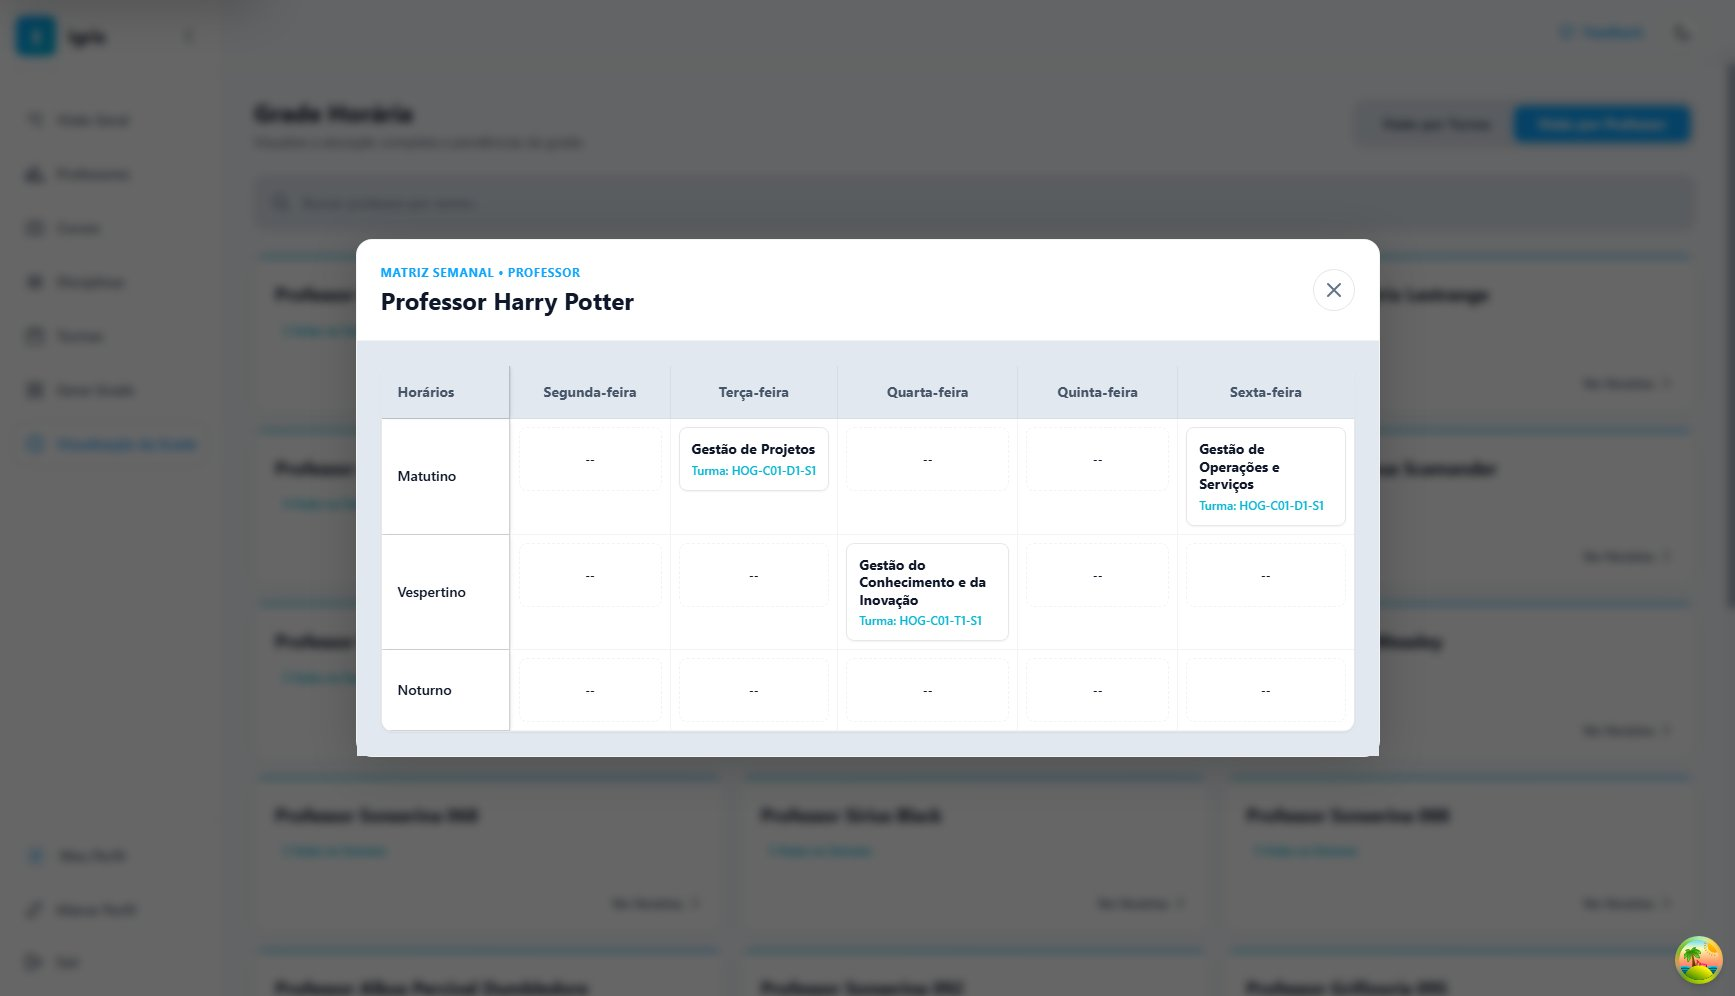
\includegraphics[width=\textwidth]{figuras/paginas/Figura_40_PG25.jpg}
\fonteautores
\end{figure}

A janela apresenta a matriz semanal de um professor selecionado, distribuindo suas aulas entre os dias da semana e os turnos letivos. Cada horário preenchido identifica a disciplina ministrada e a turma correspondente, oferecendo uma visão individual da carga docente.

\begin{tabelainteracoes}{Interações do Detalhamento Semanal do Professor}{tab:interacoes-detalhamento-semanal-professor}
Abrir os horários de um professor & O sistema apresenta a matriz semanal e identifica o docente no cabeçalho. & Os dados devem corresponder à grade ativa e ao período letivo consultado. \\
\hline
Consultar uma célula preenchida & O sistema exibe a disciplina e a turma atribuídas ao professor naquele horário. & A alocação deve respeitar a disponibilidade e as áreas de atuação cadastradas. \\
\hline
Consultar uma célula vazia & O sistema indica que não existe aula atribuída naquele intervalo. & Um período sem aula não representa necessariamente disponibilidade para novas alocações. \\
\hline
Identificar aulas simultâneas & O sistema deve sinalizar a sobreposição para correção. & Um professor não pode ministrar aulas para turmas diferentes no mesmo horário. \\
\hline
Clicar no ícone de fechar & O sistema encerra o detalhamento e retorna à visão por professores. & Fechar a janela não modifica a grade. \\
\hline
\end{tabelainteracoes}

% PG26.jpg
\begin{figure}[H]
\centering
\caption{Painel Acadêmico - Áreas de Atuação do Professor}
\label{fig:PG26}
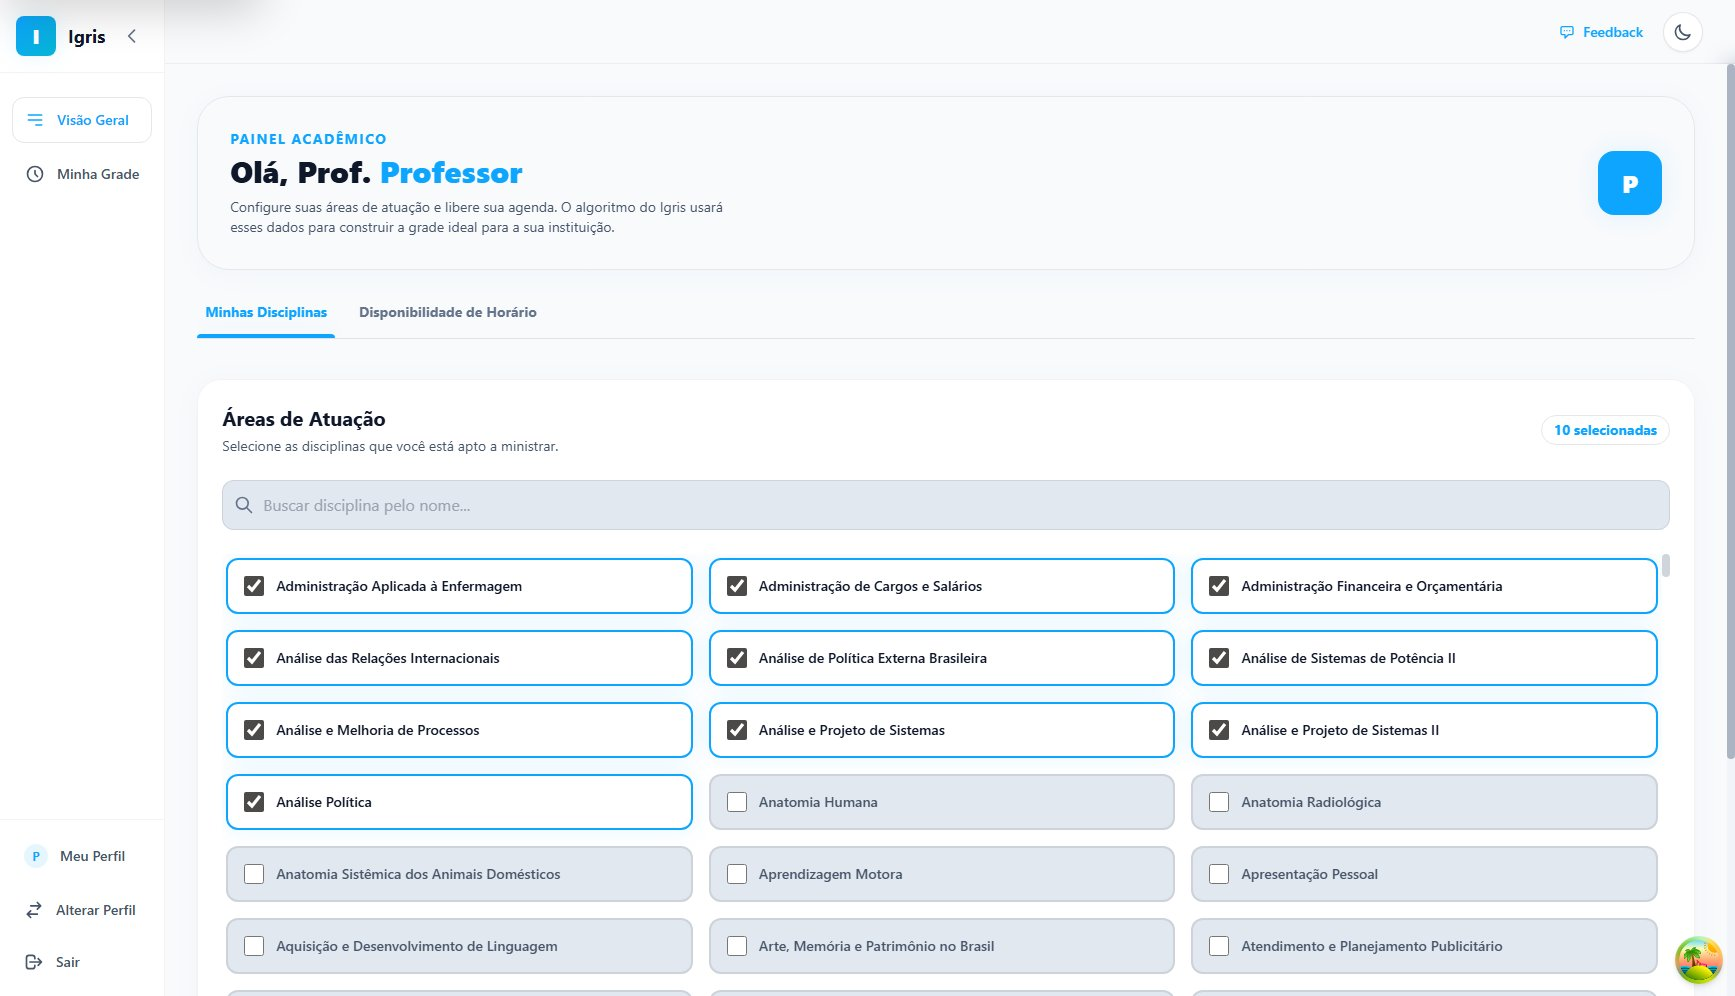
\includegraphics[width=\textwidth]{figuras/paginas/Figura_41_PG26.jpg}
\fonteautores
\end{figure}

No painel acadêmico, a aba ``Minhas Disciplinas'' permite ao professor consultar e selecionar suas áreas de atuação. As disciplinas são apresentadas com caixas de seleção e uma ferramenta de busca, fornecendo ao algoritmo as informações necessárias para realizar alocações compatíveis com a qualificação do docente.

\begin{tabelainteracoes}{Interações das Áreas de Atuação no Painel do Professor}{tab:interacoes-areas-painel-professor}
Selecionar a aba ``Minhas Disciplinas'' & O sistema apresenta as disciplinas disponíveis e destaca aquelas já vinculadas ao professor. & As seleções representam as matérias que o docente está habilitado a ministrar. \\
\hline
Pesquisar uma disciplina & O sistema filtra a relação conforme o termo informado. & As disciplinas selecionadas devem permanecer marcadas mesmo quando não estiverem visíveis no filtro atual. \\
\hline
Marcar uma disciplina & O sistema adiciona a matéria às áreas de atuação do professor. & O vínculo passa a ser considerado pelo algoritmo nas futuras alocações docentes. \\
\hline
Desmarcar uma disciplina & O sistema remove a matéria das áreas de atuação selecionadas. & Se existirem alocações vigentes para a disciplina, o sistema deve alertar sobre o impacto da alteração. \\
\hline
Consultar o total de disciplinas selecionadas & O sistema atualiza o contador apresentado na seção. & O valor facilita a conferência das áreas atualmente associadas ao professor. \\
\hline
Selecionar a aba ``Disponibilidade do Professor'' & O sistema abre o mapa semanal para consulta e manutenção dos horários livres. & As áreas de atuação e a disponibilidade são restrições complementares utilizadas na geração da grade. \\
\hline
\end{tabelainteracoes}

% PG27.jpg
\begin{figure}[H]
\centering
\caption{Áreas de Atuação do Professor}
\label{fig:PG27}
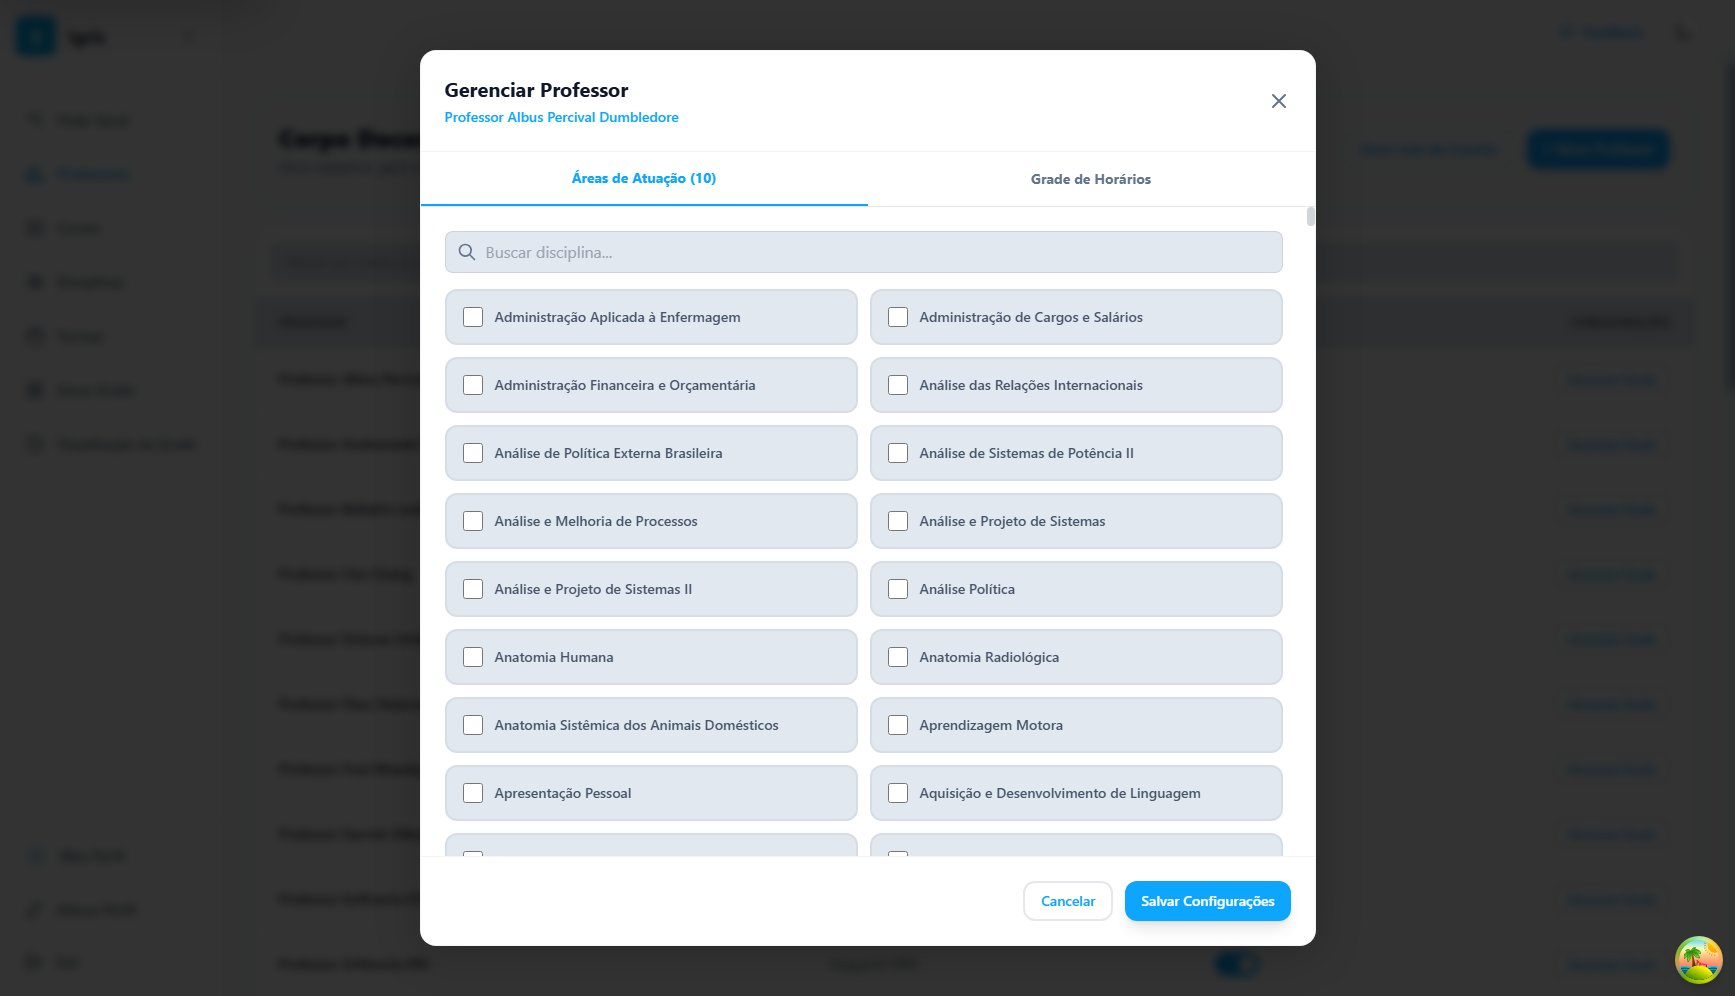
\includegraphics[width=\textwidth]{figuras/paginas/Figura_42_PG27.jpg}
\fonteautores
\end{figure}

O coordenador tem acesso a uma janela de configuração onde define quais disciplinas o professor está habilitado a ministrar, permitindo uma restrição correta baseada nas qualificações.

\begin{tabelainteracoes}{Interações das Áreas de Atuação do Professor}{tab:interacoes-areas-professor}
Pesquisar uma disciplina & O sistema filtra as opções de áreas de atuação disponíveis. & As disciplinas já selecionadas devem permanecer marcadas mesmo quando estiverem fora do filtro atual. \\
\hline
Marcar uma disciplina & O sistema inclui temporariamente a matéria entre as áreas que o professor pode ministrar. & A seleção será considerada como restrição de aptidão nas próximas gerações de grade. \\
\hline
Desmarcar uma disciplina & O sistema remove temporariamente a matéria da lista de habilitações do docente. & Se houver alocações existentes nessa disciplina, o sistema deve alertar sobre o possível impacto. \\
\hline
Clicar em ``Salvar Configurações'' & O sistema persiste os vínculos entre professor e disciplinas e fecha a janela. & A confirmação deve ser exibida e as mudanças devem afetar somente o professor selecionado. \\
\hline
Clicar em ``Cancelar'' ou fechar & O sistema descarta alterações não salvas e retorna à tela anterior. & As áreas previamente armazenadas permanecem inalteradas. \\
\hline
\end{tabelainteracoes}

% PG28.jpg
\begin{figure}[H]
\centering
\caption{Parâmetros do Sistema (Sunny) - Desempenho Rápido}
\label{fig:PG28}
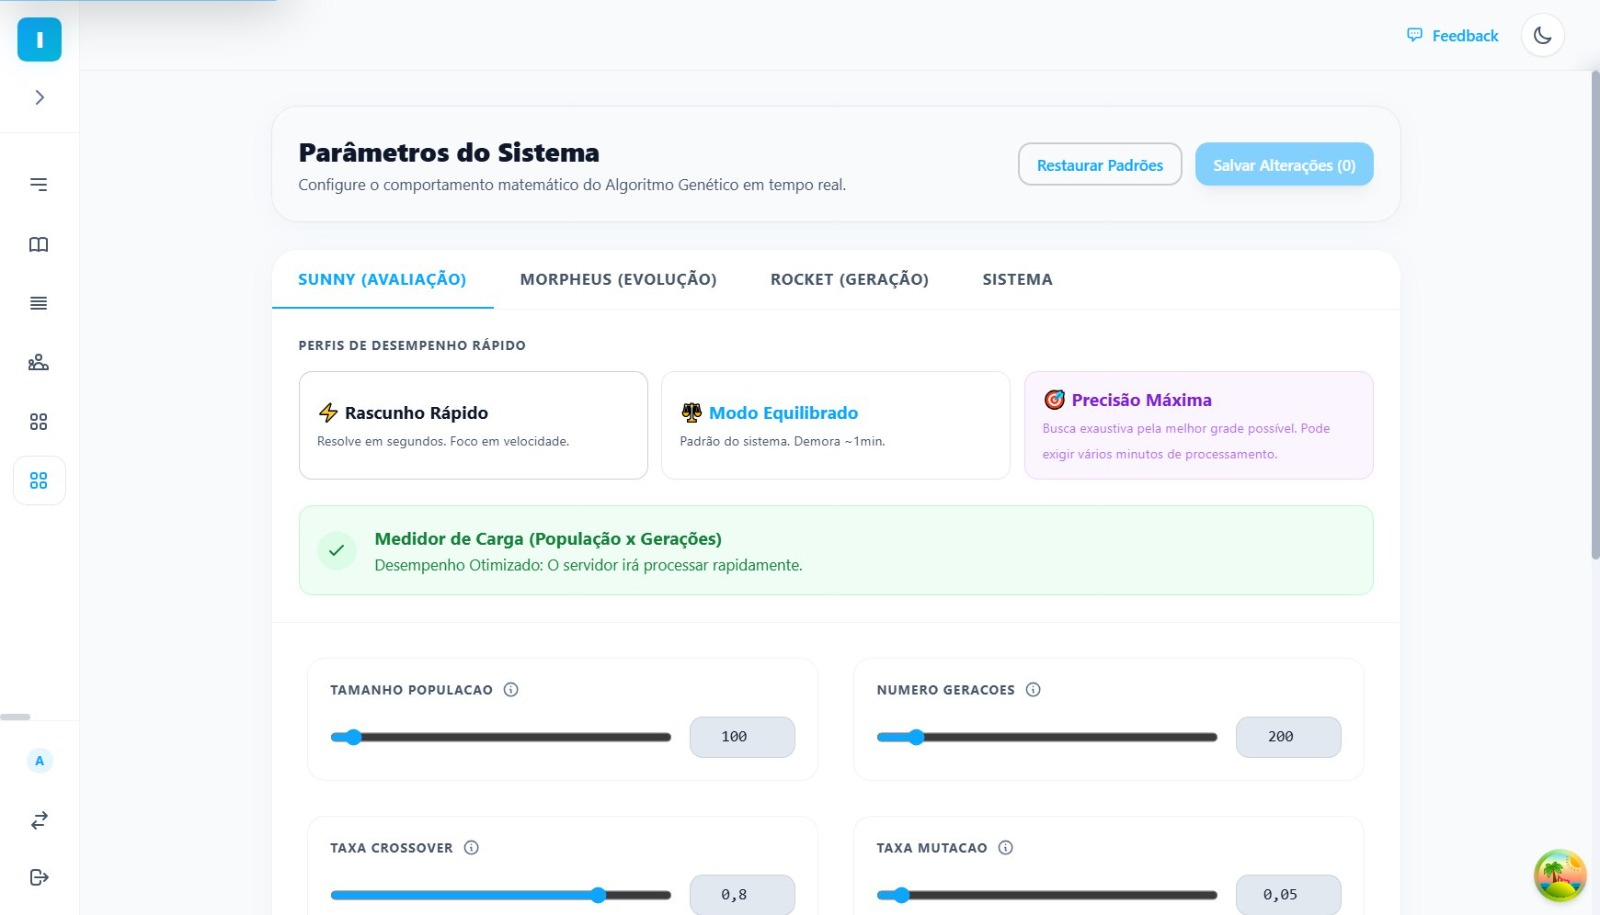
\includegraphics[width=\textwidth]{figuras/paginas/Figura_43_PG28.jpg}
\fonteautores
\end{figure}

A tela oferece perfis de desempenho rápido (Rascunho Rápido, Modo Equilibrado e Modo Perfeição), simplificando a configuração matemática do algoritmo em predefinições.

\begin{tabelainteracoes}{Interações dos Parâmetros do Sistema -- Desempenho Rápido}{tab:interacoes-perfis-desempenho}
Selecionar ``Rascunho Rápido'' & O sistema aplica parâmetros voltados à obtenção de resultado em menor tempo. & A execução tende a consumir menos recursos, podendo produzir uma solução com qualidade inferior. \\
\hline
Selecionar ``Modo Equilibrado'' & O sistema aplica uma combinação intermediária entre tempo de processamento e qualidade. & É a opção recomendada para uso geral quando não há necessidade de ajuste manual. \\
\hline
Selecionar ``Modo Perfeição'' & O sistema aplica parâmetros mais intensivos para ampliar a busca por uma solução de maior qualidade. & O modo pode aumentar significativamente o tempo e o consumo computacional. \\
\hline
Alterar manualmente um parâmetro após escolher um perfil & O sistema atualiza o valor e passa a tratar a configuração como personalizada. & O medidor de carga deve ser recalculado imediatamente. \\
\hline
Clicar em ``Salvar Alterações'' & O sistema persiste o perfil e os valores apresentados para futuras execuções. & A configuração não deve modificar resultados ou grades já armazenados. \\
\hline
Clicar em ``Restaurar Padrões'' & O sistema repõe a predefinição padrão do algoritmo selecionado. & Uma confirmação evita a perda acidental de ajustes personalizados. \\
\hline
\end{tabelainteracoes}

% PG29.jpg
\begin{figure}[H]
\centering
\caption{Auditoria do Corpo de Coordenadores}
\label{fig:PG29}
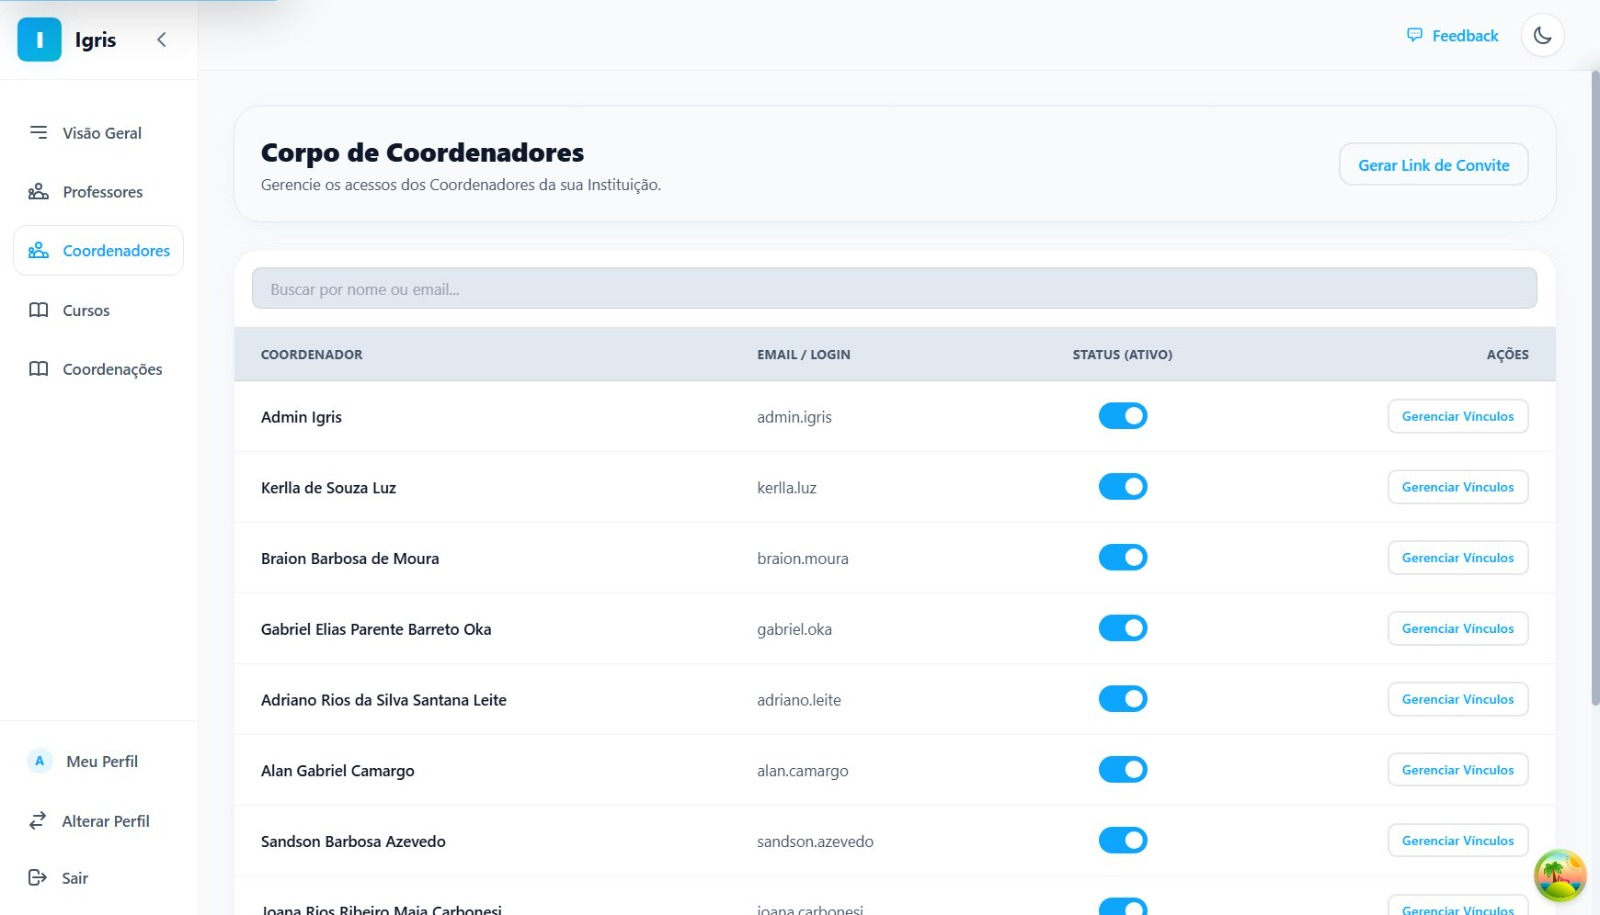
\includegraphics[width=\textwidth]{figuras/paginas/Figura_44_PG29.jpg}
\fonteautores
\end{figure}

Os acessos do quadro gestor institucional podem ser auditados e controlados através desta listagem centralizada, que promove transparência na gestão.

\begin{tabelainteracoes}{Interações da Auditoria do Corpo de Coordenadores}{tab:interacoes-auditoria-coordenadores}
Pesquisar um coordenador & O sistema filtra a lista pelo nome ou e-mail do gestor. & A consulta deve permanecer limitada à instituição administrada pelo usuário. \\
\hline
Consultar o status de acesso & O sistema apresenta se o perfil do coordenador está ativo ou inativo. & O status exibido deve refletir o valor atualmente persistido. \\
\hline
Ativar ou desativar um coordenador & O sistema atualiza a permissão de acesso e registra a alteração. & A auditoria deve preservar autor, data e estado alterado quando o sistema possuir histórico de ações. \\
\hline
Clicar em ``Ver Configuração'' & O sistema apresenta os perfis e coordenações associados ao usuário. & O administrador pode verificar se os privilégios concedidos são compatíveis com a função exercida. \\
\hline
Gerar um link de convite & O sistema cria um convite para inclusão de um novo gestor. & O ingresso do usuário deve permanecer sujeito às regras de validação e atribuição de coordenação. \\
\hline
\end{tabelainteracoes}

% PG30.jpg
\begin{figure}[H]
\centering
\caption{Adição e Atribuição de Coordenações}
\label{fig:PG30}
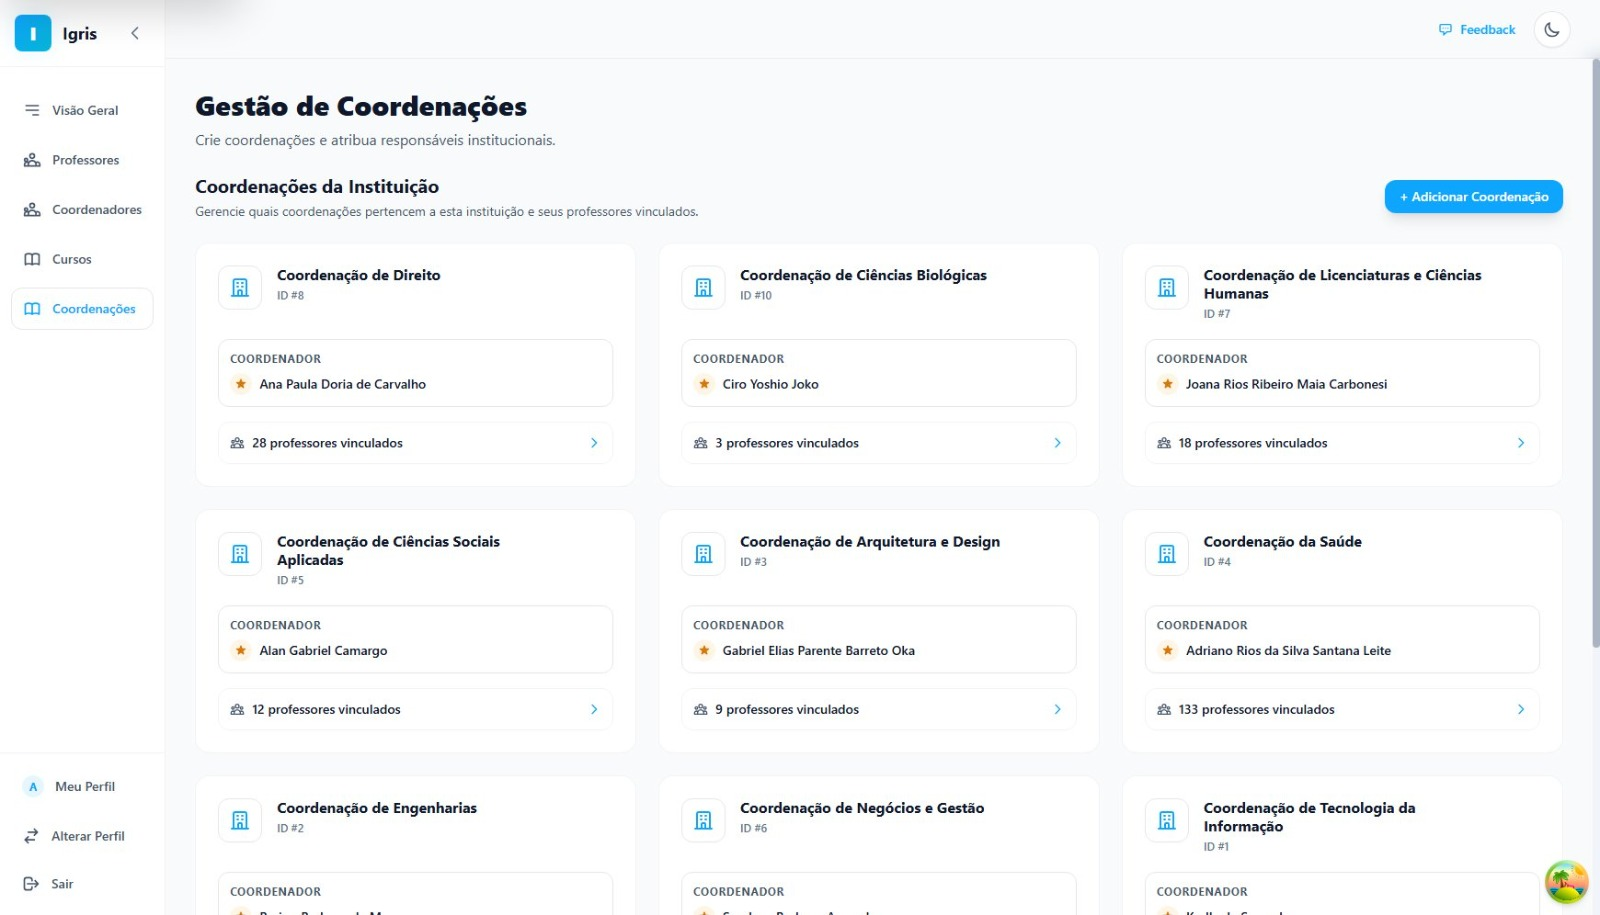
\includegraphics[width=\textwidth]{figuras/paginas/Figura_45_PG30.jpg}
\fonteautores
\end{figure}

A interface evidencia que os responsáveis podem ser rapidamente identificados e que novas áreas podem ser estruturadas com agilidade.

\begin{tabelainteracoes}{Interações da Adição e Atribuição de Coordenações}{tab:interacoes-adicao-coordenacoes}
Informar o nome da nova coordenação & O sistema prepara o cadastro de uma nova área institucional. & O nome deve ser obrigatório e não pode duplicar outra coordenação da mesma instituição. \\
\hline
Clicar em ``Adicionar'' & O sistema cria a coordenação e a inclui na tabela. & Uma mensagem deve confirmar a operação ou explicar a falha de validação. \\
\hline
Consultar os responsáveis de uma coordenação & O sistema apresenta os coordenadores atualmente vinculados à área. & A ausência de responsáveis deve ser sinalizada para evitar uma coordenação sem gestão definida. \\
\hline
Selecionar um coordenador para atribuição & O sistema cria o vínculo entre o usuário, seu perfil e a coordenação escolhida. & O usuário precisa possuir um cadastro válido e permissão compatível. \\
\hline
Remover um responsável & O sistema solicita confirmação e encerra o vínculo com a coordenação. & A remoção não exclui o usuário; se for o único responsável, o sistema deve alertar sobre a área ficar sem coordenador. \\
\hline
\end{tabelainteracoes}

% PG31.jpg
\begin{figure}[H]
\centering
\caption{Indicadores de Carga do Sistema e Algoritmo}
\label{fig:PG31}
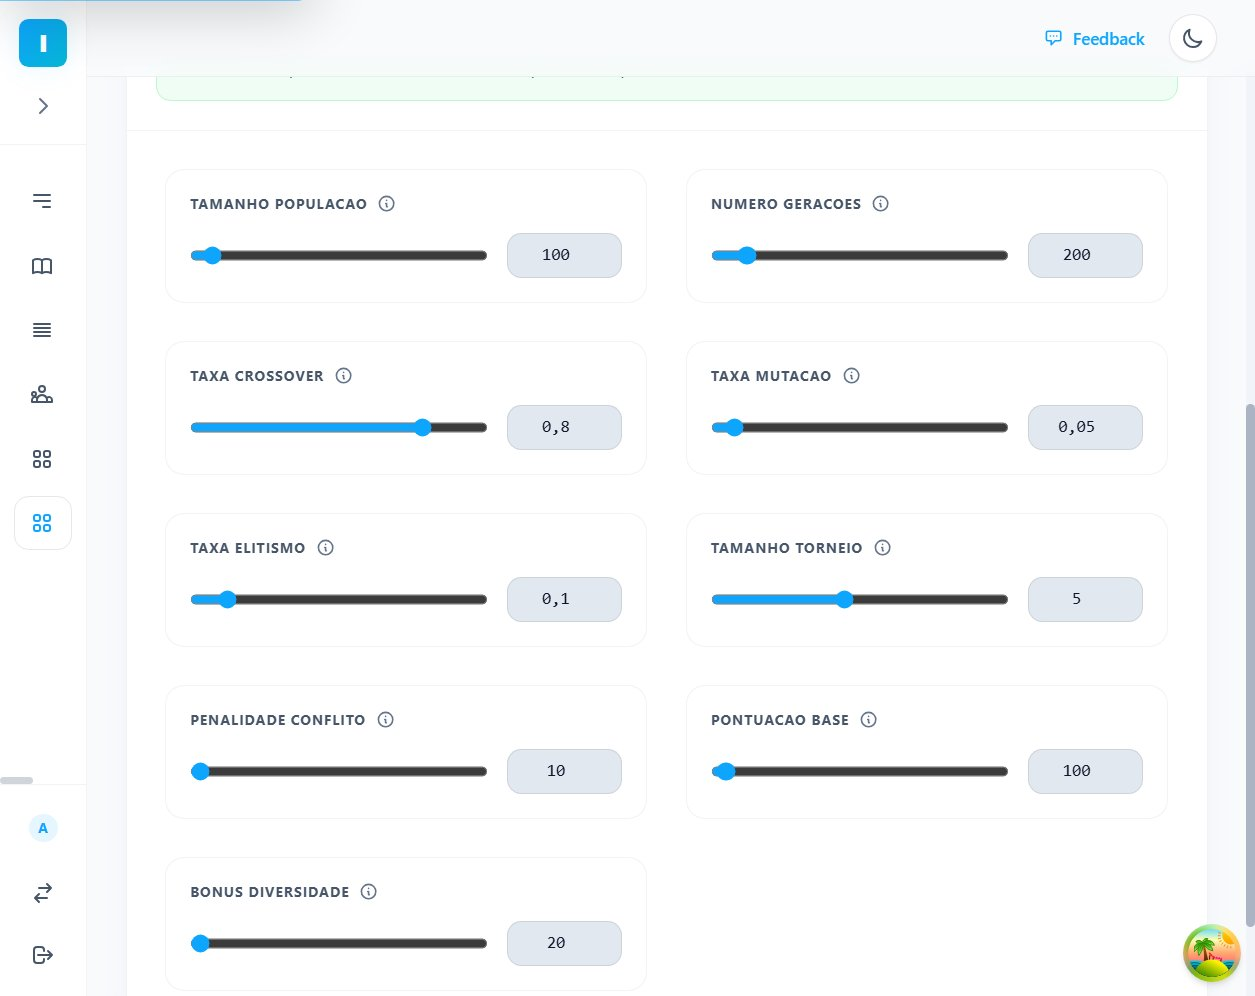
\includegraphics[width=\textwidth]{figuras/paginas/Figura_46_PG31.jpg}
\fonteautores
\end{figure}

O Medidor de Carga ajuda o gestor a equilibrar a eficiência do processamento algorítmico de forma que as interações funcionem sem sobrecarregar a infraestrutura da nuvem.

\begin{tabelainteracoes}{Interações dos Indicadores de Carga do Sistema e Algoritmo}{tab:interacoes-indicadores-carga}
Mover os controles de população ou gerações & O sistema atualiza os valores e recalcula a carga estimada da execução. & Aumentar esses parâmetros amplia o espaço de busca e normalmente eleva o tempo de processamento. \\
\hline
Ajustar taxas evolutivas e penalidades & O sistema atualiza a configuração matemática do algoritmo. & Cada controle deve respeitar sua faixa válida e exibir o valor exato aplicado. \\
\hline
Consultar o indicador superior & O sistema apresenta uma avaliação textual e visual da configuração atual. & A cor e a mensagem devem permitir reconhecer rapidamente uma carga segura ou elevada. \\
\hline
Definir valores potencialmente excessivos & O sistema alerta sobre risco de demora ou sobrecarga antes do salvamento ou da execução. & Limites críticos podem ser bloqueados conforme a capacidade da infraestrutura. \\
\hline
Salvar os parâmetros & O sistema persiste a configuração para as próximas gerações de grade. & O salvamento deve invalidar configurações em cache para que os motores recebam os novos valores. \\
\hline
\end{tabelainteracoes}

% PG32.jpg
\begin{figure}[H]
\centering
\caption{Disponibilidade Semanal do Professor pelo Coordenador}
\label{fig:PG32}
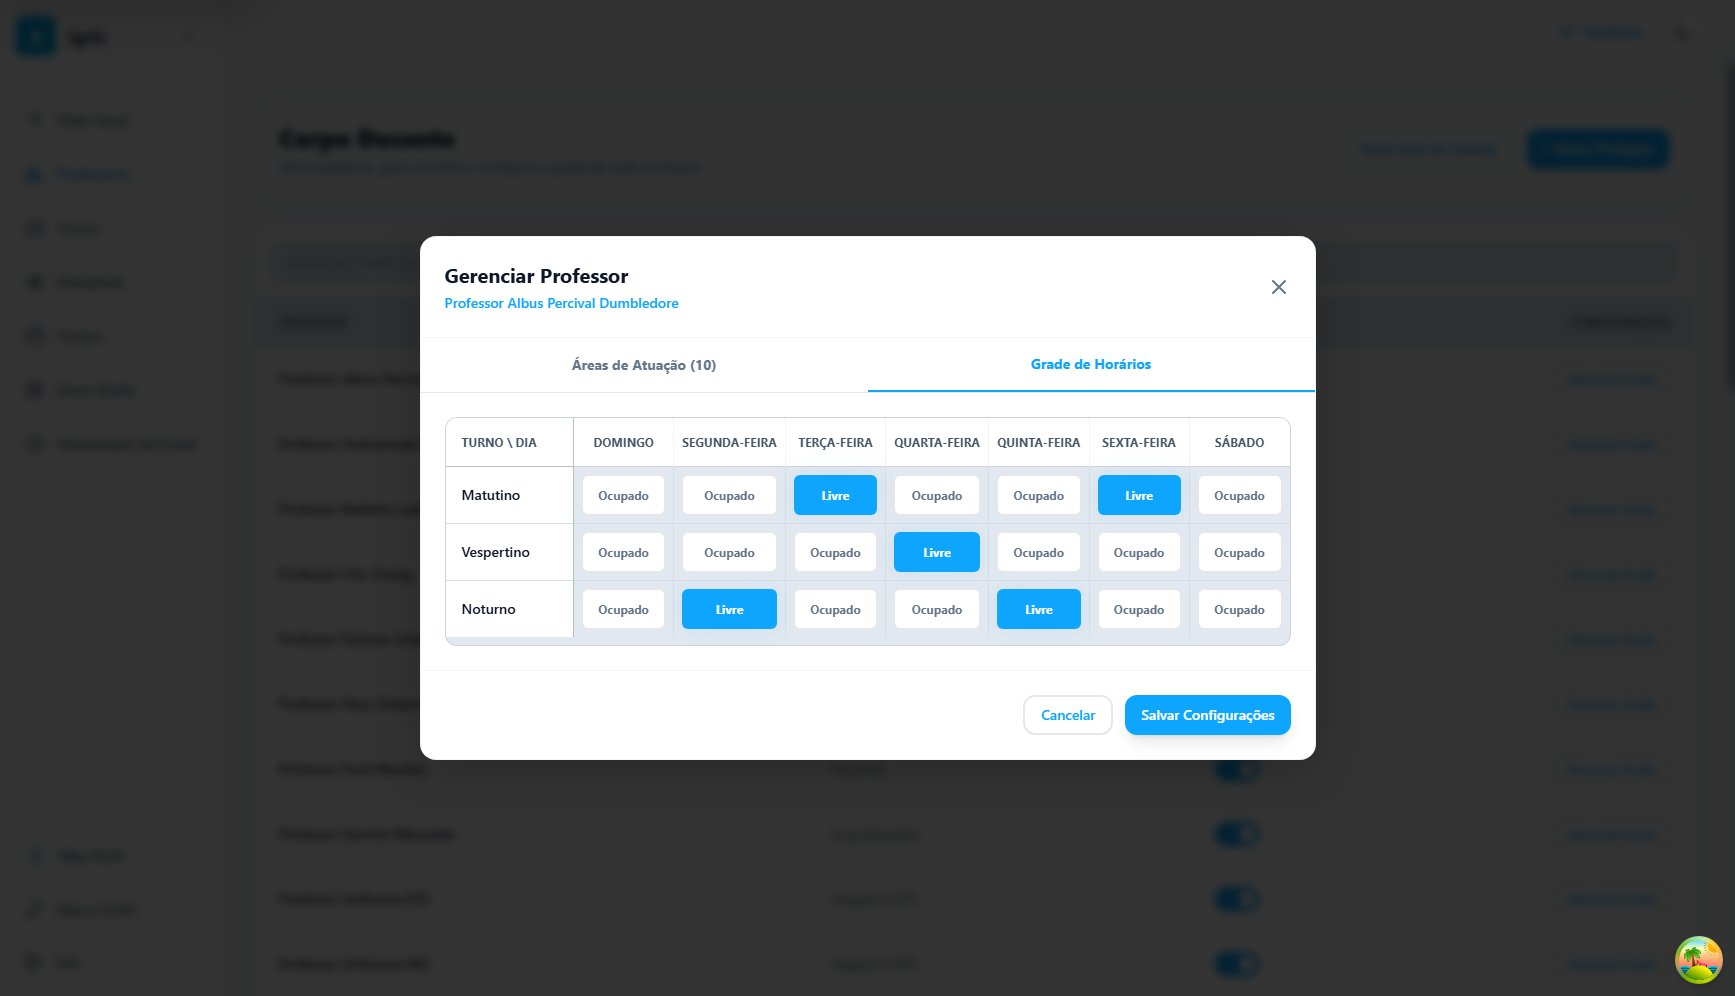
\includegraphics[width=\textwidth]{figuras/paginas/Figura_47_PG32.jpg}
\fonteautores
\end{figure}

A aba Grade de Horários permite ao coordenador visualizar e estabelecer as restrições semanais de disponibilidade de um docente, separadas por dias e turnos.

\begin{tabelainteracoes}{Interações da Disponibilidade Semanal do Professor pelo Coordenador}{tab:interacoes-disponibilidade-coordenador}
Selecionar a aba ``Grade de Horários'' & O sistema apresenta a disponibilidade semanal do professor em uma matriz de dias e turnos. & A janela deve manter a identificação do docente selecionado. \\
\hline
Clicar em um horário ocupado ou indisponível & O sistema alterna o período para livre, quando a alteração for permitida. & A representação visual deve distinguir claramente os estados ``Livre'' e ``Ocupado''. \\
\hline
Clicar em um horário livre & O sistema alterna o período para ocupado ou indisponível. & A mudança é temporária até que as configurações sejam salvas. \\
\hline
Clicar em ``Salvar Configurações'' & O sistema valida e persiste a disponibilidade do professor. & Duplicidades devem ser evitadas e alterações que afetem uma grade já ativa podem exigir alerta. \\
\hline
Clicar em ``Cancelar'' ou fechar & O sistema descarta as mudanças não salvas e retorna ao gerenciamento docente. & A disponibilidade anteriormente registrada permanece inalterada. \\
\hline
\end{tabelainteracoes}

% PG33.jpg
\begin{figure}[H]
\centering
\caption{Painel Acadêmico - Mapa de Disponibilidade do Professor}
\label{fig:PG33}
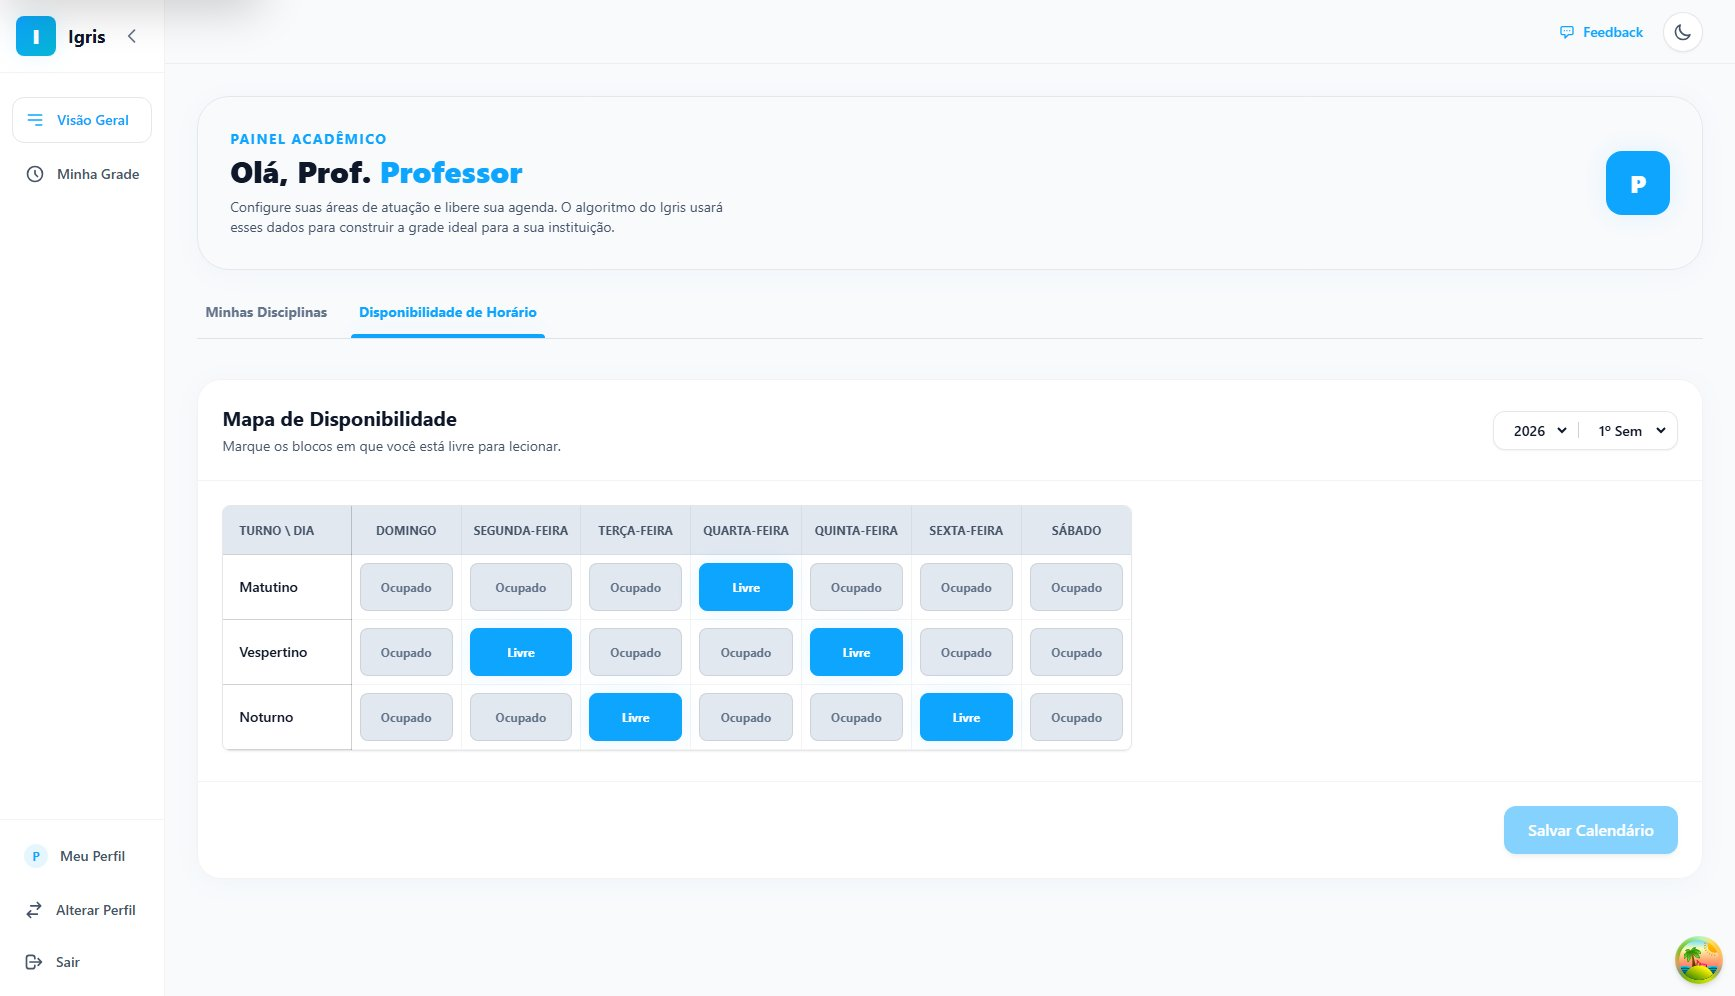
\includegraphics[width=\textwidth]{figuras/paginas/Figura_48_PG33.jpg}
\fonteautores
\end{figure}

No acesso exclusivo do professor, o Mapa de Disponibilidade e a seleção das Áreas de Atuação são centralizados, permitindo que o docente preencha sua matriz semanal autonomamente.

\begin{tabelainteracoes}{Interações do Painel Acadêmico -- Mapa de Disponibilidade do Professor}{tab:interacoes-mapa-disponibilidade-professor}
Selecionar ano e semestre & O sistema carrega a disponibilidade correspondente ao período letivo escolhido. & A manutenção deve ocorrer separadamente para cada combinação de ano e semestre. \\
\hline
Clicar em um bloco da matriz semanal & O sistema alterna o estado do horário entre livre e ocupado. & O estado visual deve ser atualizado imediatamente, mas a alteração só se torna definitiva após o salvamento. \\
\hline
Clicar em ``Salvar Calendário'' & O sistema verifica duplicidades e persiste a disponibilidade informada pelo professor. & Uma mensagem deve confirmar o salvamento; falhas devem manter os dados na tela para nova tentativa. \\
\hline
Trocar de período com alterações não salvas & O sistema alerta sobre a possível perda das modificações antes de carregar outro calendário. & O usuário deve poder cancelar a troca e salvar os dados atuais. \\
\hline
Selecionar a aba ``Minhas Disciplinas'' & O sistema apresenta as áreas de atuação vinculadas ao professor. & A lista permite consultar as disciplinas consideradas pelo algoritmo nas alocações docentes. \\
\hline
Não existir configuração para o período & O sistema apresenta a matriz inicial vazia ou padrão para preenchimento. & Nenhum horário deve ser considerado disponível sem confirmação do professor, conforme a regra institucional. \\
\hline
\end{tabelainteracoes}


\chapter{Benchmark}
\label{cap:benchmark}

Neste capítulo, são apresentados os experimentos realizados para avaliar o desempenho dos algoritmos Morpheus, Sunny e Rocket na geração automática de grades horárias acadêmicas do sistema IGRIS. O objetivo do benchmark é comparar o comportamento das três implementações diante do mesmo conjunto de testes, considerando métricas como tempo de execução, consumo de memória, número de gerações executadas, ocorrência de parada antecipada, score final e erro médio.

A comparação entre os algoritmos é necessária porque todos têm a mesma finalidade dentro do sistema: produzir uma grade horária acadêmica a partir das informações disponíveis sobre turmas, disciplinas, professores e horários. Entretanto, apesar de resolverem o mesmo problema, as implementações possuem características diferentes em relação à arquitetura, à organização interna dos dados, ao tratamento de conflitos, ao critério de parada e ao consumo de recursos computacionais.

Foram analisados dois cenários de execução, identificados nos relatórios como i3 e i5/full. Em ambos os casos, os algoritmos foram submetidos a execuções repetidas com variações de parâmetros evolutivos. Dessa forma, a análise não se limita a uma única execução isolada, mas considera o comportamento geral das implementações ao longo de diferentes configurações do algoritmo genético.

A comparação realizada neste capítulo não deve ser entendida como uma avaliação genérica entre linguagens de programação, arquiteturas ou tecnologias. O foco está nas três implementações concretas utilizadas no IGRIS. Portanto, os resultados discutidos dizem respeito ao comportamento observado no protocolo de benchmark executado, com os parâmetros, dados e ambiente disponíveis nos relatórios analisados.

\section{Sobre o Benchmark}
\label{sec:sobre-o-benchmark}

Para avaliar os algoritmos Morpheus, Sunny e Rocket, foi utilizado um benchmark progressivo composto por dois cenários principais. O primeiro cenário é identificado como i3, enquanto o segundo é identificado como i5/full. Em cada cenário, os três algoritmos foram executados repetidamente, permitindo observar diferenças de desempenho, estabilidade e consumo de recursos.

Os cenários i3 e i5/full representam presets distintos de capacidade computacional. O cenário i3 foi utilizado como ambiente de capacidade reduzida, simulando uma configuração com menor disponibilidade de processamento. Nos scripts de execução analisados, esse preset foi operacionalizado por meio de limitação de CPU nos containers, com o comando \texttt{docker update --cpus 4} aplicado aos serviços avaliados antes da execução do benchmark. O cenário i5/full, por sua vez, foi utilizado como ambiente de capacidade total, no qual os containers foram executados sem limite explícito de CPU, indicado nos scripts pela restauração do parâmetro para \texttt{--cpus 0}. Assim, a comparação entre i3 e i5/full também permite observar como cada algoritmo responde à ampliação de capacidade de processamento disponível.

A escolha desses dois cenários teve finalidade metodológica específica. O cenário i3 foi utilizado para testar o comportamento dos algoritmos sob restrição de processamento, isto é, em uma condição mais próxima de implantação econômica ou de infraestrutura compartilhada. O cenário i5/full foi utilizado como referência de capacidade ampliada, permitindo observar se a remoção do limite de CPU reduziria proporcionalmente a latência ou se os algoritmos permaneceriam limitados por outros fatores, como custo da função \textit{fitness}, estruturas de dados, sincronização, alocação de memória ou critérios de parada. A hipótese técnica subjacente era que implementações mais eficientes deveriam manter estabilidade no ambiente restrito e, ao mesmo tempo, converter parte da capacidade adicional do ambiente i5/full em menor tempo de resposta. Dessa forma, a comparação não mede apenas qual algoritmo é mais rápido, mas também a sensibilidade de cada implementação à disponibilidade de recursos computacionais.

Quanto à memória RAM, os relatórios registram o consumo por meio da telemetria do \texttt{docker stats} durante cada requisição. Os artefatos de execução não apresentam um limite explícito de memória por container, como \texttt{docker update --memory}, \texttt{mem\_limit} ou configuração equivalente no \texttt{docker-compose}. Dessa forma, a RAM deve ser interpretada como capacidade disponível do ambiente monitorado, e não como cota fixa documentada por serviço. Pelos percentuais de memória reportados nos CSVs, a capacidade total observada pelo Docker ficou próxima de 8 GB nos testes analisados. Portanto, o preset i3 deve ser descrito como cenário de processamento reduzido, com 4 CPUs disponíveis para os containers avaliados, enquanto o preset i5/full deve ser descrito como cenário de processamento total, sem limitação explícita de CPU e com a memória disponível do ambiente Docker monitorado.

O volume de 9.000 requisições por algoritmo em cada cenário foi adotado para reduzir a influência de execuções isoladas e permitir uma leitura mais estável das métricas agregadas. Em algoritmos genéticos, a presença de componentes estocásticos pode produzir variações entre execuções mesmo quando o \textit{payload} e os parâmetros permanecem equivalentes. Um conjunto de 9.000 amostras aumenta a robustez descritiva da média e, principalmente, torna mais informativo o percentil 95: nesse caso, a cauda superior da distribuição ainda contém aproximadamente 450 observações, evitando que o p95 seja definido por poucos casos extremos. Além disso, o volume escolhido preserva viabilidade prática de execução, pois permite repetir o experimento para três algoritmos, dois cenários e múltiplas configurações paramétricas sem tornar o tempo total do benchmark incompatível com a coleta operacional.

Os parâmetros avaliados no benchmark foram: taxa de \textit{crossover}, tamanho da população, número de gerações, taxa de elitismo, pontuação base, penalidade de conflito, bônus de diversidade, tamanho do torneio e taxa de mutação. Esses parâmetros foram escolhidos porque influenciam diretamente o comportamento de um algoritmo genético, afetando a forma como a população evolui, como os indivíduos são selecionados, como novas soluções são geradas e como conflitos são penalizados.

As métricas utilizadas na avaliação foram: latência média, percentil 95 da latência, uso médio de CPU, pico de CPU, uso médio de memória RAM, pico de memória RAM, custo composto tempo \(\times\) memória, número médio de gerações executadas, melhor geração média, ocorrência de parada antecipada, score final e erro médio. A partir dessas métricas, torna-se possível analisar tanto o custo operacional dos algoritmos quanto a qualidade relativa das soluções geradas.

A latência média indica o tempo médio de resposta das execuções. O percentil 95, identificado como p95, representa o tempo abaixo do qual se encontram 95\% das execuções, sendo útil para observar o comportamento das execuções mais lentas. O uso de RAM e CPU permite avaliar o custo computacional das implementações. Já as métricas de gerações, score, erro médio e parada antecipada permitem analisar o comportamento evolutivo dos algoritmos.

Formalmente, para um conjunto de \(n\) execuções válidas de um algoritmo em determinado cenário, seja \(L_i\) a latência da \(i\)-ésima requisição, medida em milissegundos. A latência média é dada por:

\begin{equation}
L_{\text{média}} = \frac{1}{n}\sum_{i=1}^{n} L_i.
\end{equation}

Para o cálculo do percentil 95, as latências são ordenadas de forma crescente, produzindo a sequência \(L_{(1)} \leq L_{(2)} \leq \cdots \leq L_{(n)}\). O p95 é então aproximado pelo valor na posição \(k = \lceil 0{,}95n \rceil\), isto é:

\begin{equation}
p95 = L_{(k)}, \quad \text{com } k = \lceil 0{,}95n \rceil.
\end{equation}

Assim, quando \(n = 9.000\), o p95 corresponde aproximadamente à 8.550ª observação ordenada, indicando o limite abaixo do qual se situam 95\% das requisições medidas. Essa métrica complementa a média porque reduz o risco de interpretação baseada apenas no comportamento central da distribuição, evidenciando também a experiência das execuções mais lentas.

O uso médio de memória RAM segue a mesma lógica de agregação. Seja \(M_i\) o consumo de memória observado durante a \(i\)-ésima execução, em megabytes. A RAM média é calculada por:

\begin{equation}
\text{RAM}_{\text{média}} = \frac{1}{n}\sum_{i=1}^{n} M_i.
\end{equation}

O pico de memória, por sua vez, corresponde ao maior valor observado no conjunto de execuções:

\begin{equation}
\text{RAM}_{\text{pico}} = \max(M_1, M_2, \ldots, M_n).
\end{equation}

De maneira análoga, se \(C_i\) representa o uso de CPU observado na \(i\)-ésima execução, o uso médio e o pico de CPU são calculados por:

\begin{align}
\text{CPU}_{\text{média}} &= \frac{1}{n}\sum_{i=1}^{n} C_i,\\
\text{CPU}_{\text{pico}} &= \max(C_1, C_2, \ldots, C_n).
\end{align}

Na telemetria do \texttt{docker stats}, o percentual de CPU deve ser interpretado como uso agregado por núcleo lógico. Assim, 100\% de CPU equivale aproximadamente ao uso integral de um núcleo lógico durante a janela de amostragem. Em ambientes com múltiplos núcleos, valores acima de 100\% podem ocorrer quando o container utiliza mais de um núcleo simultaneamente. Portanto, essa métrica não representa necessariamente a ocupação de 100\% de todo o host físico, mas sim o consumo agregado observado para o container monitorado.

Para as métricas evolutivas, se \(G_i\) representa o número de gerações executadas na \(i\)-ésima requisição, então:

\begin{equation}
G_{\text{média}} = \frac{1}{n}\sum_{i=1}^{n} G_i.
\end{equation}

A taxa de sucesso também é calculada por proporção simples:

\begin{equation}
\text{Sucesso} = \frac{n_{\text{sucesso}}}{n_{\text{total}}}\times 100,
\end{equation}

em que \(n_{\text{sucesso}}\) é o número de requisições concluídas corretamente e \(n_{\text{total}}\) é o número total de requisições executadas no cenário.

Quando o benchmark utiliza o custo composto tempo \(\times\) memória, a métrica pode ser expressa como o produto entre latência média e RAM média:

\begin{equation}
C_{tm} = L_{\text{média}}\times \text{RAM}_{\text{média}}.
\end{equation}

Esse custo composto não substitui as métricas individuais, mas ajuda a identificar situações em que um algoritmo é simultaneamente lento e intensivo em memória. Duas implementações com latências semelhantes, por exemplo, podem ter custos operacionais distintos se uma delas exigir muito mais RAM para produzir resultado equivalente.

O score representa a pontuação associada à função \textit{fitness}. Como a função utiliza penalidades para conflitos e inconsistências, valores menos negativos indicam melhor avaliação relativa. O erro médio representa a quantidade média de inconsistências restantes nas soluções finais. Entretanto, os relatórios analisados não detalham completamente a composição desse erro para todos os algoritmos, ou seja, não permitem afirmar, de forma homogênea, se ele corresponde a conflitos de professor, conflitos de turma, demandas não alocadas ou combinação desses fatores.

De forma geral, a função de score pode ser descrita como uma combinação entre uma pontuação base, eventuais bônus e penalidades aplicadas às violações de restrições. Se \(B\) representa a pontuação base da solução, \(D\) representa o bônus de diversidade, \(v_j\) representa a quantidade de violações do tipo \(j\) e \(\lambda_j\) representa o peso ou a penalidade associada a esse tipo de violação, então o score pode ser representado por:

\begin{equation}
\text{Score} = B + D - \sum_{j=1}^{m}\lambda_j v_j.
\end{equation}

Nessa formulação, \(m\) é o número de categorias de restrição consideradas pela função \textit{fitness}. Quanto maior o número de violações ou maior o peso associado a elas, menor tende a ser o score final. Por isso, no benchmark, scores menos negativos indicam soluções relativamente melhores segundo a função \textit{fitness} implementada, embora não garantam, isoladamente, validade acadêmica completa da grade. O erro médio pode ser expresso por:

\begin{equation}
E_{\text{média}} = \frac{1}{n}\sum_{i=1}^{n} E_i,
\end{equation}

em que \(E_i\) representa o número de inconsistências remanescentes na solução final da \(i\)-ésima execução. Essa métrica aproxima a qualidade final das soluções, mas sua interpretação permanece limitada quando os relatórios não discriminam a natureza de cada inconsistência.

\section{Resultados Gerais}
\label{sec:resultados-gerais}

A Tabela~\ref{tab:resultados-gerais-benchmark} apresenta a síntese dos resultados obtidos pelos algoritmos Morpheus, Sunny e Rocket nos dois cenários avaliados. Foram consideradas as principais métricas do benchmark: quantidade de requisições, taxa de sucesso, latência média, p95, uso médio de memória RAM, pico de memória RAM, número médio de gerações, ocorrências de parada antecipada, erro médio e melhor score.

\begin{table}[H]
\centering
\caption{Resultados gerais do benchmark dos algoritmos Morpheus, Sunny e Rocket}
\label{tab:resultados-gerais-benchmark}
\begingroup
\small
\setlength{\tabcolsep}{4pt}
\renewcommand{\arraystretch}{1.3}

\textbf{Desempenho e confiabilidade}
\vspace{0.15cm}

\begin{tabularx}{\textwidth}{|C{1.6cm}|X|C{2.1cm}|C{1.8cm}|C{2.9cm}|C{2.0cm}|}
\hline
\textbf{Cenário} & \textbf{Algoritmo} & \textbf{Requisições} & \textbf{Sucesso} & \textbf{Latência média (ms)} & \textbf{p95 (ms)} \\
\hline
i3 & Morpheus & 9000 & 99,99\% & 5.343,72 & 6.861,02 \\
\hline
i3 & Sunny & 9000 & 100,00\% & 5.917,48 & 7.546,85 \\
\hline
i3 & Rocket & 9000 & 100,00\% & 803,65 & 986,36 \\
\hline
i5/full & Morpheus & 9000 & 100,00\% & 5.044,99 & 6.058,92 \\
\hline
i5/full & Sunny & 9000 & 100,00\% & 5.832,73 & 7.083,80 \\
\hline
i5/full & Rocket & 9000 & 100,00\% & 640,26 & 777,92 \\
\hline
\end{tabularx}

\vspace{0.3cm}
\textbf{Consumo de memória}
\vspace{0.15cm}

\begin{tabularx}{\textwidth}{|C{2.2cm}|X|C{3.6cm}|C{3.6cm}|}
\hline
\textbf{Cenário} & \textbf{Algoritmo} & \textbf{RAM média (MB)} & \textbf{Pico RAM (MB)} \\
\hline
i3 & Morpheus & 69,86 & 73,75 \\
\hline
i3 & Sunny & 835,63 & 1.329,15 \\
\hline
i3 & Rocket & 13,49 & 24,12 \\
\hline
i5/full & Morpheus & 72,69 & 73,63 \\
\hline
i5/full & Sunny & 778,60 & 1.098,75 \\
\hline
i5/full & Rocket & 11,35 & 20,68 \\
\hline
\end{tabularx}

\vspace{0.3cm}
\textbf{Comportamento e resultado evolutivo}
\vspace{0.15cm}

\begin{tabularx}{\textwidth}{|C{1.6cm}|X|C{2.5cm}|C{2.7cm}|C{2.0cm}|C{2.3cm}|}
\hline
\textbf{Cenário} & \textbf{Algoritmo} & \textbf{Gerações médias} & \textbf{Parada antecipada} & \textbf{Erro médio} & \textbf{Melhor score} \\
\hline
i3 & Morpheus & 191,38 & 8.979 & 3,00 & -29.574 \\
\hline
i3 & Sunny & 945,00 & 0 & 3,00 & -29.640 \\
\hline
i3 & Rocket & 191,52 & 8.980 & 3,00 & -29.574 \\
\hline
i5/full & Morpheus & 191,41 & 8.980 & 3,00 & -29.574 \\
\hline
i5/full & Sunny & 945,00 & 0 & 3,00 & -29.640 \\
\hline
i5/full & Rocket & 191,44 & 8.980 & 3,00 & -29.574 \\
\hline
\end{tabularx}
\endgroup
\fonteautores
\end{table}

Os resultados mostram que o Rocket apresentou a menor latência média nos dois cenários avaliados. No cenário i3, o Rocket obteve média de 803,65 ms, enquanto o Morpheus obteve 5.343,72 ms e o Sunny obteve 5.917,48 ms. No cenário i5/full, o Rocket apresentou média de 640,26 ms, contra 5.044,99 ms do Morpheus e 5.832,73 ms do Sunny. Assim, em ambos os ambientes, o Rocket respondeu de forma mais rápida, enquanto o Morpheus permaneceu mais rápido que o Sunny.

O mesmo comportamento aparece no percentil 95 da latência. No cenário i3, o p95 do Rocket foi de 986,36 ms, enquanto o Morpheus registrou 6.861,02 ms e o Sunny atingiu 7.546,85 ms. No cenário i5/full, o Rocket registrou p95 de 777,92 ms, contra 6.058,92 ms do Morpheus e 7.083,80 ms do Sunny. Isso indica que a vantagem do Rocket não ocorreu apenas na média, mas também nas execuções mais lentas da distribuição analisada.

A diferença mais expressiva entre os algoritmos ocorreu no consumo de memória. No cenário i3, o Rocket utilizou em média 13,49 MB de RAM, o Morpheus utilizou 69,86 MB e o Sunny utilizou 835,63 MB. No cenário i5/full, o Rocket registrou 11,35 MB, o Morpheus registrou 72,69 MB e o Sunny utilizou 778,60 MB. Portanto, nos dois cenários, o Sunny apresentou consumo médio de memória muito superior aos demais, enquanto o Rocket apresentou o menor consumo registrado.

Em relação ao número de gerações executadas, os algoritmos também apresentaram comportamentos bastante distintos. O Morpheus executou, em média, aproximadamente 191 gerações nos dois cenários, resultado muito próximo ao observado no Rocket, que também ficou em torno de 191 gerações. Já o Sunny executou, em média, 945 gerações. Esse resultado indica que Morpheus e Rocket acionaram com frequência o critério de parada antecipada, enquanto o Sunny executou próximo ao limite máximo configurado.

O erro médio final foi igual a 3,00 para os três algoritmos nos dois cenários. Esse resultado impede afirmar que uma das implementações produziu grades completamente livres de inconsistências. Portanto, a diferença entre os algoritmos aparece de forma mais clara nas métricas operacionais, como tempo e memória, do que na eliminação total dos erros da solução final.

\section{Cenário A -- Desempenho no Ambiente i3}
\label{sec:cenario-a-i3}

No cenário i3, foram executadas 9.000 requisições para cada algoritmo. O Morpheus apresentou taxa de sucesso de 99,99\%, enquanto o Sunny e o Rocket apresentaram 100,00\%. Embora o Sunny e o Rocket tenham obtido taxa de sucesso ligeiramente superior à do Morpheus, a diferença é residual e não altera a análise geral de desempenho, pois os três algoritmos executaram praticamente todas as requisições com sucesso.

A primeira diferença relevante aparece na latência média. O Rocket apresentou tempo médio de 803,65 ms, enquanto o Morpheus apresentou 5.343,72 ms e o Sunny apresentou 5.917,48 ms. Isso significa que, nesse cenário, o Sunny teve latência média aproximadamente 10,74\% superior à do Morpheus, preservando a relação observada na comparação original. Entretanto, a inclusão do Rocket altera a escala da comparação, pois sua latência média foi muito inferior à dos dois algoritmos anteriormente avaliados.

O comportamento se repete no p95. O Rocket registrou p95 de 986,36 ms, enquanto o Morpheus registrou 6.861,02 ms e o Sunny registrou 7.546,85 ms. Essa métrica é importante porque mostra que, mesmo considerando as execuções mais lentas, o Rocket manteve vantagem sobre Morpheus e Sunny. Além disso, o Morpheus manteve vantagem sobre o Sunny, indicando que o desempenho do Morpheus foi melhor não apenas na média, mas também na cauda da distribuição de tempo quando comparado ao Sunny.

Quanto ao uso de memória, a diferença entre os algoritmos foi ainda mais acentuada. O Rocket utilizou em média 13,49 MB de RAM, com pico de 24,12 MB. O Morpheus utilizou em média 69,86 MB de RAM, com pico de 73,75 MB. O Sunny, por sua vez, utilizou em média 835,63 MB de RAM, com pico de 1.329,15 MB. Isso mostra que o Sunny exigiu uma quantidade de memória muito maior para executar o mesmo tipo de tarefa, enquanto o Rocket apresentou o menor consumo do cenário.

\begin{figure}[H]
\centering
\caption{Uso médio de CPU na variação da taxa de crossover no cenário i3, conforme visualização filtrada no Dashboard IGRIS}
\label{fig:benchmark-cpu-i3-crossover}
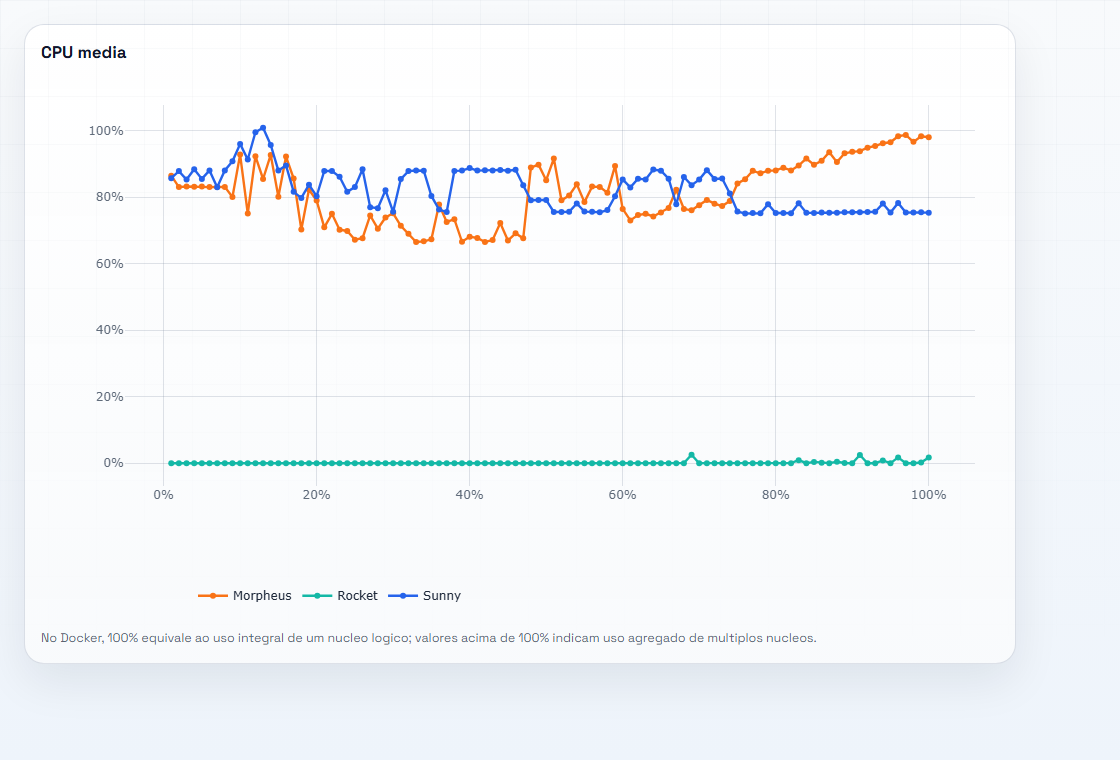
\includegraphics[width=0.9\linewidth,keepaspectratio]{figuras/benchmark/Figura_49_dashboard_cpu_i3_taxa_crossover.png}
\fonteautores
\notaacademica{100\% de CPU representa aproximadamente o uso integral de um núcleo lógico na telemetria do Docker; valores superiores indicam uso agregado de múltiplos núcleos.}
\end{figure}

\begin{figure}[H]
\centering
\caption{Uso médio de RAM na variação da taxa de crossover no cenário i3, conforme visualização filtrada no Dashboard IGRIS}
\label{fig:benchmark-ram-i3-crossover}
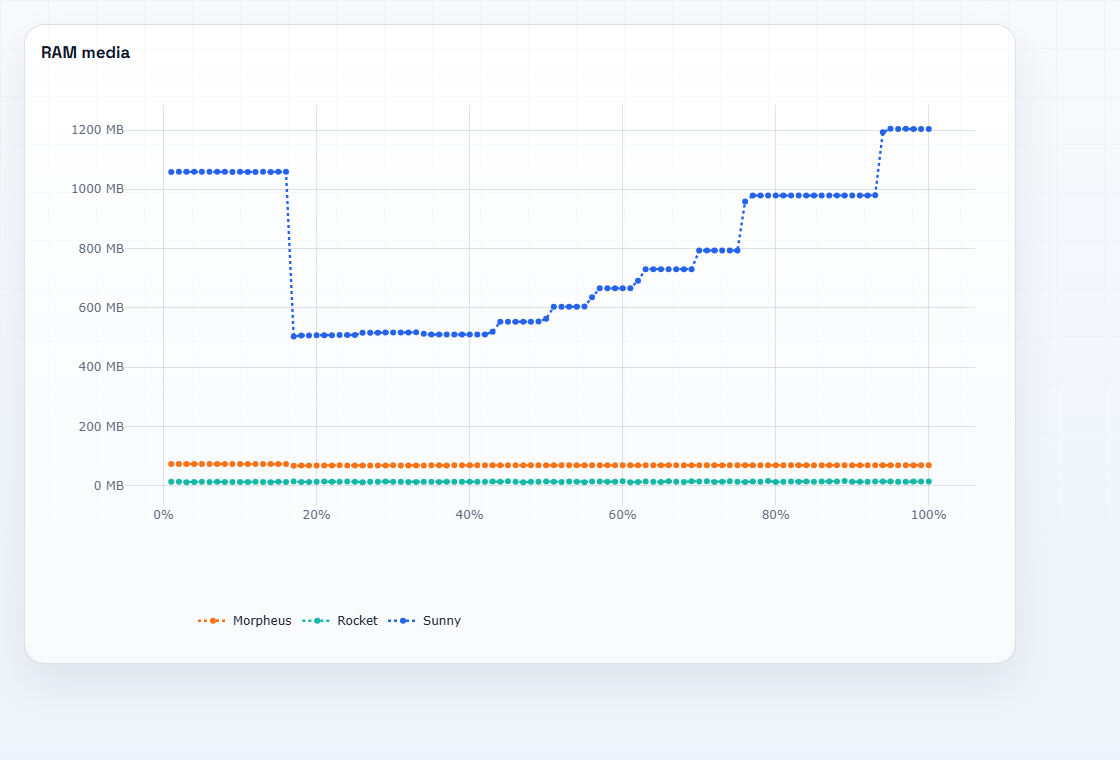
\includegraphics[width=0.9\linewidth,keepaspectratio]{figuras/benchmark/Figura_50_dashboard_ram_i3_taxa_crossover.png}
\fonteautores
\end{figure}

Essa diferença de memória pode estar relacionada ao conjunto formado por arquitetura do microsserviço, runtime utilizado, framework adotado, estrutura de dados e gerenciamento interno de memória. No caso do Sunny, a execução sobre o ecossistema Java pode contribuir para maior ocupação de memória. No caso do Rocket, a implementação em Go, a organização dos índices e o uso de estruturas mais compactas podem ter contribuído para o menor consumo. Entretanto, como os relatórios não apresentam profiling de heap, logs de Garbage Collector ou rastreamento detalhado de alocação, essa explicação deve ser tratada como hipótese, e não como conclusão definitiva.

No comportamento evolutivo, o Morpheus apresentou média de 191,38 gerações, o Rocket apresentou média de 191,52 gerações e o Sunny apresentou média de 945 gerações. Além disso, o Morpheus acionou parada antecipada em 8.979 execuções, o Rocket em 8.980 execuções e o Sunny não apresentou ocorrências de early stop. Esse dado indica que, na maior parte das execuções, Morpheus e Rocket encontraram um ponto de estabilização antes do limite máximo de gerações.

O erro médio foi igual para os três algoritmos, com valor de 3,00. Já o melhor score foi igual entre Morpheus e Rocket, com -29.574, e ligeiramente inferior no Sunny, com -29.640. Como valores menos negativos representam melhor avaliação relativa, Morpheus e Rocket tiveram pequena vantagem nessa métrica. No entanto, a diferença absoluta entre os scores é baixa em relação às penalidades utilizadas pela função \textit{fitness}, o que exige cautela na interpretação.

Diante dos resultados do cenário i3, o Rocket apresentou o melhor desempenho operacional, principalmente em tempo de resposta e consumo de memória. O Morpheus permaneceu superior ao Sunny nas métricas operacionais, enquanto o Sunny manteve taxa de sucesso total, mas exigiu mais memória e executou mais gerações sem apresentar redução no erro médio final.

\section{Cenário B -- Desempenho no Ambiente i5/full}
\label{sec:cenario-b-i5-full}

No cenário i5/full, cada algoritmo também foi submetido a 9.000 requisições. Nesse ambiente, os três algoritmos apresentaram taxa de sucesso de 100,00\%, o que indica que todos conseguiram concluir todas as execuções registradas no benchmark.

A latência média novamente favoreceu o Rocket. O algoritmo apresentou média de 640,26 ms, enquanto o Morpheus apresentou 5.044,99 ms e o Sunny apresentou 5.832,73 ms. Na comparação entre Morpheus e Sunny, a diferença representa uma latência média aproximadamente 15,61\% maior para o Sunny. Em comparação com o cenário i3, a vantagem relativa do Morpheus sobre o Sunny tornou-se ainda mais evidente, mas a presença do Rocket mostra uma terceira faixa de desempenho operacional, substancialmente inferior em tempo de resposta.

O p95 também manteve o mesmo padrão. O Rocket registrou 777,92 ms, enquanto o Morpheus registrou 6.058,92 ms e o Sunny registrou 7.083,80 ms. Na comparação entre Morpheus e Sunny, isso representa uma diferença de aproximadamente 16,92\% em favor do Morpheus. Portanto, no cenário i5/full, o Rocket apresentou melhor comportamento nas execuções mais lentas, e o Morpheus também manteve vantagem sobre o Sunny.

No consumo de memória, o Rocket utilizou em média 11,35 MB de RAM, com pico de 20,68 MB. O Morpheus utilizou em média 72,69 MB de RAM, com pico de 73,63 MB. O Sunny utilizou em média 778,60 MB de RAM, com pico de 1.098,75 MB. Embora o consumo médio do Sunny tenha sido menor no i5/full do que no i3, ele permaneceu muito superior ao consumo observado no Morpheus e no Rocket.

A diferença de gerações também permaneceu estável. O Rocket executou, em média, 191,44 gerações, o Morpheus executou 191,41 gerações e o Sunny executou 945 gerações. O Morpheus e o Rocket registraram 8.980 ocorrências de parada antecipada, enquanto o Sunny novamente não registrou early stop. Esse comportamento reforça que os algoritmos seguem dinâmicas evolutivas distintas, com Morpheus e Rocket interrompendo a execução antes do limite máximo na maior parte das requisições.

A parada antecipada no Morpheus e no Rocket indica que os algoritmos deixaram de executar antes do limite máximo de gerações na maior parte das requisições. Isso pode ocorrer quando não há melhoria significativa no \textit{fitness} durante uma determinada janela de gerações. Dessa forma, os algoritmos evitam continuar processando quando a população já se encontra estabilizada segundo o critério adotado.

O Sunny, por outro lado, executou próximo ao limite máximo de gerações. Isso não significa necessariamente pior qualidade evolutiva, mas indica maior custo computacional para atingir uma solução com erro médio equivalente ao dos demais algoritmos. Como os três encerraram com erro médio igual a 3,00, o maior número de gerações do Sunny não resultou, nos dados analisados, em eliminação adicional de inconsistências.

Quanto ao score, o Morpheus e o Rocket mantiveram o valor de -29.574, enquanto o Sunny manteve -29.640. A diferença novamente favorece Morpheus e Rocket, mas deve ser interpretada como vantagem pequena. O dado mais relevante do cenário i5/full é, portanto, a combinação entre menor latência, menor p95, menor consumo de memória e mesmo erro médio final observada no Rocket, seguida pelo desempenho operacional do Morpheus em relação ao Sunny.

Diante dos resultados, o cenário i5/full confirma o comportamento observado no cenário i3. O Rocket apresentou o melhor desempenho operacional, o Morpheus permaneceu mais eficiente que o Sunny, e o Sunny consumiu mais memória e executou mais gerações sem obter vantagem final no erro médio.

\section{Cenário C -- Análise por Parâmetro}
\label{sec:cenario-c-parametro}

Além da comparação geral entre os algoritmos, o benchmark também avaliou o comportamento das implementações diante da variação de parâmetros evolutivos. Os parâmetros analisados foram taxa de \textit{crossover}, tamanho da população, número de gerações, taxa de elitismo, pontuação base, penalidade de conflito, bônus de diversidade, tamanho do torneio e taxa de mutação.

Essa análise é importante porque algoritmos genéticos são sensíveis à configuração dos seus parâmetros. Alterações na taxa de \textit{crossover} podem modificar a capacidade de recombinação da população. Mudanças na taxa de mutação podem aumentar ou reduzir a diversidade genética. O tamanho da população influencia a quantidade de soluções candidatas avaliadas a cada geração. Já o número de gerações define por quanto tempo o algoritmo poderá evoluir suas soluções.

Nos dados analisados originalmente entre Morpheus e Sunny, o Morpheus apresentou menor tempo médio na maioria dos parâmetros avaliados. No cenário i3, o maior diferencial médio apareceu na taxa de \textit{crossover}, parâmetro em que o Sunny ficou 27,93\% acima do tempo médio do Morpheus. No cenário i5/full, a taxa de \textit{crossover} também apresentou o maior diferencial, com o Sunny 33,03\% acima do tempo médio do Morpheus.

Esse resultado indica que, nas variações relacionadas ao \textit{crossover}, o Morpheus apresentou melhor comportamento operacional que o Sunny. Como o \textit{crossover} é uma etapa executada repetidamente ao longo do processo evolutivo, diferenças de implementação nessa operação podem ter impacto relevante no tempo total de execução.

\begin{figure}[H]
\centering
\caption{Latência média na variação da taxa de crossover no Cenário i3, conforme visualização filtrada no Dashboard IGRIS}
\label{fig:benchmark-latencia-crossover-i3}
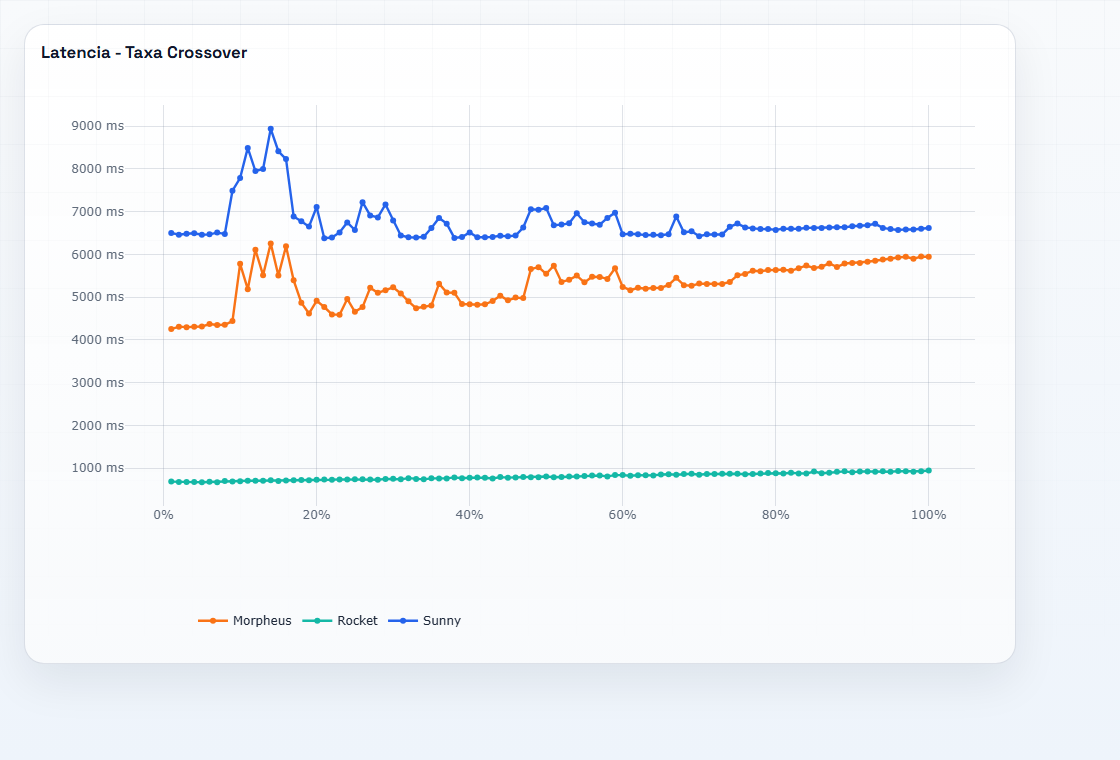
\includegraphics[width=0.9\linewidth,keepaspectratio]{figuras/benchmark/Figura_51_dashboard_latencia_i3_taxa_crossover.png}
\fonteautores
\end{figure}

\begin{figure}[H]
\centering
\caption{Latência média na variação da taxa de crossover no Cenário i5/full, conforme visualização filtrada no Dashboard IGRIS}
\label{fig:benchmark-latencia-crossover-i5}
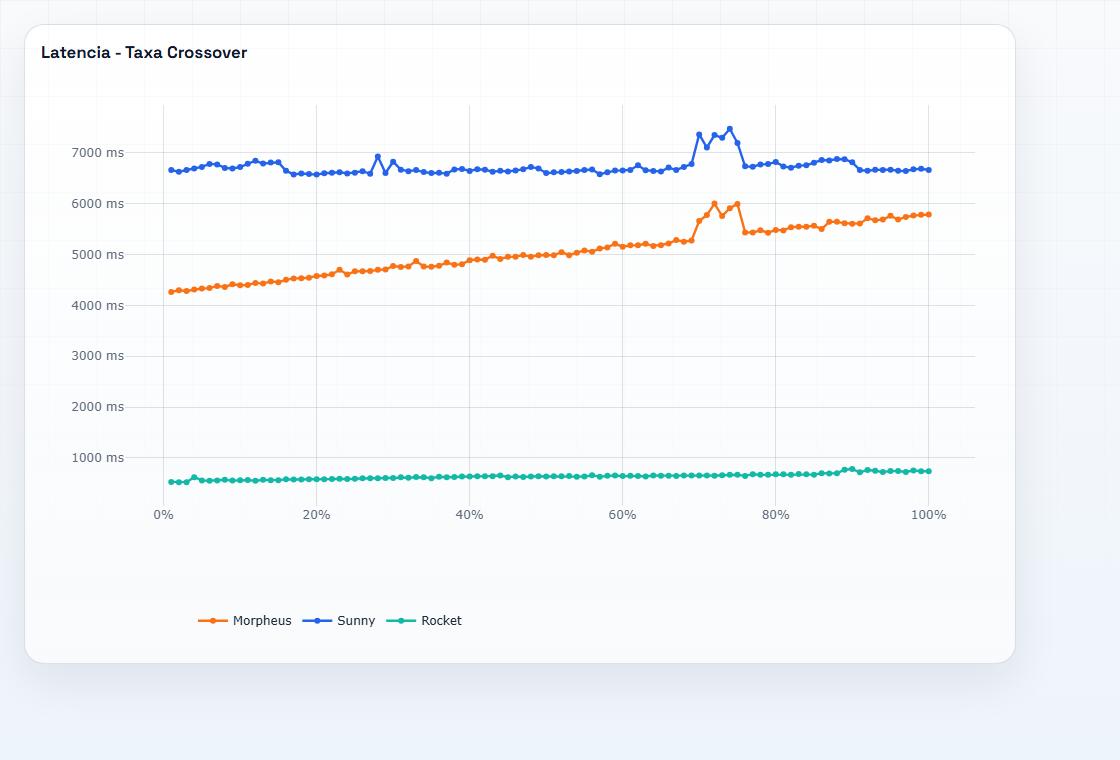
\includegraphics[width=0.9\linewidth,keepaspectratio]{figuras/benchmark/Figura_52_dashboard_latencia_i5_taxa_crossover.png}
\fonteautores
\end{figure}

Em parâmetros como tamanho da população, número de gerações, taxa de elitismo, pontuação base, penalidade de conflito, bônus de diversidade e tamanho do torneio, o Morpheus também apresentou médias de tempo inferiores às do Sunny. Esse comportamento reforça que sua vantagem não ocorreu apenas em um recorte específico, mas apareceu em diferentes dimensões do benchmark.

A principal exceção observada na comparação entre Morpheus e Sunny foi a taxa de mutação. Nesse parâmetro, o Sunny apresentou tempo médio menor nos dois cenários. No cenário i3, sua vantagem foi de aproximadamente 9,50\%. No cenário i5/full, a vantagem foi de aproximadamente 6,19\%. Esse resultado mostra que o Sunny pode apresentar desempenho competitivo em configurações específicas, mesmo não superando o Morpheus no agregado global.

\begin{figure}[H]
\centering
\caption{Latência média na variação da taxa de mutação no Cenário i3, conforme visualização filtrada no Dashboard IGRIS}
\label{fig:benchmark-latencia-mutacao-i3}
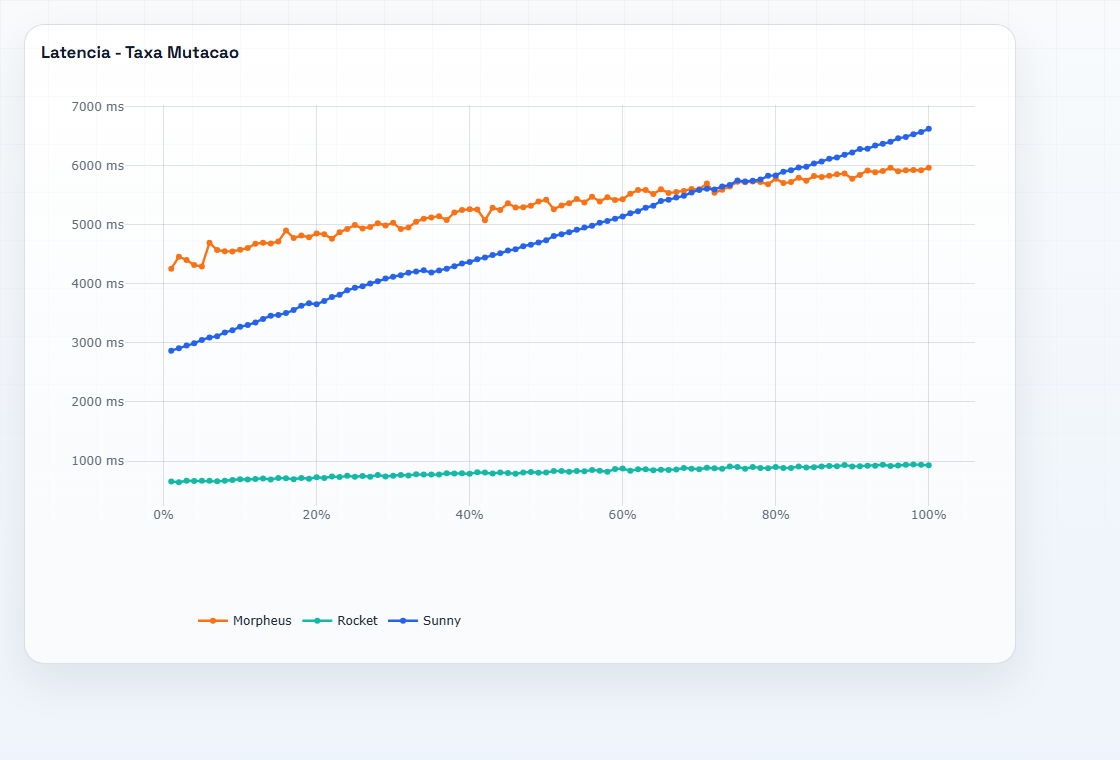
\includegraphics[width=0.9\linewidth,keepaspectratio]{figuras/benchmark/Figura_53_dashboard_latencia_i3_taxa_mutacao.png}
\fonteautores
\end{figure}

\begin{figure}[H]
\centering
\caption{Latência média na variação da taxa de mutação no Cenário i5/full, conforme visualização filtrada no Dashboard IGRIS}
\label{fig:benchmark-latencia-mutacao-i5}
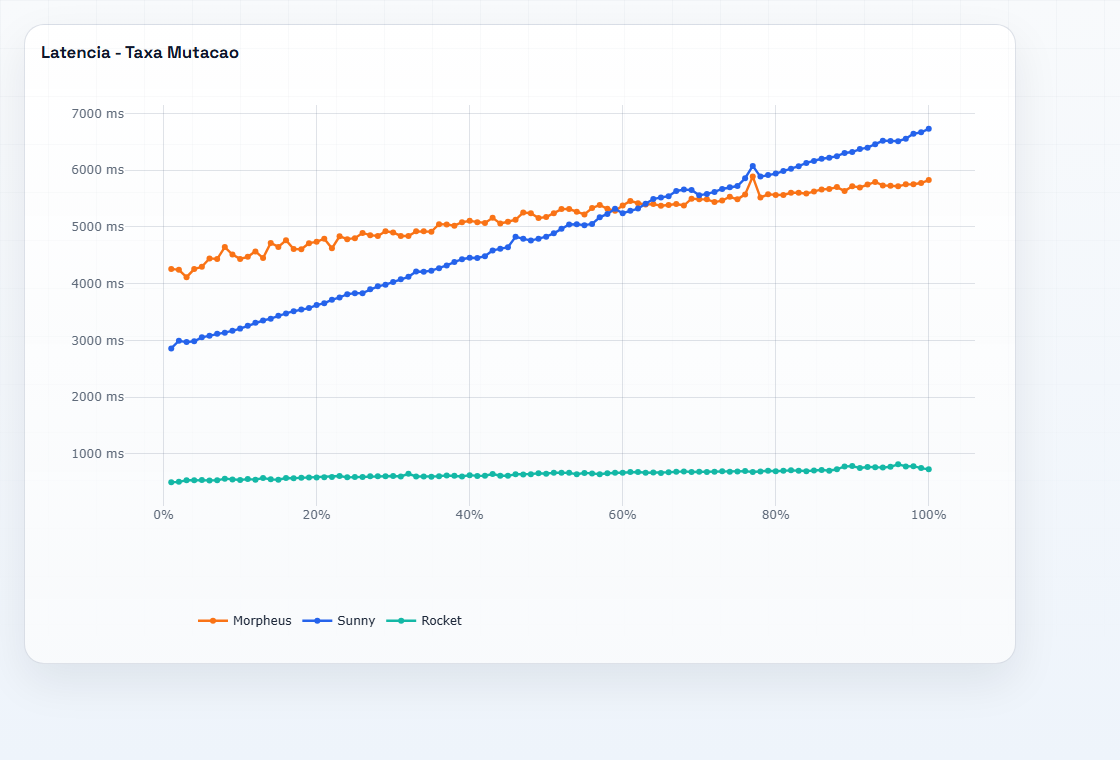
\includegraphics[width=0.9\linewidth,keepaspectratio]{figuras/benchmark/Figura_54_dashboard_latencia_i5_taxa_mutacao.png}
\fonteautores
\end{figure}

A incorporação do Rocket amplia essa leitura. No cenário i3, as maiores médias do Rocket ocorreram em taxa de elitismo, com 946,65 ms, tamanho do torneio, com 946,01 ms, penalidade de conflito, com 924,98 ms, bônus de diversidade, com 922,08 ms, e pontuação base, com 913,11 ms. No cenário i5/full, as maiores médias ocorreram em taxa de elitismo, com 738,94 ms, tamanho do torneio, com 734,23 ms, bônus de diversidade, com 732,38 ms, pontuação base, com 727,94 ms, e penalidade de conflito, com 727,61 ms.

Mesmo nos parâmetros mais custosos para o Rocket, suas médias permaneceram inferiores às médias observadas para Morpheus e Sunny nos mesmos cenários. No i3, por exemplo, os parâmetros menos custosos para Morpheus ficaram acima de 3.000 ms, enquanto o Rocket permaneceu abaixo de 1.000 ms em todos os agrupamentos paramétricos. No i5/full, o comportamento foi semelhante, com o Rocket abaixo de 740 ms nos agrupamentos de maior latência média e os demais algoritmos em patamares superiores.

Essa diferença pode indicar que o custo das operações evolutivas do Rocket foi reduzido pela combinação de estruturas indexadas, população e \textit{fitness} avaliados de forma concorrente e reparo local restrito a candidatos já filtrados. Entretanto, os dados não isolam o efeito de cada componente arquitetural. Portanto, não é possível afirmar se a vantagem decorre principalmente da linguagem, do modelo de concorrência, das estruturas de dados, da implementação do reparo ou da combinação desses fatores.

A análise por parâmetro deve ser interpretada com cautela, pois os resultados representam agrupamentos experimentais do benchmark progressivo. Portanto, não se trata necessariamente de um experimento isolado em que apenas uma variável foi alterada sob controle absoluto. Ainda assim, os dados permitem identificar em quais dimensões paramétricas as diferenças entre os algoritmos se tornaram mais evidentes.

De modo geral, o Rocket apresentou o menor tempo médio ao longo dos parâmetros avaliados, o Morpheus apresentou maior consistência operacional que o Sunny na maioria dos parâmetros, e o Sunny demonstrou vantagem pontual sobre o Morpheus na taxa de mutação. Dessa forma, a análise paramétrica confirma a tendência observada nos resultados gerais e mostra que a inclusão do Rocket revela um nível adicional de eficiência que não era observável na comparação apenas entre Morpheus e Sunny.

\section{Comparação do Comportamento Evolutivo}
\label{sec:comportamento-evolutivo}

A análise das gerações executadas mostra uma das principais diferenças entre os algoritmos. O Morpheus apresentou média próxima de 191 gerações nos dois cenários, o Rocket também apresentou média próxima de 191 gerações, enquanto o Sunny apresentou média de 945 gerações. Essa diferença indica que Morpheus e Rocket encerraram suas execuções de forma antecipada com muito mais frequência.

Nos dois cenários, o Morpheus registrou quase 9.000 ocorrências de parada antecipada. No cenário i3, foram 8.979 ocorrências. No cenário i5/full, foram 8.980. Considerando que cada cenário possui 9.000 requisições para o Morpheus, conclui-se que a parada antecipada foi predominante. O Rocket apresentou comportamento equivalente, com 8.980 ocorrências de parada antecipada tanto no i3 quanto no i5/full. O Sunny, por outro lado, não registrou ocorrências desse tipo nos relatórios analisados.

A parada antecipada pode representar uma vantagem operacional quando evita processamento desnecessário. Se o algoritmo passa várias gerações sem melhorar o \textit{fitness}, continuar executando até o limite máximo pode aumentar o tempo de resposta sem produzir ganho significativo na solução. Nesse sentido, o comportamento do Morpheus e do Rocket contribuiu para reduzir o número médio de gerações executadas.

Entretanto, essa métrica não deve ser interpretada isoladamente como prova de superioridade evolutiva. Um algoritmo pode parar cedo porque encontrou uma boa solução rapidamente, mas também pode parar porque atingiu um platô de melhoria. Por isso, a análise precisa considerar as demais métricas, como score e erro médio.

O Sunny, por sua vez, executou próximo ao limite máximo de gerações na maior parte das execuções. Esse comportamento está relacionado ao fato de sua dinâmica evolutiva depender da continuidade dos ciclos de seleção, \textit{crossover}, mutação, avaliação e elitismo até o limite configurado. Como não houve registro de parada antecipada nos relatórios, o algoritmo manteve uma execução mais prolongada.

O erro médio final foi igual para os três algoritmos, permanecendo em 3,00 nos dois cenários. Isso indica que, apesar de executar mais gerações, o Sunny não conseguiu reduzir o erro médio abaixo do resultado obtido pelo Morpheus e pelo Rocket. Por outro lado, Morpheus e Rocket também não eliminaram completamente os erros restantes, mesmo com melhor desempenho operacional.

A métrica de melhor geração média também exige cautela. No Morpheus, o melhor indivíduo aparece, em média, nas primeiras gerações, com média de 1,25 no i3 e 1,27 no i5/full. No Rocket, esse comportamento é semelhante, com média de 1,39 no i3 e 1,31 no i5/full. Esse padrão pode indicar que soluções de alto \textit{fitness} já foram produzidas na população inicial, que os mecanismos de reparo tiveram forte impacto no início da execução ou que a população rapidamente atingiu uma região de estabilização. Sem detalhamento adicional dos registros, não é possível afirmar qual desses fatores foi determinante.

No caso do Sunny, a média de melhor geração foi mais alta, com 20,16 no i3 e 20,92 no i5/full, além de maior permanência no ciclo evolutivo. No entanto, como o erro médio e o score final não superaram os de Morpheus e Rocket, o custo adicional de execução não se traduziu em vantagem final nas métricas disponíveis.

A presença do Rocket torna mais clara a distinção entre número de gerações e custo de execução. Morpheus e Rocket executaram quantidades médias de gerações praticamente equivalentes, mas o Rocket apresentou latência e consumo de memória muito inferiores. Isso sugere que a diferença operacional entre eles não decorre apenas do critério de parada, mas também do custo por geração, da organização interna dos dados e da forma como população, \textit{fitness} e reparo são executados.

\section{Score e Erro Médio}
\label{sec:score-erro-medio}

O score final é uma métrica importante porque resume a avaliação da solução segundo a função \textit{fitness}. Como a função aplica penalidades, scores menos negativos indicam soluções relativamente melhores. Nos dois cenários avaliados, o Morpheus e o Rocket apresentaram melhor score, com -29.574, enquanto o Sunny apresentou -29.640.

A diferença entre Morpheus e Sunny foi de 66 pontos, e a diferença entre Rocket e Sunny também foi de 66 pontos. Embora essa diferença favoreça Morpheus e Rocket, ela é pequena quando comparada à escala das penalidades utilizadas na função \textit{fitness}. Penalidades de conflito podem assumir valores muito superiores a essa diferença absoluta, o que significa que o score, isoladamente, não sustenta uma conclusão forte sobre superioridade qualitativa.

O erro médio, por sua vez, foi igual para os três algoritmos. Todos terminaram com erro médio 3,00 nos cenários i3 e i5/full. Esse dado é relevante porque mostra que nenhum dos algoritmos conseguiu produzir, em média, soluções completamente livres de inconsistências.

A interpretação do erro médio é limitada pela ausência de decomposição homogênea dos tipos de erro nos relatórios consolidados. Três inconsistências podem representar problemas de baixa gravidade, corrigíveis manualmente, ou conflitos estruturais capazes de inviabilizar o uso direto da grade. Sem essa informação, não é possível afirmar se as soluções finais são diretamente utilizáveis sem revisão.

Dessa forma, a comparação entre os algoritmos é mais robusta nas métricas operacionais do que nas métricas qualitativas. O Rocket foi mais rápido, consumiu menos memória e teve score equivalente ao do Morpheus. O Morpheus, por sua vez, foi mais rápido e consumiu menos memória que o Sunny, além de apresentar score ligeiramente melhor. Entretanto, os três mantiveram o mesmo erro médio final. Portanto, a vantagem do Rocket e do Morpheus em relação ao Sunny deve ser descrita principalmente como operacional, e não como evidência suficiente de superioridade qualitativa completa das grades geradas.

\section{Limitações dos Testes}
\label{sec:limitacoes-testes}

Apesar de o benchmark permitir uma comparação objetiva entre Morpheus, Sunny e Rocket, algumas limitações devem ser consideradas. A primeira delas está relacionada ao ambiente de execução. Os relatórios não detalham completamente as configurações de hardware e software utilizadas em cada cenário. Informações como processador exato, quantidade de núcleos, memória disponível, sistema operacional, versões de runtime, uso de container e limites de CPU ou RAM não estão completamente especificadas.

Essa ausência limita a reprodutibilidade exata dos testes. Em benchmarks computacionais, pequenas diferenças no ambiente podem afetar métricas como tempo de execução, consumo de memória e uso de CPU. Por isso, os resultados devem ser entendidos como válidos para o protocolo analisado, e não como medidas absolutas independentes do ambiente.

Outra limitação está relacionada ao controle da aleatoriedade. Algoritmos genéticos dependem de processos estocásticos, como seleção, \textit{crossover}, mutação e geração da população inicial. Os relatórios não informam as sementes aleatórias utilizadas nas execuções. Dessa forma, embora as repetições reduzam parte da variabilidade, a reprodução exata dos resultados fica limitada.

Também não há detalhamento completo e homogêneo sobre a composição do erro médio. Como essa métrica não é decomposta por tipo de violação de forma suficiente para sustentar comparação qualitativa aprofundada, não é possível identificar, a partir da síntese apresentada, se os erros restantes correspondem a choques de professor, choques de turma, horários inválidos, demandas não alocadas ou outro tipo de inconsistência. Essa limitação impede uma avaliação mais profunda da qualidade acadêmica das grades geradas.

Além disso, as métricas de CPU devem ser interpretadas com cautela. A coleta foi baseada na telemetria do Docker para os containers monitorados, em que 100\% de CPU representa aproximadamente o uso integral de um núcleo lógico, e não necessariamente a ocupação de todo o host físico. Ainda assim, os relatórios não detalham completamente possíveis interferências externas, concorrência, aquecimento, janela exata de amostragem ou descarte de outliers. Essa cautela é especialmente relevante no caso do Rocket, pois a média de CPU registrada foi baixa, enquanto os picos foram elevados, o que pode refletir características da coleta por amostragem, execução concorrente concentrada em intervalos curtos ou particularidades do ambiente de medição.

Outra limitação decorre do fato de os relatórios do Rocket terem sido gerados separadamente dos relatórios de Morpheus e Sunny, embora com o mesmo perfil de \textit{payload} e os mesmos cenários declarados. Essa separação não invalida a comparação descritiva, mas recomenda cautela adicional, pois diferenças de momento de execução, estado do host, versão de container ou condições de carga podem afetar métricas operacionais.

Por fim, a análise apresentada é predominantemente descritiva. Não foram aplicados testes estatísticos inferenciais, intervalos de confiança ou análise formal de significância entre os três algoritmos. Assim, os resultados devem ser interpretados como evidências experimentais do benchmark executado, e não como comprovação estatística universal de superioridade de um algoritmo sobre o outro.

\section{Síntese dos Resultados}
\label{sec:sintese-resultados}

Os resultados obtidos no benchmark indicam que o Rocket apresentou o melhor desempenho operacional entre os três algoritmos nos dois cenários avaliados. Essa vantagem aparece principalmente na latência média, no percentil 95 da latência e no consumo de memória RAM. O Rocket também apresentou número médio de gerações semelhante ao Morpheus, em razão da ocorrência frequente de parada antecipada.

No cenário i3, o Rocket foi mais rápido tanto na média quanto no p95, além de consumir menos memória que Morpheus e Sunny. O Morpheus foi mais rápido que o Sunny e consumiu muito menos memória, preservando a conclusão da comparação original entre os dois algoritmos. No cenário i5/full, o mesmo comportamento foi mantido, com vantagem operacional do Rocket e vantagem do Morpheus sobre o Sunny na latência média, no p95 e no consumo de memória.

O Sunny apresentou taxa de sucesso total nos dois cenários e teve desempenho pontualmente melhor que o Morpheus na análise do parâmetro taxa de mutação. Também deve ser considerado que sua implementação não se limita à penalização pura, pois utiliza organização interna dos dados, inicialização guiada por restrições e reparo parcial. Ainda assim, no resultado agregado do benchmark, o Sunny consumiu mais memória, executou mais gerações e não obteve redução no erro médio final em relação ao Morpheus e ao Rocket.

A comparação de score favoreceu Morpheus e Rocket, mas com diferença pequena em relação ao Sunny. O erro médio permaneceu igual para os três algoritmos, com valor de 3,00. Assim, não é possível afirmar que Rocket ou Morpheus produziram grades completamente válidas ou qualitativamente superiores em todos os aspectos. O que os dados sustentam com maior clareza é que Rocket e Morpheus produziram resultados equivalentes no erro médio com menor custo operacional que o Sunny, sendo o Rocket o algoritmo com menor custo operacional entre os três.

A inclusão do Rocket revela uma dimensão que a comparação anterior entre Morpheus e Sunny não permitia observar. Como Morpheus e Rocket apresentaram número médio de gerações e frequência de parada antecipada muito semelhantes, mas tempos e consumos de memória bastante diferentes, os resultados sugerem que a eficiência não depende apenas de encerrar o ciclo evolutivo mais cedo. Ela também pode estar associada ao custo por geração, ao modelo de organização dos dados, à avaliação paralela da população, ao reparo local e ao gerenciamento de memória da implementação.

Dessa forma, considerando o \textit{payload}, os parâmetros e o ambiente avaliados, o Rocket mostrou-se mais adequado para o contexto analisado sob a perspectiva operacional. O Morpheus manteve-se como alternativa mais eficiente que o Sunny, enquanto o Sunny demonstrou estabilidade de execução, mas com maior custo de memória e maior número de gerações. Essa conclusão, contudo, está restrita ao protocolo de benchmark executado e não deve ser generalizada como superioridade universal de linguagem, arquitetura ou abordagem evolutiva.


\chapter{Considerações Finais e Conclusões}
\label{cap:consideracoes}

Este trabalho teve como objetivo propor uma solução computacional para o problema de alocação semestral de grades horárias em Instituições de Ensino Superior, por meio do desenvolvimento do IGRIS, um sistema modular de suporte à decisão baseado em Algoritmos Genéticos. A proposta partiu da necessidade de automatizar um processo tradicionalmente conduzido de forma manual, caracterizado por elevada complexidade combinatória e pela necessidade de considerar simultaneamente disciplinas, turmas, docentes, disponibilidades e restrições acadêmicas.

A solução desenvolvida demonstrou que o uso de Algoritmos Genéticos é uma alternativa tecnicamente viável para apoiar a geração automatizada de grades horárias acadêmicas. Por meio da representação das alocações como soluções candidatas, foi possível aplicar operadores evolutivos, como seleção, \textit{crossover}, mutação e elitismo, com o objetivo de explorar diferentes combinações de horários e buscar arranjos mais adequados às restrições do problema. Dessa forma, o IGRIS contribui para reduzir o esforço manual envolvido na montagem das grades e para apoiar os coordenadores acadêmicos no processo de tomada de decisão.

A arquitetura modular adotada também se mostrou adequada aos objetivos do trabalho, pois permitiu separar as responsabilidades entre interface, persistência, serviços de apoio e módulos de otimização. Essa organização favorece a manutenção do sistema, a evolução independente dos componentes e a inclusão de diferentes implementações algorítmicas dentro de uma mesma estrutura de integração. Com isso, o IGRIS não se limita a uma única estratégia de geração de grades, mas oferece uma base para avaliar e comparar diferentes abordagens aplicadas ao \textit{University Course Timetabling Problem}.

No desenvolvimento do sistema, a modelagem das entidades acadêmicas e dos fluxos de operação foi essencial para aproximar o problema real de sua representação computacional. A definição de turmas, disciplinas, docentes, disponibilidades, matrizes curriculares e vínculos permitiu estruturar os dados necessários ao funcionamento dos algoritmos. Essa etapa foi fundamental, pois a qualidade da solução gerada depende diretamente da forma como as informações acadêmicas são organizadas e disponibilizadas para processamento.

As implementações dos algoritmos Morpheus, Sunny e Rocket permitiram avaliar diferentes decisões de projeto aplicadas ao mesmo domínio. Embora os três utilizem princípios fundamentais dos Algoritmos Genéticos, eles diferem em aspectos como organização interna dos dados, tratamento de conflitos, dinâmica de execução, uso de parada antecipada, avaliação da população e consumo de recursos computacionais. Nos cenários analisados, o Rocket apresentou o melhor desempenho operacional, com menores valores de latência média, percentil 95 e consumo de memória RAM. O Morpheus manteve desempenho superior ao Sunny nas métricas operacionais agregadas, enquanto o Sunny apresentou taxa de sucesso elevada e comportamento competitivo em determinados recortes de parametrização, ainda que com maior uso de memória e maior número médio de gerações no conjunto geral dos testes.

Os resultados obtidos indicam que a comparação entre as implementações deve ser compreendida principalmente sob a perspectiva de eficiência computacional. Embora Rocket e Morpheus tenham apresentado melhor desempenho em tempo de resposta, consumo de recursos e score final em relação ao Sunny, os três algoritmos mantiveram erro médio final equivalente nos cenários avaliados. Assim, os dados não permitem afirmar que uma das implementações produza grades qualitativamente superiores em todos os aspectos, mas sustentam que o Rocket alcançou resultados equivalentes com menor custo operacional no protocolo experimental adotado, seguido pelo Morpheus em relação ao Sunny.

Também foi possível observar que a automação proposta não elimina a necessidade de validação humana. O IGRIS atua como uma ferramenta de apoio à decisão, oferecendo soluções candidatas, reduzindo o esforço operacional e organizando o processo de geração de grades. Entretanto, a análise final ainda cabe aos responsáveis acadêmicos, especialmente porque algumas restrições institucionais podem não estar completamente formalizadas no sistema ou depender de critérios administrativos específicos.

A interface web desenvolvida contribui para tornar a solução utilizável no contexto institucional, permitindo o cadastro de dados, a configuração dos parâmetros e a visualização dos resultados de forma organizada. Esse aspecto reforça o caráter aplicado do trabalho, pois a efetividade de uma solução computacional para gestão acadêmica não depende apenas do algoritmo de otimização, mas também da clareza da interação com o usuário, da consistência dos dados e da integração com o fluxo de trabalho dos coordenadores.

Apesar dos resultados alcançados, algumas limitações devem ser consideradas. Os testes realizados não contemplam todos os possíveis cenários acadêmicos, e os relatórios de benchmark não detalham integralmente aspectos como ambiente de execução, controle de aleatoriedade, decomposição dos erros finais e aplicação de critérios estatísticos inferenciais. Além disso, os relatórios do Rocket foram gerados separadamente dos relatórios de Morpheus e Sunny, ainda que com o mesmo perfil de \textit{payload} e os mesmos cenários declarados, o que recomenda cautela adicional na interpretação comparativa. Essas limitações indicam a necessidade de avaliações complementares com maior diversidade de dados, maior controle experimental e registro mais detalhado das condições de execução.

Como trabalhos futuros, recomenda-se ampliar os experimentos com bases acadêmicas de diferentes tamanhos e níveis de complexidade, além de decompor o erro médio por tipo de inconsistência, como conflito de professor, conflito de turma, demanda não alocada e incompatibilidade de disponibilidade. Também se recomenda incorporar mecanismos de observabilidade, como logs estruturados, métricas detalhadas de execução, profiling de memória, rastreamento de alocação, logs de Garbage Collector quando aplicável e registro das sementes aleatórias utilizadas, a fim de aumentar a rastreabilidade e a reprodutibilidade dos resultados.

Outra possibilidade de continuidade consiste na inclusão de novos módulos de otimização, baseados em técnicas como Simulated Annealing, Busca Tabu, Otimização por Enxame de Partículas ou abordagens híbridas. A arquitetura modular do IGRIS favorece essa expansão, permitindo que diferentes estratégias sejam integradas, executadas e comparadas conforme o perfil do problema acadêmico analisado.

Conclui-se, portanto, que o objetivo do trabalho foi alcançado, uma vez que foi proposta e desenvolvida uma solução computacional modular para apoiar a geração automatizada de grades horárias em Instituições de Ensino Superior. O IGRIS demonstrou capacidade de representar o problema de alocação acadêmica, aplicar Algoritmos Genéticos à geração de soluções candidatas, reduzir o esforço manual dos coordenadores e permitir a avaliação comparativa entre diferentes implementações evolutivas. Embora existam limitações experimentais e oportunidades de aprimoramento, os resultados obtidos indicam que a solução proposta constitui uma base consistente para a evolução de ferramentas computacionais de apoio à gestão acadêmica.




% --- Fase Pós-Textual ---
% Elementos complementares ao texto, sem numeração de capítulo, mas indexados no sumário
\postextual

\bibliography{postextuais/referencias}

\chapter*{APÊNDICE A -- RECURSOS DIGITAIS COMPLEMENTARES DOS BENCHMARKS}
\addcontentsline{toc}{chapter}{APÊNDICE A -- RECURSOS DIGITAIS COMPLEMENTARES DOS BENCHMARKS}

\setcounter{figure}{0}
\renewcommand{\thefigure}{A.\arabic{figure}}
\setcounter{table}{0}
\renewcommand{\thetable}{A.\arabic{table}}
\renewcommand{\tablename}{Quadro}

Este apêndice apresenta os recursos digitais complementares utilizados na análise dos benchmarks do sistema IGRIS. Os materiais estão organizados em quatro blocos, correspondentes aos conjuntos de imagens utilizados na avaliação comparativa dos algoritmos e ao painel digital com os resultados completos dos benchmarks. Cada bloco pode ser acessado por meio de código QR e endereço eletrônico público.

As imagens disponibilizadas correspondem às versões digitais ampliadas das figuras apresentadas no corpo do trabalho, com a finalidade de facilitar a consulta visual dos gráficos e preservar a legibilidade dos dados analisados.

\begin{figure}[H]
\centering
\caption{Código QR para acesso às imagens do Bloco 1 (figuras)}
\label{fig:apendice-qr-bloco-1}

\includegraphics[width=0.38\textwidth,keepaspectratio]{figuras/apendice/qr_code_pasta_1.png}
\fonteautores
\par{\footnotesize\raggedright Disponível em: \nolinkurl{https://dash-image.netlify.app/?category=bloco1}.\par}
{\footnotesize\raggedright Acesso em: 19 jun. 2026.\par}
\end{figure}

\begin{figure}[H]
\centering
\caption{Código QR para acesso às imagens do Bloco 2 (benchmark)}
\label{fig:apendice-qr-bloco-2}

\includegraphics[width=0.38\textwidth,keepaspectratio]{figuras/apendice/qr_code_pasta_2.png}
\fonteautores
\par{\footnotesize\raggedright Disponível em: \nolinkurl{https://dash-image.netlify.app/?category=bloco2}.\par}
{\footnotesize\raggedright Acesso em: 19 jun. 2026.\par}
\end{figure}

\begin{figure}[H]
\centering
\caption{Código QR para acesso às imagens do Bloco 3 (protótipo)}
\label{fig:apendice-qr-bloco-3}

\includegraphics[width=0.38\textwidth,keepaspectratio]{figuras/apendice/qr_code_pasta_3.png}
\fonteautores
\par{\footnotesize\raggedright Disponível em: \nolinkurl{https://dash-image.netlify.app/?category=bloco3}.\par}
{\footnotesize\raggedright Acesso em: 19 jun. 2026.\par}
\end{figure}

\begin{figure}[H]
\centering
\caption{Código QR para acesso ao dashboard completo dos benchmarks}
\label{fig:apendice-qr-benchmark-completo}

\includegraphics[width=0.38\textwidth,keepaspectratio]{figuras/apendice/qr_code_benchmark_completo.png}
\fonteautores
\par{\footnotesize\raggedright Disponível em: \nolinkurl{https://igris-dashboard.netlify.app/}.\par}
{\footnotesize\raggedright Acesso em: 14 jun. 2026.\par}
\end{figure}

\begin{longtable}{|L{2.2cm}|L{5.0cm}|L{2.5cm}|L{4.2cm}|}
\caption{Organização dos recursos digitais complementares}
\label{quad:organizacao-recursos-digitais}\\
\hline
\textbf{Bloco} & \textbf{Conteúdo disponibilizado} & \textbf{Pasta vinculada} & \textbf{Finalidade} \\
\hline
\endfirsthead
\hline
\textbf{Bloco} & \textbf{Conteúdo disponibilizado} & \textbf{Pasta vinculada} & \textbf{Finalidade} \\
\hline
\endhead
Bloco 1 & Imagens referentes às figuras do trabalho & Pasta 1 & Consulta ampliada das visualizações \\
\hline
Bloco 2 & Imagens referentes aos benchmarks & Pasta 2 & Consulta ampliada dos gráficos de desempenho \\
\hline
Bloco 3 & Imagens referentes ao protótipo & Pasta 3 & Consulta ampliada das telas e registros visuais \\
\hline
Bloco 4 & Dashboard completo dos benchmarks & Site público & Consulta interativa dos resultados experimentais \\
\hline
\end{longtable}

\fonteautores


\end{document}
